%% FIT CTU thesis template
%% https://gitlab.fit.cvut.cz/theses-templates/FITthesis-LaTeX

\documentclass[czech,bachelor,unicode]{ctufit-thesis}

%%%%%%%%%%%%%%%%%%%%%%%%%%%%%%%%%%
% BASIC INFORMATION
%%%%%%%%%%%%%%%%%%%%%%%%%%%%%%%%%%
\ctufittitle{Zpěvník pro náboženská shromáždění – mobilní aplikace}
\ctufitauthorfull{Ondřej Wrzecionko}
\ctufitauthorsurnames{Wrzecionko}
\ctufitauthorgivennames{Ondřej}
\ctufitsupervisor{Ing. Jan Matoušek}
\ctufitdepartment{Katedra softwarového inženýrství}
\ctufityear{2022}
\ctufitdeclarationplace{Praze}
\ctufitdeclarationdate{10. května 2022}

% Abstract and keywords
\ctufitabstractCZE{Práce se zabývá analýzou, návrhem, implementací, testováním a nasazením iOS a macOS aplikace zpěvníku pro náboženská shromáždění a podpůrného serveru poskytujícího REST API pro tuto mobilní aplikaci. Mobilní aplikace je implementována v programovacím jazyce Swift, podpůrný server v programovacím jazyce Kotlin s použitím technologie Spring Web. Aplikace umožňuje zobrazení a správu písní ve zpěvnících a přiřazení zpěvníků ke kapelám. V těchto kapelách je možná správa členů a jejich oprávnění (vedoucí spravuje členy a zpěvníky, hudebník spravuje písně, zpěváku jsou zobrazeny pouze písně a zpěvníky). Písním lze nastavit jejich text, akordy, velikost textu, tempo, výchozí transpozici a soukromé poznámky.

Aplikace je nasazena do obchodu pro iOS a macOS aplikace App Store, ze kterého ji za první měsíc nainstalovala a začala používat čtyři náboženská shromáždění, která do ní dosud nahrála přes 1000 písní v 10 zpěvnících.}
\ctufitabstractENG{Thesis deals with analysis, proposal, implementation, testing and deployment of iOS and macOS application of song book for religious gatherings and supporting server providing REST API for this mobile application. Application is implemented in programming language Swift, supporting server is implemented in programming language Kotlin with use of technology Spring Web. Application allows users to display and manage songs in song books and assign song books to bands. Within these bands, leader manages members and song books, musician manages songs and singers are shown only songs and song books. Users can set song lyrics, chords, lyrics font size, bpm, default transposition and private notes.

Application is deployed to iOS and macOS application store App Store. During first month, four religious gatherings started using the application and by now, over 1 000 songs in 10 song books have been added to the application.}

\ctufitkeywordsCZE{zpěvník, mobilní aplikace, REST API, náboženské shromáždění, iOS, macOS, Swift, Spring Web, Kotlin}
\ctufitkeywordsENG{songbook, mobile application, REST API, religious gathering, iOS, macOS, Swift, Spring Web, Kotlin}
%%%%%%%%%%%%%%%%%%%%%%%%%%%%%%%%%%
% END BASIC INFORMATION
%%%%%%%%%%%%%%%%%%%%%%%%%%%%%%%%%%

%%%%%%%%%%%%%%%%%%%%%%%%%%%%%%%%%%
% CUSTOMIZATION of template
%%%%%%%%%%%%%%%%%%%%%%%%%%%%%%%%%%

\RequirePackage{iftex}[2020/03/06]
\iftutex % XeLaTeX and LuaLaTeX
    \RequirePackage{ellipsis}[2020/05/22]
\else
    \RequirePackage[utf8]{inputenc}[2018/08/11]
    \RequirePackage{lmodern}[2009/10/30]
\fi

% hyperlinks
\RequirePackage[pdfpagelayout=TwoPageRight,colorlinks=false,allcolors=decoration,pdfborder={0 0 0.1}]{hyperref}[2020-05-15]

% TODO: ODKOMENTOVAT PRED TISKEM
% \RequirePackage[pdfpagelayout=TwoPageRight,hidelinks]{hyperref}[2020-05-15]

\RequirePackage{pdfpages}[2020/01/28]
\setcounter{secnumdepth}{4} % numbering sections; 4: subsubsection

%%%%%%%%%%%%%%%%%%%%%%%%%%%%%%%%%%
% CUSTOMIZATION of template END
%%%%%%%%%%%%%%%%%%%%%%%%%%%%%%%%%%

%%%%%%%%%%%%%%%%%%%%%%
% CONTENTS SETTINGS
%%%%%%%%%%%%%%%%%%%%%%
\usepackage{dirtree}
\usepackage{lipsum}
\usepackage{csquotes}
\usepackage[style=iso-numeric]{biblatex}
\addbibresource{text/bib-database.bib}
\usepackage{minted} % typesetting of sources
\usepackage{musicography}
\usemintedstyle{vs}
%%%%%%%%%%%%%%%%%%%%%%
% CONTENTS SETTINGS END
%%%%%%%%%%%%%%%%%%%%%%

% do not remove these two commands
\begin{document} 
\frontmatter\frontmatterinit

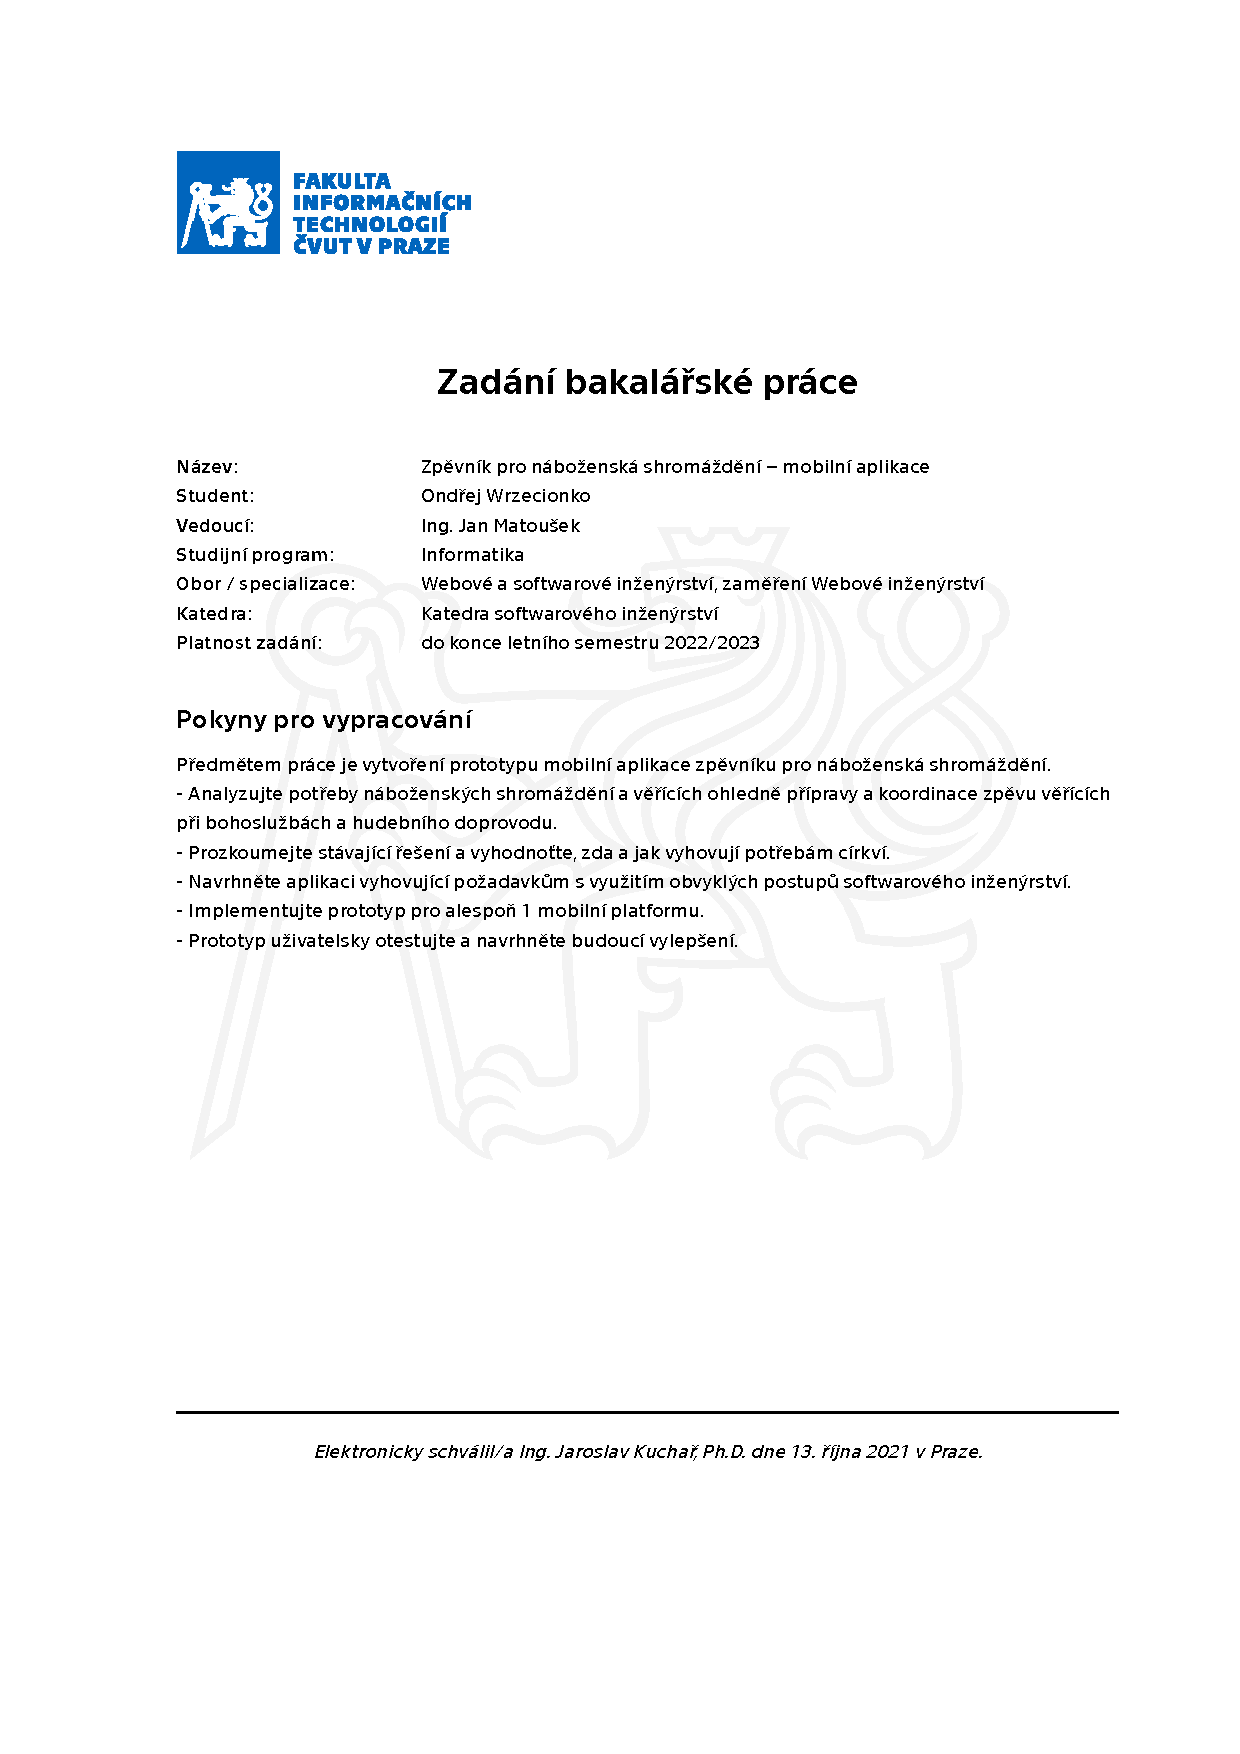
\includepdf{assignment-include.pdf}

% do not remove these commands
\thispagestyle{empty}\cleardoublepage\maketitle
\imprintpage
\tableofcontents

%%%%%%%%%%%%%%%%%%%%%%
% list of other contents: figures, tables, code listings, algorithms, etc.
% add/remove commands accordingly
%%%%%%%%%%%%%%%%%%%%%%
\listoffigures % list of figures
\begingroup
\let\clearpage\relax
\listoftables % list of tables
\listoflistings % list of source code listings generated by the minted package
\endgroup
%%%%%%%%%%%%%%%%%%%%%%
% list of other contents END
%%%%%%%%%%%%%%%%%%%%%%

%%%%%%%%%%%%%%%%%%%
% ACKNOWLEDGMENT
%%%%%%%%%%%%%%%%%%%
\begin{acknowledgmentpage}
	Chtěl bych poděkovat především svému vedoucímu, Ing. Janu Matouškovi, za jeho podporu a pomoc při tvorbě této bakalářské práce. Nadále bych chtěl poděkovat náboženským shromážděním v Českém Těšíně a Pyšelích za jejich spolupráci při tvorbě aplikace a v neposlední řadě rodině za její podporu při celém bakalářském studiu.
\end{acknowledgmentpage} 
%%%%%%%%%%%%%%%%%%%
% ACKNOWLEDGMENT END
%%%%%%%%%%%%%%%%%%%

%%%%%%%%%%%%%%%%%%%
% DECLARATION
%%%%%%%%%%%%%%%%%%%
\begin{declarationpage}
Prohlašuji, že jsem předloženou práci vypracoval samostatně a že jsem uvedl veškeré použité informační zdroje v souladu s Metodickým pokynem o dodržování etických principů při přípravě vysokoškolských závěrečných prací.
Beru na vědomí, že se na moji práci vztahují práva a povinnosti vyplývající ze zákona č.121/2000 Sb., autorského zákona, ve znění pozdějších předpisů, zejména skutečnost, že České vysoké učení technické v Praze má právo na uzavření licenční smlouvy o užití této práce jako školního díla podle § 60 odst. 1 citovaného zákona.
\end{declarationpage}
%%%%%%%%%%%%%%%%%%%
% DECLARATION END
%%%%%%%%%%%%%%%%%%%

% do not remove this command
\printabstractpage

%%%%%%%%%%%%%%%%%%%
% ABBREVIATIONS
%%%%%%%%%%%%%%%%%%%
\chapter{Seznam zkratek}
	
\begin{tabular}{rl}
AC & Apoštolská církev\\
API & Application Programming Interface\\
CRUD & Create Read Update Delete\\
DTO & Data Transfer Object\\
GraphQL & Graph Query Language\\
HATEOAS & Hypertext As The Engine of Application State\\
HTTP & HyperText Transfer Protocol\\
HTTPS & Hypertext Transfer Protocol Secure\\
JPQL & Jakarta Persistence Query Language\\
JSON & JavaScript Object Notation\\
KřSb & Křesťanské sbory\\
MVC & Model View Controller\\
MVVM & Model View ViewModel\\
PNŽ & Písně nového života\\
REST & Representational State Transfer\\
SOAP & Simple Object Access Protocol\\
SQL & Sequenced Query Language\\
UI & User Interface\\
WSDL & Web Service Definition Language\\
XML & eXtended Markup Language\\
\end{tabular}
%%%%%%%%%%%%%%%%%%%
% ABBREVIATIONS END
%%%%%%%%%%%%%%%%%%%

%%%%%%%%%%%%%%%%%%%
% THE THESIS
%%%%%%%%%%%%%%%%%%%

% do not remove this command
\mainmatter\mainmatterinit

% include chapters
%---------------------------------------------------------------
\chapter*{Úvod}
\addcontentsline{toc}{chapter}{Úvod}
\markboth{Úvod}{Úvod}
\label{uvod}
%---------------------------------------------------------------

\setcounter{page}{1}

Zpěv je nedílnou součástí náboženských shromáždění již od jejich vzniku. Od počátku se ale věřící v náboženských shromážděních potýkají s dvěma hlavními problémy: prvním je příprava písní, druhým pak koordinace věřících a hudebního doprovodu při jejich zpěvu.

Způsob přípravy písní k zpěvu je často velmi zastaralý a způsobuje náročné přidávání nových písní a úpravu existujících. Hudební doprovod tak ztrácí motivaci k aktualizacím zpěvníku a mnohá shromáždění tedy od vzniku zpívají neustále stejné písně, což odrazuje nově příchozí členy shromáždění.

Koordinace zpěvu věřících a hudebního doprovodu se skládá ze dvou podproblémů: koordinace v rámci písně (mezi jednotlivými částmi -- refrén, sloka, přechod) a koordinace písní v rámci shromáždění (pořadí písní). První zmíněný podproblém není až tak závažný, jelikož zpěvníky obsahují vždy celý text písně -- věřící i hudební doprovod se tedy dokážou rychle zorientovat. Druhý problém již závažný je -- pokud věřící neví, kterou píseň zpívat, celý blok zpěvu písní pro něj ztrácí význam.

Vytvoření mobilní aplikace zpěvníku tak přinese nový, moderní a snadný způsob přidávání nových písní a úpravy existujících písní -- hudební doprovod tedy ušetří mnoho času, který bude moct věnovat přípravě nových písní, které přilákají nové členy shromáždění. Mobilní aplikace zpěvníku také vyřeší problém s koordinací zpěvu písní v rámci shromáždění -- věřící tak budou vždy vědět, kterou píseň mají zpívat. Dalšími problémy, jako jsou nácvik zpěvu, hudební stránka zkoušek hudebního doprovodu nebo duchovní rozvoj věřících, se má bakalářská práce zabývat nebude.

Členem náboženského shromáždění jsem již od útlého věku, a tak jsem měl téměř celý život možnost pozorovat tyto problémy. V roce 2017 jsem podnikl první krok pro digitalizaci zpěvníku, kterým bylo přepsání všech (přibližně 300) písní z papírového zpěvníku jednoho z~náboženských shromáždění do digitální podoby. Když jsem byl minulý rok osloven vedoucími kapel náboženských shromáždění s žádostí o tvorbu mobilní aplikace zpěvníku v rámci bakalářské práce, neváhal jsem dlouho a nabídku jsem přijal.

Ve své práci projdu celým procesem tvorby mobilní aplikace od sběru požadavků, analýzy fungování náboženských shromáždění a stávajících řešení koordinace zpěvu věřících a hudebního doprovodu přes návrh architektury a výběr vhodných technologií, implementaci a testování až po nasazení aplikace do obchodu pro mobilní zařízení.

%---------------------------------------------------------------
\chapter{Cíl práce}
%---------------------------------------------------------------

Cílem bakalářské práce je vytvoření mobilní aplikace zpěvníku pro náboženská shromáždění.

Nejprve provedu analýzu fungování náboženských shromáždění, na základě čehož stanovím požadavky na aplikaci. Následně zanalyzuji stávající řešení přípravy zpěvu písní a koordinace zpěvu věřících a hudebního doprovodu a zjistím, zda splňují stanovené požadavky.

Pak provedu návrh architektury aplikace. Po navrhnutí prototypu aplikace a jeho předvedení zástupcům náboženských shromáždění na základě jejich připomínek aplikaci naprogramuji, během čehož ji budu průběžně uživatelsky testovat. Na základě zpětné vazby opravím zjištěné chyby a finální verzi aplikace nasadím do obchodu pro mobilní zařízení.

%---------------------------------------------------------------
\chapter{Analýza}
%---------------------------------------------------------------

\begin{chapterabstract}
    V této kapitole nejprve zanalyzuji metody sběru požadavků. Na základě zjištěných informací pak použiji vhodné metody sběru požadavků pro analýzu fungování náboženských shromáždění, na základě čehož stanovím funkční a nefunkční požadavky pro aplikaci. Následně zanalyzuji stávající řešení přípravy písní a koordinace zpěvu věřících a hudebního doprovodu v~rámci shromáždění. V závěru kapitoly pak zhodnotím, zda stávající řešení vyhovují zjištěným požadavkům.
\end{chapterabstract}

\section{Metody sběru požadavků}

Cílem fáze sběru požadavků je získat informace o tom, co by měl systém dělat, z co nejvíce zdrojů. Mezi nejčastější zdroje patří: rozhovory se správci a uživateli stávajícího systému, pozorování, dotazník a prototypování. \cite{determining-system-requirements}

\subsection{Rozhovor}

Rozhovor znamená mluvit s lidmi individuálně nebo ve skupině s cílem zjistit jejich pohled na~stávající a cílový systém. Podle připravenosti rozhovoru dělíme rozhovor na strukturovaný, semistrukturovaný a nestrukturovaný. V rozhovoru se můžeme ptát na uzavřené otázky, tedy takové, které nabízejí dotazovanému seznam možných odpovědí. Uzavřené otázky jsou vhodné pro rozhovor s větší skupinou lidí, případně pokud jsou otázky méně osobní. \cite{determining-system-requirements} Příkladem takové otázky je \uv{Jaký používáte operační systém?} Otevřené otázky jsou vhodné v případě, kdy nemůžeme odhadnout všechny možné odpovědi. Vhodnou otázkou je tedy například \uv{Co se vám na stávajícím řešení nelíbí?} nebo \uv{Jaké vlastnosti má nový systém splňovat?}. Rozhovor poskytne mnoho detailních informací, nevýhodou je ale časová náročnost jeho přípravy.

\subsection{Dotazník}

Dotazník je nejvhodnější metodou sběru požadavků v případě velkého počtu dotazovaných uživatelů. S pomocí dotazníku lze získat odpovědi na předem danou stejnou množinu otázek od většího počtu lidí, získané informace jsou ale strohé a oproti rozhovoru zde není možnost se doptat na chybějící informace. \cite{determining-system-requirements}

\subsection{Pozorování}

Pozorování správců a uživatelů stávajícího systému je vhodné pro získání informací o jejich návycích při používání stávajícího systému. Nový systém by pak měl zjištěné návyky respektovat.

\subsection{Prototypování}

Prototypování je velmi užitečným způsobem sběru požadavků. Uživatelé obdrží omezenou verzi systému, kterou vyzkouší a na kterou pak poskytnou konkrétní zpětnou vazbu. Tento způsob je vhodný v situaci, kdy je menší počet uživatelů systému, jejich požadavky nejsou zřetelné, grafická podoba aplikace je příliš komplexní a existují vhodné nástroje, ve kterých vytvoření prototypu zabere rozumně dlouhý čas. \cite{determining-system-requirements}

\subsection{Zvolené metody}

Má práce má dvě různě početné cílové skupiny s různými požadavky -- věřící a hudební doprovod. Pro každou z těchto skupin jsem tedy zvolil jiné metody sběru požadavků.

Cílová skupina věřících čítá přibližně 300 lidí. Věřící se neúčastní přípravy písní, potřebuji tedy zjistit jejich chování v průběhu shromáždění, především při zpěvu písní. K tomu je nejvhodnější metoda pozorování.

V cílové skupině hudebního doprovodu je přibližně 20 lidí. Hudební doprovod řídí přípravu písní i koordinaci zpěvu, bude tedy hlavním uživatelem aplikace a potřebuji od něj zjistit konkré\-tní požadavky na aplikaci. Pro skupinu hudebního doprovodu jsem proto zvolil metody pozorování a rozhovoru.

\section{Náboženská shromáždění}

Princip fungování pozorovaných náboženských shromáždění se příliš neliší. Všechna pozorovaná shromáždění se schází v neděle v 9 hodin, bohoslužba (setkání náboženského shromáždění) trvá přibližně 2 hodiny. Bohoslužba se skládá z přivítání moderátorem, bloku písní, slova (kázání) a eucharistie (památka Páně). Na každý týden je tři měsíce dopředu určen kazatel, moderátor bohoslužby, skupina hudebníků, která bude mít na starost přípravu písní a promítač, který bude na dataprojektor promítat aktuálně hrané písně. Konkrétní detaily fungování jednotlivých shromáždění jsou popsány v jednotlivých podkapitolách.

Součástí analýzy náboženských shromáždění byla také účast na zkouškách hudebního doprovodu. Hudební doprovod se schází v sobotu večer nebo v neděli ráno před bohoslužbou. V~průběhu zkoušky vedoucí kapely navrhuje písně, které se následně zkouší. Pokud je píseň dostatečně nacvičena, může být zařazena do playlistu (seznamu písní, které budou hrány v neděli na bohoslužbě). Písně, které nejsou dostatečně nacvičeny, jsou odloženy na pravidelnou čtvrteční zkoušku.

\begin{figure}
    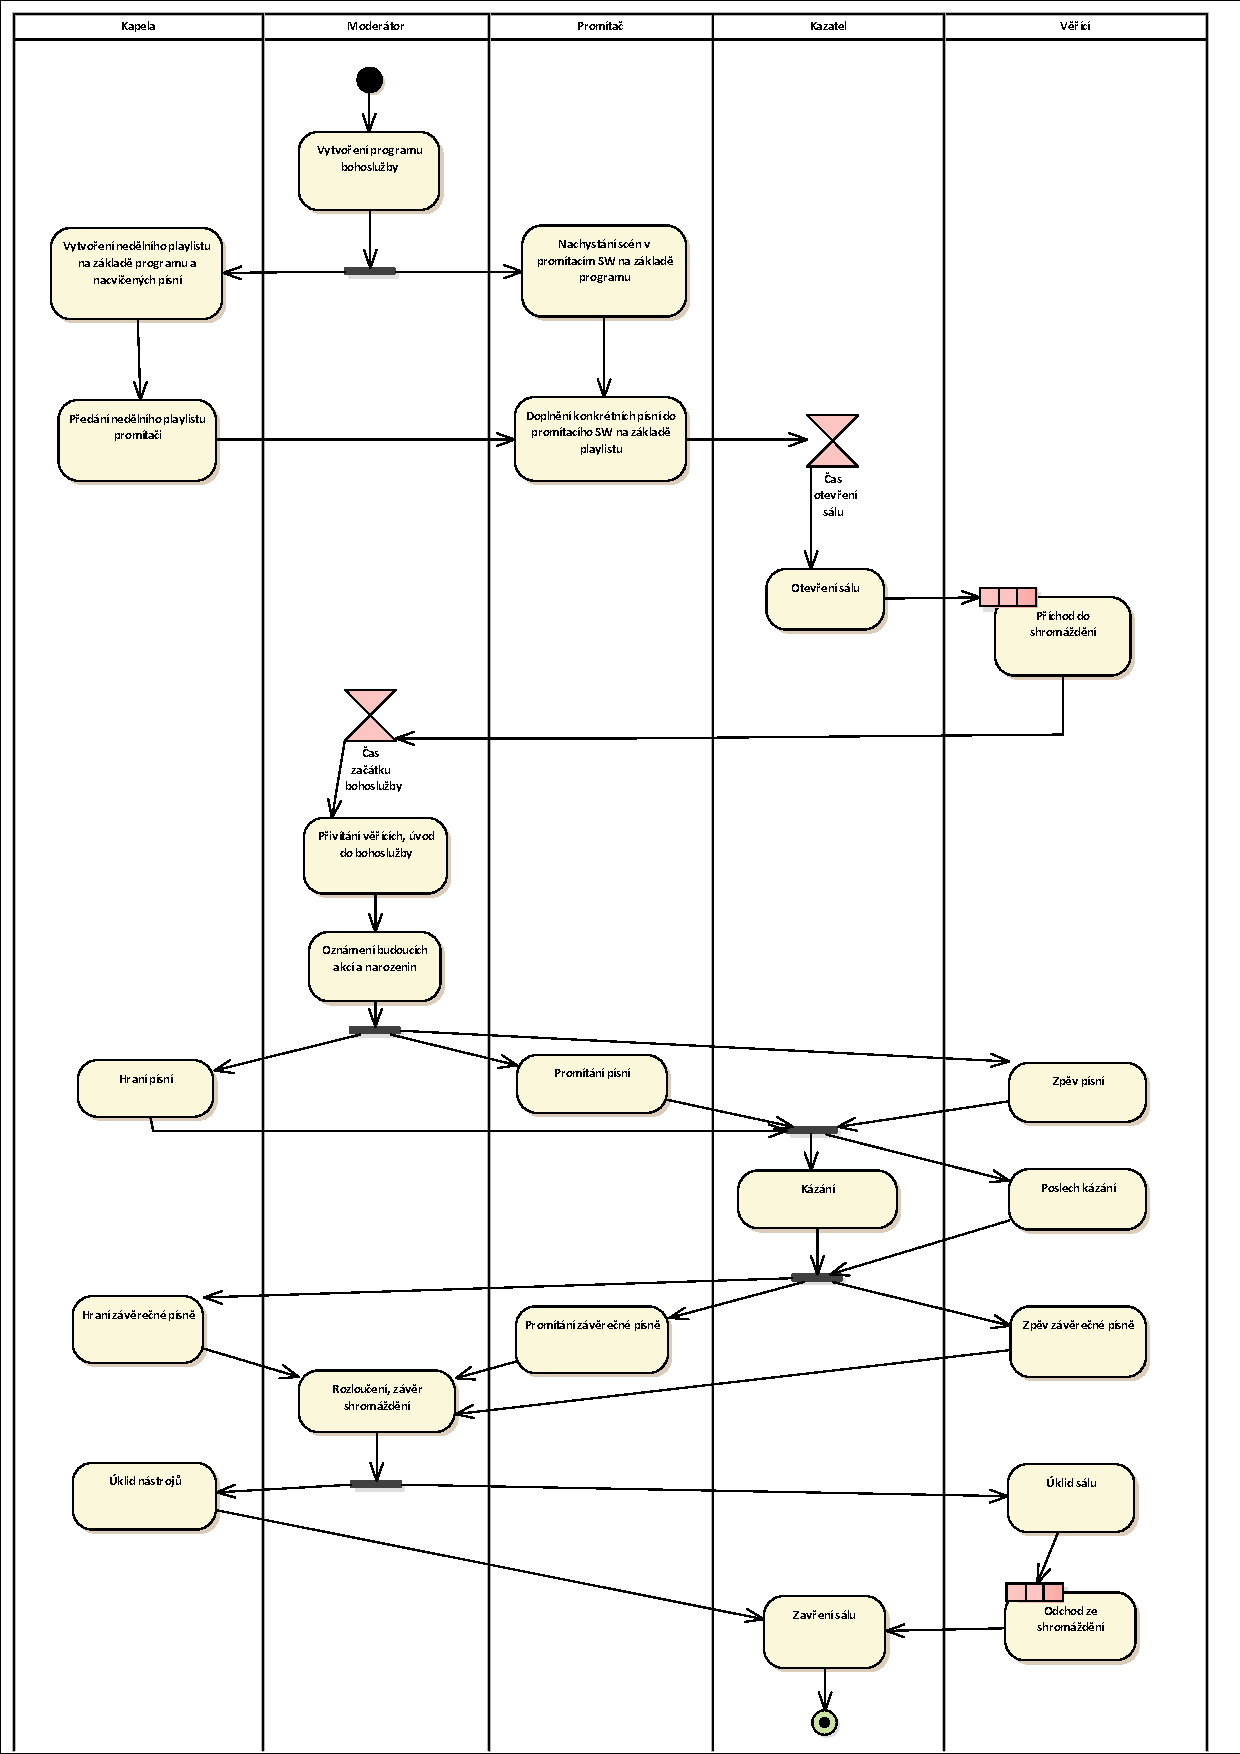
\includegraphics[width=\textwidth]{images/2-analyza/2-1-nedelni-shromazdeni.pdf}
    \caption{Diagram aktivit průběhu nedělního shromáždění}
\end{figure}

\begin{figure}
    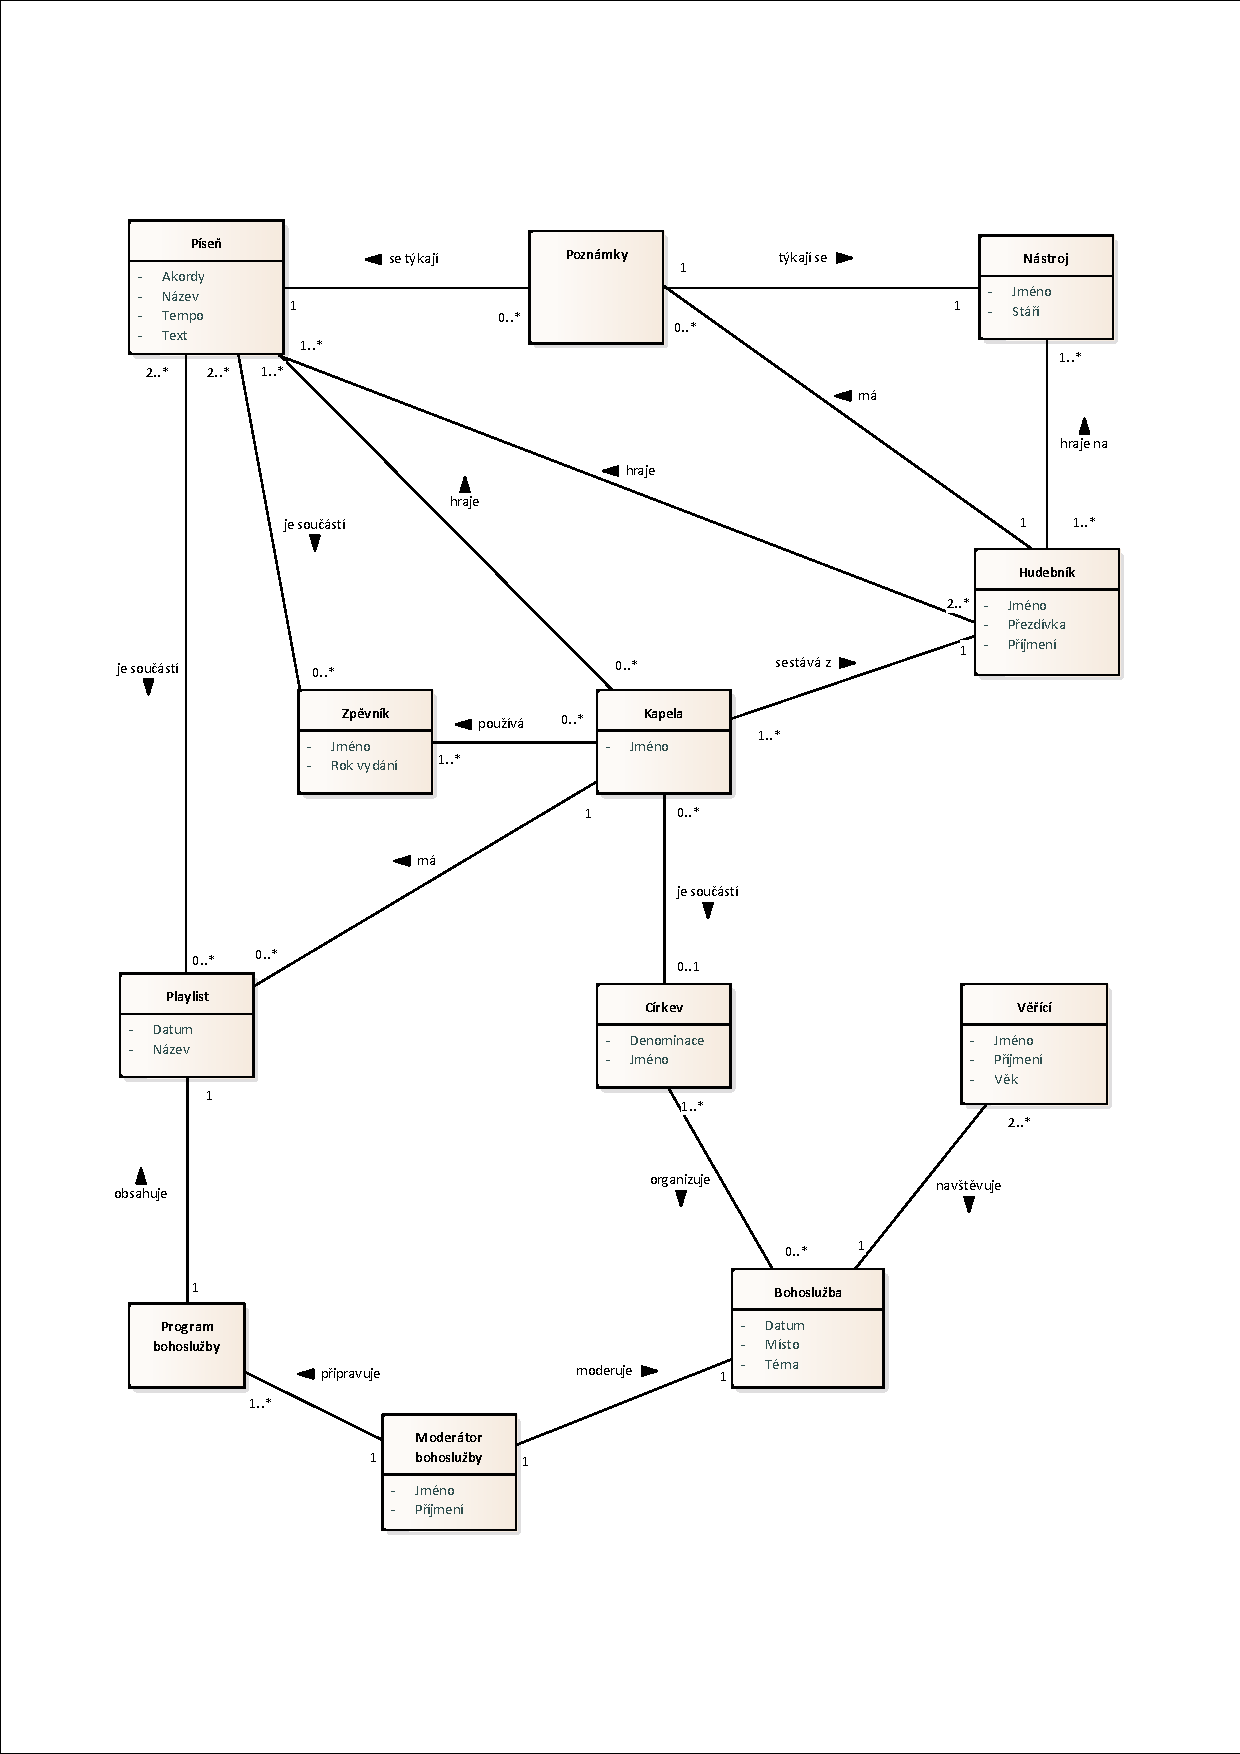
\includegraphics[width=\textwidth]{images/2-analyza/2-2-domenovy-model.pdf}
    \caption{Doménový model náboženských shromáždění}
\end{figure}

\subsection{Apoštolská církev Agapé Český Těšín}
\label{ac-agape}

Apoštolská církev Agapé Český Těšín (dále jen AC Agapé) \cite{ac-agape} se skládá z přibližně 70 členů, z~nichž třetinu tvoří Poláci. AC Agapé se schází ve staré židovské synagoze v Českém Těšíně. Synagoga je vybavena připojením k internetu, dataprojektorem a počítačem s operačním systémem Windows 10. Na bohoslužbě se běžně zpívá přibližně 10 až 15 písní. Střídají se zde dvě skupiny hudebníků -- Jóšafat a Agapebend, které čítají každá přibližně 5--10 členů. Každá skupina má svůj vlastní zpěvník o přibližně 100 písních s tím, že existují písně, které jsou v obou zpěvnících, každá skupina je ale hraje v jiném tempu, s jiným textem nebo v jiném jazyce. Zpěvníky jsem v~roce 2017 převedl do digitální podoby do formátu OpenSong \cite{open-song-format}.

Kromě nedělní bohoslužby se zde věřící scházejí také v neformálních domácích skupinách. Program domácích skupin není pevně dán, většinou je zde ale přítomen alespoň jeden hudebník, který zajistí blok 3--5 písní. Domácnosti jsou vybaveny připojením k internetu a televizí podporující technologie pro zrcadlení obrazovky. Písně jsou vybírány \uv{na přání} věřících ze zpěvníku skupiny, ze které je právě přítomný hudebník.

\subsection{Křesťanský sbor Český Těšín}
\label{krsb-tesin}

Křesťanský sbor Český Těšín (dále jen KřSb Český Těšín) \cite{krsb-tesin} se skládá z přibližně 70 členů. KřSb Český Těšín se schází ve vlastní budově zrekonstruovaného dětského centra v Českém Těšíně, která je vybavena připojením k internetu, dataprojektorem a počítačem s operačním systémem Windows 10. V průběhu bohoslužby se běžně zpívají 3 písně, kromě těchto písní se zde ale navíc vyskytuje systém \uv{podávání písní}. Každou neděli je tak kromě skupiny hudebníků určena navíc skupina klavíristů, kteří pokrývají dva zde používané zpěvníky - Písně nového života (dále jen PNŽ) a Gloria, každý čítající přibližně 500 písní. Věřící pak mají možnost z jednoho z těchto zpěvníků vybrat libovolné písně, které jsou hudebníkem zahrány, přičemž shromáždění zpívá sborově (bez sólisty u mikrofonu).

Kromě nedělní bohoslužby se v budově KřSb Český Těšín také v pátek večer setkává klub mládeže Přístav \cite{krsb-pristav}. Přístav je zaměřen na věkovou skupinu 13--19 let, od čehož se odvíjí i program setkání: začíná se hrou, následuje blok 3--4 písní, které připravuje skupina hudebníků Přístav Worship, 30 minutové zamyšlení na témata aktuální pro věkovou skupinu mladých a diskuze nad tématem spojené s konzumací jídla. Skupina Přístav Worship se skládá z 8 hudebníků a její zpěvník, čistě v digitální formě, obsahuje přibližně 30 písní.

\subsection{Křesťanský sbor Pyšely}
\label{krsb-pysely}

Křesťanský sbor Pyšely (dále jen KřSb Pyšely) \cite{krsb-pysely} se skládá z přibližně 30 členů. KřSb Pyšely se schází v budově Rodinného centra Zajíček o.s. v Zaječicích. Tato budova je vybavena připojením k internetu, není ale vybavena ani počítačem, ani dataprojektorem. Na bohoslužbě se běžně zpívá přibližně 5 písní, které má na starost jediné uskupení hudebníků, které zde působí. Zdejší hudební uskupení používá zpěvník v digitální a papírové podobě obsahující přibližně 30 písní.

\section{Funkční požadavky}

Jak jsem již nastínil v kapitole \nameref{uvod}, ve své práci se zabývám dvěma problémy, z čehož vyplývají dvě různé skupiny funkčních požadavků. Při porovnávání stávajících řešení budu tedy porovnávat zvlášť, zda systém splňuje požadavky týkající se koordinace zpěvu věřících a hudebního doprovodu (písmeno K) a požadavky týkající se přípravy písní (písmeno P).

\subsection{K1 Zobrazení textu aktuálně hrané písně}
\label{zobrazeni-textu-hrane-pisne}

Věřící v průběhu zpěvu písní potřebují vědět, kterou píseň hudební doprovod aktuálně hraje. Zkušení věřící, kteří jsou členy náboženského shromáždění dlouho, texty písní již znají, jsou tedy schopni aktuální hranou píseň rozpoznat samostatně. Nově příchozí věřící však texty písní neznají a potřebují tedy zjistit a vidět text aktuálně hrané písně.

\subsection{P1 Zobrazení seznamu písní a detailu písně}
\label{zobrazeni-seznamu-pisni-detailu}

Hudební doprovod potřebuje vidět seznam všech písní. U každé písně pak systém musí zobrazit její akordy a text včetně možnosti úpravy velikosti písma tak, aby byly text i akordy čitelné. Jelikož někteří členové hudebního doprovodu  pouze zpívají, systém by měl umožnit skrytí akordů. Pro členy hudebního doprovodu by pak měl systém poskytnout možnost nastavení transpozice akordů.

\subsection{P2 Organizace písní do zpěvníků}
\label{organizace-pisni-do-zpevniku}

Hudební doprovod potřebuje způsob, kterým zorganizuje jednotlivé písně do zpěvníků tak, aby byl schopen písně identifikovat jejich číslem ve zpěvníku a mohl ve zpěvníku efektivně vyhledávat podle tohoto čísla, případně názvu písně.

Název písně ale není spolehlivým identifikátorem. Často se stává, že různí členové hudebního doprovodu mají stejnou píseň zapamatovanou pod jiným názvem -- systém by měl tedy zvládnout také vyhledávání podle textu písně.

\subsection{P3 Správa písní a zpěvníků}
\label{sprava-pisni-zpevniku}

Hudební doprovod písně zpívané a hrané při náboženských shromážděních občas obměňuje. Přibližně jednou za 2 až 3 měsíce proběhne také přeuspořádání písní ze starých zpěvníků do~no\-vých. Systém proto musí umožnit hudebníkům úpravu, přidávání a odebírání písní a vedoucímu také vytváření, úpravu, odebírání zpěvníků a přesouvání písní mezi jednotlivými zpěvníky.

\subsection{P4 Správa playlistu}
\label{sprava-playlistu}

Z analýzy vyplynulo, že hudební doprovod pravidelně nejen na nedělní shromáždění připravuje seznam písní, které bude hrát -- playlist. Systém tak musí umožnit přidání písní do playlistu, jejich odebrání a změnu pořadí písně v rámci playlistu.

\subsection{P5 Správa členů kapely}
\label{sprava-clenu-kapely}

V systému bude působit více hudebních uskupení z různých náboženských shromáždění. Je proto nutné, aby systém umožnil každému uskupení mít oddělený zpěvník a oddělené písně, které budou přístupné pouze členům daného uskupení.

Z rozhovorů vyšel požadavek na rozdílná práva pro vedoucího, který může přidávat, upravovat a odebírat členy, zpěvníky a písně; hudebníka, který může upravovat pouze písně a zpěváka, který nemá právo upravovat.

\subsection{P6 Správa poznámek k písním}
\label{sprava-poznamek}

Členové hudebního doprovodu mají k jednotlivým písním různé poznámky. Zpěváci si k jednotlivým částem písně zaznamenávají, kde zpívají první a druhý hlas, hudebníci si naopak zaznamenávají kdy mají sólo nebo jaký použít rejstřík na svém hudebním nástroji. Tyto poznámky se vztahují pouze ke konkrétnímu členovi a ostatní členové ani vedoucí by je neměli vidět.

\subsection{P7 Synchronizace písní a zpěvníků}
\label{synchronizace-pisni-zpevniku}

Mezi členy hudebního doprovodu musí být synchronizovány jednotlivé písně a zpěvníky. Z rozhovorů s jednotlivými členy hudebních uskupení jsem zjistil, že jsou uskupení rozmanitou skupinou -- někteří členové mají zařízení s operačním systémem iOS, někteří macOS, Android a někteří mobilní zařízení ani nevlastní. Nezávisle na platformě, pro kterou bude systém vytvořen, musí systém umožnit synchronizaci písní a zpěvníků i na ostatní platformy, včetně možnosti tisku písní pro členy, kteří nevlastní žádné mobilní zařízení.

\subsection{P8 Synchronizace playlistu}
\label{synchronizace-playlistu}

Sestavený playlist musí vedoucí hudebního doprovodu před začátkem shromáždění předat jednotlivým hudebníkům. Systém musí tedy vedoucímu umožnit nahrání playlistu a jednotlivým členům hudebního doprovodu pak jeho stažení.

\section{Nefunkční požadavky}

V průběhu rozhovorů členové hudebního doprovodu vznesli také následující nefunkční požadavky na aplikaci:

\subsection{N1 Offline funkčnost (alespoň v režimu pro čtení)}
\label{offline-funkcnost}

V létě náboženská shromáždění pořádají letní tábory, které se často konají v přírodě, kde není dostupné připojení k internetu. Aplikace tak musí fungovat i bez přístupu k internetu, a to alespoň pro zobrazení playlistu, zpěvníků a písní. Úpravy bude provádět především vedoucí hudebního doprovodu, a to doma. Z průzkumu Českého statistického úřadu vyplývá, že je dnes více než 80 \% domácností připojeno k internetu. \cite{internet-usage-czechia} Podpora úprav bez připojení k internetu tak není nezbytně nutná a používání aplikace pouze zpříjemní.

\subsection{N2 Mobilní aplikace pro systémy iOS a macOS}

Vzhledem k tomu, že bude aplikace používána nejen v budovách náboženských shromáždění, ale také v domácnostech nebo v přírodě, musí se jednat o aplikaci pro mobilní telefon.

Z průzkumu mezi členy hudebního doprovodu vyplynulo, že bude nejvýhodnější aplikace pro systém iOS a macOS, jelikož právě tyto systémy používají vedoucí a více než polovina členů.

\subsection{N3 API rozhraní pro budoucí rozšířitelnost}

Z analýzy vyplývá, že v hudebních doprovodech existuje nezanedbatelné množství členů, kteří vlastní mobilní telefon s operačním systémem Android. Členové hudebních doprovodů se také zmínili o možnosti budoucího rozšíření zpěvníku do webové verze. Systém tak musí využívat API rozhraní, aby bylo toto případné budoucí rozšíření co nejjednodušší.

\subsection{N4 Přístupné a intuitivní rozhraní aplikace}

Většina členů hudebního doprovodu, tedy hlavní cílové skupiny uživatelů aplikace, je starší než 40 let. Aplikace tedy musí mít jednoduché a intuitivní rozhraní, aby se v ní vyznali i starší uživatelé, kteří nemají bohaté zkušenosti s používáním mobilních zařízení. Vzhledem k vyššímu věku některých členů hudebního doprovodu je také nutné, aby aplikace podporovala nastavení větší velikosti textu.

\subsection{N5 Podpora češtiny a polštiny}

Hudební uskupení z náboženských shromáždění, pro které je aplikace určena, jsou složena z~nezanedbatelné části také z polsky mluvících obyvatel. Aplikace tedy musí umožnit volbu jazyka a to minimálně mezi českým a polským jazykem.

\subsection{N6 Cena}

V náboženských shromážděních je obecně problém s finančním zajištěním čehokoliv. Většina služeb se tak opírá o dobrovolnost věřících. Jediný, kdo bývá placený, a to jen v některých shromážděních, je kazatel, který práci v shromáždění věnuje celý týden. Aplikace tedy musí být vytvořena zadarmo a měla by mít co nejnižší provozní náklady a náklady na údržbu.

\section{Stávající řešení koordinace zpěvu a doprovodu}

Problémy přípravy a koordinace zpěvu věřících a hudebního doprovodu náboženská shromáždění provází od jejich vzniku, z čehož vyplývá, že se o jejich řešení snaží věřící už dlouhá staletí.

Problém koordinace zpěvu věřících a hudebního doprovodu je v dnešní době řešen především třemi způsoby: Lidská paměť, Papírový zpěvník a Promítač. Tyto způsoby porovnám a zhodnotím, zda jsou pro náboženská shromáždění dostačující.

\subsection{Lidská paměť}

Velká část věřících a někteří hudebníci už znají texty a akordy jednotlivých písní nazpaměť -- při zpěvu písní tedy během prvních slov aktuálně hranou píseň poznají. Toto řešení je vhodné v~případě, kdy písní není mnoho, často se neobměňují a do náboženských shromáždění nepřichází mnoho nových věřících. Věřící také musí mít dobrou paměť, aby si texty písní pamatovali. Toto řešení z analyzovaných shromáždění používají jednotliví věřící, pro všechny ale není použitelné.

\subsection{Papírový zpěvník}

V historii nejčastěji používané řešení, od kterého se v posledních letech začíná ustupovat. Každé\-mu členu shromáždění je dán papírový zpěvník, ve kterém jsou všechny písně seřazeny podle jejich čísla ve zpěvníku. Hudební doprovod pak oznámí jméno písně, která je hrána a věřící si ji nalistují. Toto řešení je používáno ve shromáždění \nameref{krsb-pysely} a také při \uv{podávání písní} ve shromáždění \nameref{krsb-tesin}. Od řešení papírového zpěvníku se v poslední době ustupuje vzhledem k jeho vysoké ceně v případě velkého počtu věřících a také vzhledem k~obtížnosti úpravy jednou vytisknutého zpěvníku.

\subsection{Promítač}

Promítač je osoba, která promítá s pomocí dataprojektoru a promítacího programu text aktuálně hrané písně. Věřící při zpěvu písní sledují plátno, na kterém vidí text aktuálně hrané písně. V~dnešní době se jedná o nejčastěji používané řešení -- je vhodné pro libovolný počet věřících a písně v něm se dají libovolně upravovat. Jediným slabým článkem tohoto řešení je promítač samotný -- často tuto roli dostávají mladší věřící, kteří se v průběhu zpěvu písní zahledí do~mobilního telefonu a píseň zapomenou přepnout.

Na trhu jsou k dispozici různé promítací programy. Nejčastěji používaným je OpenSong. Ten umožňuje jednoduchou správu písní, organizaci do zpěvníků, správu playlistu a promítání aktuálně hrané písně. OpenSong využívá OpenSong formát \cite{open-song-format}, který je jednoduše čitelný jak lidským okem, tak strojově (jedná se o XML). OpenSong je používán ve shromáždění \nameref{ac-agape}.

Druhým nejčastěji používaným promítacím programem je OpenLP. Ten oproti OpenSongu umožňuje také promítání videí a prezentací včetně jejich zařazení do playlistu. OpenLP používá OpenLyrics formát \cite{open-lyrics-format}, který je lidsky obtížně čitelný, strojově se ale stále jedná o čitelné XML. OpenLP je používáno ve shromáždění \nameref{krsb-tesin}.

\subsection{Mobilní aplikace}

V rámci analýzy jsem také hledal mobilní aplikace, které by umožňovaly synchronizaci písní mezi hudebním doprovodem a věřícími, žádnou takovou aplikaci jsem ale nenašel. Z rozhovoru s~členy hudebního doprovodu jsem navíc zjistil, že by taková aplikace pro shromáždění ani neměla velký přínos -- někteří věřící nechtějí nebo nemůžou používat mobilní telefon a stávající řešení promítače věřícím plně vyhovuje.

\subsection{Shrnutí}

Z rozhovoru s členy hudebních uskupení v jednotlivých náboženských shromáždění vyplynulo, že jsou věřící v jednotlivých shromážděních se stávajícími řešeními koordinace zpěvu a hudebního doprovodu  spokojeni.

Při tvorbě mobilní aplikace zpěvníku pro náboženská shromáždění tedy nebudu vytvářet nová řešení problému koordinace zpěvu věřících a hudebního doprovodu, místo toho aplikaci napojím na stávající systémy, což bude řešeno ve funkčních požadavcích \nameref{sprava-playlistu} a \nameref{synchronizace-pisni-zpevniku}.

\section{Stávající řešení přípravy písní}

Problém přípravy písní je mnohem obecnější a řeší jej mnohé aplikace zpěvníku, které jsou dostupné na obchodech s aplikacemi pro operační systémy Android a iOS. Těchto řešení je velké množství, proto provedu analýzu pouze u těch, která náboženská shromáždění již používají nebo používaly a u těch řešení z obchodů s aplikacemi, které zhodnotím jako vhodné.

Pro tato řešení následně sestavím tabulku, ve které porovnám, v jaké míře splňují stanovené funkční a nefunkční požadavky.

\subsection{Papírový zpěvník}

Stejně jako u koordinace zpěvu věřících a hudebního doprovodu, i u přípravy písní je nejčastěji používaným řešením použití papírového zpěvníku. Jeho výhodou je neomezená funkčnost bez přístupu k internetu, jednoduchost a také možnost poznámek -- vytisknutý zpěvník si může hudebník bez problému popsat libovolnými poznámkami.

Papírový zpěvník ale přináší značné nevýhody -- není zde možnost úpravy textu písní nebo přidávání a odebírání písní ze zpěvníku. Příprava zpěvníku je náročná -- zpěvník musí být vytvořen, následně vytištěn a to v desítkách kusů. Pokud se hudebník rozhodne, že bude chtít hrát píseň z jiné tóniny, musí si k vytištěné písni poznamenat akordy v jiné tónině, což je v případě častých změn akordů značně nepřehledné. Náročné je také přidání nového člena -- musí se pro něj vytisknout nová kopie zpěvníku.

\subsection{Zpěvník v galerii telefonu}

Zejména mezi mladými hudebníky v náboženských shromážděních je velmi populární způsob zpěvníku ve formě sdílených fotografií na chatovací platformě. Každá konverzace odpovídá playlistu na jednu akci. Výhodou je velmi jednoduchý způsob přidání nového uživatele a správa oprávnění, nevýhodou je ale nemožnost použití takového řešení pro velký počet uživatelů a stejně jako v případě papírového zpěvníku zde chybí možnost úpravy stávajících písní nebo změny akordů v případě transpozice.

\subsection{OpenSongApp}

Aplikace OpenSongApp je dostupná na mobilní zařízení s operačním systémem Android. Umož\-ňuje jednoduchou správu písní, zpěvníků a playlistů v OpenSong formátu \cite{open-song-format}, je tedy plně kompatibilní s počítačovým promítacím programem OpenSong. Právě proto je aktivně používána v~shromáždění \nameref{ac-agape}.

Hlavní nevýhodou této aplikace je její omezení na operační systém Android. Druhou nevýho\-dou je synchronizace písní a playlistů mezi jednotlivými členy kapely a promítačem -- OpenSongApp samotná sice používá stejný formát jako OpenSong, neumožňuje ale synchronizaci samotnou. Písně je tedy třeba synchronizovat buď pomocí síťového úložiště nebo manuálně přes kabel, což je ale pro věkovou skupinu členů hudebního doprovodu často nesplnitelný úkol. OpenSongApp také neumožňuje správu uživatelů a kontrolu práv.

\subsection{Setlists}

Aplikace Setlists je dostupná pouze pro operační systém iOS. Setlists umožňuje správu playlistů a písní, její nevýhodou je vysoká cena (600 Kč na jedno zařízení), absence funkcionality zpěvníků, správy uživatelů. Rozhraní není příliš intuitivní a písně nelze jednoduše nahrát do aplikace. Toto řešení bylo jeden týden využíváno v \nameref{ac-agape}, ale příliš se neosvědčilo.

\subsection{Practice Books}

Aplikace Practice Books je dostupná pro operační systémy iOS a macOS. Umožňuje správu písní a zpěvníků a jejich synchronizaci mezi jednotlivými platformami. Její výhodou je jednoduché rozhraní a snadný způsob nahrání písní do aplikace.

Drobnou nevýhodou této aplikace je její cena, která ale není příliš vysoká -- 129 Kč na osobu. Mnohem zásadnějším problémem je ale absence playlistů, polštiny, chybějící správa členů kapely a oprávnění nebo možnost synchronizace mezi různými osobami. Aplikace také z nepochopitelných důvodů padá. Toto řešení bylo aktivně používáno v \nameref{ac-agape} během středečních domácích skupin, kdy vzhledem k tomu, že zde působil jeden hudebník nevadila absence playlistu, na nedělních shromážděních se ale příliš neosvědčila.

\subsection{Shrnutí}

Po provedení analýzy stávajících řešení jsem sepsal do tabulky, zda jednotlivá řešení splňují (A), částečně splňují (C), nesplňují (N) nebo nejsou relevantní (-) k stanoveným funkčním/nefunkčním požadavkům.

Z tabulky lze vidět, že neexistuje řešení, které by alespoň částečně splňovalo všechny funkční a nefunkční požadavky. Stávající řešení nesplňují funkční požadavek \nameref{sprava-clenu-kapely}, a velká část z nich má také problém s funkčním požadavkem \nameref{synchronizace-playlistu}.

\begin{table}[H]
\caption{Tabulka splnění funkčních požadavků stávajícími řešeními}
\begin{tabular}{|l||c|c|c|c|c|c|c|c|}
    \hline
    řešení & P1 & P2 & P3 & P4 & P5 & P6 & P7 & P8 \\
    \hline
    Papírový zpěvník           & A & A & C & C & N & A & N & N \\
    Zpěvník v galerii telefonu & N & N & N & A & A & N & C & A \\
    OpenSongApp                & A & A & A & A & N & A & C & C \\
    Setlists                   & A & N & C & A & N & N & C & C \\
    Practice Books             & A & A & A & N & N & N & C & N \\
    \hline
\end{tabular}
\end{table}

\begin{table}
\caption{Tabulka splnění nefunkčních požadavků stávajícími řešeními}
\begin{tabular}{|l||c|c|c|c|c|c|}
\hline
    řešení & N1 & N2 & N3 & N4 & N5 & N6 \\
    \hline
    Papírový zpěvník           & A & - & - & A & A & C \\
    Zpěvník v galerii telefonu & A & A & - & A & A & A \\
    OpenSongApp                & A & N & N & A & A & A \\
    Setlists                   & A & A & N & N & N & N \\
    Practice Books             & A & A & N & A & N & C \\
    \hline
\end{tabular}
\end{table}

Po domluvě s členy hudebního doprovodu v jednotlivých shromážděních jsem se tedy rozhodl implementovat mobilní aplikaci, která bude řešit problém přípravy zpěvu věřících a hudebního doprovodu. Problém koordinace zpěvu věřících a hudebního doprovodu bude nadále řešen promítačem a papírovým zpěvníkem, nově vzniklá aplikace ale s těmito řešeními bude kompatibilní.

%---------------------------------------------------------------
\chapter{Návrh}
%---------------------------------------------------------------

\begin{chapterabstract}
    V této kapitole se budu zabývat návrhem aplikace samotné. Nejprve popíšu případy užití a navrhnu architekturu aplikace, pak porovnám existující technologie pro tvorbu aplikací a vyberu tu nejvhodnější pro svou práci. V závěru pak navrhnu vhodný prototyp uživatelského rozhraní.
\end{chapterabstract}

\section{Případy užití}

Na základě provedené analýzy a jednotlivých funkčních požadavků jsem navrhl následující přípa\-dy užití:

\subsection{K1 Zobrazení textu aktuálně hrané písně}

\begin{enumerate}
    \item Věřící otevře aplikaci
    \item Aplikace zobrazí Přihlášení
    \item Věřící klikne na tlačítko \uv{Host}
    \item Aplikace zobrazí dialog Přihlášení -- kapela
    \item Věřící klikne na kapelu, jejíž aktuálně hranou píseň chce zobrazit
    \item Aplikace zobrazí Detail písně -- host
\end{enumerate}

\subsection{P1.1 Zobrazení seznamu všech písní}
\label{P1.1}

\begin{enumerate}
    \item Člen kapely otevře aplikaci
    \item Aplikace zobrazí Přihlášení
    \item Člen kapely stiskne tlačítko Přihlásit přes Apple
    \item Aplikace zobrazí dialog pro přihlášení přes Apple
    \begin{enumerate}
        \item Přihlášení bylo neúspěšné \emph{(uživatel přihlašování zamítl, nemá platný Apple účet)} -- aplikace zobrazí chybovou hlášku s možností zkusit přihlašování znovu
        \item Přihlášení bylo úspěšné -- aplikace zobrazí Seznam písní
    \end{enumerate}
\end{enumerate}

\subsection{P1.1.1 Filtrování seznamu všech písní}
\label{P1.1.1}

\begin{enumerate}
    \item Člen kapely postupuje podle scénáře \hyperref[P1.1]{P1.1}
    \item Člen kapely stiskne tlačítko Filtrovat
    \item Aplikace ukáže Seznam písní -- filtr
    \item Člen kapely vybere v zaškrtávacím seznamu jména zpěvníků, které chce zobrazit, případně stiskne tlačítko Zobrazit/skrýt vše
    \item Aplikace zobrazí v seznamu písní pouze písně z vyfiltrovaných zpěvníků
\end{enumerate}

\subsection{P1.1.2 Hledání v seznamu všech písní}
\label{P1.1.2}

\begin{enumerate}
    \item Člen kapely postupuje podle scénáře \hyperref[P1.1]{P1.1}
    \item Člen kapely zadá do vyhledávacího pole název, číslo, nebo text písně
    \item Aplikace zobrazí v seznamu písní pouze písně, které vyhovují zadanému číslu, názvu nebo textu
\end{enumerate}

\subsection{P1.2 Zobrazení detailu libovolné písně}

\begin{enumerate}
    \item Člen kapely postupuje dle scénáře \hyperref[P1.1]{P1.1}
    \item Člen kapely klikne na jméno písně, jejíž detail (text, akordy a poznámky) chce zobrazit
    \item Aplikace zobrazí Detail písně
\end{enumerate}

\subsection{P2 Zobrazení seznamu všech písní ve zpěvníku}
\label{P2}

\begin{enumerate}
    \item Člen kapely postupuje podle scénáře \hyperref[P1.1]{P1.1}
    \item Člen kapely stiskne šipku u jména zpěvníku, ze kterého chce zobrazit všechny písně
    \item Aplikace zobrazí Detail zpěvníku
\end{enumerate}

\begin{figure}
    \subsection{P3.2 + P6 Správa písní}
    \label{P3.2 + P6}
    \centering
    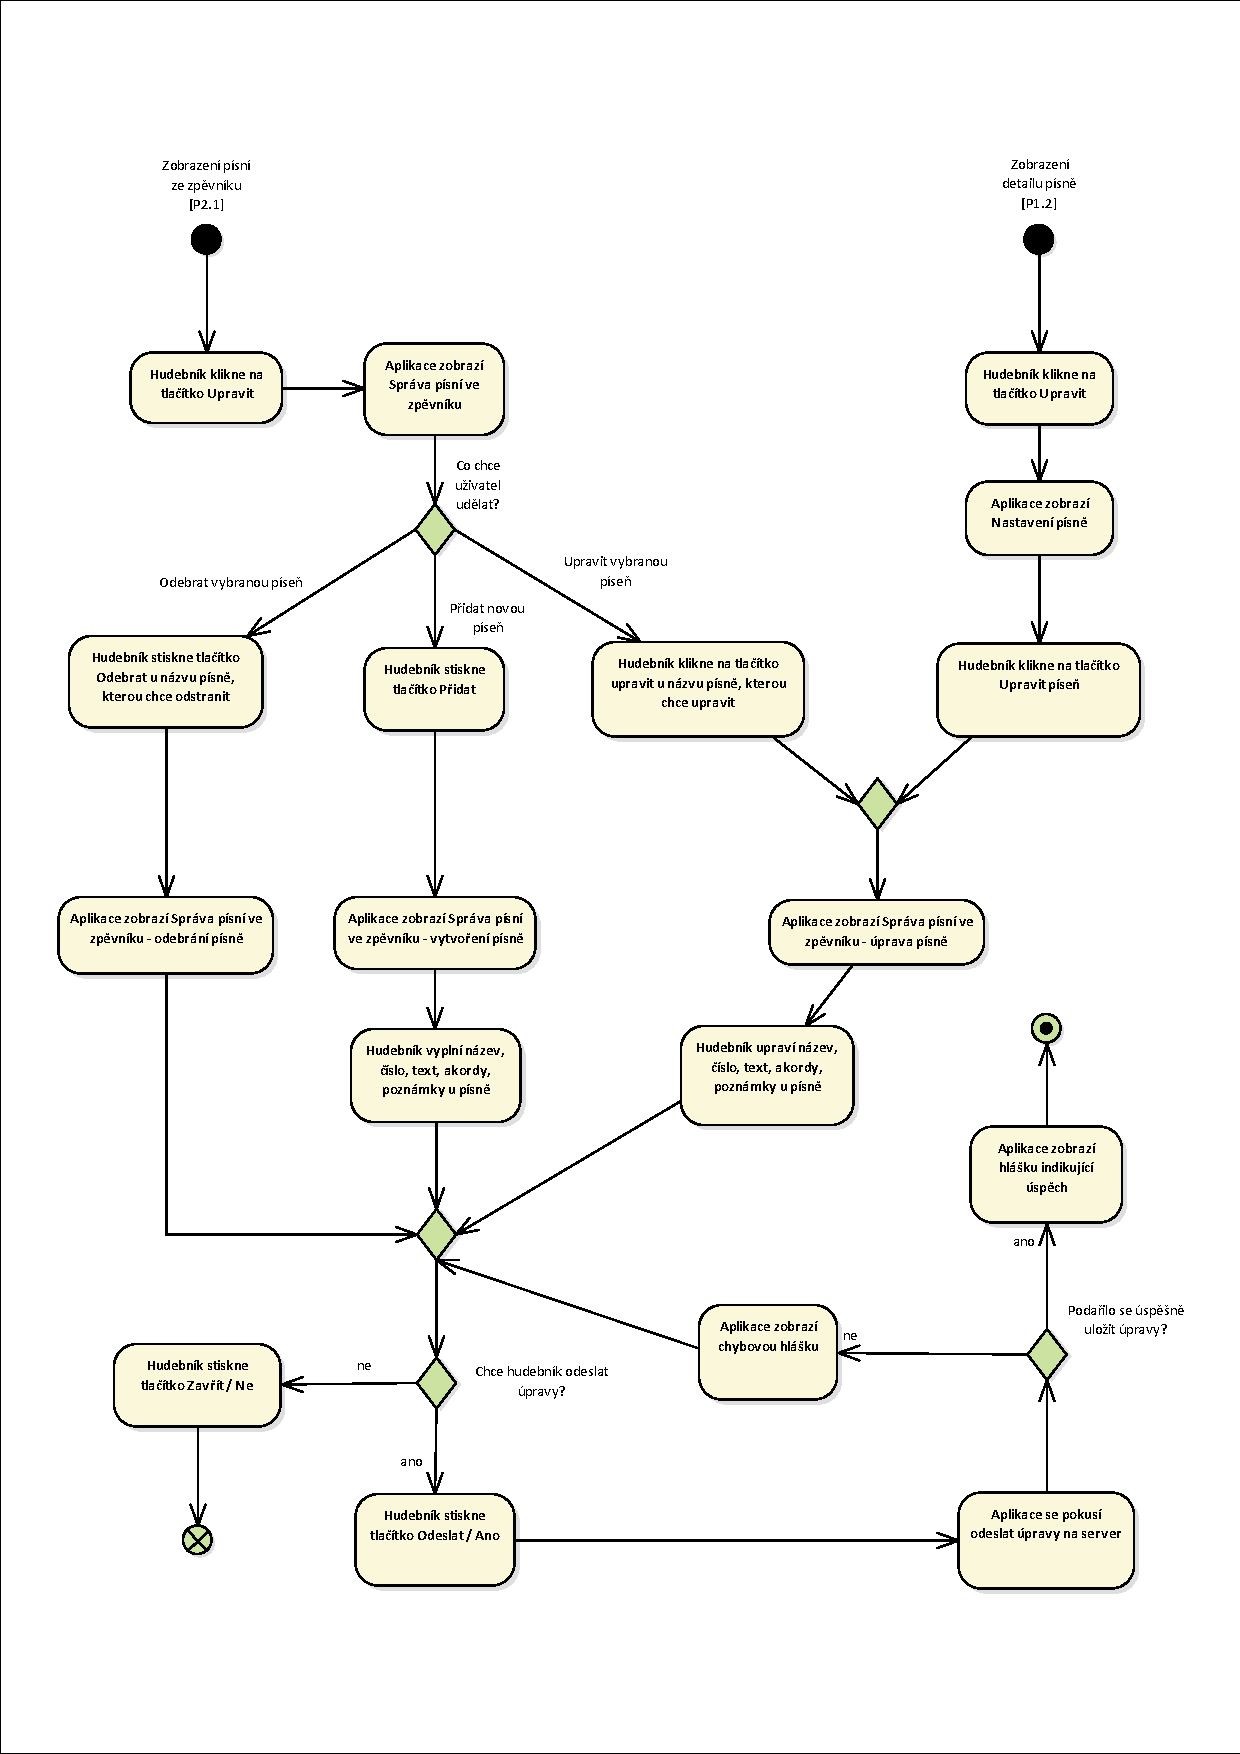
\includegraphics[width=\textwidth-8pt]{images/3-navrh/3-1-uc-sprava-pisni.pdf}
    \caption[Diagram případů užití Správa písní a Správa poznámek k písni]{Správa písní -- přidání nové písně, úprava a odebrání písně}
\end{figure}

\subsection{P3.1 Přidání nového zpěvníku}
\label{P3.1}

\begin{enumerate}
    \item Vedoucí postupuje dle scénáře \hyperref[P1.1]{P1.1}
    \item Vedoucí stiskne tlačítko Upravit
    \item Aplikace zobrazí Správa playlistů a zpěvníků
    \item Vedoucí stiskne tlačítko Přidat
    \item Aplikace zobrazí dialog Správa playlistu a zpěvníků - nový zpěvník
    \item Vedoucí vyplní informace o zpěvníku
    \item \begin{enumerate}
        \item Vedoucí chce přidat nový zpěvník -- stiskne Odeslat
        \item Vedoucí nechce přidat nový zpěvník -- stiskne Zavřít
    \end{enumerate}
    \item \begin{enumerate}
        \item Aplikace odešle žádost o vytvoření zpěvníku na server
        \item Aplikace zavře dialogové okno
    \end{enumerate}
    \item \begin{enumerate}
        \item \begin{enumerate}
            \item Vytvoření zpěvníku se podaří -- aplikace zobrazí dialog o úspěchu
	    \item Vytvoření zpěvníku je neúspěšné -- aplikace zobrazí chybový dialog
        \end{enumerate}
    \end{enumerate}
\end{enumerate}

\subsection{P3.3 Úprava zpěvníku}
\label{P3.3}

\begin{enumerate}
    \item Vedoucí postupuje dle bodu 1--3 scénáře \hyperref[P3.1]{P3.1}
    \item Vedoucí stiskne tlačítko Upravit u názvu zpěvníku, který chce upravit
    \item Aplikace zobrazí dialog Správa playlistu a zpěvníků - úprava zpěvníku
    \item Vedoucí vyplní nové informace o zpěvníku
    \item \begin{enumerate}
        \item Vedoucí chce upravit zpěvník -- stiskne Odeslat
        \item Vedoucí nechce upravit zpěvník -- stiskne Zavřít
    \end{enumerate}
    \item \begin{enumerate}
        \item Aplikace odešle žádost o úpravu zpěvníku na server
        \item Aplikace zavře dialogové okno
    \end{enumerate}
    \item \begin{enumerate}
        \item \begin{enumerate}
            \item Úprava zpěvníku se podaří -- aplikace zobrazí dialog o úspěchu
	    \item Úprava zpěvníku je neúspěšná -- aplikace zobrazí chybový dialog
        \end{enumerate}
    \end{enumerate}
\end{enumerate}

\subsection{P3.4 Odebrání zpěvníku}
\label{P3.4}

\begin{enumerate}
    \item Vedoucí postupuje podle bodu 1--3 scénáře \hyperref[P3.1]{P3.1}
    \item Vedoucí stiskne tlačítko Odebrat u názvu zpěvníku, který chce odebrat
    \item Aplikace zobrazí dialog Správa playlistu a zpěvníků - odebrání zpěvníku
    \item \begin{enumerate}
        \item Vedoucí chce odebrat zpěvník -- stiskne Ano
	\item Vedoucí nechce odebrat zpěvník -- stiskne Ne
    \end{enumerate}
    \item \begin{enumerate}
        \item Aplikace odešle žádost o odebrání zpěvníku na server
	\item Aplikace zavře dialogové okno
    \end{enumerate}
    \item \begin{enumerate}
        \item \begin{enumerate}
            \item Odebrání zpěvníku se podaří -- aplikace zobrazí dialog o úspěchu
	    \item Odebrání zpěvníku je neúspěšné -- aplikace zobrazí chybový dialog
        \end{enumerate}
    \end{enumerate}
\end{enumerate}

\subsection{P4.1 Přidání libovolné písně do playlistu}
\label{P4.1}

Přidat píseň do playlistu lze dvěma způsoby -- scénář 1 je optimalizován pro přidání jedné písně, pro případ přidávání více písní je optimalizován scénář 2.

\subsubsection{P4.1.1 Přidání jedné písně do playlistu}
\label{P4.1.1}

\begin{enumerate}
    \item Člen kapely postupuje dle scénáře \hyperref[P1.1]{P1.1}
    \item Člen kapely dlouze podrží prst na názvu písně, kterou chce exportovat k tisku
    \item Aplikace zobrazí Seznam písní -- kontextová nabídka
    \item Člen kapely vybere z kontextové nabídky možnost Přidat do playlistu
    \item Aplikace přidá danou píseň na konec playlistu
\end{enumerate}

\subsubsection{P4.1.2 Přidání více písní do playlistu}
\label{P4.1.2}

\begin{enumerate}
    \item Člen kapely postupuje dle scénáře \hyperref[P1.1]{P1.1}
    \item Člen kapely stiskne tlačítko Upravit
    \item Aplikace zobrazí Správa playlistu a zpěvníků
    \item Člen kapely stiskne tlačítko Přidat u názvu písní, které chce přidat do playlistu
    \item Aplikace přidá dané píseň na konec playlistu
\end{enumerate}

\subsection{P4.2 Úprava pořadí písní v playlistu}
\label{P4.2}

\begin{enumerate}
    \item Člen kapely postupuje dle scénáře \hyperref[P4.1.1]{P4.1.1}
    \item Člen kapely potáhne píseň z playlistu na požadovanou pozici v rámci playlistu
    \item Aplikace provede požadovanou změnu pořadí písní v playlistu
\end{enumerate}

\subsection{P4.3 Odebrání libovolné písně z playlistu}
\label{P4.3}

Odebrání písně z playlistu je stejně jako u přidávání písní do playlistu možné dvěma způsoby, kdy scénář 1 je optimalizován pro odebírání jedné písně a scénář 2 pro odebírání více písní.

\subsubsection{P4.3.1 Odebrání jedné písně z playlistu}
\label{P4.3.1}

\begin{enumerate}
    \item Člen kapely postupuje dle scénáře \hyperref[P1.1]{P1.1}
    \item Člen kapely potáhne doleva název písně, kterou chce odebrat z playlistu
    \item Aplikace odebere píseň z playlistu
\end{enumerate}

\subsubsection{P4.3.2 Odebrání více písní z playlistu}
\label{P4.3.2}

\begin{enumerate}
    \item Člen kapely postupuje dle bodu 1--3 scénáře \hyperref[P4.1.2]{P4.1.2}
    \item Člen kapely stiskne Odebrat u názvu písní, které chce odebrat z playlistu
    \item Aplikace odebere požadované písně z playlistu
\end{enumerate}

\subsection{P5.1 Zobrazení detailu kapely}
\label{P5.1}

\begin{enumerate}
    \item Člen kapely postupuje podle scénáře \hyperref[P1.1]{P1.1}
    \item Člen kapely klikne na Nastavení
    \item Aplikace zobrazí Nastavení
    \item Člen kapely vybere kapelu, jejíž detail chce zobrazit
    \item Aplikace zobrazí Nastavení -- detail kapely
\end{enumerate}

\begin{figure}
    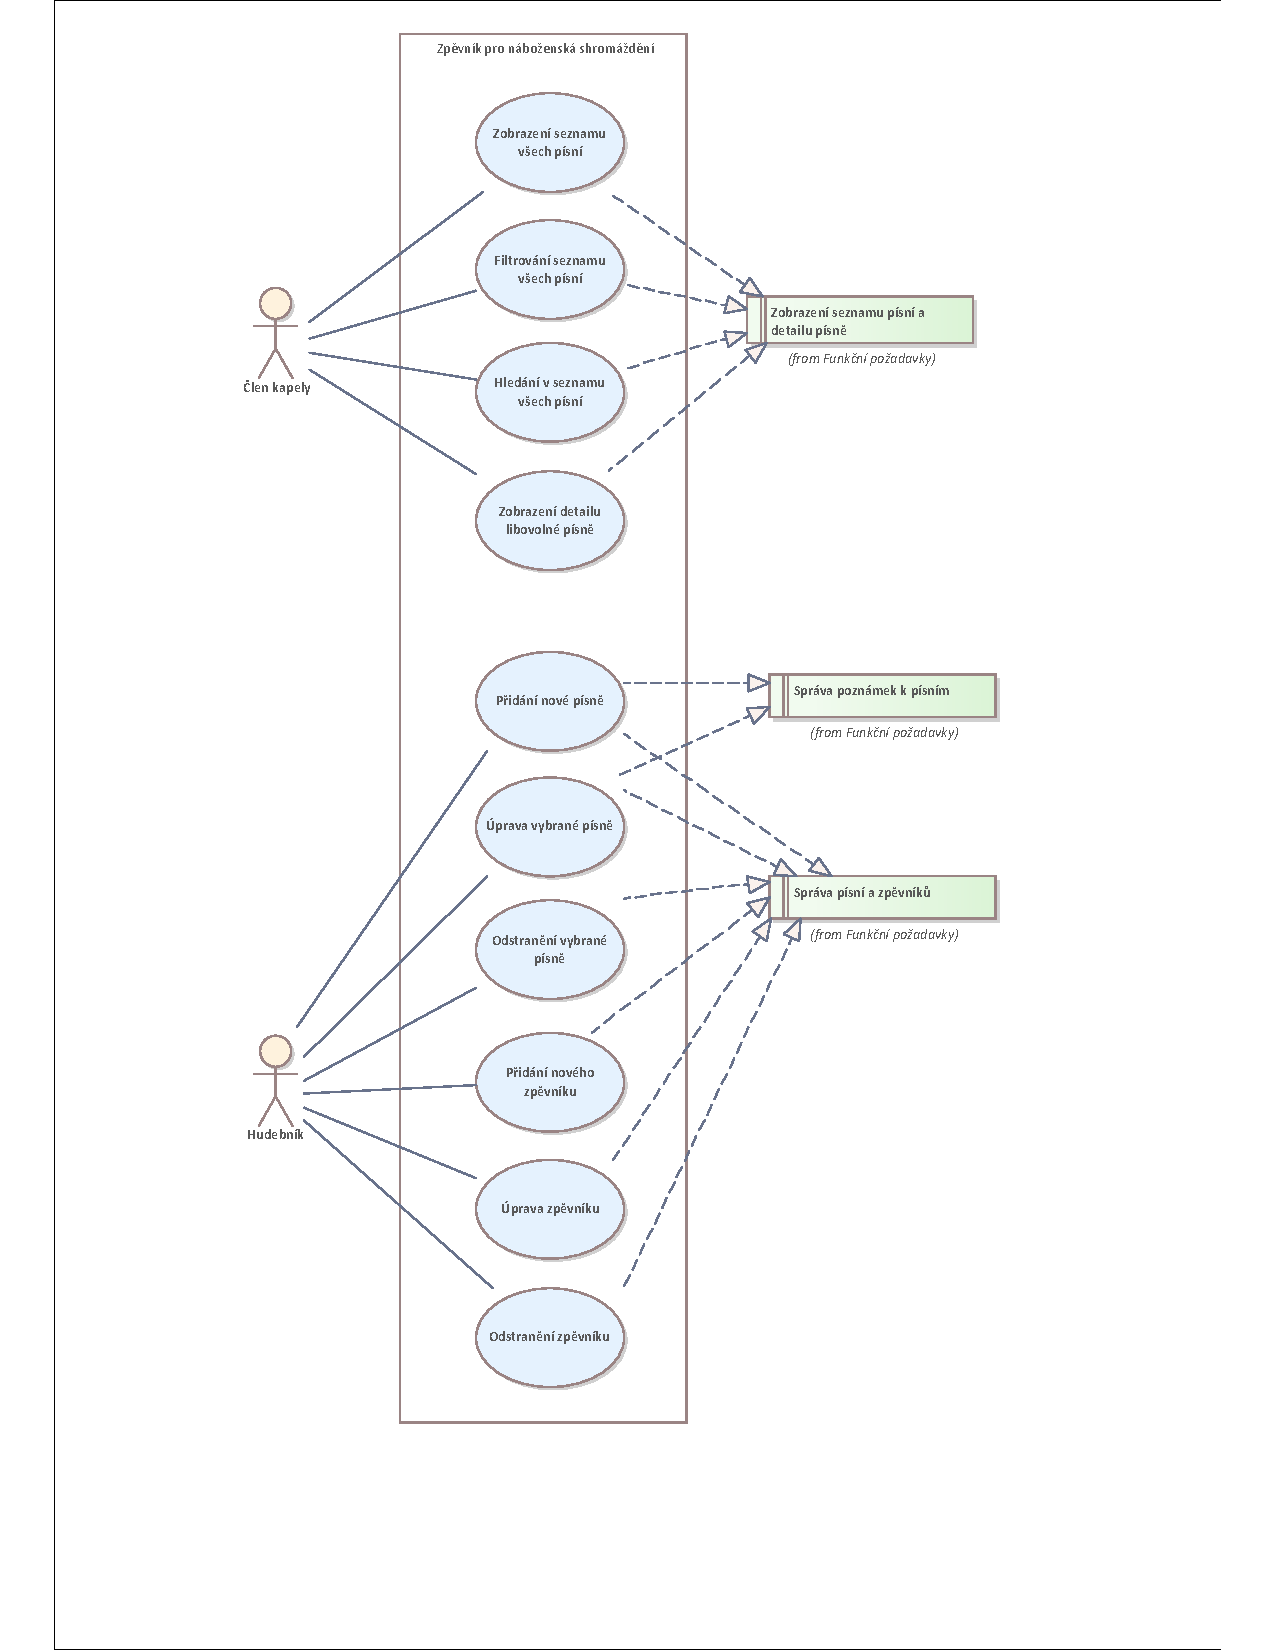
\includegraphics[width=\textwidth]{images/3-navrh/3-2-uc-model-1.pdf}
    \caption{Model případů užití -- člen kapely a hudebník}
\end{figure}

\begin{figure}
    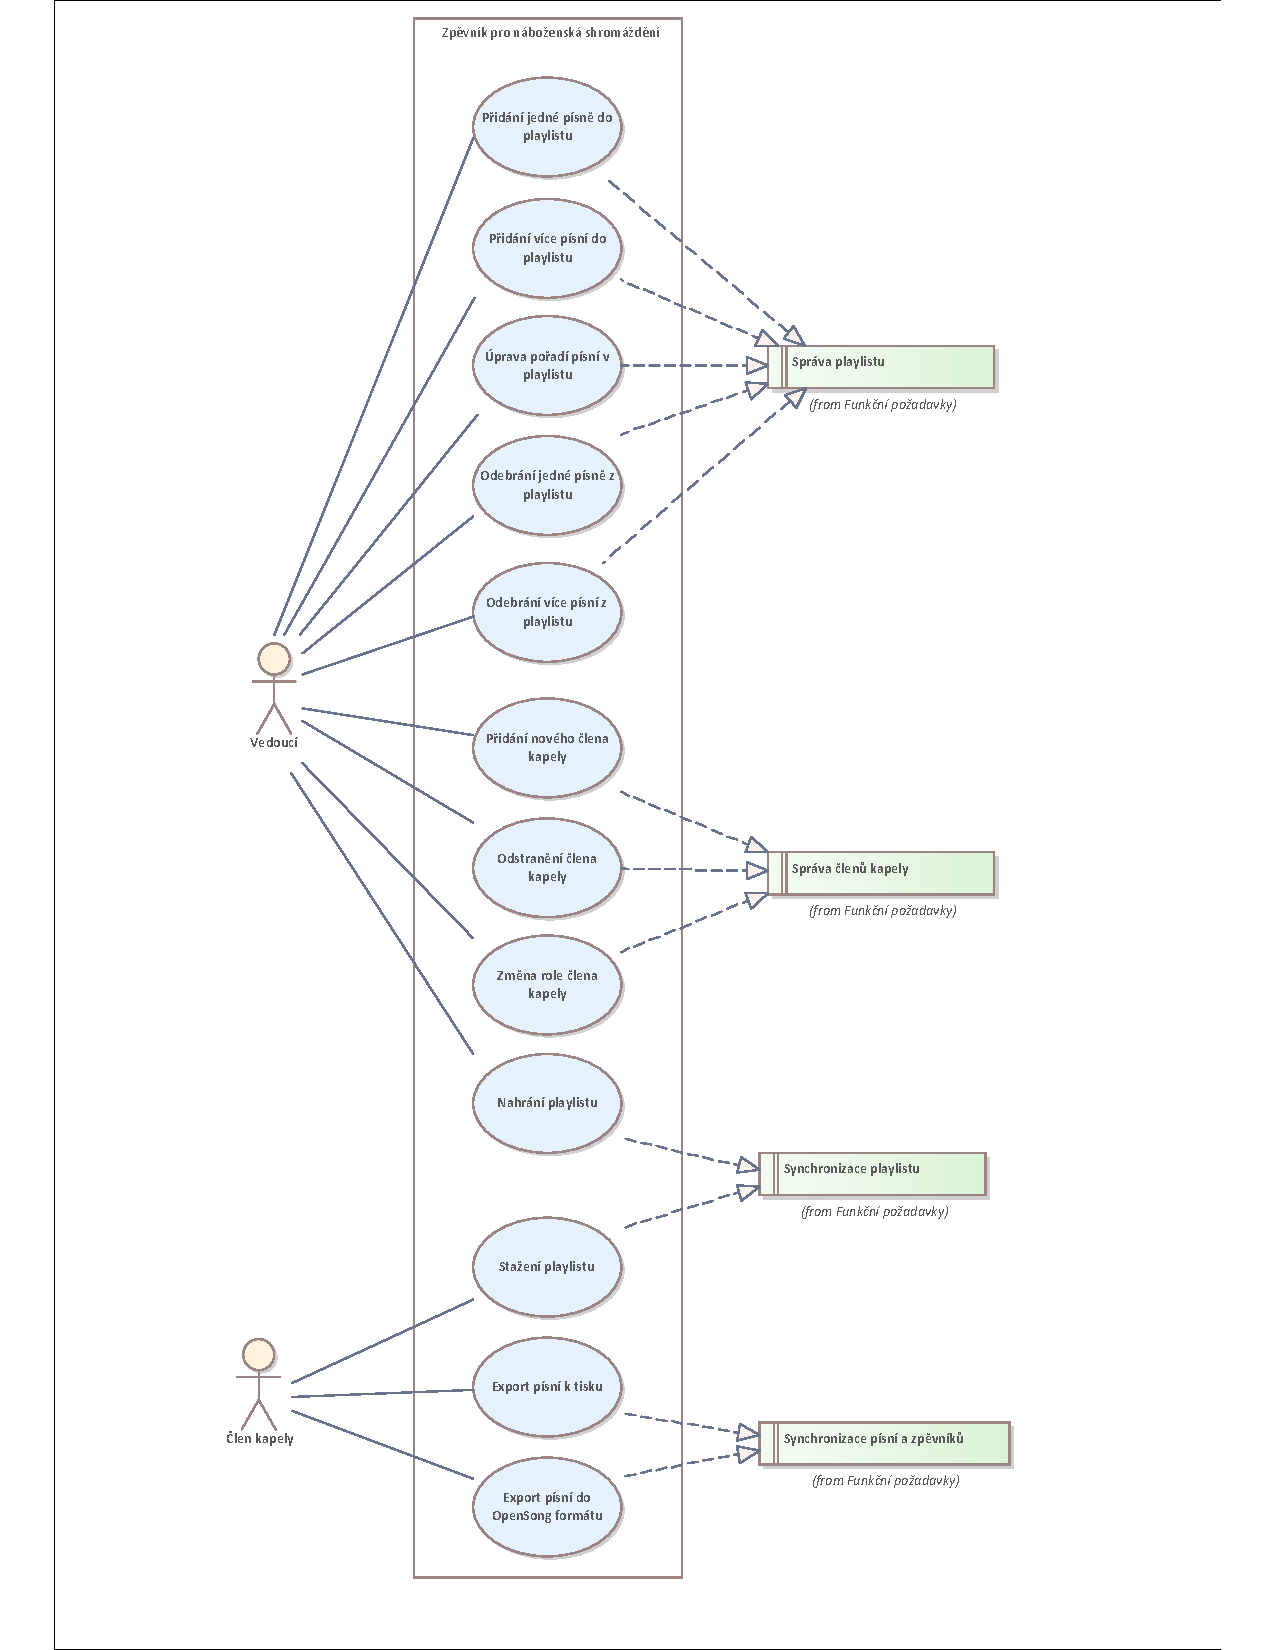
\includegraphics[width=\textwidth]{images/3-navrh/3-3-uc-model-2.pdf}
    \caption{Model případů užití -- vedoucí a člen kapely}
\end{figure}

\subsection{P5.2 Přidání nového člena kapely}
\label{P5.2}

\begin{enumerate}
    \item Vedoucí postupuje podle scénáře \hyperref[P5.1]{P5.1}
    \item Vedoucí klikne na tlačítko Upravit
    \item Aplikace zobrazí Nastavení -- správa kapely
    \item Vedoucí klikne na tlačítko Přidat
    \item Aplikace zobrazí dialog Nastavení -- nový člen kapely
    \item Vedoucí vyplní údaje nového člena
    \item \begin{enumerate}
        \item Vedoucí nového člena chce přidat -- stiskne Odeslat
        \item Vedoucí nového člena nechce přidat -- stiskne Zavřít
    \end{enumerate}
    \item \begin{enumerate}
        \item Aplikace odešle žádost o přidání nového člena
        \item Aplikace zavře dialogové okno
    \end{enumerate}
    \item \begin{enumerate}
        \item \begin{enumerate}
            \item Přidání člena se podaří -- aplikace zobrazí dialog s informací o úspěchu
            \item Přidání člena je neúspěšné -- aplikace zobrazí chybový dialog
        \end{enumerate}
    \end{enumerate}
\end{enumerate}

\subsection{P5.3 Odebrání člena kapely}
\label{P5.3}

\begin{enumerate}
    \item Vedoucí postupuje podle bodu 1--3 scénáře \hyperref[P5.2]{P5.2}
    \item Vedoucí klikne na Odebrat u člena kapely, kterého chce odebrat
    \item Aplikace zobrazí dialog Nastavení - odebrání člena kapely
    \item \begin{enumerate}
        \item Vedoucí člena chce odebrat -- stiskne Ano
        \item Vedoucí člena nechce odebrat -- stiskne Ne
    \end{enumerate}
    \item \begin{enumerate}
        \item Aplikace odešle žádost o odebrání člena
        \item Aplikace zavře dialogové okno
    \end{enumerate}
    \item \begin{enumerate}
        \item \begin{enumerate}
            \item Odebrání člena se podaří -- aplikace zobrazí dialog s informací o úspěchu
            \item Odebrání člena je neúspěšné -- aplikace zobrazí chybový dialog
        \end{enumerate}
    \end{enumerate}
\end{enumerate}

\subsection{P5.4 Změna role člena kapely}
\label{P5.4}

\begin{enumerate}
    \item Vedoucí postupuje podle bodu 1--3 scénáře \hyperref[P5.2]{P5.2}
    \item Vedoucí klikne na Zvýšit oprávnění nebo Snížit oprávnění u člena kapely, kterému chce změnit roli
    \item Aplikace zobrazí dialog Nastavení - změna role člena kapely
    \item \begin{enumerate}
        \item Vedoucí členovi chce změnit roli -- stiskne Ano
        \item Vedoucí členovi nechce změnit roli -- stiskne Ne
    \end{enumerate}
    \item \begin{enumerate}
        \item Aplikace odešle žádost o změnu role
        \item Aplikace zavře dialogové okno
    \end{enumerate}
    \item \begin{enumerate}
        \item \begin{enumerate}
            \item Změna role se podaří -- aplikace zobrazí dialog s informací o úspěchu
            \item Změna role je neúspěšná -- aplikace zobrazí chybový dialog
        \end{enumerate}
    \end{enumerate}
\end{enumerate}

\subsection{P7.1 Export písní k tisku}
\label{P7.1}

\begin{enumerate}
    \item Člen kapely postupuje dle scénáře \hyperref[P1.1]{P1.1}
    \item Člen kapely dlouze podrží prst na názvu písně, kterou chce exportovat k tisku
    \item Aplikace zobrazí Seznam písní -- kontextová nabídka
    \item Člen kapely vybere z kontextové nabídky možnost Exportovat k tisku
    \item Aplikace otevře prohlížeč se stránkou s vygenerovaným textem k tisku
\end{enumerate}

\subsection{P7.2 Export písní do OpenSong formátu}
\label{P7.2}

\begin{enumerate}
    \item Člen kapely postupuje podle bodu 1--2 scénáře \hyperref[P7.1]{P7.1}
    \item Člen kapely vybere z kontextové nabídky možnost Exportovat do OpenSong
    \item Aplikace otevře prohlížeč se stránkou s vygenerovanou písní v OpenSong formátu
\end{enumerate}

\subsection{P8.1 Nahrání playlistu}
\label{P8.1}

\begin{enumerate}
    \item Vedoucí postupuje podle scénáře \hyperref[P1.1]{P1.1}
    \item Vedoucí stiskne tlačítko Nahrát u nadpisu Playlist
    \item Aplikace zobrazí Správa playlistu a zpěvníků - výběr kapely
    \item Vedoucí vybere kapelu, do které chce nahrát playlist
    \item Aplikace se pokusí odeslat playlist na server
    \item \begin{enumerate}
        \item Playlist se nepodařilo uložit -- aplikace zobrazí chybovou hlášku
        \item Playlist se podaří uložit -- aplikace zobrazí hlášku o úspěšném uložení
    \end{enumerate}
\end{enumerate}

\subsection{P8.2 Stažení playlistu}
\label{P8.2}

\begin{enumerate}
    \item Člen kapely postupuje podle scénáře \hyperref[P1.1]{P1.1}
    \item Člen kapely stiskne tlačítko Stáhnout u nadpisu Playlist
    \item Aplikace zobrazí Správa playlistu a zpěvníků - výběr kapely
    \item Člen kapely vybere kapelu, ze které chce stáhnout playlist
    \item Aplikace se pokusí stáhnout playlist ze serveru
    \item \begin{enumerate}
        \item Playlist se nepodařilo stáhnout -- aplikace zobrazí chybovou hlášku
        \item Playlist se podaří stáhnout -- aplikace zobrazí hlášku o úspěšném uložení
    \end{enumerate}
\end{enumerate}

\section{Architektura aplikace}

Jelikož většina členů hudebního doprovodu aktivně používá zařízení s operačním systémem iOS nebo macOS, vznikl na aplikaci nefunkční požadavek na podporu těchto platforem. Vzhledem k možnému budoucímu rozšíření na další mobilní platformy nebo na web vznikl také nefunkční požadavek na API rozhraní. Na základě těchto dvou nefunkčních požadavků jsem se rozhodl aplikaci koncipovat jako multiplatformní klientskou aplikaci pro operační systém iOS a macOS a podpůrný server poskytující API rozhraní. V aplikaci budu také ukládat písně, zpěvníky a uživatele, budu tedy potřebovat databázi, se kterou bude server komunikovat.

\begin{figure}
    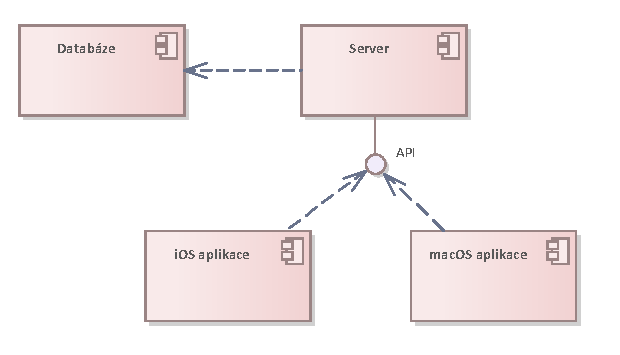
\includegraphics[width=\textwidth]{images/3-navrh/3-4-diagram-komponent.pdf}
    \caption[Diagram komponent aplikace]{Diagram komponent -- Databáze, server, API, iOS a macOS aplikace}
\end{figure}

\section{Databáze}

Existuje více způsobů, kterými může aplikace ukládat data. Jednotlivé způsoby se liší v rychlosti a efektivitě ukládání dat, v typu ukládaných dat a na základě dotazů, které budou nad daty prováděny. Tyto způsoby porovnám, a zvolím nejvhodnější pro svou aplikaci.

\subsection{Operační paměť}

Data aplikace můžou být uložena přímo v operační paměti. Toto řešení je vhodné pro dočasná data, které nemusí přežít restart aplikace. Výhodou operační paměti je také rychlost získání takto uložených dat. Pro ukládání zpěvníků, písní a dat uživatelů operační paměť nebude vhodné řešení, jelikož potřebuji, aby tato data přežila restart aplikace.

\subsection{Soubory}

Jednou z možností je ukládat data do souboru. Data do souboru můžeme ukládat v různých nestrukturovaných či strukturovaných formátech.

\begin{figure}[H]
    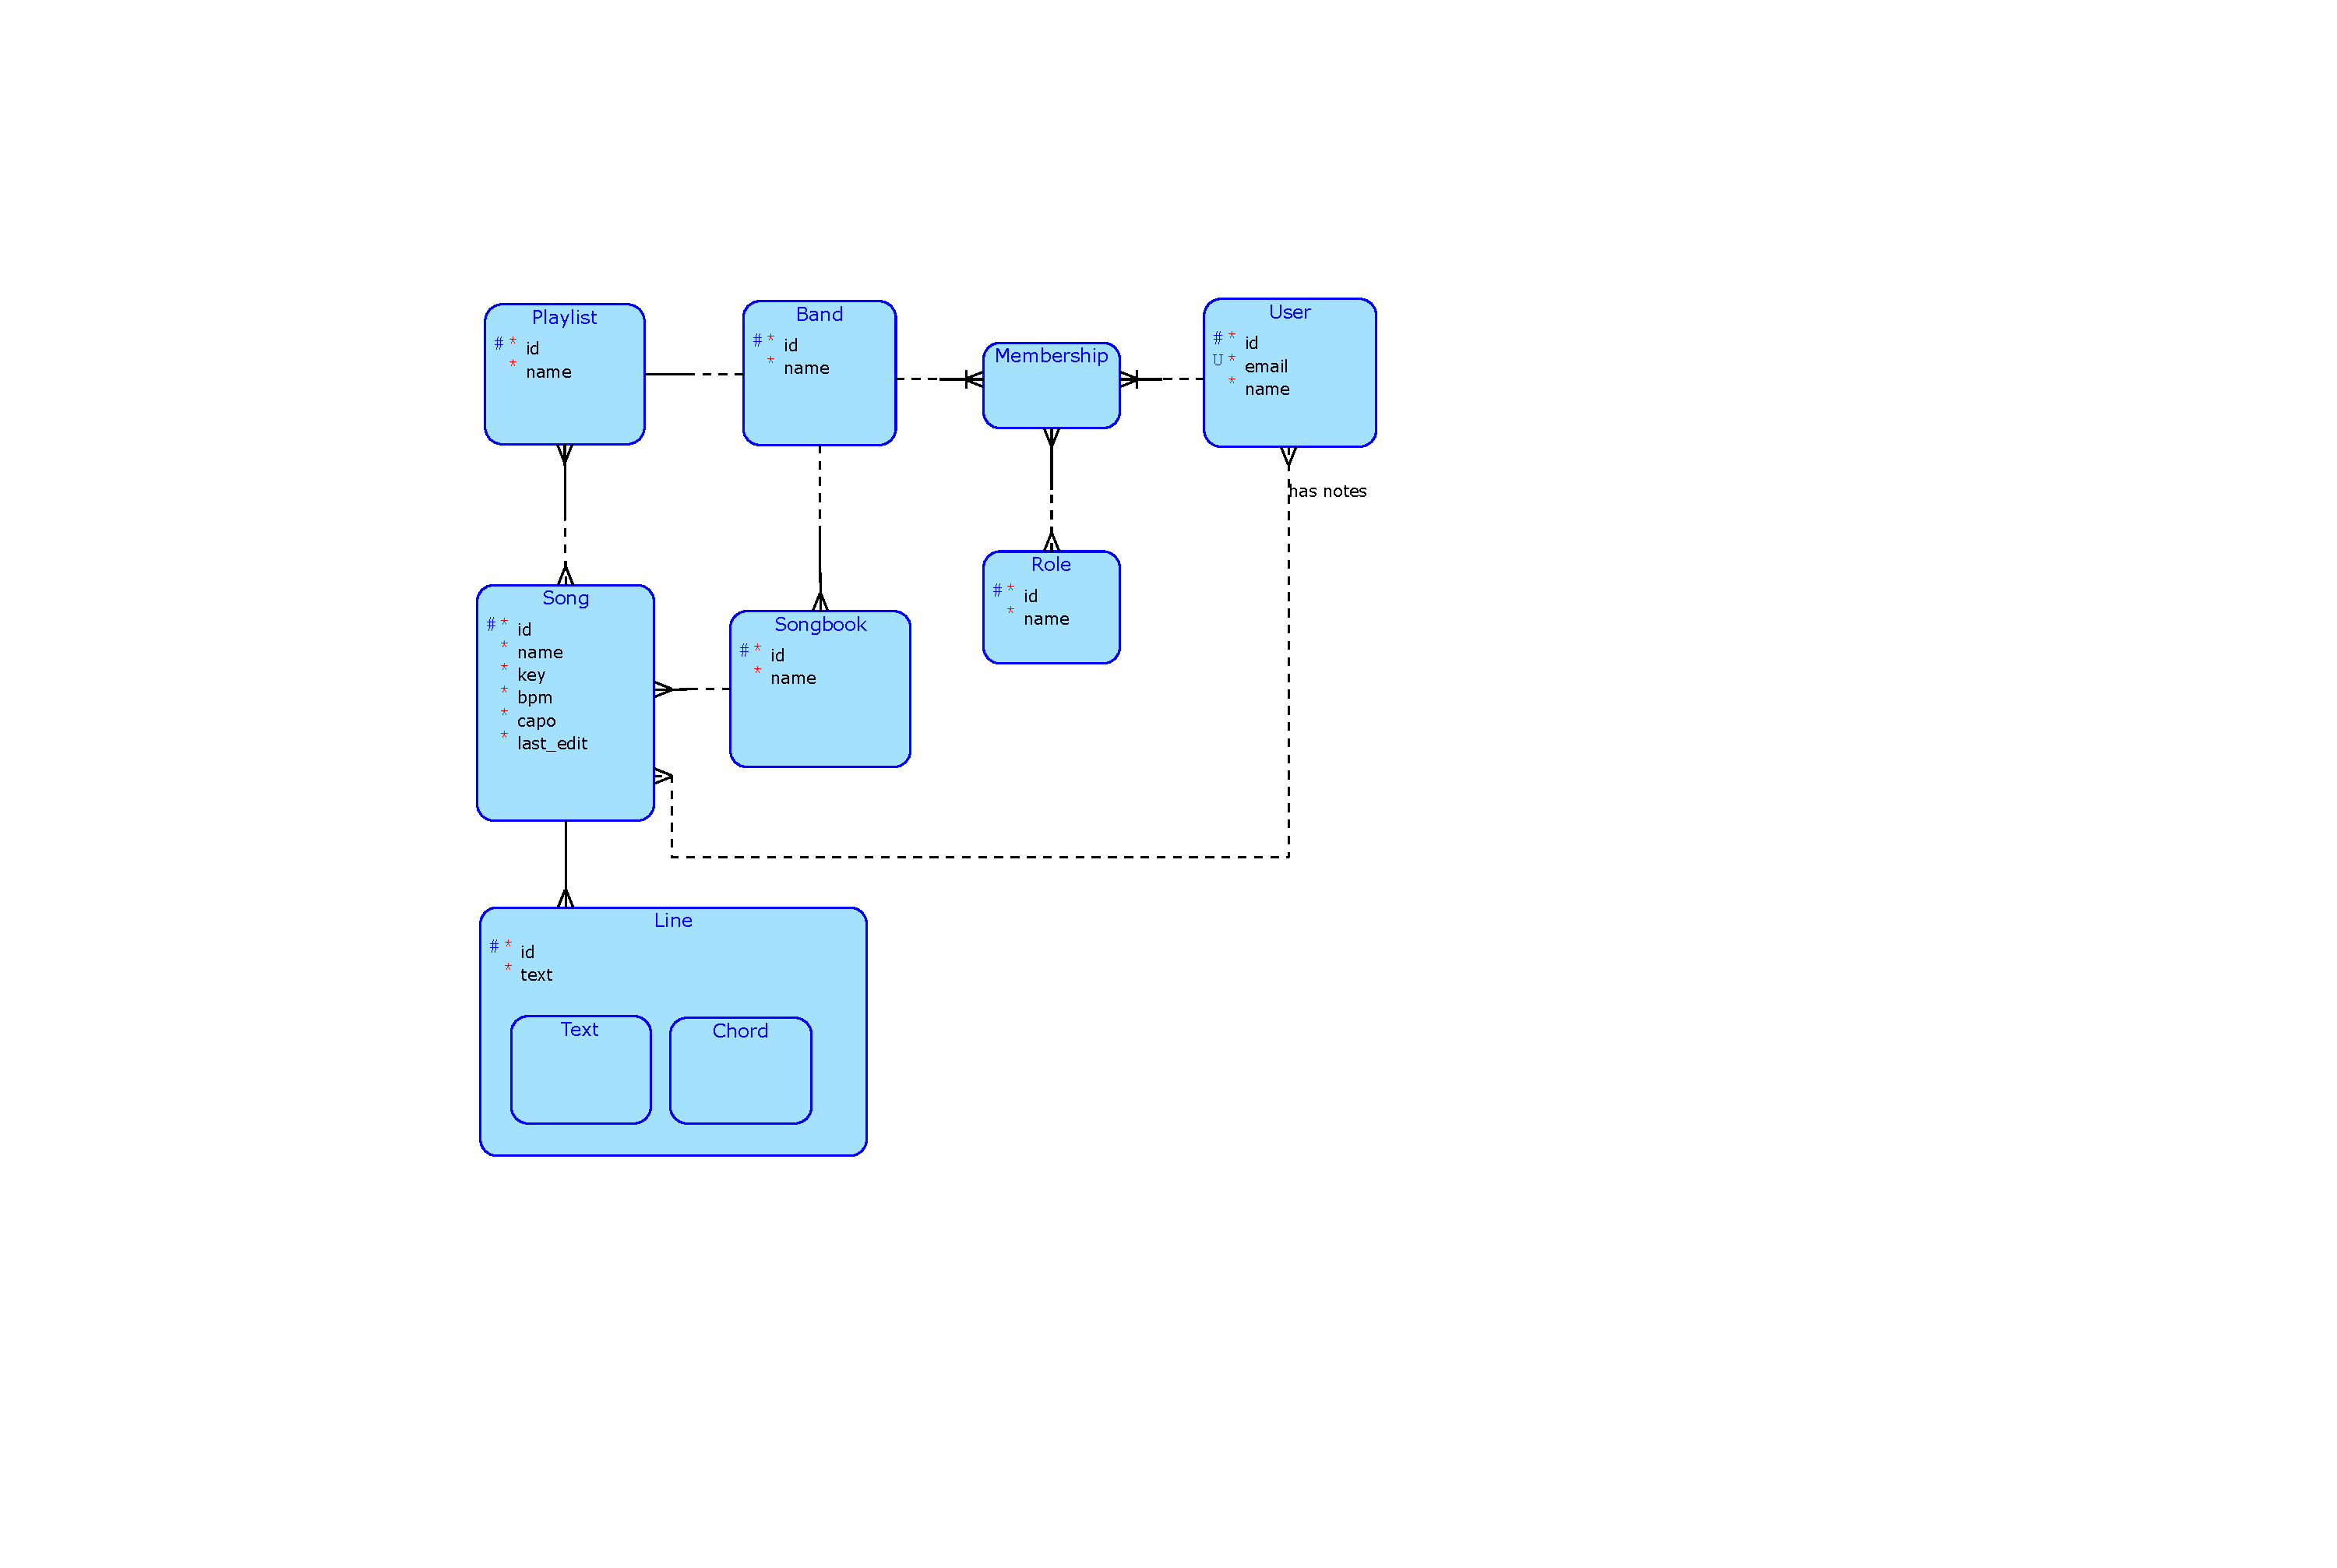
\includegraphics[width=\textwidth]{images/3-navrh/3-5-konceptualni-model.pdf}
    \caption{Konceptuální model aplikace}
\end{figure}

Nevýhodou tohoto způsobu ukládání dat je nutnost řešení problému souběžného zápisu, v~případě většího množství ukládaných dat je pak vyhledávání v datech pomalé a neefektivní. Tento způsob je vhodný pro ukládání binárních dat, jako jsou obrázky a videa. Pro data aplikace toto řešení taktéž nebude vhodné, jelikož aplikaci může používat více uživatelů najednou, a v~takovém případě by u práce se soubory mohl nastat problém při souběžném zápisu.

\subsection{Relační databáze}

Relační databáze jsou v dnešním době jedním z nejpoužívanějších řešení ukládání dat. Řeší problém souběžného zápisu a umožňují strukturované uložení dat, nad kterými lze vybudovat indexy pro rychlejší vyhledávání. \cite{what-is-rdbms}

Nevýhodou relačních databází je problematické ukládání velkého množství dat nebo binárních souborů, jako jsou obrázky a videa. Práce s daty v relační databázi je rychlá a jednoduchá díky dotazovacímu jazyku SQL. Relační databáze splňuje všechny požadavky pro uložení dat aplikace.

\subsection{NoSQL databáze}

Tradiční relační databáze byly navrženy ještě před vznikem internetu a mobilních aplikací tak, aby běžely na jediném, vertikálně škálovatelném serveru -- jedinou možností zvětšení výkonu byla koupě lepšího procesoru a paměti. NoSQL databáze umožňují horizontální škálování -- výkon je navýšen koupením většího počtu méně výkonných serverů. Oproti tradičním relačním databázím pak mají NoSQL databáze typicky volnější datové schéma a jelikož jsou informace uloženy na~více serverech, dochází k jejich duplicitám. \cite{why-nosql} O datech aplikace vím, že písní budou maximálně tisíce a uživatelů budou desítky -- nebudu tedy potřebovat databázi škálovat. Při práci s daty v~aplikaci navíc potřebuji, aby byla data aktuální a přesná.

\subsection{Zvolená databáze}

Po porovnání existujících technologií ukládání dat jsem dospěl k závěru, že pro mou aplikaci bude nejvhodnější data ukládat do relační databáze. Mezi nejčastěji používané relační databáze patří MySQL \cite{mysql}, MariaDB \cite{mariadb}, PostgreSQL \cite{postgresql}, Oracle Database \cite{oracle} a Microsoft SQL Database \cite{mssql}. Poslední dvě jmenovaná řešení, Oracle Database a Microsoft SQL Database jsou komerční řešení, ostatní opensource. Komerční řešení by byla pro účely mé bakalářské práce zbytečně příliš komplexní a drahá, rozhodl jsem se proto pro opensource řešení. Mezi MySQL, MariaDB a PostgreSQL jsem se rozhodl pro MySQL, jelikož již vlastním server s MySQL databází, který pro účely bakalářské práce můžu využít bez nutnosti nastavování nového serveru a také proto, že mám s tímto řešením největší zkušenosti.

\section{Architektura API}

API, z anglického Application Programming Interface, je mostem mezi více oddělenými aplikacemi. Architektura API je určena významem a podobou zpráv, které je API schopno zpracovávat. V průběhu let byly vytvořeny různé styly API architektury, kde každý z nich má vlastní schéma výměny dat. Diskuze, která architektura je nejlepší, tak nemá konec. \cite{altexsoft}

\subsection{SOAP}

SOAP, z anglického Simple Object Access Protocol, zpřístupňuje data v XML (eXtended Markup Language) formátu a je silně standardizovaný. Byl vytvořen Microsoftem v roce 1999. SOAP zpráva se skládá z počáteční a koncové značky, těla s požadavkem nebo odpovědí, nepovinné hlavičky a informací o případných chybách. SOAP API je napsáno v WSDL (Web Service Description Language) popisem endpointů (= adresa, se kterou lze komunikovat) a popisem všech akcí, které lze provést. Výhodou SOAPu je jeho nezávislost na platformě a programovacím jazyce, vestavěné zpracování chyb a různá bezpečnostní rozšíření -- proto se často používá pro přenos dat u bank a korporátů. Velkou nevýhodou je nutnost použití XML, která způsobuje, že přenášené datové zprávy jsou velké. \cite{altexsoft}

Jedním z problémů použití architektury SOAP pro mou aplikaci je velikost přenášených dat, kdy u mobilních aplikací platí, že čím méně dat aplikace potřebuje, tím lépe. Využití SOAP by tak mohlo způsobit vysokou datovou spotřebu aplikace a zhoršení uživatelského zážitku. Z~hlediska programování by pak byl návrh SOAP API časově zbytečně velmi náročný, což není nutné vzhledem k tomu, že na systém není požadavek na vysokou bezpečnost.

\subsection{REST}

REST, z anglického REpresentational State Transfer, je samopopisná architektura API pocháze\-jící z roku 2000. REST podporuje různé formáty, nejčastěji XML a JSON. REST není silně standardizovaný, musí ale splňovat určité požadavky, mezi které patří architektura klient-server, umožňující nezávislý vývoj jak klienta, tak serveru a bezestavovost, kdy veškerá data potřebná k zpracování požadavku jsou obsažena v požadavku samotném, sever tedy nemusí ukládat dodatečná data.

Komunikace s REST API probíhá pomocí volání endpointů, které reprezentují jednotlivé zdroje. Operace s těmito zdroji jsou pak prováděny pomocí metod protokolu HTTP. Velkou výhodou RESTu je jeho samopopisnost, kdy při použití HATEOAS (Hypertext As The Engine of Application State) je u každého požadavku uvedena sada metadat odkazujících na informace, jak API používat. Nevýhodou použití HATEOAS je ale hodně metadat, která způsobují, že zprávy jsou velké. \cite{altexsoft}

Datový formát JSON je nativně podporován většinou programovacích jazyků pro tvorbu mobilních aplikací. Při vypnutí HATEOAS navíc aplikace nebude mít vysokou datovou spotřebu. Návrh a naprogramování REST API je pak časově méně náročné než například návrh a naprogramování SOAP API.

\subsection{GraphQL}

GraphQL \cite{graphql} je architektura umožňující provedení přesného požadavku. Použití GraphQL je vhodné, pokud data obsahují hodně komplexních entit, které se k sobě vztahují. Návrh GraphQL spočívá ve vytvoření schématu všech dotazů, které lze provést a všech datových typů, které můžou být vráceny v odpovědi. To zajišťuje, že server dokáže na požadavek vždy odpovědět a data jsou vrácena přesně v podobě, která je požadována. Nevýhodou je ale složitost zachování požadavků a také množství práce před začátkem vývoje. \cite{altexsoft}

Programovací jazyky pro tvorbu mobilních aplikací GraphQL nativně nepodporují, pro jeho použití je potřeba využít externí knihovnu, jakou je například Apollo GraphQL \cite{apollo-graphql}. Aplikace navíc nebude potřebovat provádět komplexní dotazy a použití GraphQL by bylo časově náročnější než použití REST.

\subsection{Zvolená architektura}

Na základě analýzy existujících řešení pro architekturu API jsem se rozhodl si vybrat architekturu REST, která nejlépe odpovídá požadavkům -- nedochází zde k velkému objemu přenášených zpráv, návrh je v porovnání s ostatními architekturami nejméně náročný a architektura REST je nativně podporována většinou programovacích jazyků pro psaní mobilních aplikací.

\section{Návrh REST API}

Z konceptuálního modelu vyplývá, že jednotlivé zdroje budou uživatel (/user), kapela (/band), zpěvník (/songbook) a píseň (/song).

\subsection{Zdroj /user}

Na uživateli bude přístupný zdroj POST /user/login, který umožní přihlášení uživatele na základě e-mailu a hesla nebo přihlašovacího klíče. Pokud se do systému pokusí přihlásit neexistující uživatel, bude mu vytvořena nová kapela, ve které bude nastaven jako vedoucí.

\subsection{Zdroj /band}

Systém umožní získat seznam všech kapel (GET /), včetně jejich členů a rolí. Kapely následně půjde také vytvářet (POST /), upravovat (PATCH /id) a také mazat (DELETE /id).

Nad kapelou bude možné přidávat členy (POST /id/members). API také umožní jednotlivým členům (/id/members/memberId) měnit role (PATCH) nebo členy z kapely odebrat (DELETE).

Každá kapela bude mít svůj playlist (/id/playlist), který půjde získat (GET) a také nahradit (PUT).

\subsection{Zdroje /songbook a /song}

Systém umožní získat seznam všech zpěvníků, včetně písní v nich obsažených (GET /songbook). Zpěvníky umožní také vytvářet (POST /songbook), upravovat (PATCH /songbook/id) a mazat (DELETE /songbook/id).

Systém umožní také přidávání písní (POST /song), jejich úpravu (PATCH /song/id), odebrá\-ní (DELETE /song/id) a nastavení poznámek k písni (PUT /songbook/songBookId/songs/song\allowbreak{}Id/notes).

\section{Architektura serveru}

Pro server jsem zvolil třívrstvou architekturu MVC (Model View Controller). Na datové vrstvě se nachází balíčky Entity a Repository, které mají na starost získávání dat z databáze. V business vrstvě se nachází balíčky DTO a Service, které zpracovávají logiku aplikace. V prezentační vrstvě se pak nachází balíček Controller, který poskytuje navrhnuté API rozhraní.

\section{Technologie pro server}

REST API, které jsem navrhnul, poběží na serveru s pomocí jedné z možných technologií. Výběr technologie závisí většinou na zvoleném programovacím jazyce. U každého z programovacích jazyků tak porovnám dostupné technologie podle následujících kritérií: cena, vhodnost, náročnost a moje zkušenost. Podle těchto kritérií pak určím nejvhodnější technologii, s pomocí které server naimplementuji.

\subsection{PHP}
\label{symfony}

PHP \cite{php} je dynamicky typovaný programovací jazyk určen primárně pro vývoj webových aplikací. Existují v něm různé frameworky, s jejichž pomocí lze navrhnout REST API, ať už se jedná o Slim \cite{slim}, Nette \cite{nette} nebo Symfony \cite{symfony}. PHP je možné spustit na většině webových hostingů za cenu (včetně domény) do tisíce korun ročně v konfiguraci s dostatečným výkonem. Nasazení na~takový webový hosting je otázkou několika minut, kdy stačí webovou aplikaci na~hosting pouze nahrát. S programovacím jazykem PHP mám dlouholeté zkušenosti, o konkrétních technologiích mám pouze základní povědomí.

\subsection{C\#}
\label{asp-net}

C\# \cite{csharp} je staticky typovaný programovací jazyk. Je v něm napsán framework ASP.NET \cite{dotnet}, který umožňuje mimo klasické webové aplikace také návrh REST API. Jedná se o řešení zaměřené na firmy, které je úzce integrované s operačním systémem Windows. Nasazení je možné na~virtu\-ální stroj, který se včetně domény dá pořídit také do tisíce korun ročně. Nasazení je ale časově náročnější, jelikož je zde nutnost nastavení vývojového prostředí a balíčků na virtuálním stroji. S programovacím jazykem C\# ani frameworkem ASP.NET nemám žádné zkušenosti.

\subsection{Java a Kotlin}

Java \cite{java} je staticky typovaný programovací jazyk, ve kterém je napsán framework Spring Web \cite{spring-web} umožňující tvorbu webových aplikací. Nasazení je taktéž možné na virtuální stroj, platí zde tedy z hlediska ceny a obtížnosti nasazení totéž, co u \hyperref[asp-net]{ASP.NET}. S frameworkem Spring Web mám bohaté zkušenosti z bakalářského studia, kdy jsem jej využil pro tvorbu semestrálních prací v předmětech Technologie Java a Softwarové inženýrství.

Kotlin \cite{kotlin} je nový programovací jazyk od firmy Jetbrains, který běží na Java Virtual Machine. Je v něm napsán nový webový framework Ktor \cite{ktor}, který ale prozatím není ještě doladěný a nemám s ním mnoho zkušeností. Pro Ktor také není dostupná tak rozsáhlá podpora jako u~technologií typu \hyperref[symfony]{Symfony} nebo Spring Web, které jsou hojně využívané.

Kotlin běží v Java Virtual Machine, což jej činí plně kompatibilním s veškerými knihovnami napsanými v programovacím jazyce Java, a to včetně frameworku Spring Web. Kotlin je mnohem modernější jazyk, ve kterém se díky bohatým rozšířením dá napsat kód mnohem snadněji a srozumitelněji než v Javě. Proto jsem v předmětu Programování v Kotlinu naprogramoval nadstavbu nad Kotlin verzí frameworku Spring Web, která umožňuje velmi rychlé a efektivní vytvoření REST API.

\subsection{Zvolená technologie}

Na základě provedené analýzy jsem dospěl k závěru, že nejvhodnější technologií bude framework Spring Web s použitím mé nadstavby v programovacím jazyce Kotlin, a to na základě přívětivé ceny, dlouholetých zkušeností s tímto frameworkem a programovacím jazykem a rozsáhlého množství dostupných knihoven v jazycích Kotlin i Java.

\section{Architektura mobilní aplikace}

Pro vývoj aplikací pro iOS a macOS se dnes využívá už pouze programovací jazyk Swift \cite{swift}, který nahradil původní programovací jazyk Objective C. Pro tvorbu aplikace lze využít dvě architektury -- Model View Controller (MVC) a Model View ViewModel (MVVM). \cite{mvc-mvvm}

\subsection{MVC}

Architektura MVC (Model View Controller) se skládá ze tří balíčků -- Model, což jsou pouze datové struktury bez jakékoliv logiky, View obsahující definici a popis vzhledu aplikace a Controller, který řeší veškerou logiku a komunikuje s jednotlivými View. \cite{mvc-mvvm} Nevýhodou této architektury je právě fakt, že Controller obsahuje jak business, tak prezentační logiku, a dochází tedy k velkým a nepřehledným Controllerům.

\subsection{MVVM}

Architektura MVVM (Model View ViewModel) se skládá ze tří balíčků -- Model, tedy opět datové struktury bez logiky, View, které obsahují definici a popis vzhledu a chování aplikace a ViewModel, který drží data, řeší business logiku a se kterým komunikují View. \cite{mvc-mvvm} Nevýhodou této architektury je to, že pokud nejsou jednotlivá View dostatečně rozdělena na menší View, nastává podobný problém jako u MVC -- dochází k velkým a nepřehledným View.

\subsection{Zvolená architektura}

Na základě analýzy architektur MVC a MVVM jsem se rozhodl použít architekturu MVVM, která je modernější, používanější a přehlednější. Při návrhu si pak budu dávat pozor na to, abych jednotlivá View dostatečně rozdělil a nedošlo tedy k jejich nepřehlednosti.

\section{Technologie pro mobilní aplikaci}

Existují dva zásadní směry, kterými se dá jít při vývoji mobilní aplikace: hybridní aplikace (tedy taková, která podporuje více platforem) a nativní aplikace (zaměřená pouze na jednu platformu). Hybridní aplikace je vhodná v případě, kdy potřebujeme podporovat více operačních systémů na úkor možnosti využít vlastnosti specifické pro konkrétní systém. Vzhledem k tomu, že pro operační systém Android již existuje funkční aplikace zpěvníku a potřebuji podporovat pouze operační systémy iOS a macOS, zvolím nativní řešení.

\section{Návrh uživatelského rozhraní}

Na základě scénářů užití jsem navrhl následující uživatelské rozhraní. Rozhraní jsem navrhl na~mobilní telefony s tím, že pro tablety a počítače se rozhraní bude drobně lišit tak, aby byla využita větší obrazovka.

Aplikace se bude skládat z obrazovek Přihlášení, Seznamu písní a zpěvníků, Správy playlistu a zpěvníků, Detailu zpěvníku, Detailu písně, Nastavení a Detailu kapely. K tomu budou napříč aplikací často využity dialogy, především pro přidávání, úpravu a odebírání zpěvníků, písní a členů kapely.

\subsection{Seznam písní a zpěvníků}

Hlavním prvkem obrazovky Seznam písní a zpěvníků je rolovací seznam písní, rozdělený podle jednotlivých zpěvníků. Písně jsou ve zpěvníku seřazeny abecedně. V navigační liště se vedle nápisu AgapeSongs zobrazuje vlevo tlačítko pro přechod do Nastavení a vpravo tlačítko pro zobrazení filtru zpěvníků. Dole je vyhledávací pole pro hledání podle názvu, čísla a tlačítko pro~přechod do módu pro úpravy a pro zobrazení aktuálně hrané písně. Při podržení názvu písně se zobrazí kontextové menu pro přidání do playlistu nebo export písně, po stisknutí názvu písně obrazovka s detailem písně.

\subsection{Detail písně}

Obrazovka Detail písně se skládá především z textu včetně akordů a poznámek. V navigační liště se vedle názvu písně zobrazuje vlevo šipka pro návrat do Seznamu písní, vpravo tlačítko pro úpravu písně. Dole je posuvník pro úpravu velikosti zobrazovaného textu, nad kterým jsou šipky pro posun v playlistu (pokud je aktuální píseň v playlistu) a tlačítko pro zobrazení/skrytí poznámek.

\subsection{Detail kapely}

Obrazovka Detail kapely ukazuje seznam vedoucích a členů kapely. Vedoucí má možnost přidat nové členy, zvýšit nebo snížit jejich oprávnění a odebrat členy z kapely. Člen kapely se zde může odhlásit nebo opustit kapelu.

\begin{figure}
    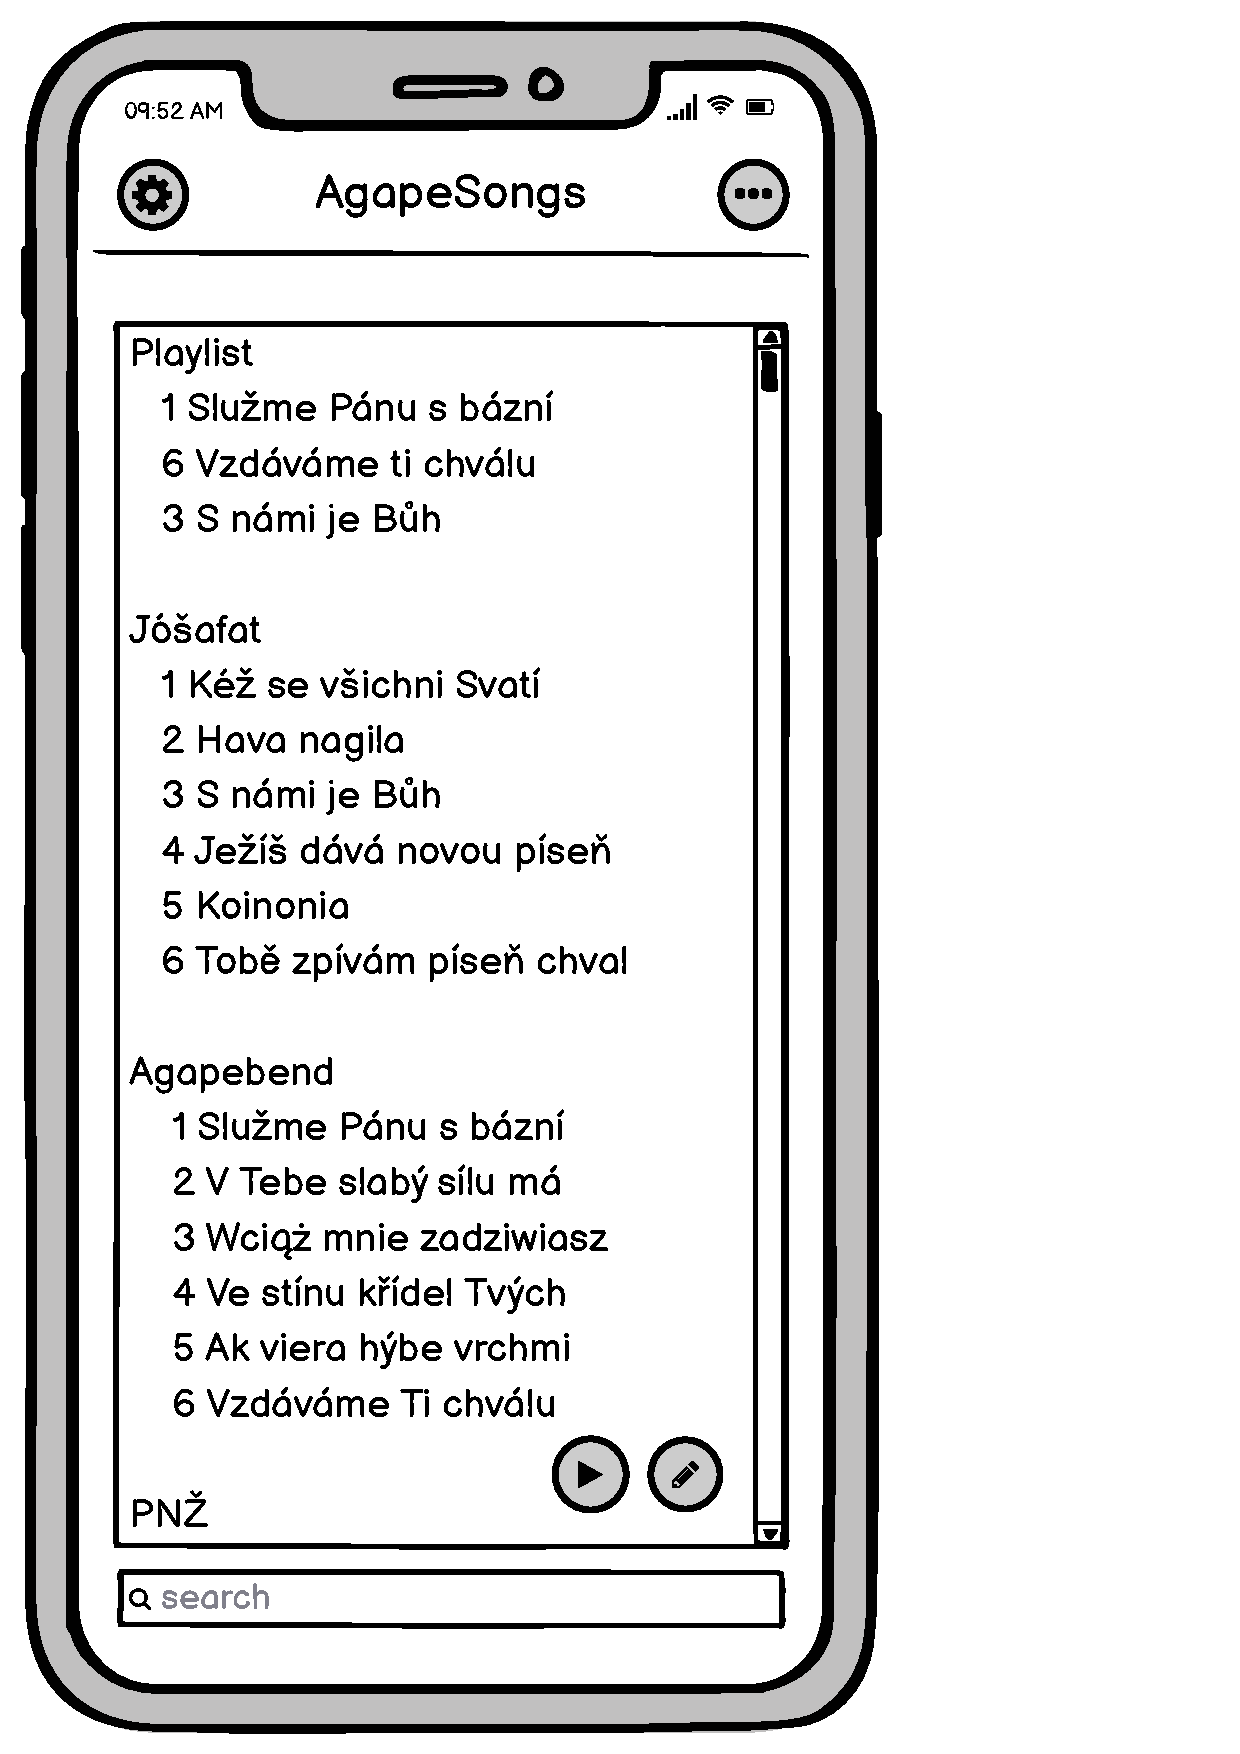
\includegraphics[width=\textwidth/3 - 2pt]{images/3-navrh/3-6-seznam-zpevniku.pdf}
    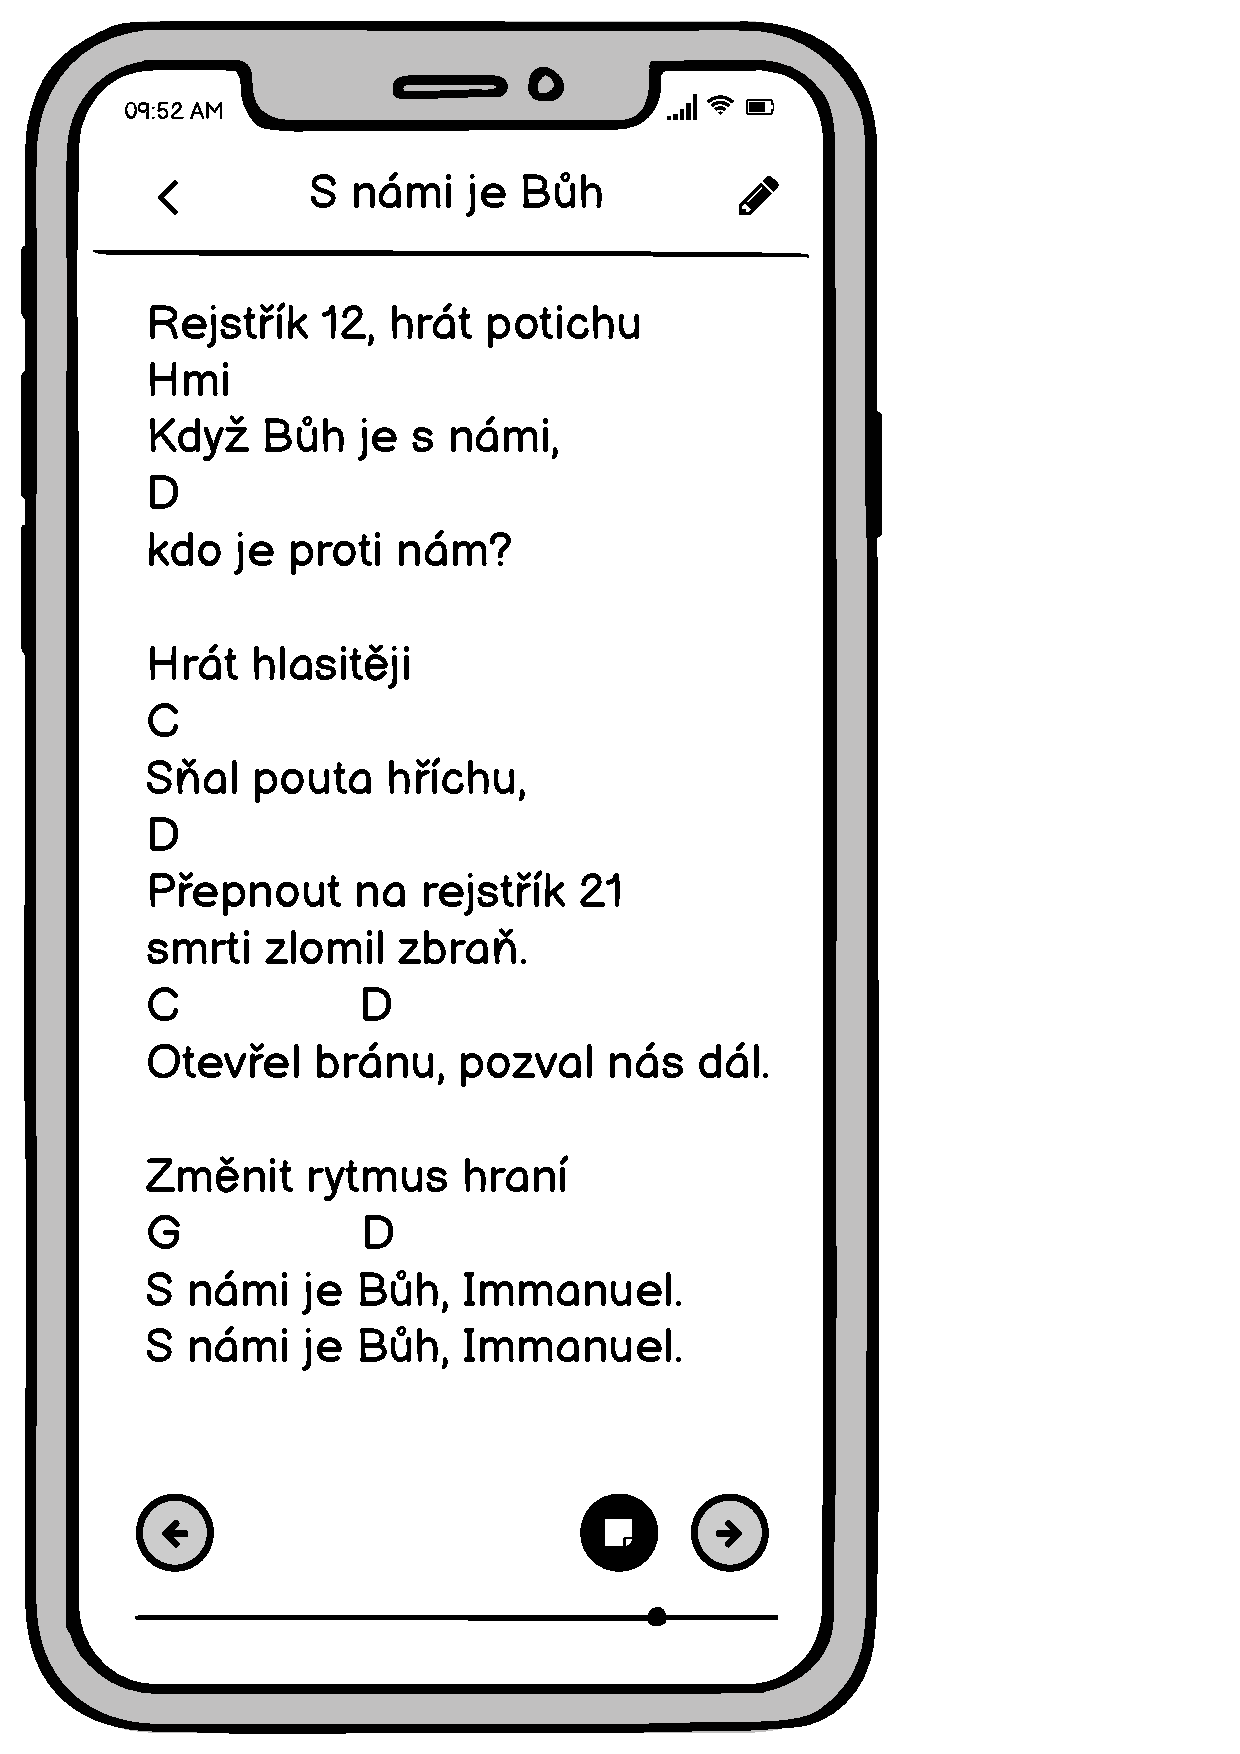
\includegraphics[width=\textwidth/3 - 2pt]{images/3-navrh/3-6-detail-pisne-clen.pdf}
    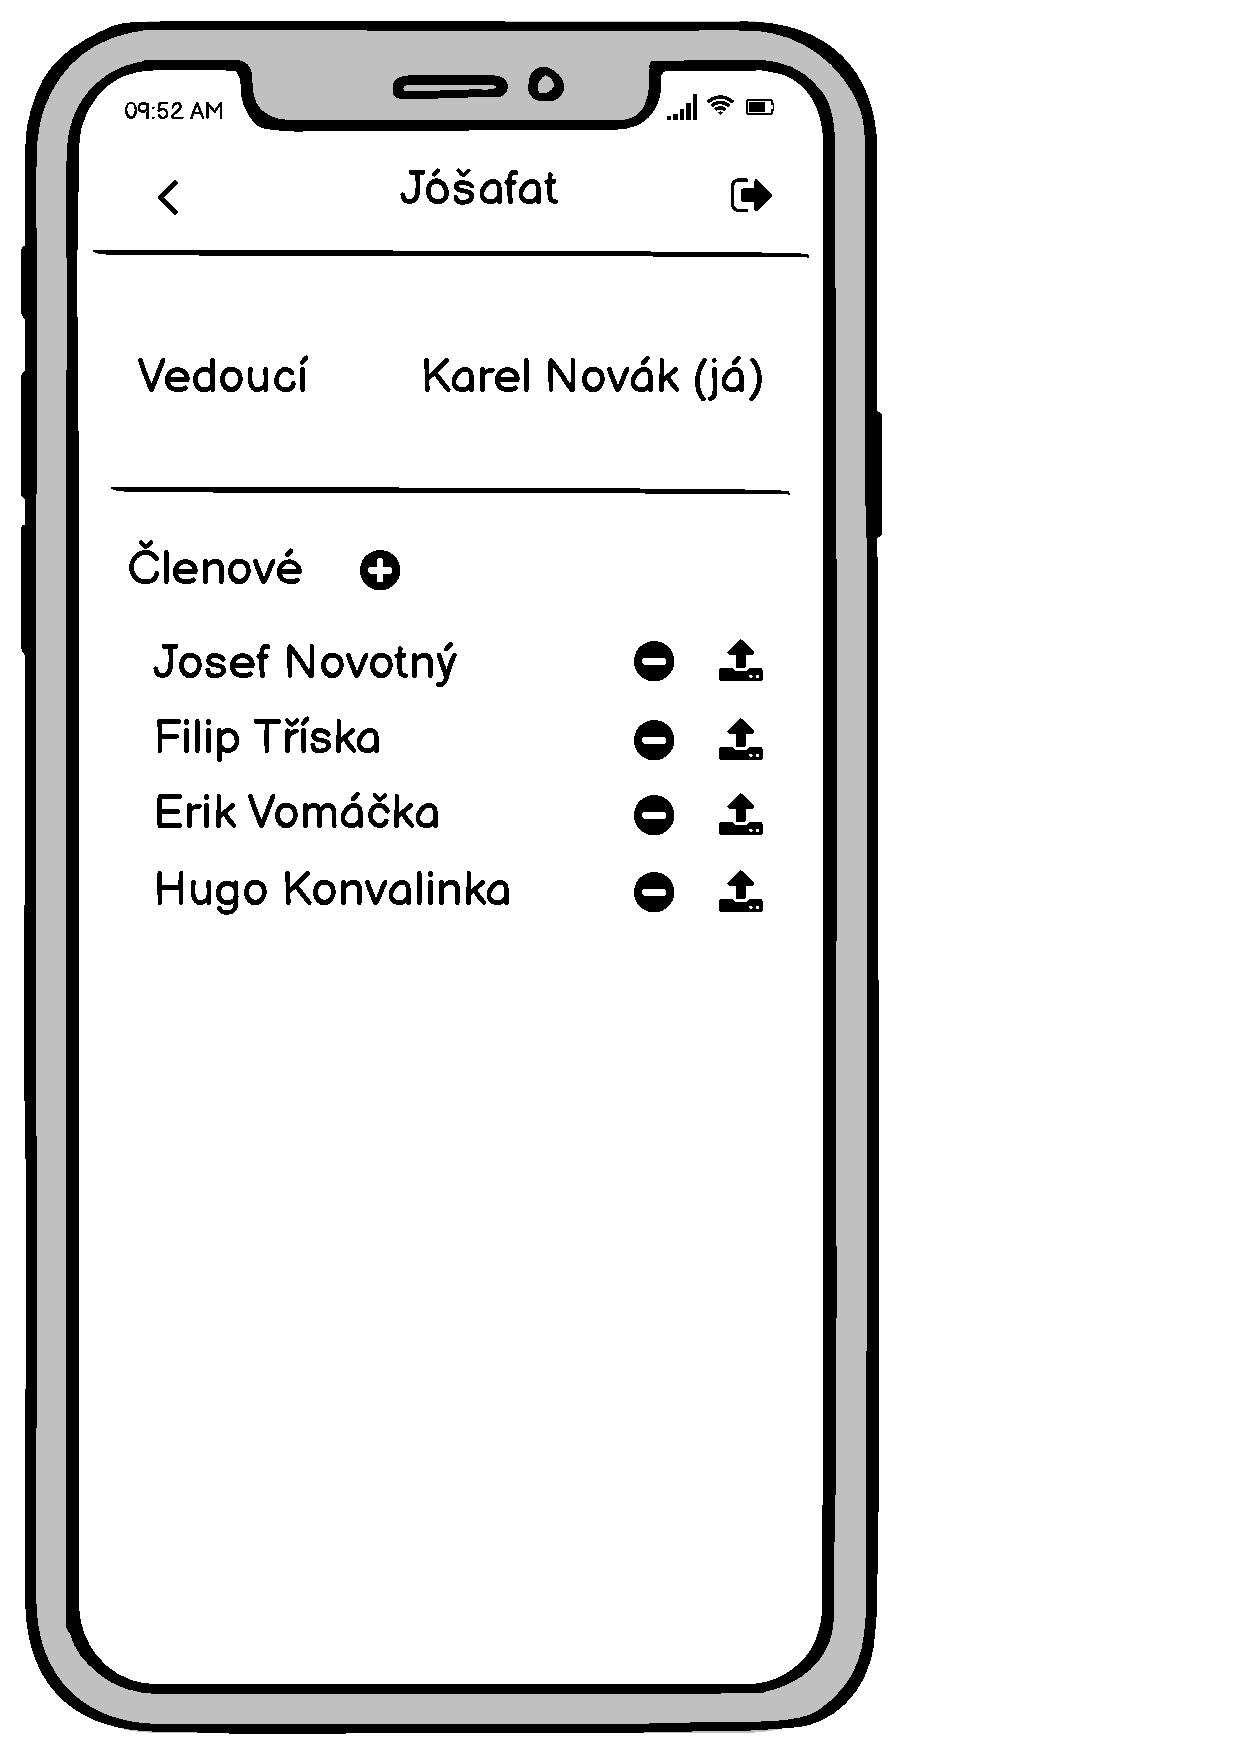
\includegraphics[width=\textwidth/3 - 2pt]{images/3-navrh/3-6-detail-kapely-vedouci.pdf}
    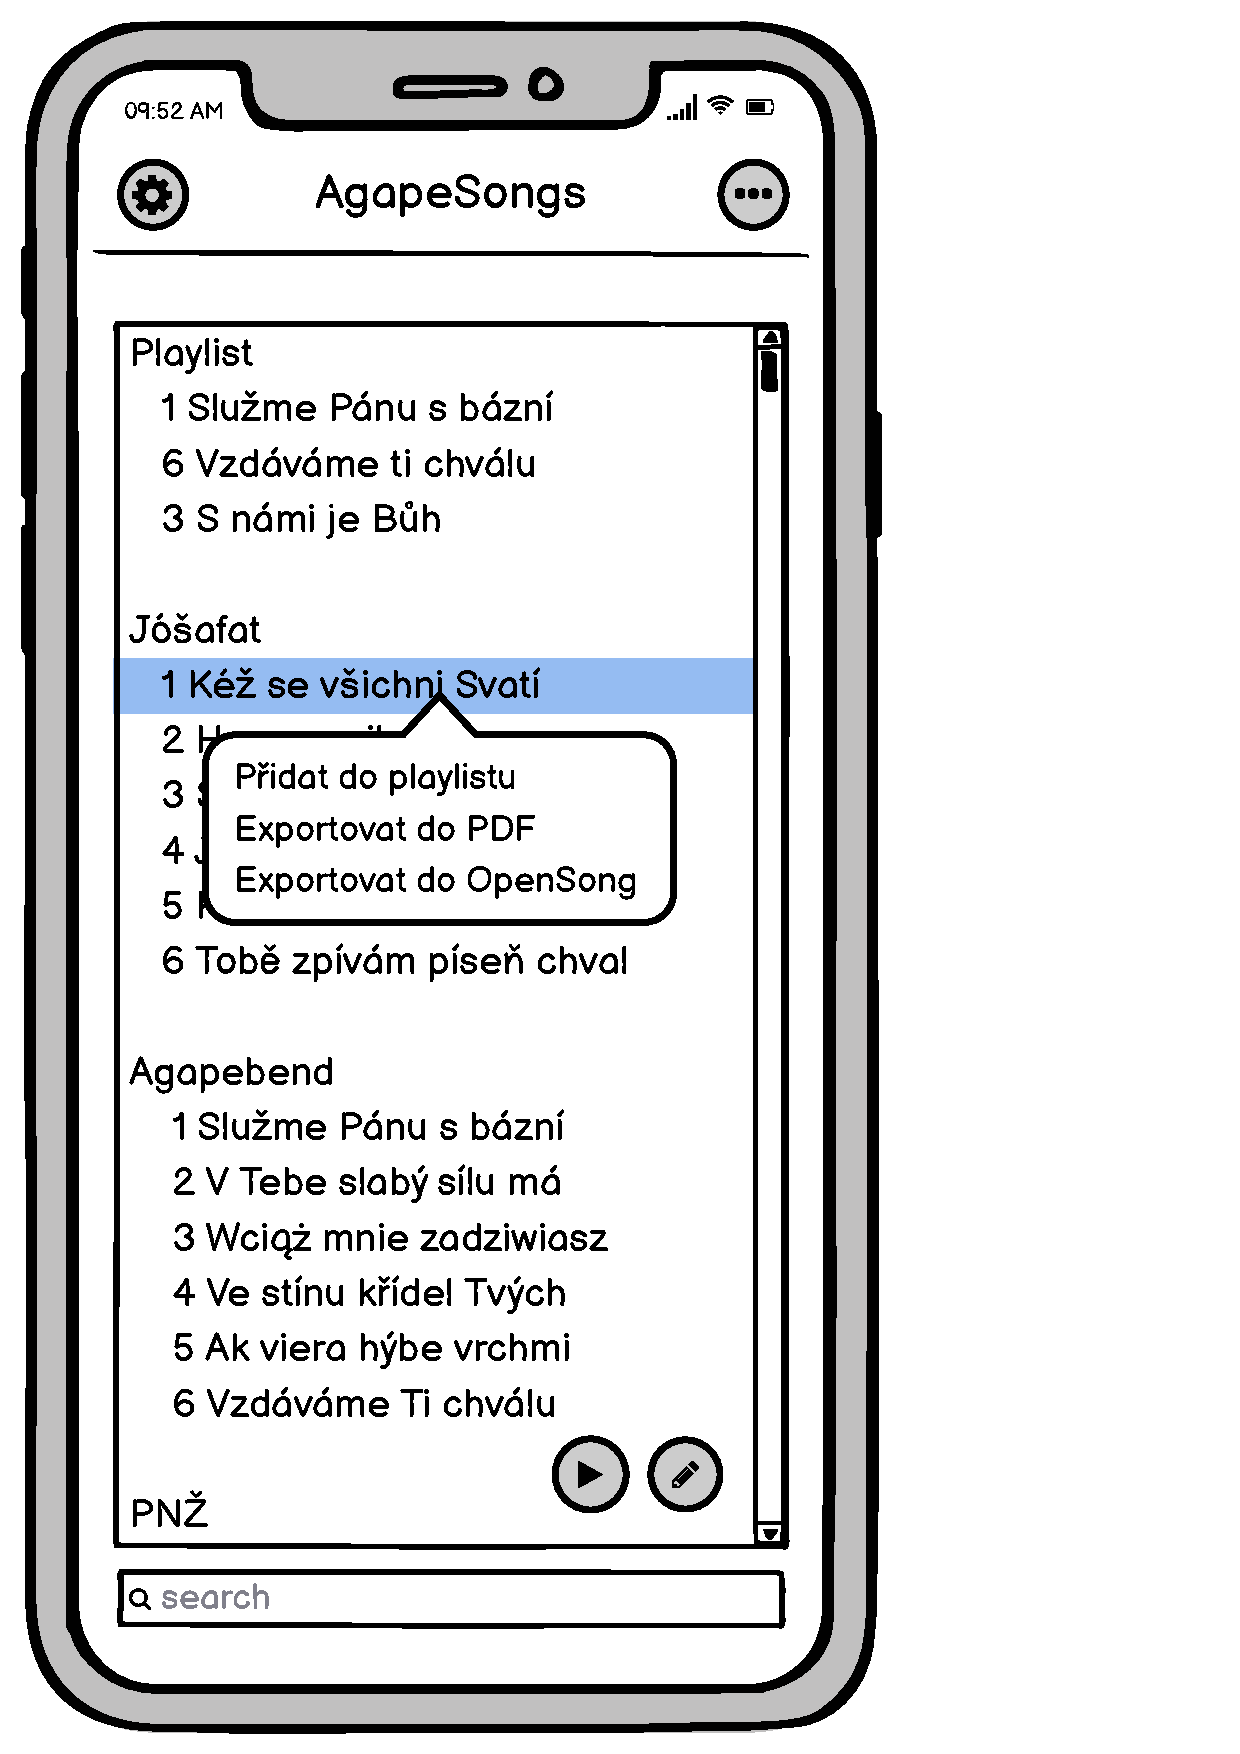
\includegraphics[width=\textwidth/3 - 2pt]{images/3-navrh/3-6-seznam-zpevniku-kontextove-menu.pdf}
    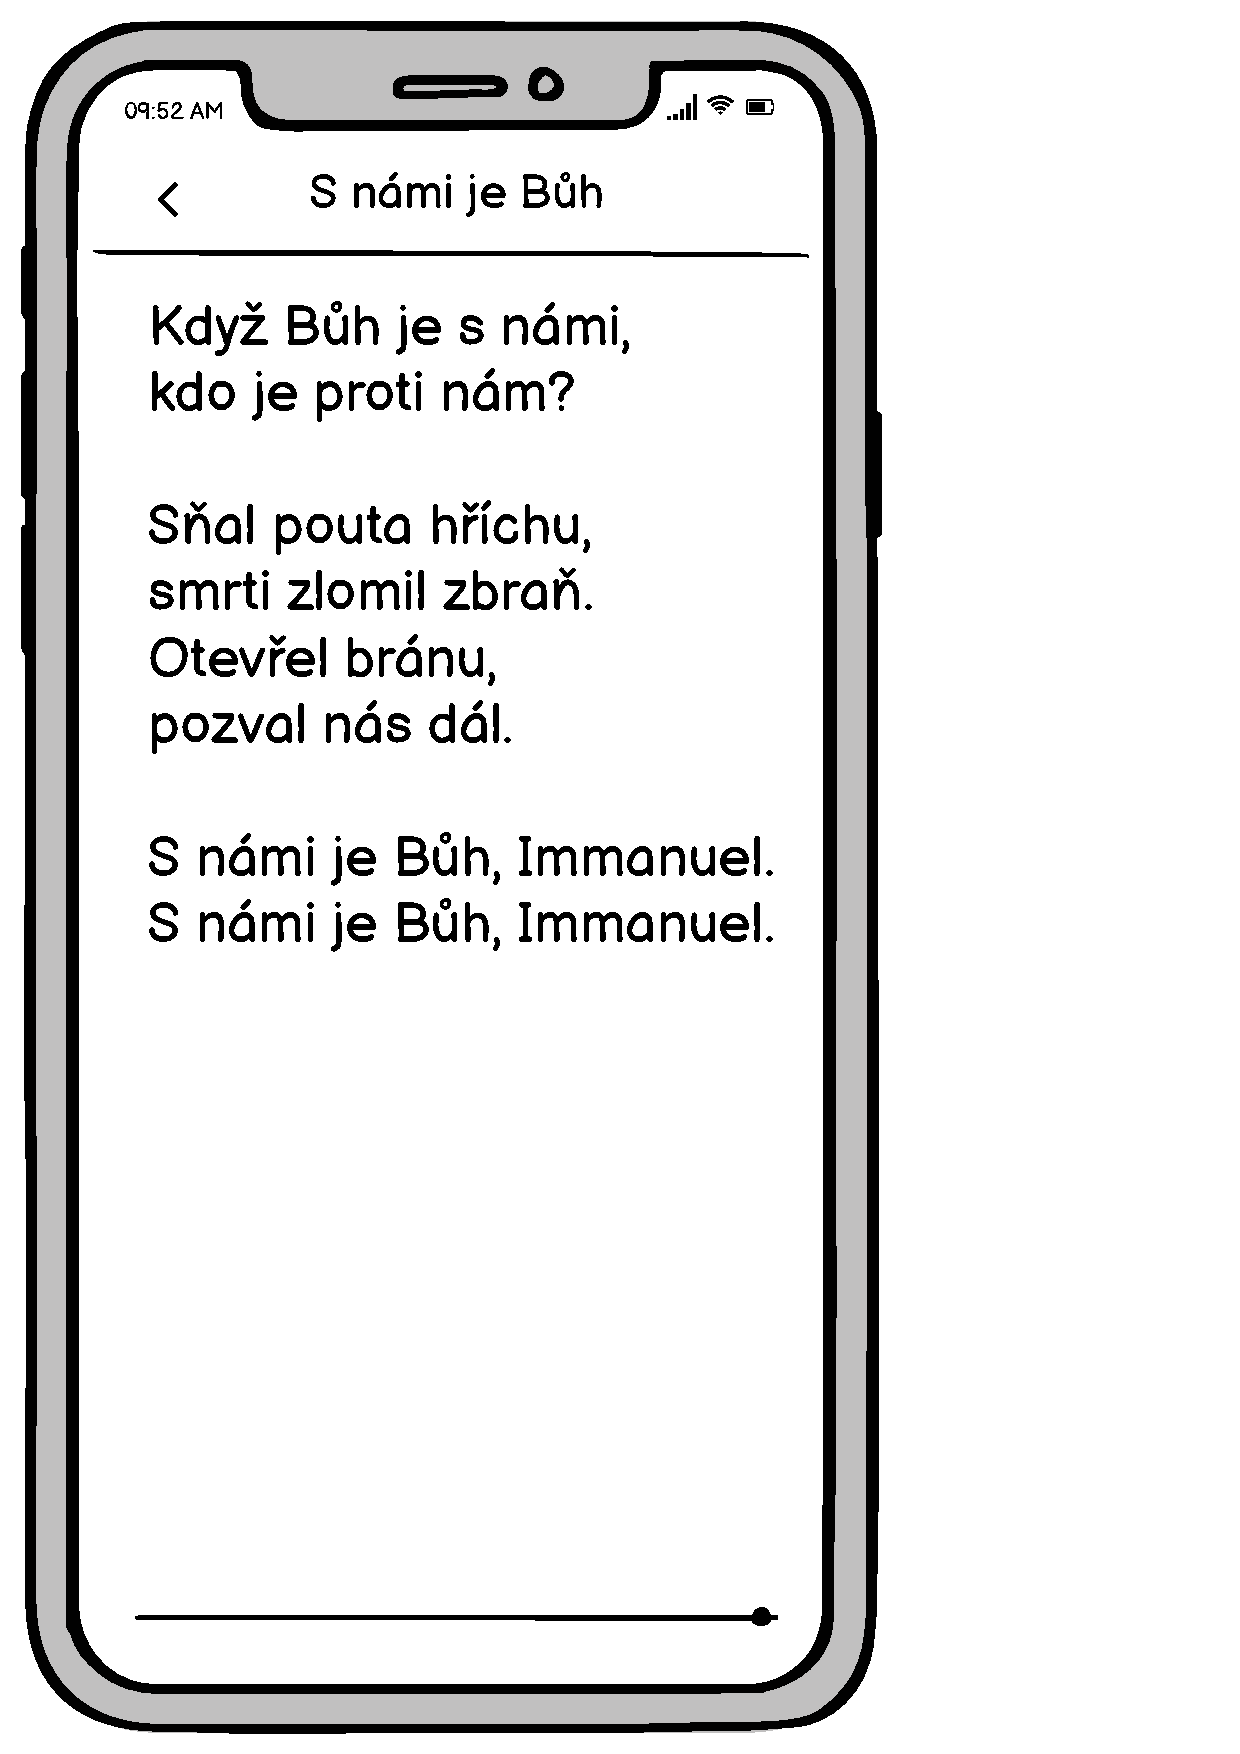
\includegraphics[width=\textwidth/3 - 2pt]{images/3-navrh/3-6-detail-pisne-host.pdf}
    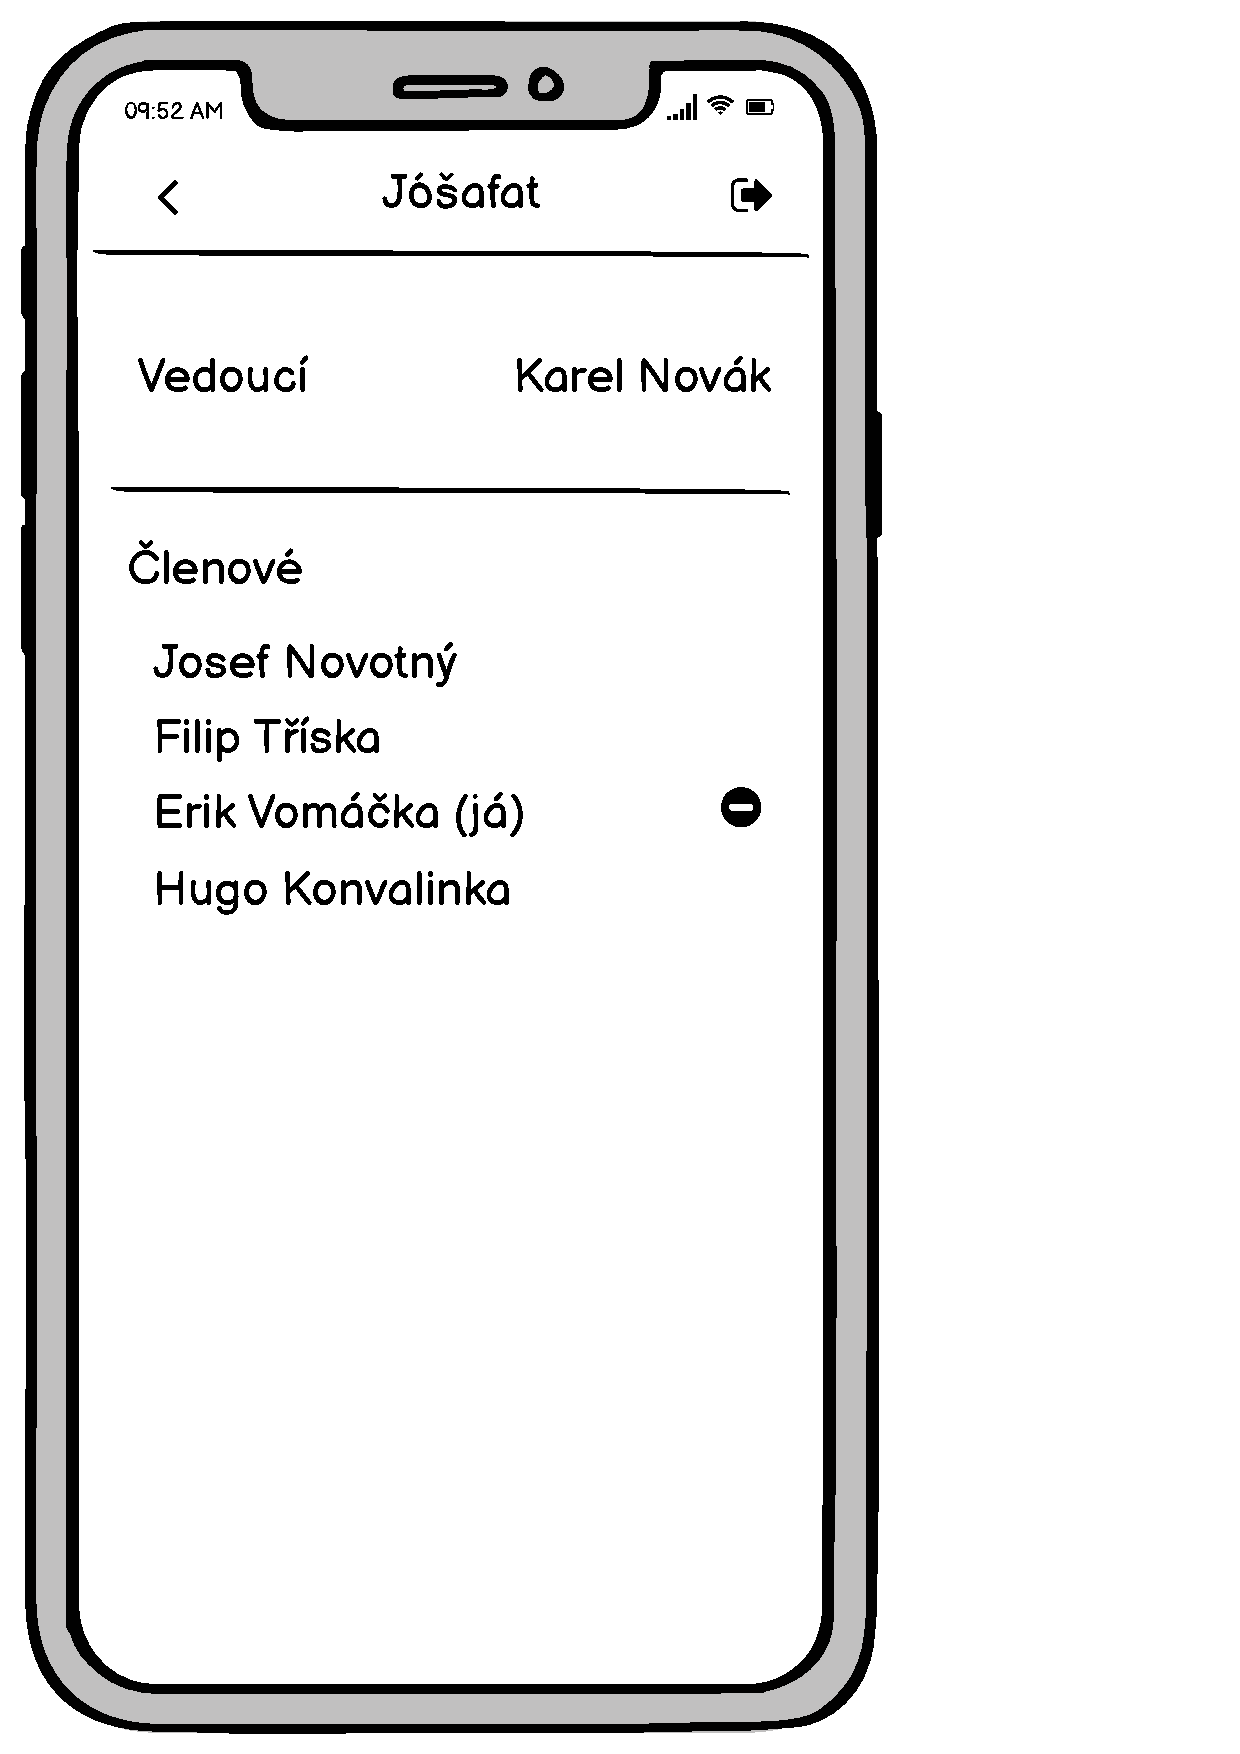
\includegraphics[width=\textwidth/3 - 2pt]{images/3-navrh/3-6-detail-kapely-clen.pdf}
    \caption[Prototyp uživatelského rozhraní -- Seznam písní, Detail písně a Detail kapely]{Prototyp uživatelského rozhraní -- Seznam písní a zpěvníků (dole s kontextovou nabídkou), Detail písně (nahoře pohled hudebníka, dole pohled zpěváka) a Detail kapely (nahoře pohled vedoucího, dole pohled člena kapely)}
\end{figure}

\subsection{Dialogy}

V aplikaci používám tři typy dialogů:

\begin{itemize}
    \item \textbf{Popover} -- dialog, který se zobrazí ve formě bubliny na tlačítku, typicky v navigační liště. V~aplikaci tento dialog používám pro filtr písní, nastavení písně a nastavení aplikace.
    \item \textbf{Sheet} -- dialog, který se zobrazí jako nová obrazovka, který lze zavřít potáhnutím dolů. Tento dialog používám pro přidávání a úpravy písní, zpěvníků a členů kapely.
    \item \textbf{Alert} -- dialog zobrazený na obrazovce se ztmavením předchozí obrazovky se dvěma možnost\-mi -- Ano, Ne. Je vhodný především pro potvrzení, ať už potvrzení odebrání zpěvníku nebo člena kapely, stáhnutí či nahrání playlistu nebo změnu oprávnění člena kapely.
\end{itemize}

\begin{figure}
    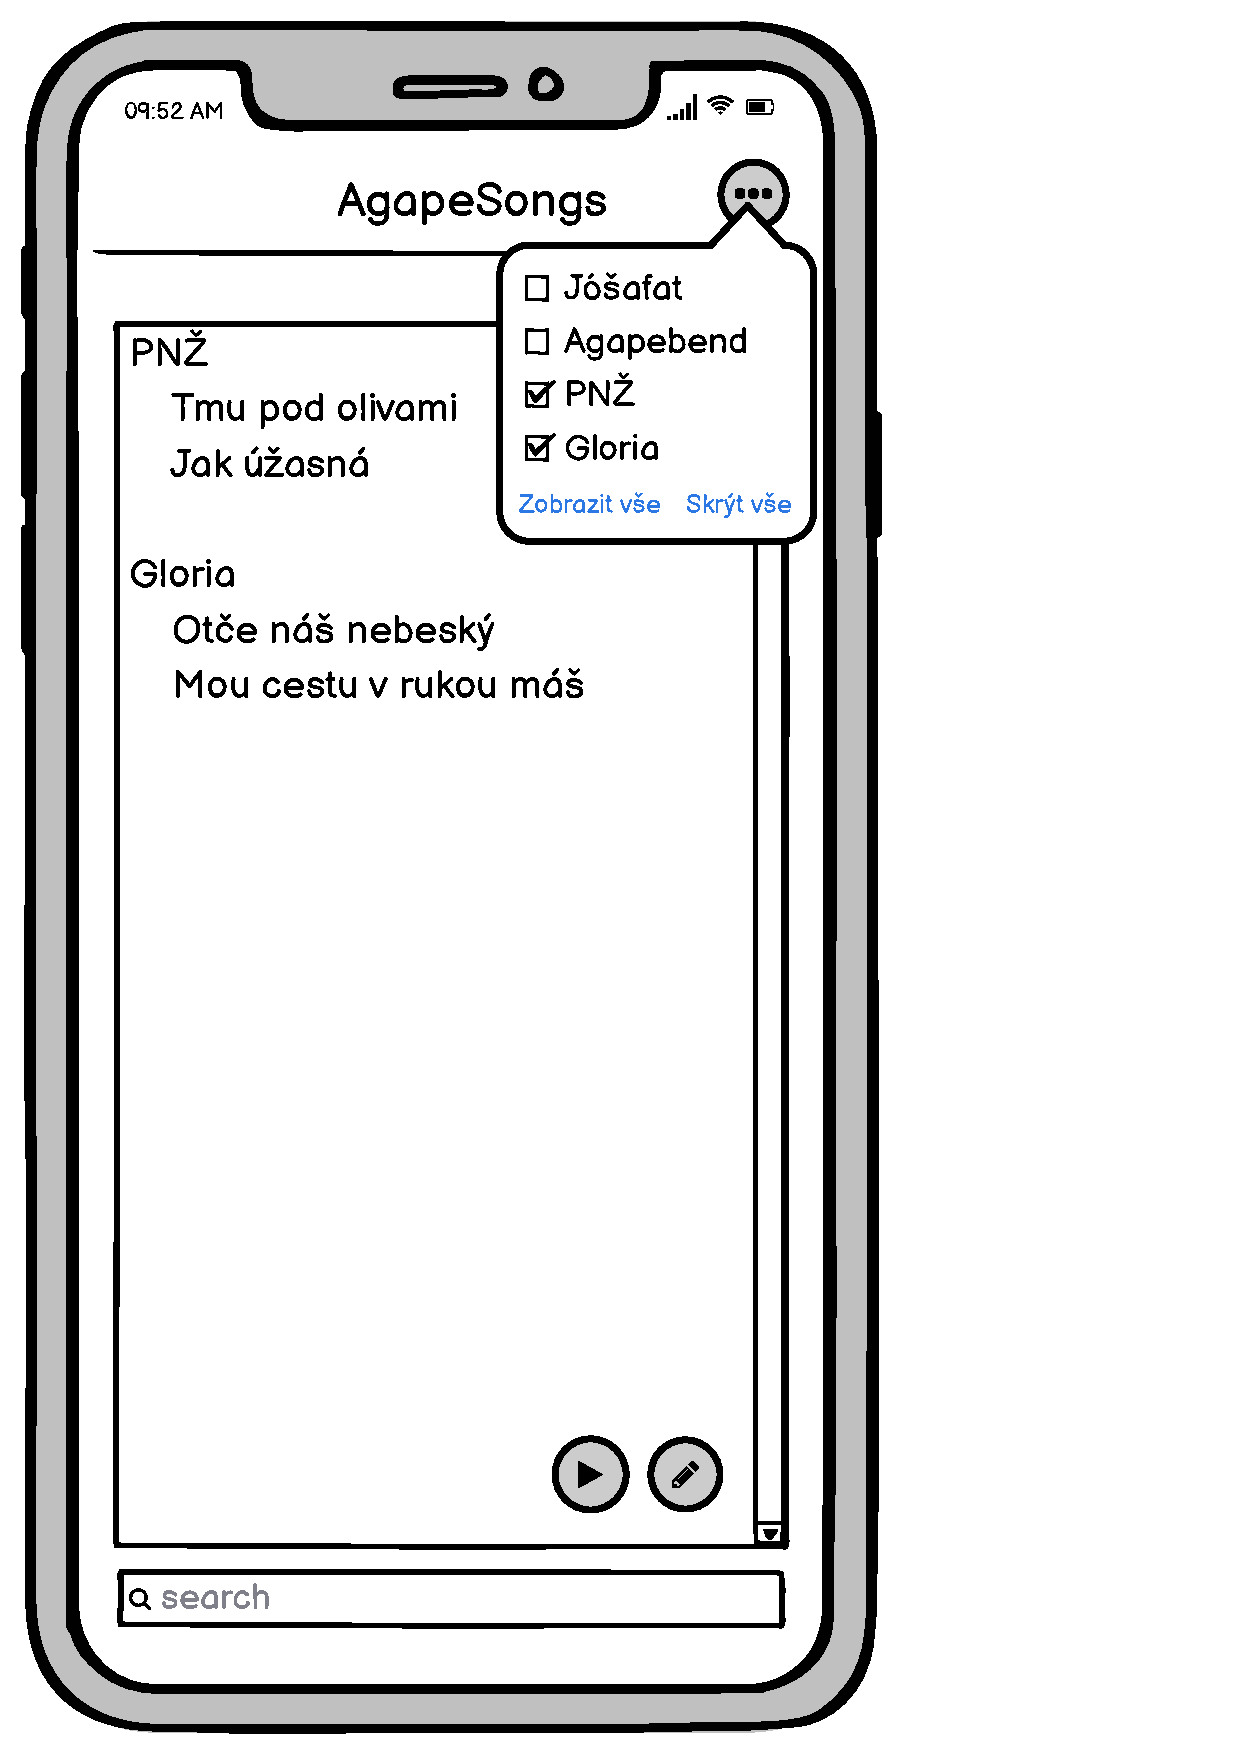
\includegraphics[width=\textwidth/3 - 2pt]{images/3-navrh/3-7-dialog-filtr-zpevniku.pdf}
    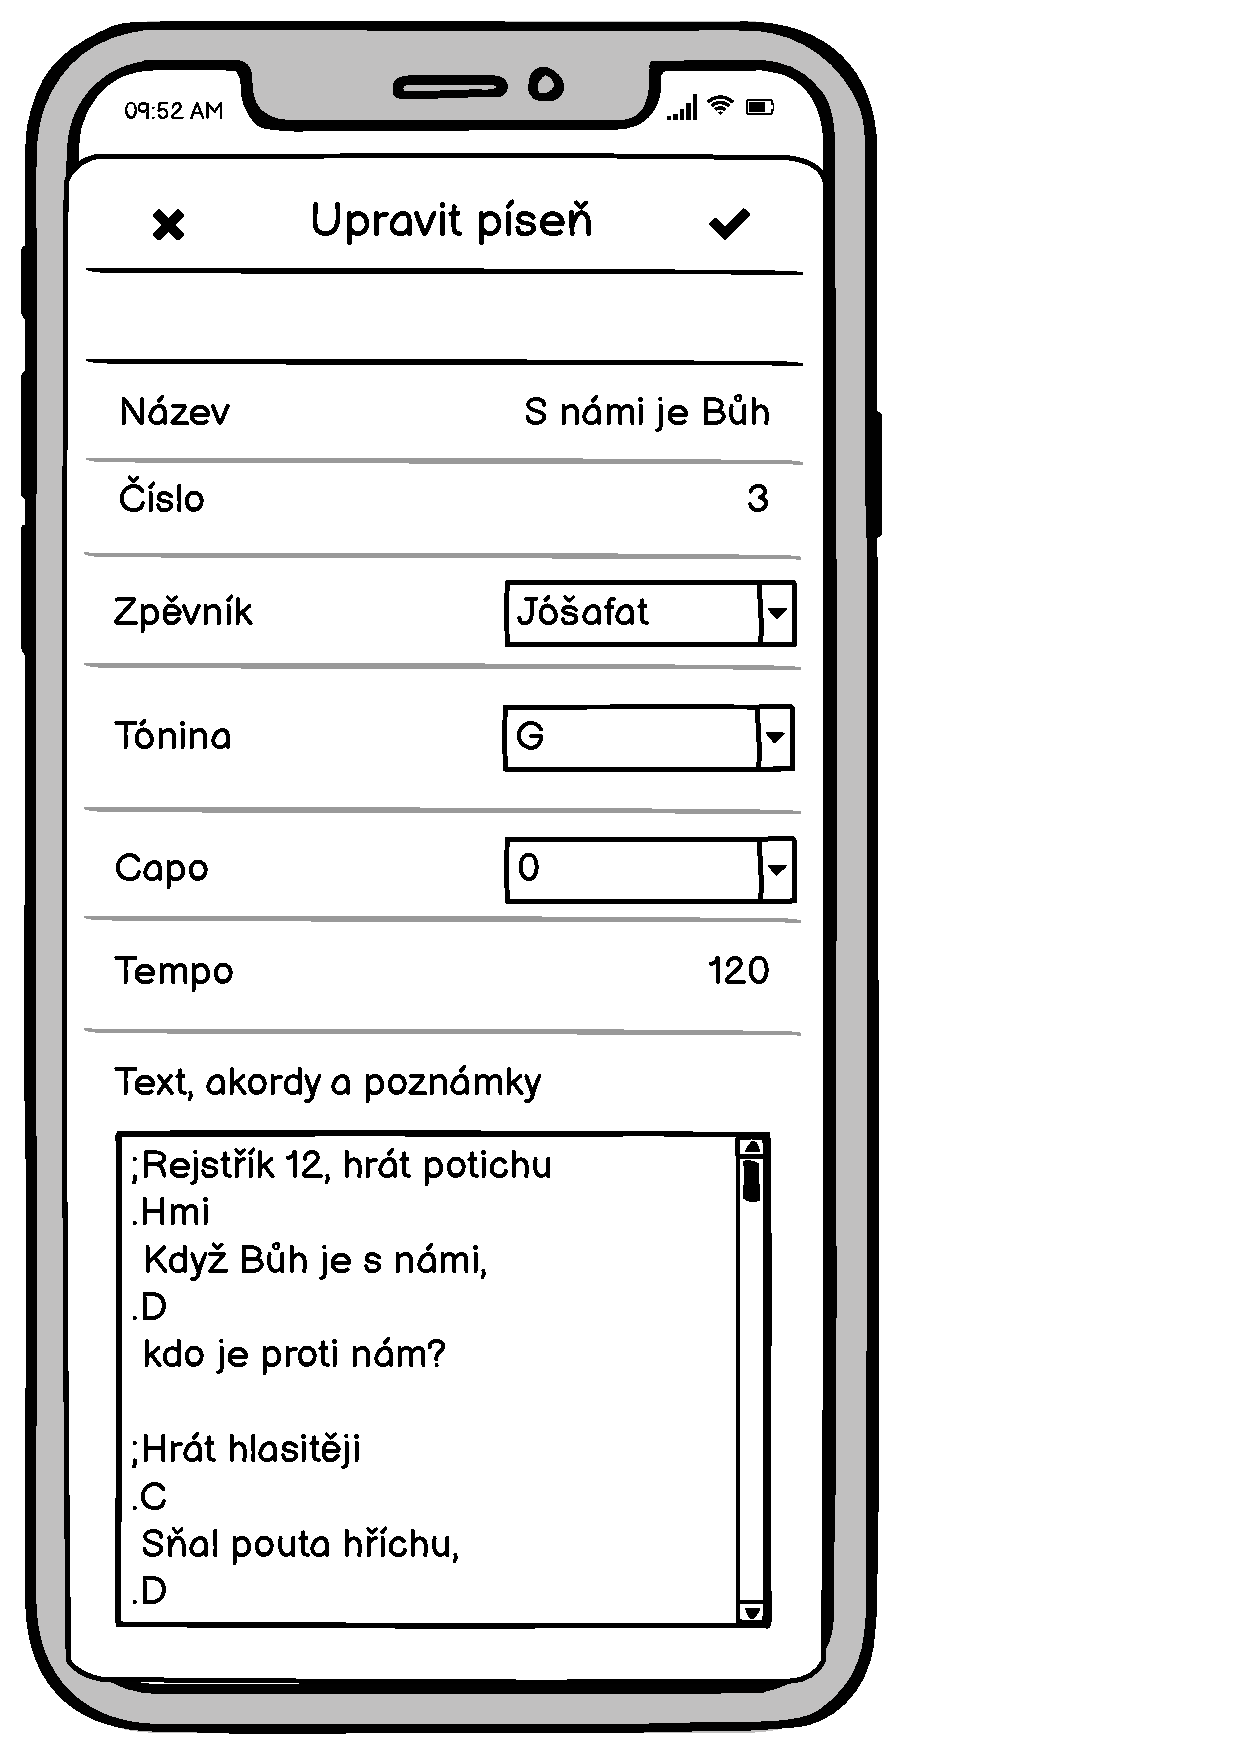
\includegraphics[width=\textwidth/3 - 2pt]{images/3-navrh/3-7-dialog-uprava.pdf}
    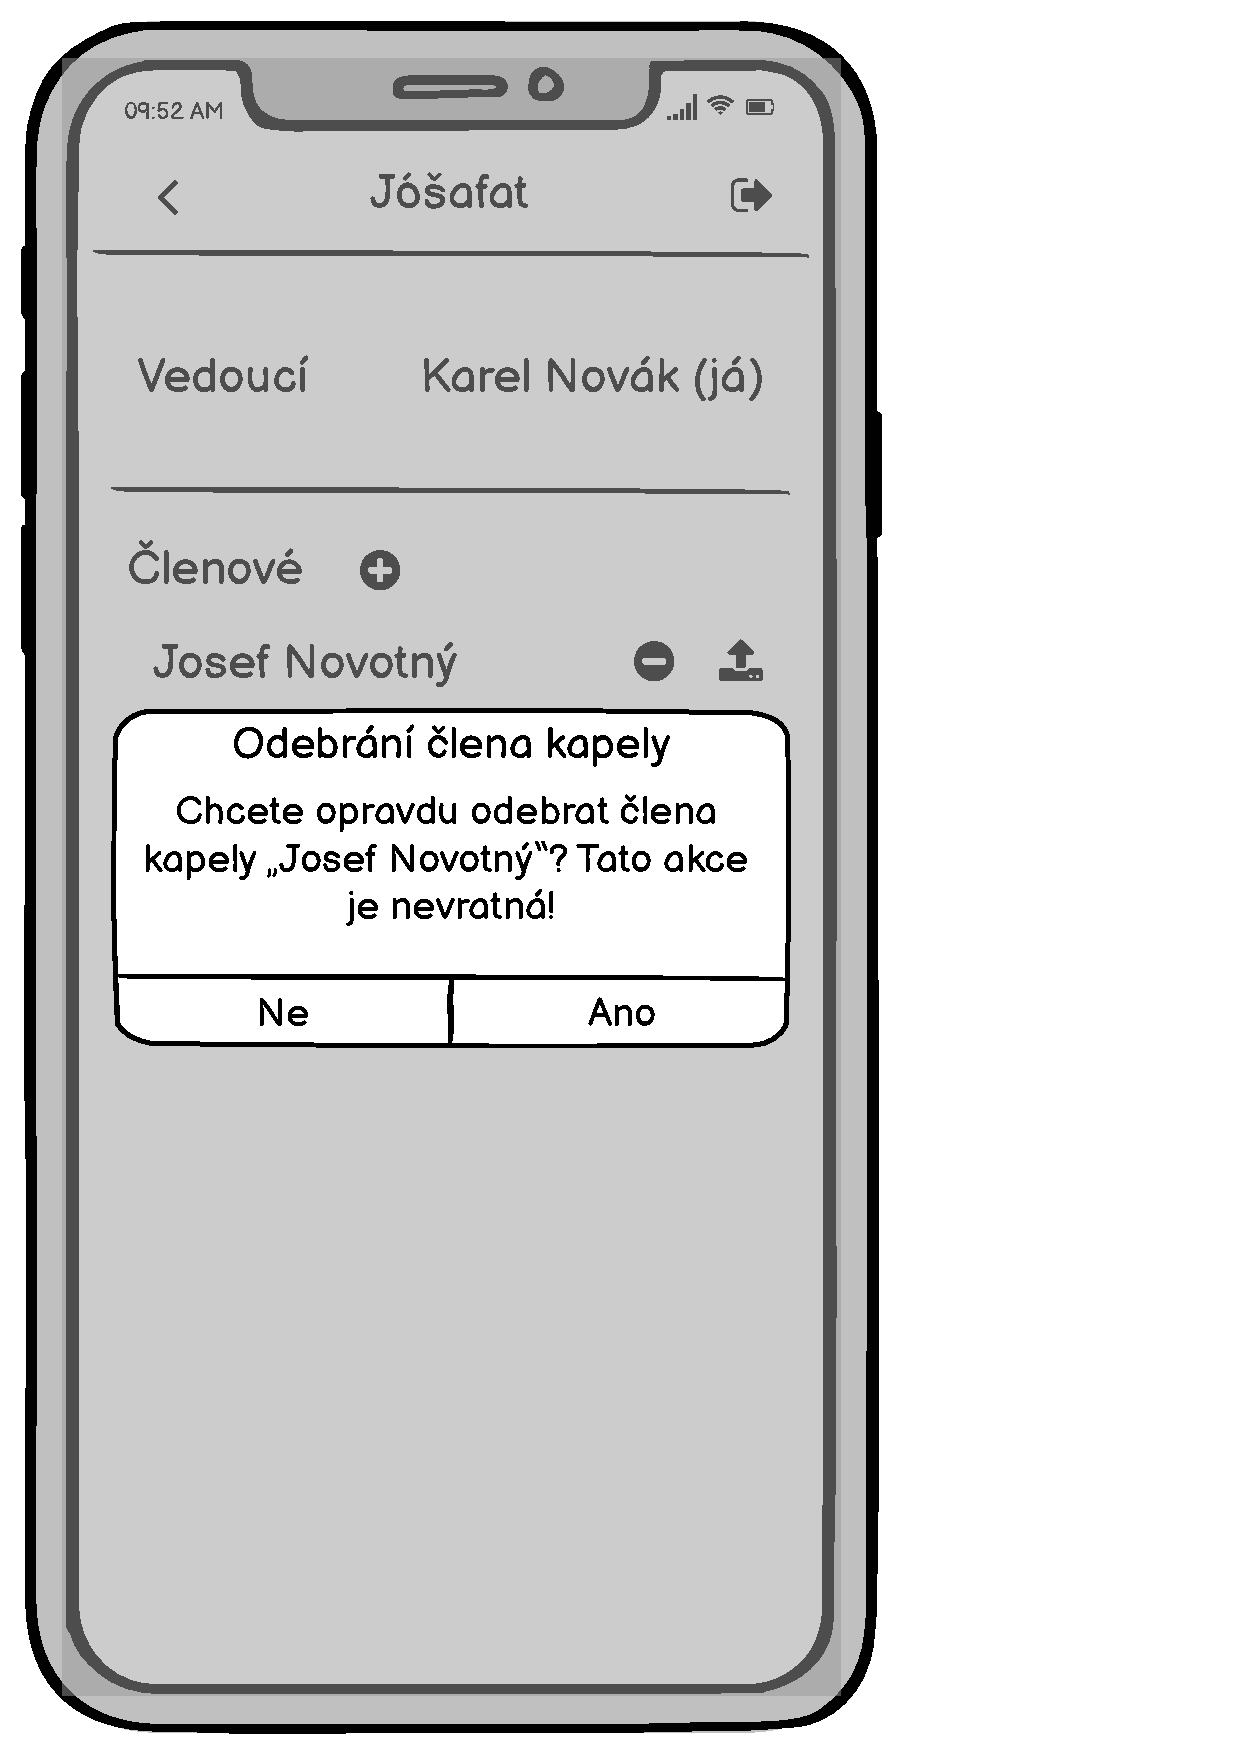
\includegraphics[width=\textwidth/3 - 2pt]{images/3-navrh/3-7-dialog-odebrani.pdf}
    \caption[Prototyp uživatelského rozhraní -- dialogy]{Prototyp uživatelského rozhraní -- Dialog pro filtr zpěvníků (popover), úpravu písně (sheet) a odebrání člena kapely (alert)}
\end{figure}

%---------------------------------------------------------------
\chapter{Implementace serveru}
%---------------------------------------------------------------

\begin{chapterabstract}
    V této kapitole popíšu průběh implementace serveru, jednotlivé třídy a zajímavosti, se kterými jsem se při implementaci setkal.
\end{chapterabstract}

\section{Úvod}

Pro implementaci serveru jsem se rozhodl využít technologii Spring Web \cite{spring-web} v programovacím jazyce Kotlin \cite{kotlin}. Nad touto technologií jsem postavil vlastní nadstavbu, která s pomocí šablon generuje velkou část obecného kódu pro zpřístupnění dat s pomocí REST API. Implementace těchto základních CRUD (z anglického Create = vytvoření, Read = čtení, Update = úprava, Delete = smazání) operací je tak velmi rychlá a spočívá především v definici dat v databázi (datová vrstva, balíček Entity), definici tříd pro přenos dat mezi business a prezentační vrstvou (business vrstva, balíček DTO) a definici oprávnění pro jednotlivé operace (prezentační vrstva, balíček Controller).

\section{Datová vrstva}

Datová vrstva se skládá ze dvou balíčků, Entity a Repository. Tato vrstva je obstarána frameworkem Spring JPA \cite{spring-jpa}. Pro zpřístupnění základních CRUD operací jsem tedy pouze vytvořil rozhraní Repository s danou Entitou jako parametrem šablony, konkrétní implementaci včetně komunikace s databází vygeneroval framework.

\subsection{Entity}

Entity jsou reprezentovány jako datové třídy v Kotlinu. Každá entita reprezentuje jednu tabulku v relační databázi a pomocí anotací u proměnných definuji jednotlivé sloupce těchto tabulek včetně integritních omezení a cizích klíčů (vazeb s ostatními entitami). Entity, se kterými pracuji, jsou uživatel (User), zpěvník (SongBook), píseň (Song), poznámka (SongNote), kapela (Band), role (Role) a členství v kapele (BandMember).

Každá entita obsahuje unikátní identifikátor, který je primárním klíčem v databázi a metody \texttt{canView} (může vidět) a \texttt{canEdit} (může upravit), které určují, zda má daný uživatel přístup k~dané entitě.

\begin{listing}
\begin{minted}[breaklines,breaksymbolleft=]{kotlin}
@Entity
@Table (uniqueConstraints=[UniqueConstraint(columnNames = ["name", "band_id"])])
data class SongBook (
    @Column(nullable = false) val name: String,
    @OneToMany(mappedBy = "songBook")
    val songs: List<Song>,

    @ManyToOne
    @JoinColumn (name = "band_id", nullable = false)
    val band: Band,
    override val id: Int = 0
) : IEntity(id) {
    override fun canEdit (user: User)
        = user.bands.any { it.role.level == RoleLevel.LEADER && it.band.id == band.id }
    override fun canView (user: User?)
        = user?.bands?.any { it.band.id == band.id } ?: false
}
\end{minted}
\caption[Ukázka třídy pro zpěvník]{Ukázka třídy pro zpěvník (SongBook). V definici lze vidět integritní omezení -- unikátní klíč na sloupcích jméno a identifikátor kapely, textový sloupec pro jméno, definici 1:N vazby s entitou píseň (Song), M:1 vazby s entitou kapela (Band), kde bude spojení provedeno přes sloupec band\_id a metody \texttt{canEdit} a \texttt{canView}, které umožní uživateli zpěvník upravit/zobrazit, pokud je vedoucím/členem kapely, v níž je aktuální zpěvník}
\end{listing}

\subsection{Repository}

Repository jsou ve Spring JPA definovány pouze jako rozhraní. Metody pro základní CRUD operace jsou vygenerovány frameworkem a není je třeba zvlášť definovat. Pro hledání podle jiných kritérií než je identifikátor entity -- například hledání zpěvníků podle kapel, písní podle zpěvníků nebo poznámek podle uživatele je nezbytné definovat novou metodu (implementaci vygeneruje JPA) s pomocí anotace \texttt{@Query} a dotazu napsaného v dotazovacím jazyce JPQL (Jakarta Persistence Query Language) \cite{jpql}.

\begin{listing}[H]
\begin{minted}[breaklines,breaksymbolleft=]{kotlin}
@Repository
interface SongBookRepository : IRepository<SongBook> {
    @Query("SELECT sb FROM SongBook sb WHERE sb.band IN :bands")
    fun findByBands(bands: List<Band>) : List<SongBook>
}
\end{minted}
\caption[Ukázka třídy Repository pro zpěvník]{Ukázka třídy SongBookRepository s metodou pro hledání zpěvníků podle kapel}
\end{listing}

\section{Business vrstva}

Business vrstva se skládá ze dvou balíčků, Service a DTO. Cílem business vrstvy je zprostředkovat data z datové vrstvy a odpovědět s jejich pomocí na dotazy z prezentační vrstvy. Tato vrstva je částečně obstarána mou nadstavbou, pro zpřístupnění základních CRUD operací tak stačí vytvořit třídu Service, která dědí z abstraktní šablony \texttt{IServiceImpl} s danou entitou a DTO jako parametry této šablony.

\subsection{DTO}

DTO (z anglického data transfer object) jsou speciální datové třídy, které slouží ke komunikaci mezi business a prezentační vrstvou. Existují DTO tří typů -- DTO ke čtení (\texttt{IReadDTO}), k~úpravě (\texttt{IUpdateDTO}) a k vytvoření (\texttt{ICreateDTO}). Každé \texttt{IReadDTO} musí obsahovat identifikátor entity a slouží k zprostředkování dat \textbf{z databáze} směrem k prezentační vrstvě. \texttt{ICreateDTO} a \texttt{IUpdateDTO} slouží k vytváření a úpravě entity a zprostředkovávají data z prezentační vrstvy směrem \textbf{do~databáze}. Rozdíl mezi \texttt{ICreateDTO} a \texttt{IUpdateDTO} je pak ten, že \texttt{IUpdateDTO} má nepovinné parametry -- parametry, které budou vynechány, nebudou aktualizovány.

\begin{listing}[H]
\begin{minted}[breaklines,breaksymbolleft=]{kotlin}
data class SongBookReadDTO (override val id: Int, val name: String, val band: BandReadDTO, val songs: List<SongReadDTO>) : IReadDTO
data class SongBookUpdateDTO (val name: String?, val bandId: Int?) : IUpdateDTO
data class SongBookCreateDTO (val name: String, val bandId: Int) : ICreateDTO
\end{minted}
\caption[Ukázka DTO tříd pro zpěvník]{Ukázka souboru s DTO třídami pro zpěvník (SongBookDTO). Při čtení se zde vrací jméno zpěvníku, DTO popisující kapelu a seznam písní ve zpěvníku. Při vytváření/úpravě zpěvníku se používá jméno a identifikátor kapely, zpěvník se vytvoří bez písní}
\end{listing}

\subsection{Service}

Každá Service je implementací obecného rozhraní \texttt{IService}, které obsahuje základní CRUD metody. Jejich implementaci spolu s autorizací pak zajišťuje abstraktní šablona \texttt{IServiceImpl}. Má nadstavba umožňuje také vytvoření Service bez CRUD operací, ta pak dědí přímo z abstraktní třídy \texttt{IServiceBase}, která obsahuje metodu pro autorizaci uživatele pomocí \texttt{UserReadDTO} (získané při autentizaci) a metodu \texttt{tryCatch}, která zajišťuje správné zpracování výjimek.

Při práci s jednotlivými Repository je při chybě (neexistující entita, porušené integritní omezení) vyhozena výjimka z JPA. Tuto výjimku ale Spring Web neumí zpracovat a pokud by nebyla odchycena, server by v takovém případě místo chybového kódu 404 (nenalezeno) nebo 400 (špatný požadavek) vrátil kód 500 (chyba serveru). Veškeré operace tedy musí být obaleny v bloku \texttt{tryCatch}, který tyto výjimky odchytí a nahradí správnou výjimkou \texttt{ResponseStatusException} s příslušným HTTP kódem, kterou již Spring Web dokáže zpracovat.

\begin{listing}[H]
\begin{minted}[breaklines,breaksymbolleft=]{kotlin}
protected fun <X> tryCatch (block: IRepository<T>.() -> X) = 
    try { repository.block() }
    catch (_: JpaObjectRetrievalFailureException) { throw ResponseStatusException(HttpStatus.NOT_FOUND) }
    catch (_: EmptyResultDataAccessException)     { throw ResponseStatusException(HttpStatus.NOT_FOUND) }
    catch (e: ResponseStatusException)            { throw e } // rethrow ResponseStatusException
    catch (_: Exception)                          { throw ResponseStatusException(HttpStatus.BAD_REQUEST) }
\end{minted}
\caption[Pomocná metoda pro zaobalení výjimek ze Spring JPA]{Pomocná metoda, která zaobalí předaný blok, odchytí výjimky ze Spring JPA a převede je na výjimku \texttt{ResponseStatusException}. V případě úspěchu vrátí návratovou hodnotu předaného bloku}
\end{listing}

Tyto třídy před zpřístupněním entity ke čtení/úpravě zkontrolují, zda má aktuální uživatel (pokud je přihlášen) právo k této entitě přistupovat. Pokud není přihlášen žádný uživatel, vyhodí výjimku \texttt{ResponseStatusException} s kódem 401 (neautentifikován), pokud nemá dostatečná oprávnění, výjimka je vyhozena s kódem 403 (neautorizován).

Jelikož třídy z balíčku Service pracují s DTO a entitami, musí každá třída implementující rozhraní \texttt{IService} obsahovat metodu \texttt{Entity.toDTO()} pro převod z entity do příslušného \texttt{IReadDTO}, \texttt{ICreateDTO.toEntity()} pro převod z \texttt{ICreateDTO} do příslušné entity
a také \texttt{Entity.merge(} \texttt{IUpdateDTO)}, která na předané entitě změní všechny parametry, které nejsou \texttt{null} v \texttt{IUpdateDTO}. Kromě toho tyto třídy obsahují i pomocné metody pro převod dalších DTO -- například v případě Service pro zpěvník je zde obsažena i metoda pro převod kapely. Při takovém převodu ale již nejsou převáděny zpěvníky, aby nedošlo k zacyklení, a seznam zpěvníků v kapele je tak prázdný.

\begin{listing}
\begin{minted}[breaklines,breaksymbolleft=]{kotlin}
// === INTERFACE METHOD IMPLEMENTATION ===
override fun SongBook.toDTO () : SongBookReadDTO = SongBookReadDTO(id, name, band.toDTO(), songs.map { it.toDTO() })
override fun SongBookCreateDTO.toEntity () = SongBook(name, emptyList(), bandRepository.getById(bandId))
override fun SongBook.merge (dto: SongBookUpdateDTO) = copy(
    name = dto.name ?: name,
    band = dto.bandId?.let { bandRepository.getById(it) } ?: band
)

// === HELPER METHODS ===
private fun Song.toDTO () = SongReadDTO(id, songBook.copy(songs = emptyList()).toDTO(), name, songService.convertSongText(text), SongKey.valueOf(key), bpm, capo, lastEdit, displayId, null)
private fun SongNote.toDTO () = SongNoteReadDTO(id, notes, capo, lastEdit)
private fun Band.toDTO () = BandReadDTO(id, name, members.map { it.toDTO() })

private fun BandMember.toDTO () = BandMemberReadDTO(id, BandReadDTO(band.id, band.name, emptyList()), user.toDTO(), role.toDTO())
private fun User.toDTO () = UserReadDTO(id, email, name, emptyList())
private fun Role.toDTO () = RoleReadDTO(id, level.name)
\end{minted}
\caption[Ukázka třídy Service pro zpěvník]{Ukázka metod pro převod DTO zpěvníku a pomocné metody pro převod DTO písně, poznámky, kapely, členství v kapele, uživatele a role}
\end{listing}

\section{Prezentační vrstva}

Prezentační vrstva je tvořena jediným balíčkem Controller. Ten obsahuje obecnou abstraktní šablonu \texttt{IController}, která definuje rozhraní metod pro základní CRUD operace. Konkrétní implementaci těchto metod včetně autorizace pak zajišťuje abstraktní třída \texttt{IControllerAuth}. Každý Controller pak dědí z této abstraktní třídy a pomocí anotace \texttt{@VisibilitySettings} definuje viditelnost jednotlivých metod.

Jednotlivé metody v Controlleru jsou namapovány na odpovídající HTTP metody a adresy zdrojů pomocí anotací \texttt{@GetMapping}, \texttt{@PostMapping}, \texttt{@PutMapping} a \texttt{@DeleteMapping}. Hlavičky těchto metod pak můžou obsahovat anotace \texttt{@PathVariable} pro získání proměnné z URL, \texttt{@RequestBody}, která načte daný parametr z těla HTTP požadavku a \texttt{@ResponseStatus}, která určuje základní HTTP návratový kód v případě úspěchu. Také zde lze použít jako parametr třídu \texttt{HttpServletRequest}, která reprezentuje celý HTTP požadavek.

\texttt{IControllerAuth} obsahuje speciální metodu \texttt{authenticate}, která přijímá HTTP požadavek, nastavení viditelnosti a akci k provedení. Tato akce obsahuje parametr \texttt{UserReadDTO}, do kterého je předán přihlášený uživatel. Tuto metodu pak využívají jednotlivé Controllery pro autorizaci a autentifikaci.

\begin{listing}[H]
\begin{minted}[breaklines,breaksymbolleft=]{kotlin}
// IController.kt
protected fun <A> authenticate (request: HttpServletRequest, settings: VisibilitySettings, action: (UserReadDTO?) -> A) : A {
    val loginSecret = request.getHeader("LOGIN_SECRET") ?: ""
    val dto = userService.getByLoginSecret(loginSecret)
    
    when (settings) {
        VisibilitySettings.ALL    -> {}
        VisibilitySettings.LOGGED -> {
            if (dto == null) 
                throw ResponseStatusException(HttpStatus.UNAUTHORIZED)
        }
        VisibilitySettings.NONE   -> {
            throw ResponseStatusException(HttpStatus.METHOD_NOT_ALLOWED)
        }
    }
    
    return action(dto) // Perform requested action with logged user
}

// SongNoteController.kt
@PutMapping
fun putSongNote(@PathVariable id: Int, @PathVariable songId: Int, 
    @RequestBody dto: SongNoteUpdateDTO, request: HttpServletRequest)
    = authenticate(request, VisibilitySettings.LOGGED) {
        user -> service.putSongNote(id, songId, dto, user)
    }
\end{minted}
\caption[Ukázka autentifikace na serveru]{Ukázka metody \texttt{authenticate} ve třídě \texttt{IController} a její využití pro autentifikaci při požadavku na uložení soukromé poznámky k písni ve třídě \texttt{SongNoteController}}
\end{listing}

\section{Dependency Injection}

Dependency Injection je způsob, kterým jsou v aplikaci předávány závislosti do jednotlivých tříd. Framework Spring Web automaticky zajišťuje dependency injection tříd, jako je Repository (\texttt{@Repository}), Service (\texttt{@Service}), Controller (\texttt{@RestController}) a také interních tříd, jako je třída pro HTTP požadavek (\texttt{HttpServletRequest}) v balíčku Controller nebo třída \texttt{Environment} obsahující proměnné z konfiguračního souboru \texttt{application.properties}.

\begin{listing}[H]
\begin{minted}[breaklines,breaksymbolleft=]{kotlin}
@Service
class AuthService(override val repository: UserRepository, private val bandRepository: BandRepository, private val bandMemberRepository: BandMemberRepository, private val roleRepository: RoleRepository, private val songBookRepository: SongBookRepository, private val songRepository: SongRepository, private val networkService: NetworkService, environment: Environment)
\end{minted}
\caption[Ukázka hlavičky třídy Service pro přihlášení]{Hlavička třídy \texttt{AuthService}, do které jsou pomocí Dependency Injection předány repozitáře pro uživatele, kapelu, členství kapele, role, zpěvník, píseň, Service pro práci se sítí a třída \texttt{Environment} ze Spring frameworku}
\end{listing}

\section{Přihlášení uživatele přes Apple}

Pro autorizaci v rámci aplikace je využíván přihlašovací klíč (login secret), který je unikátní a je vygenerován při vytvoření uživatele. Aplikace pak komunikují s API pomocí tohoto klíče, díky čemuž nedochází k opakovanému přenosu hesla po síti. Pro všechny požadavky je vynucen protokol HTTPS (Hypertext Transfer Protocol Secure), který zajišťuje šifrování. V případě porušení bezpečnosti je navíc u přihlašovacího klíče možnost jej jednoduše přegenerovat.

Přihlašovací klíč musí mobilní aplikace získat v procesu přihlášení, který zajišťuje třída \texttt{UserController} s pomocí třídy \texttt{AuthService}. Po dohodě s členy kapel a vzhledem k faktu, že aktuálně budou klientem pouze iOS a macOS aplikace jsme došli k rozhodnutí, že aplikace bude aktuálně podporovat přihlášení pouze přes Apple. V případě budoucích rozšíření pak není problém přidat i další formy přihlášení.

Pro zprovoznění přihlášení přes Apple jsem v Apple vývojářském portálu nejprve vygeneroval speciální klíč pro App ID. S pomocí tohoto klíče se pak server dorozumívá s Apple API, kterému předá identifikační token získaný z aplikace výměnou za e-mail a jméno přihlášeného uživatele. Pokud server nalezne v databázi uživatele s tímto e-mailem, vrátí jeho přihlašovací klíč, jinak uživatele vytvoří.

\begin{figure}[H]
    \centering
    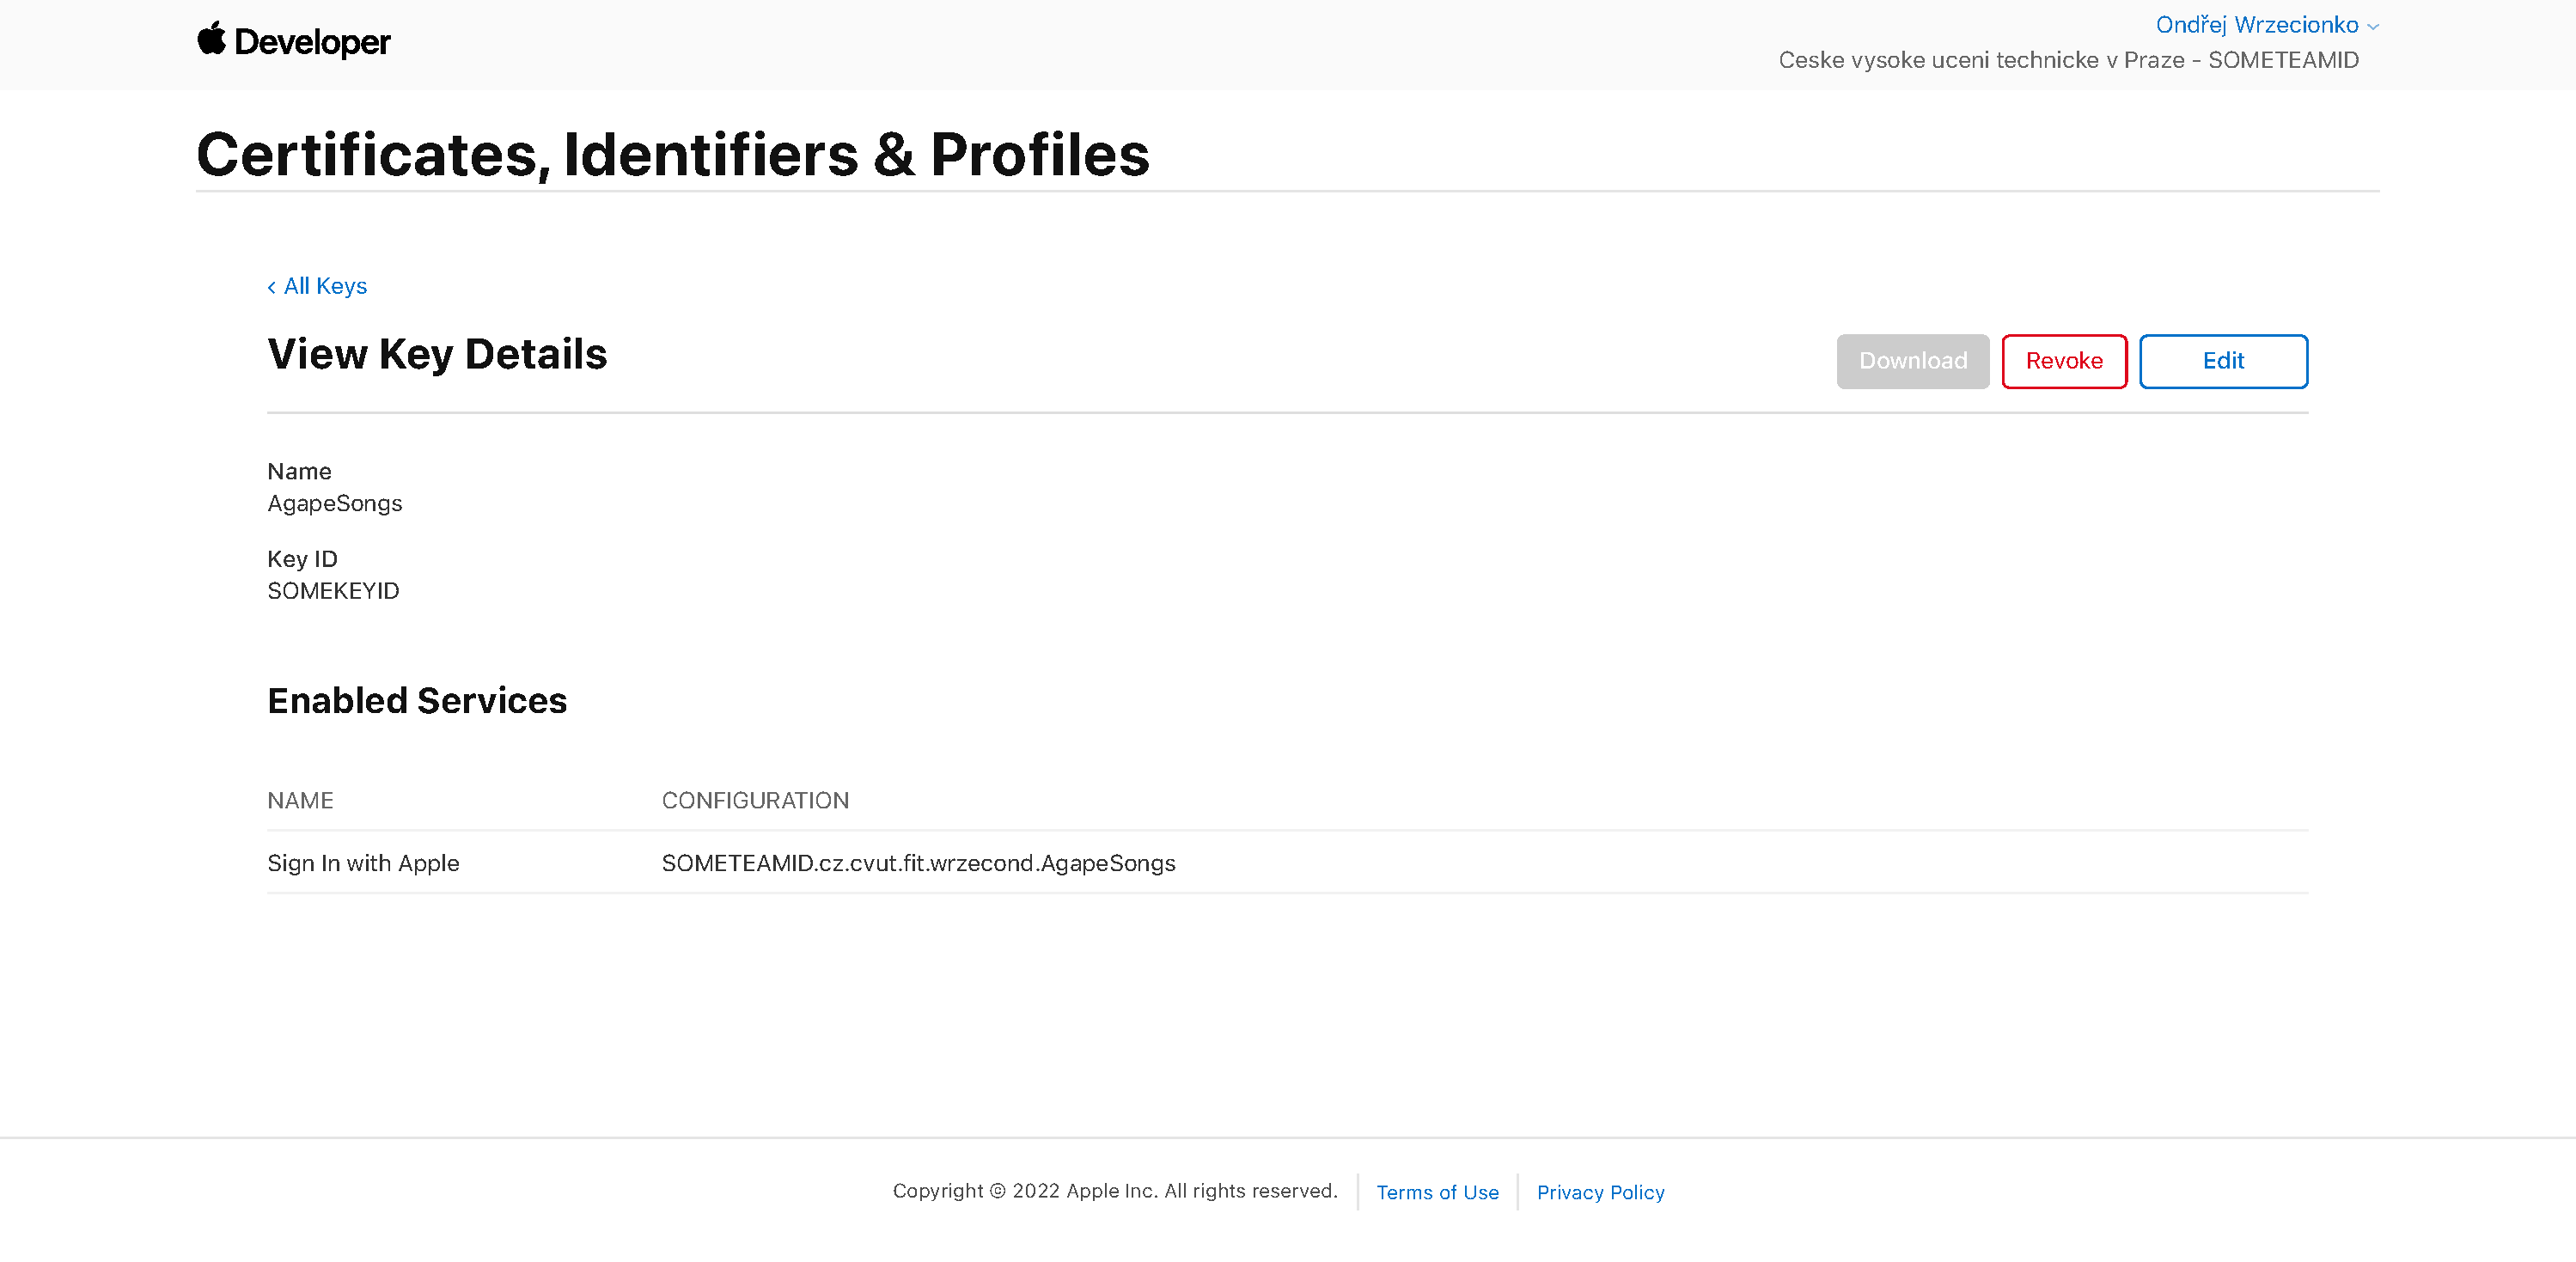
\includegraphics[width=\textwidth]{images/4-implementace/4-1-prihlaseni-pres-apple-klic.pdf}
    \caption{Apple vývojářský portál -- nastavení klíče pro Přihlášení přes Apple}
\end{figure}

Jak klíč, tak identifikátor aplikace nastavuji v konfiguračním souboru serveru, což je v případě frameworku Spring Web soubor \texttt{application.properties}, který je umístěn ve stejné složce jako výsledný server.

\begin{listing}[H]
\begin{minted}[breaklines,breaksymbolleft=]{properties}
auth.keyPath=/root/server/key.p8
auth.keyId=SOMEKEYID
auth.teamId=SOMETEAMID
\end{minted}
\caption{Ukázka konfiguračního souboru serveru \texttt{application.properties}}
\end{listing}

\begin{listing}[H]
\begin{minted}[breaklines,breaksymbolleft=]{kotlin}
// AuthService.kt
private fun appleAuth (code: String) : AppleUserInfo = tryCatch {
    val body  = networkService.appleAuthRequest(code, generateJWT())
    val token = Gson().fromJson(body, AppleToken::class.java)
    val payload = token.id_token.split(".")[1]
    val decoded = String(Decoders.BASE64.decode(payload))
    Gson().fromJson(decoded, AppleUserInfo::class.java)
}

private fun generateJWT () = Jwts.builder()
    .setHeaderParam(JwsHeader.KEY_ID, keyId)
    .setIssuer(teamId)
    .setAudience(APPLE_ENDPOINT)
    .setSubject(CLIENT_ID)
    // valid for 300 seconds
    .setExpiration(Date(300 * 1000 + System.currentTimeMillis()))
    .setIssuedAt(Date(System.currentTimeMillis()))
    .signWith(loadKeyFromFile(), SignatureAlgorithm.ES256)
    .compact()

// NetworkService.kt
@Service
class NetworkService {
    // Initiate HTTP client for network requests
    private val client = HttpClient(Java) {
        install(JsonFeature) {
            serializer = GsonSerializer {}
        }
    }

    fun appleAuthRequest (code: String, secret: String) : String = runBlocking {
        client.submitForm<HttpStatement>(
            url = AuthService.APPLE_ENDPOINT + AuthService.APPLE_PATH,
            formParameters = Parameters.build {
                append("client_id", AuthService.CLIENT_ID)
                append("client_secret", secret)
                append("grant_type", "authorization_code")
                append("code", code)
            }
        ).execute().receive()
    }
}
\end{minted}
\caption[Ukázka Service pro připojení k Apple serveru]{Třída \texttt{AuthService} při požadavku o přihlášení přes Apple vygeneruje JSON web token, který předá spolu s obdrženým kódem třídě  \texttt{NetworkService} komunikující s Apple serverem. Ta pak provede HTTP požadavek a vrátí informace o přihlášeném uživateli, které \texttt{AuthService} zpracuje a převede na informace o přihlášeném uživateli}
\end{listing}

%---------------------------------------------------------------
\chapter{Implementace mobilní aplikace}
%---------------------------------------------------------------

\begin{chapterabstract}
    V této kapitole popíšu průběh implementace mobilní aplikace, jednotlivé třídy a zajímavosti, se kterými jsem se při implementaci setkal.
\end{chapterabstract}

\section{Architektura}

Pro svou aplikaci jsem zvolil architekturu MVVM (Model View ViewModel). Aplikace se skládá ze tří vrstev -- datové, která obsahuje balíčky DTO s definicemi tříd z API, Service s třídami, které komunikují s API, business vrstvu, která obsahuje Modely s definicemi tříd, se kterými pracuje prezentační vrstva, ViewModely řešící veškerou logiku aplikace a prezentační vrstvu, která obsahuje View -- definici jednotlivých obrazovek aplikace a speciální třídu \texttt{AppState}, která zajišťuje kompatibilitu View používaných pro operační systém iOS a macOS.

\subsection{DTO}

Balíček DTO je ekvivalentem balíčku DTO na serveru. Tento balíček obsahuje definici dat, která aplikace získá z REST API. Ačkoliv jsou atributy DTO tříd na serveru a v mobilní aplikaci stejné, třídy nelze sdílet, jelikož jsou napsány v odlišných programovacích jazycích (Kotlin, Swift). Podobně jako na serveru, i v aplikaci má DTO různé typy -- základní \texttt{DTO} slouží k získávání informací z API, \texttt{EditDTO} slouží k vytváření a úpravě, \texttt{RawDTO} je zjednodušená verze základního DTO k zamezení cyklických závislostí a \texttt{SaveDTO} je určeno k uložení dat do cache v zařízení. Jednotlivá DTO implementují protokoly \texttt{Codable} \cite{swift-codable} (podporuje zakódování i dekódování), \texttt{Decodable} (podporuje pouze dekódování) nebo \texttt{Encodable} (podporuje pouze zakódování).

\begin{listing}[H]
\begin{minted}[breaklines,breaksymbolleft=]{swift}
struct SongBookDTO: Decodable {
    let id: Int
    let name: String
    let band: BandDTO
    let songs: [SongDTO]
}
struct SongBookEditDTO: Encodable {
    let name: String
    let bandId: Int
}
\end{minted}
\caption[Ukázka DTO zpěvníku v aplikaci]{Ukázka \texttt{SongBookDTO} ke čtení a \texttt{SongBookEditDTO} k úpravě}
\end{listing}

\subsection{Service}

Třídy z balíčku Service komunikují s API rozhraním za pomocí DTO a získaná data zpřístupňují ViewModelům. Jelikož je komunikace s API operace, při které probíhá přenos dat po síti, musí být metody, ve kterých probíhá komunikace s API asynchronní, aby během volání API metod nedošlo k zaseknutí uživatelského rozhraní.

Swift umožňuje volání asynchronních metod dvěma způsoby. Starší z nich využívá takzvaný \textit{completion handler}, což je funkce vyššího řádu, která je předána volající metodě jako parametr. Tato funkce se po provedení požadavku zavolá s datovým typem indikujícím úspěch, nebo chybu. Nový způsob \textit{Async API} umožňuje používat asynchronní funkce stejně jako synchronní s použitím klíčového slova \texttt{await}. Kód je tak přehlednější a srozumitelnější. \cite{swift-async-completion}

\begin{listing}[H]
\begin{minted}[breaklines,breaksymbolleft=]{swift}
func songBookList() async -> Result<[SongBookDTO], HttpStatusError> {
    let response = await networkService.get(url: Constants.songBookListUrl)
    switch response {
    case .success(let data):
        guard let songBooks = try? JSONDecoder().decode(
            [SongBookDTO].self, from: data
        ) else {
            return .failure(.badtext(
                text: "songbook_list_response_parse_error"
            ))
        }
        return .success(songBooks)
    case .failure(let error):
        return .failure(error)
    }
}
\end{minted}
\caption[Ukázka Service pro zpěvníky v aplikaci]{Ukázka metody \texttt{songBookList}, která na API odešle požadavek na získání seznamu zpěvníků. V případě úspěšného provedení požadavku se z odpovědi pokusí načíst pole DTO zpěvníků, v~případě neúspěchu pak vrátí příslušnou chybu}
\end{listing}

\subsection{Model}

Balíček Model obsahuje definici jednotlivých entit, se kterými se pracuje v aplikaci. Pro převod mezi entitami a příslušnými DTO (ať už základními, pro úpravu nebo uložení do cache) jsou použity \textit{extension properties} \cite{swift-extensions}, které umožňují přidat nové atributy do libovolné třídy bez nutnosti její úpravy. Balíček DTO jakožto součást datové vrstvy tak neobsahuje metody pro převod na jednotlivé Modely, čímž je zachována třívrstvá architektura.

\begin{listing}[H]
\begin{minted}[breaklines,breaksymbolleft=]{swift}
struct SongBook: Equatable {
    let id: Int
    let name: String
    let band: Band
    let songs: [Song]
}
\end{minted}
\caption{Ukázka Modelu zpěvníku v aplikaci}
\end{listing}

\subsection{ViewModel}

ViewModely jsou třídy, které komunikují s příslušnými třídami z balíčku Service a drží Modely, se kterými dále pracují komponenty z balíčku View. Ve ViewModelech je obsažena veškerá logika pro zpracovávání operací včetně logiky pro vytváření, úpravu, smazání nebo zobrazování dat.

\begin{listing}[H]
\begin{minted}[breaklines,breaksymbolleft=]{swift}
final class SongBookListViewModel: ObservableObject {
    @Published var state: SongBookListLoadState = .loading
    @Published var songBooks = [SongBook]()
    @Published var songsById = [String: Song]()
    
    func loadSongBooks() {
        state = .loading
        Task { await loadSongBooks() }
    }
    
    func loadSongBooks() async {
        let songBooks = await songBookService.songBookList()
        await loadSongBooks(result: songBooks)
    }
    
    @MainActor
    private func loadSongBooks(result: Result<[SongBookDTO], HttpStatusError>) async {
        switch result {
        case .success(let songBooks):
            self.songBooks = songBooks.map { song -> song.domain }
            songsById = [:] // reset song book list
            songsById = self.songBooks.flatMap { songBook -> songBook.songs }.reduce(into: songsById) { song ->
                songBook[song.idString] = song
            }
            
            appState.songBook = self.songBooks.first(where: { songBook -> songBook.id == appState.songBook?.id })
            state = .success
        case .failure(let error):
            state = .failure(error.errorDescription)
        }
    }
}
\end{minted}
\caption[Ukázka kódu z ViewModelu pro načtení seznamu zpěvníků v aplikaci]{Ukázka kódu ze \texttt{SongBookListViewModelu}, který slouží pro načtení seznamu zpěvníků a jeho zpřístupnění komponentě \texttt{SongBookListView}, která je zobrazí uživateli. Na začátku jsou definovány proměnné držící stav načítání, seznam zpěvníků a slovník písní podle jejich unikátního identifikátoru. Samotné načtení pak zajišťuje metoda  \texttt{loadSongBooks}, kde první varianta (bez klíčového slova \texttt{async}) zajistí spuštění druhé metody v asynchronním kontextu pomocí třídy \texttt{Task}, druhá varianta (s \texttt{async}) zajistí zavolání příslušné metody na \texttt{SongBookService} a poslední metoda (označená \texttt{@MainActor}) manipuluje s daty, na která je napojena komponenta View -- proto je zde použita anotace \texttt{@MainActor}, která zajistí spuštění metody na hlavním jádře}
\end{listing}

\subsection{View}

View je balíček, který obsahuje definici jednotlivých SwiftUI komponent, které tvoří uživatelské rozhraní. Tyto komponenty drží příslušný ViewModel a další pomocné proměnné, pomocí kterých je deklarativně určena aktuální podoba rozhraní.

\begin{listing}[H]
\begin{minted}[breaklines,breaksymbolleft=]{swift}
struct SongBookListView: View {
    @ObservedObject var songBookListViewModel: SongBookListViewModel

    var body: some View {
        VStack {
            switch songBookListViewModel.state {
            case .loading:
                ProgressView()
            case .failure(let error):
                ErrorView(error: error, action: songBookListViewModel.loadSongBooks, dismiss: nil)
            case .success:
                SongBookListWrapperView(songBookListViewModel: songBookListViewModel)
            }
        }
    }
}
\end{minted}
\caption[Ukázka komponenty pro zobrazení seznamu písní v aplikaci]{Ukázka komponenty \texttt{SongBookListView} pro zobrazení seznamu písní -- na základě stavu načítání z příslušného \texttt{SongBookListViewModel}u je zobrazeno buď \texttt{ProgressView} (načítací obrazovka), \texttt{ErrorView} (obrazovka zobrazující příslušnou chybovou hlášku \texttt{error} s akcemi pro znovunačtení \texttt{action} a zrušení \texttt{dismiss}), nebo obrazovka \texttt{SongBookListWrapperView} obalující seznam zpěvníků na~operačních systémech macOS a iOS.}
\end{listing}

\section{Multiplatformní aplikace}

Na základě návrhu jsem mobilní aplikaci implementoval jako nativní aplikaci pro operační systémy iOS a macOS pomocí technologie Swift. Celá aplikace je tedy rozdělena do tří částí -- \texttt{Shared}, která obsahuje sdílenou logiku a částí \texttt{macOS} a \texttt{iOS}, které každá obsahují logiku specifickou pro danou platformu.

\subsection{Uživatelské rozhraní}

Pro tvorbu uživatelského rozhraní mobilní aplikace jsem si mohl zvolit dva základní systémy tvorby rozhraní iOS / macOS aplikací. Prvním z nich jsou systémy UIKit (iOS) \cite{uikit} a AppKit (macOS) \cite{appkit}. Jedná se o specifické systémy pro tvorbu rozhraní na jednotlivé platformy. Jejich výhodou je především univerzálnost -- dá se v nich napsat bez problému jakákoliv obrazovka. Druhým je pak nový systém SwiftUI \cite{swiftui}, který je společný pro obě platformy. Není sice tak univerzální jako UIKit nebo AppKit -- při vývoji se tak může stát, že je nutné některou obrazovku napsat v těchto systémech, jeho výhodou je ale multiplatformnost -- jednou napsaný kód funguje na obou platformách.

Při tvorbě designu aplikace jsem narazil na komponenty, které nebylo možné implementovat pomocí SwiftUI. Jednalo se o seznam písní a zpěvníků, dialogy a navigační lištu.

\subsubsection{Seznam písní a zpěvníků}

Pro vytvoření seznamu prvků se ve SwiftUI používá komponenta \texttt{List} \cite{swiftui-list}. Této komponentě se předá seznam prvků a funkce, která z daného prvku vytvoří komponentu řádku seznamu. Zatímco na iOS tato komponenta obstarává posouvání seznamu, odsazení od krajů, hledání v~seznamu a rozdělení do sekcí (zpěvníků), na macOS jsou tyto funkcionality nefunkční. V seznamu na macOS navíc není funkční posouvání po prvcích pomocí šipek na klávesnici. Seznam písní a zpěvníků jsem tak musel na platformě macOS implementovat vlastním řešením s pomocí SwiftUI komponenty \texttt{LazyVStack} \cite{swiftui-lazyvstack}, která pouze vykreslí předané prvky pod sebe. Logiku posouvání seznamu, odsazení od krajů, hledání v seznamu a posouvání pomocí šipek jsem pak implementoval pomocí technologie UIKit.

\begin{figure}[H]
    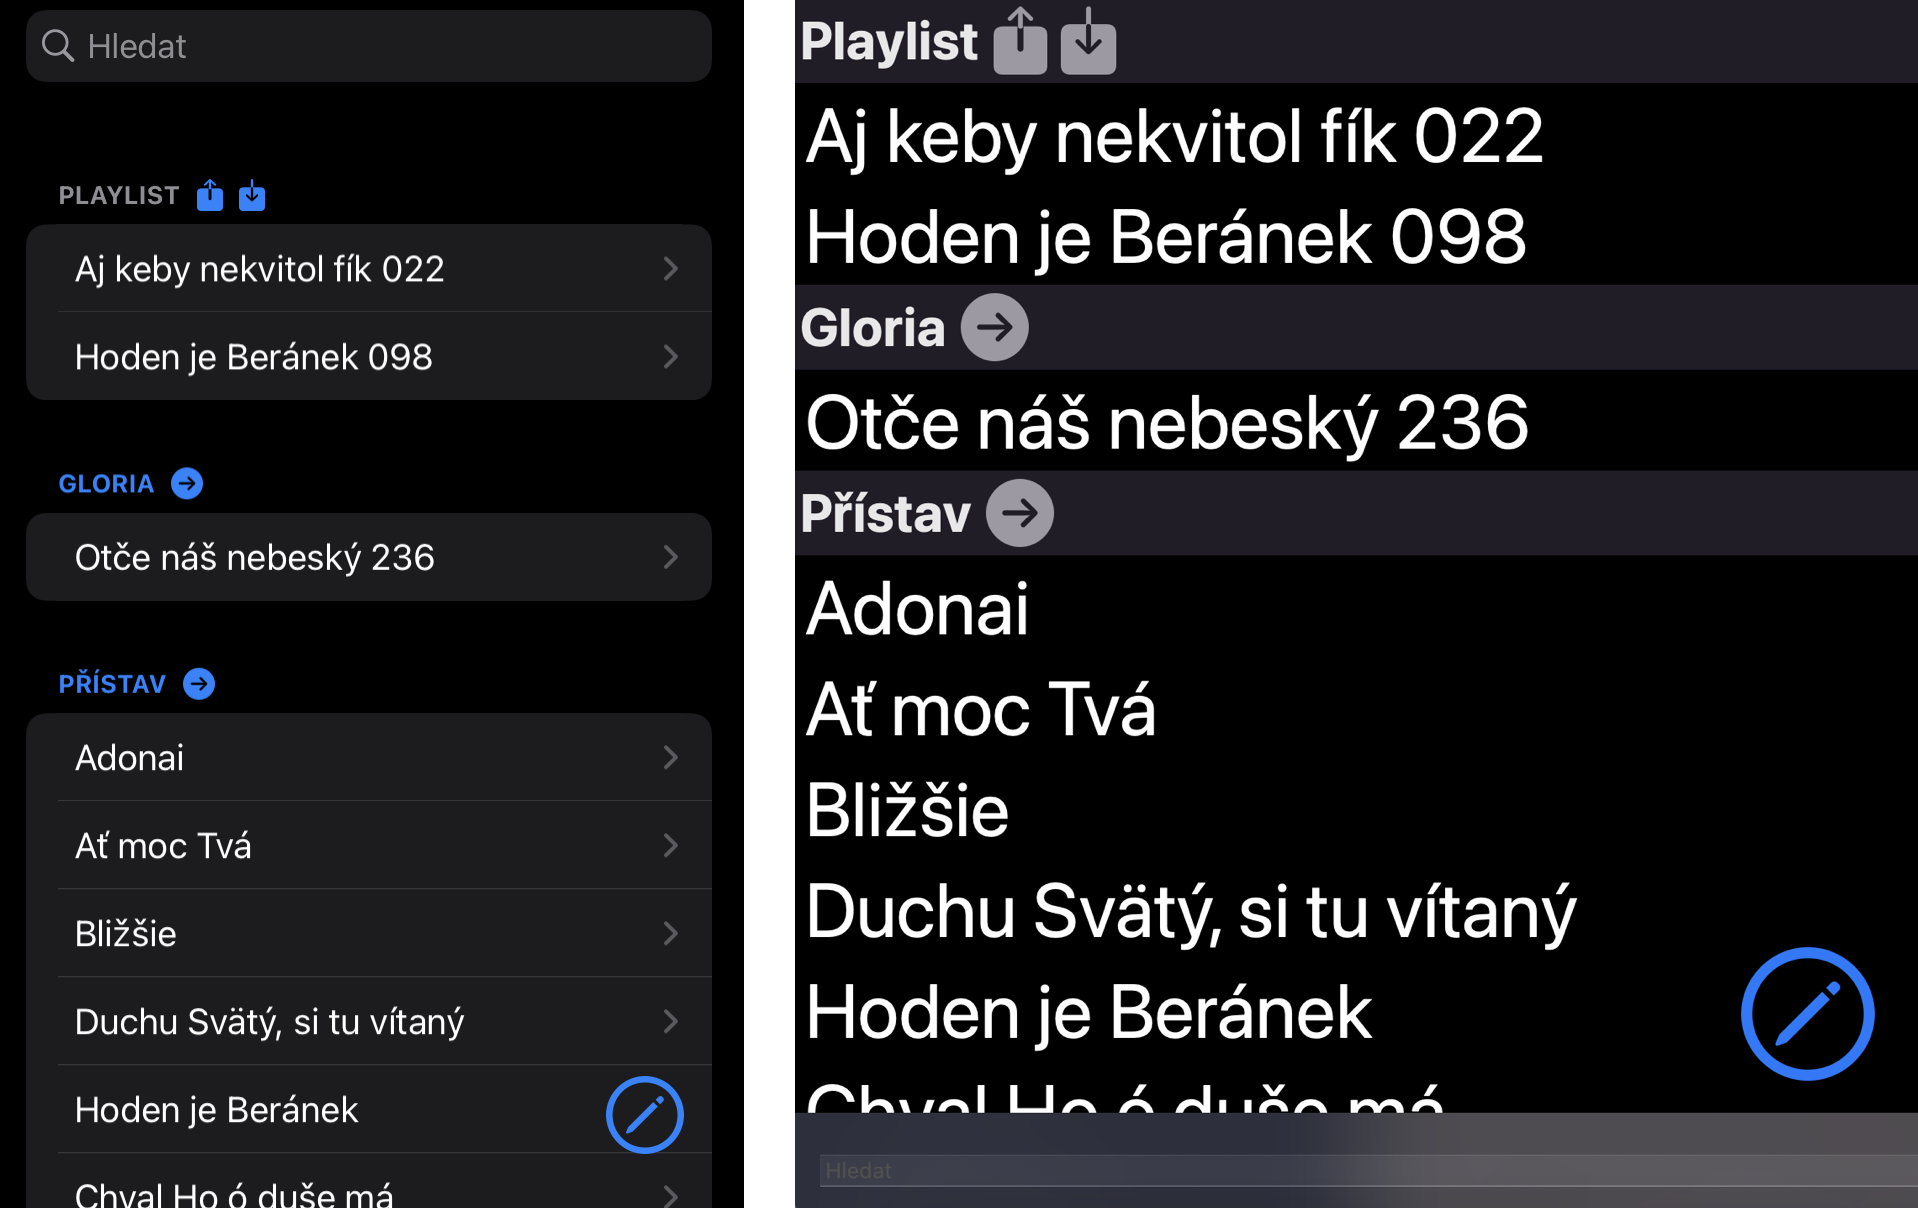
\includegraphics[width=\textwidth]{images/5-implementace/5-1-seznam-zpevniku.png}
    \caption[Seznam písní a zpěvníků -- rozdíl mezi iOS a macOS]{Seznam písní a zpěvníků -- vlevo nativní \texttt{List} řešení na systému iOS, vpravo vlastní řešení pro systém macOS s využitím SwiftUI komponenty \texttt{LazyVStack}}
\end{figure}

\subsubsection{Dialogy a navigační lišta}

Jelikož je iOS operační systém pro mobilní zařízení, zatímco macOS pro notebooky a počítače, je nativní chování prvků v navigační liště odlišné. Zatímco macOS podporuje v navigační liště tlačítka jak vlevo, tak vpravo, u iOS můžou být tlačítka přítomna pouze vpravo, jelikož se vlevo ukazuje nativní tlačítko pro návrat na předchozí obrazovku. Toto tlačítko pro návrat na předchozí obrazovku pak musí být v systému macOS tam, kde je potřeba (narozdíl od systému iOS totiž není povinné pro každou obrazovku), implementováno samostatně.

\begin{figure}[H]
    
\includegraphics[width=\textwidth]{images/5-implementace/5-2-navigacni-lista.png}
    \caption[Navigační lišta -- rozdíl mezi iOS a macOS]{Navigační lišta -- vlevo iOS s nativním tlačítkem pro návrat na obrazovku seznam zpěvníků, vpravo macOS s tlačítkem pro navigaci do nastavení. Na obou platformách je pak vpravo tlačítko pro zobrazení \texttt{popover} dialogu pro nastavení písně}
\end{figure}

Také způsob zobrazování dialogů na jednotlivých platformách je odlišný -- na macOS se typ dialogu \texttt{sheet} zobrazuje jako nové okno, nativně ale neobsahuje tlačítko pro zavření. Tlačítka se mu tak musí předat do navigační lišty s umístěním dolů. Na iOS je \texttt{sheet} dialog možné schovat potáhnutím prstu dolů, tlačítko pro odeslání je pak umístěno v navigační liště nahoře.

\begin{figure}[H]
    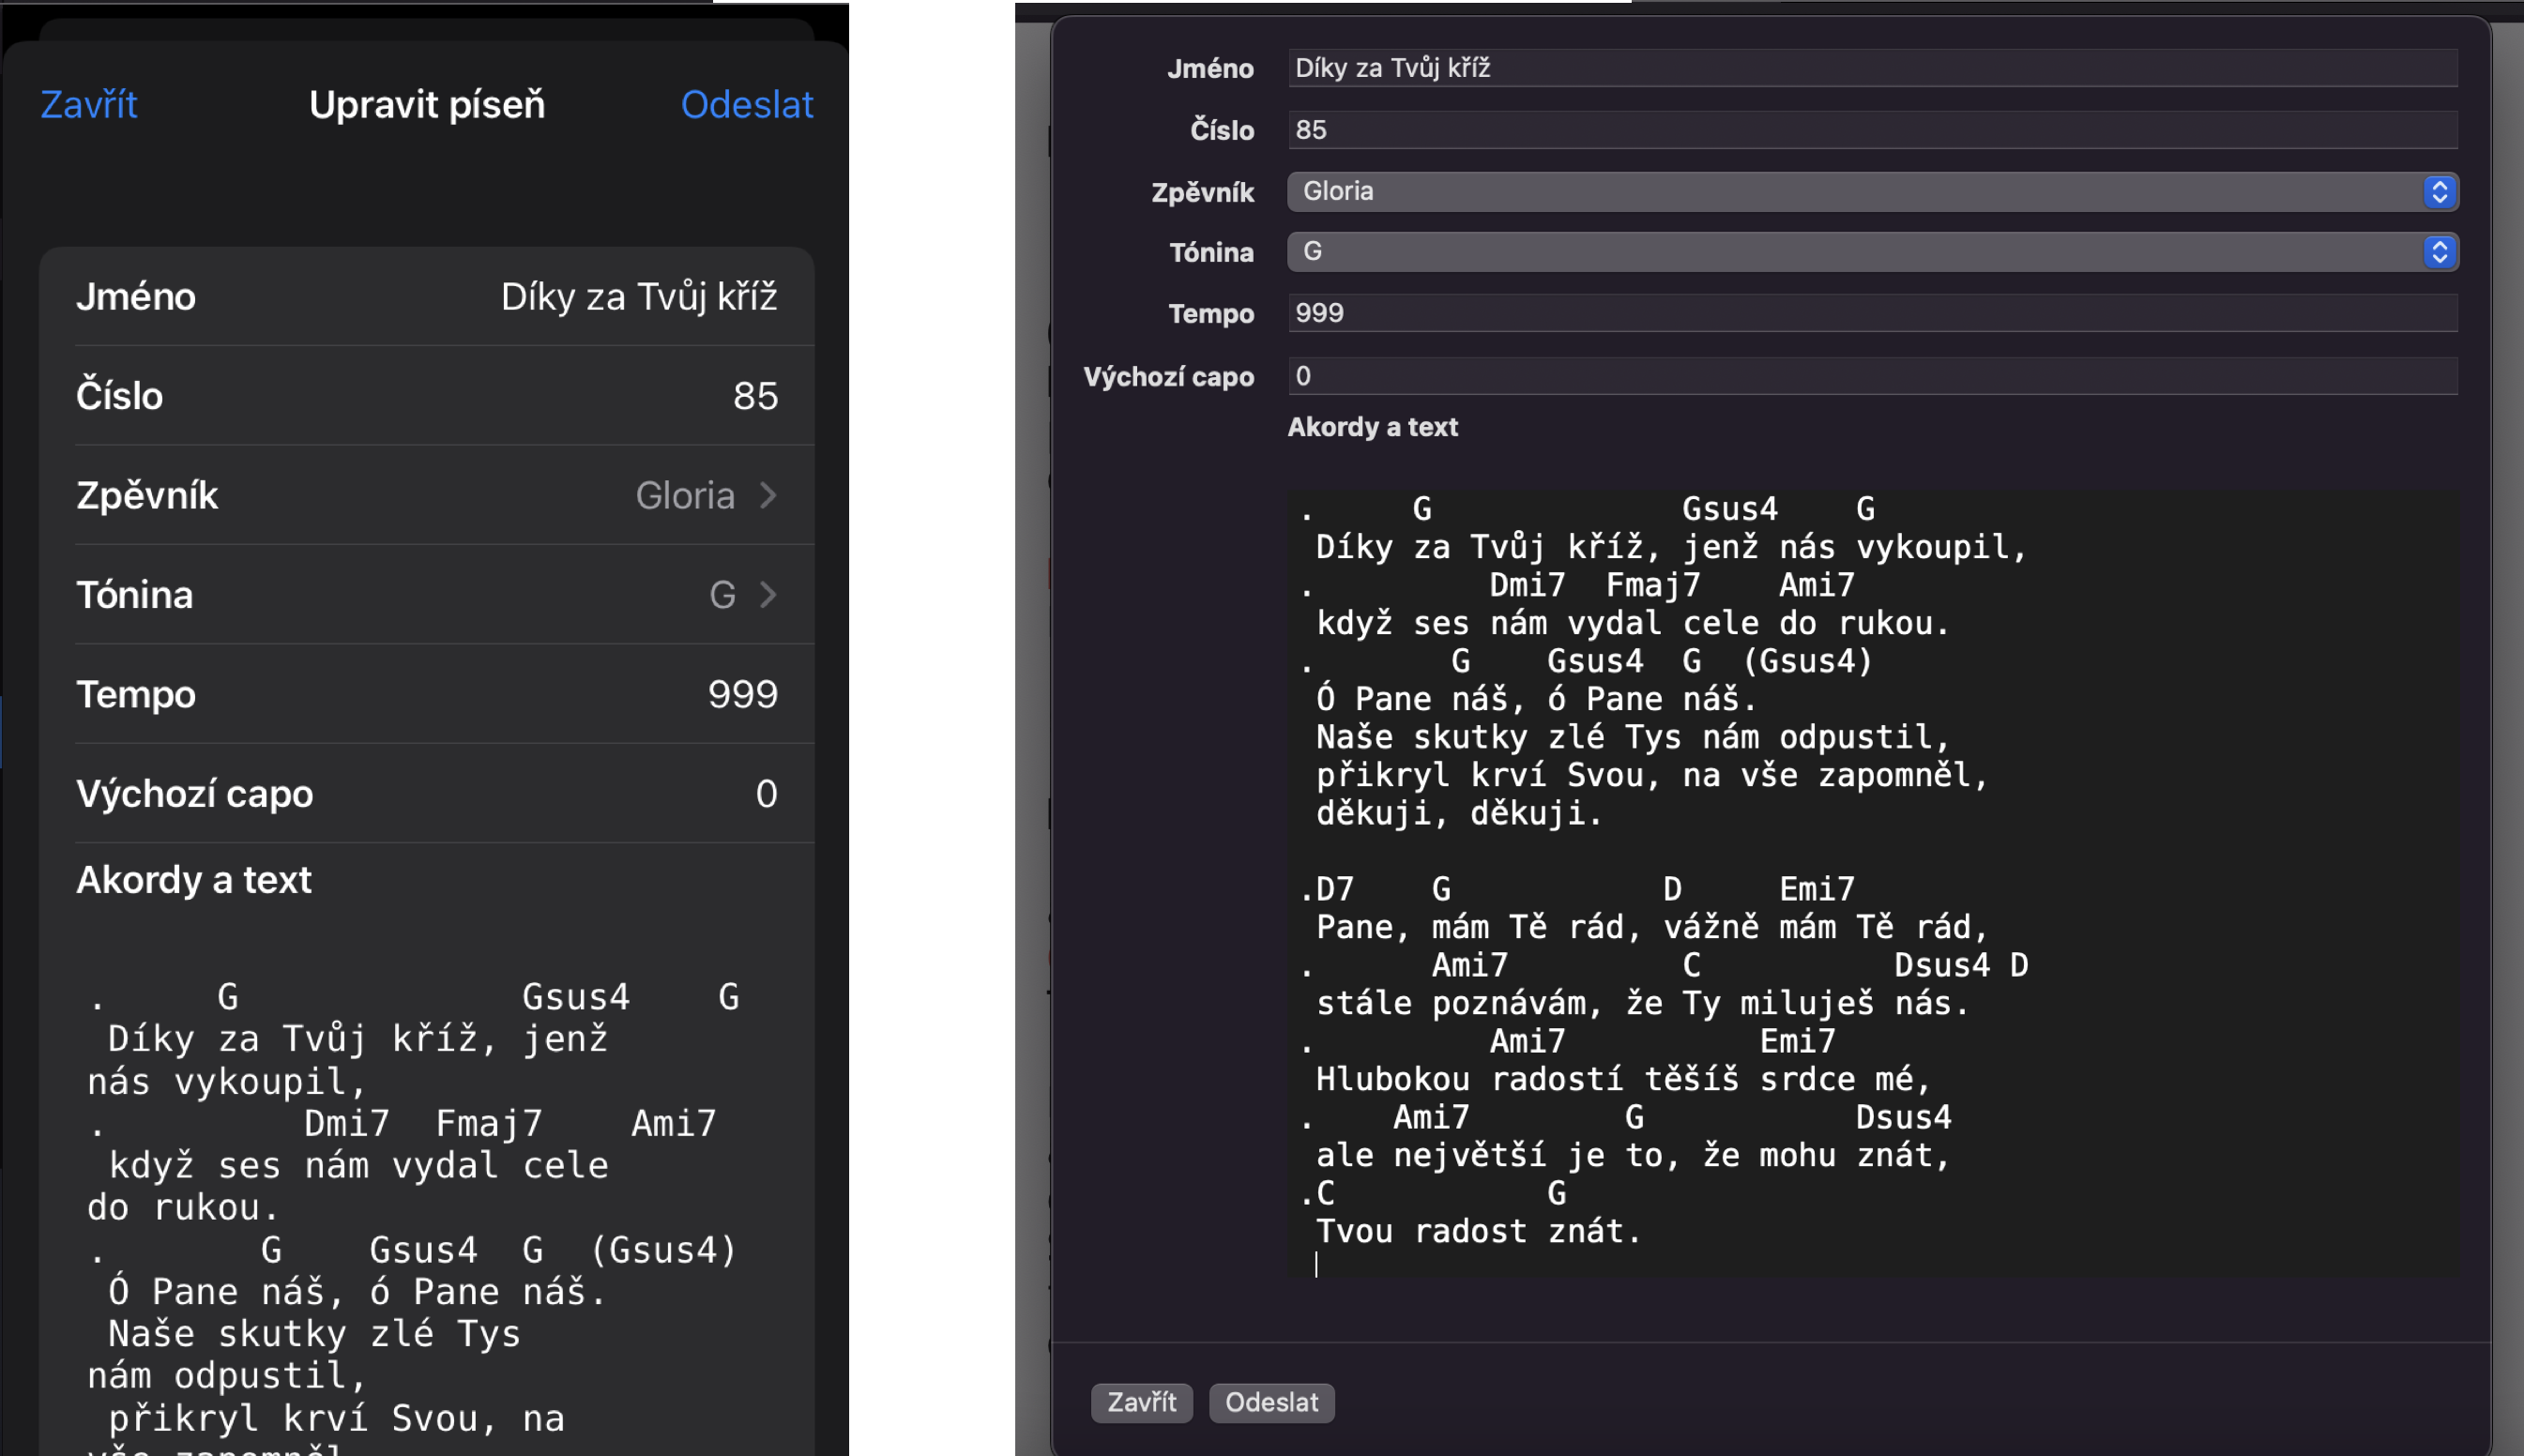
\includegraphics[width=\textwidth]{images/5-implementace/5-3-dialog-sheet.png}
    \caption[Úprava písně -- rozdíl mezi iOS a macOS]{Úprava písně -- vlevo iOS \texttt{sheet} dialog přes celou obrazovku s tlačítky nahoře a možností zavřít potáhnutím dolů, vpravo macOS \texttt{sheet} dialog jako nové okno s tlačítky dole v navigační liště}
\end{figure}

\subsection{Navigační logika}

Jak v iOS, tak v macOS aplikacích funguje navigace odlišně. V iOS aplikaci se používá způsob navigace \texttt{stack} -- uživatel vždy vidí právě jednu obrazovku, zatímco v macOS aplikaci je povinný způsob navigace \texttt{columns} -- uživatel vidí dva sloupce, kdy v levém je typicky seznam prvků a v~pravém detail prvku. Toto chování nativně zajišťuje komponenta \texttt{NavigationView} \cite{swiftui-navigationview}, které lze na základě platformy nastavit způsob navigace. Přechod mezi obrazovkami pak aplikace provádí pomocí komponenty \texttt{NavigationLink} \cite{swiftui-navigationlink}.

Při použití komponenty \texttt{NavigationView} a \texttt{NavigationLink} na systému iOS vše fungovalo správně. Když jsem ale tyto komponenty použil na systému macOS, detaily písní, které se měly zobrazovat v pravém sloupci, náhodně mizely. Pro macOS jsem tedy musel vytvořit vlastní řešení, které v rámci komponenty \texttt{NavigationView} zajišťuje přechod mezi obrazovkami bez použití komponenty \texttt{NavigationLink}.

\section{Dependency Injection}

Ve Swiftu sice existují externí frameworky řešící Dependency Injection, jejich použití je ale zbytečně příliš komplexní, proto jsem se rozhodl pro použití čistého Swift řešení \textit{protocol-oriented programming} \cite{protocol-oriented-programming}. Každá Service implementuje protokol \texttt{Servicing}, na kterém jsou závislé jednotlivé ViewModely. V celé aplikaci je pak k dispozici třída \texttt{DI}, které jsou předány jednotlivé Services pomocí \textit{extension property} a protokolu \texttt{HasServicing}.

\begin{listing}
\begin{minted}[breaklines,breaksymbolleft=]{swift}
// ContentView.swift
NavigationView {
    SongBookListView(songBookListViewModel: songBookListViewModel)
    if let song = appState.song { SongView(song: song) }
    else { Text("no_song_selected") }
}.navigationViewStyle(.columns)

// SongBookListView.swift
songListView.onTapGesture { appState.song = song }
\end{minted}
\caption[Navigační logika aplikace v systému macOS]{Navigační logika aplikace v systému macOS -- v \texttt{NavigationView} je jako první (zobrazí se vlevo) vždy komponenta pro seznam zpěvníků a pokud je ve třídě \texttt{AppState} nastavena aktuální píseň, zobrazí se její detail, jinak se zobrazí text informující uživatele o tom, že žádná píseň nebyla vybrána}
\end{listing}

\begin{listing}
\begin{minted}[breaklines,breaksymbolleft=]{swift}
// ContentView.swift
NavigationView {
    SongBookListView(songBookListViewModel: songBookListViewModel)
}.navigationViewStyle(.stack)

// SongBookListView.swift
NavigationLink(
    destination: SongView(songBook: songBook),
    tag: song.idString,
    selection: songBookViewModel.selectedSongId
) { songListView }
\end{minted}
\caption[Navigační logika aplikace v systému iOS]{Navigační logika aplikace v systému iOS -- v \texttt{NavigationView} je pouze komponenta pro seznam zpěvníků, přechod na detail písně provádí systém pomocí komponenty \texttt{NavigationLink}}
\end{listing}

\begin{listing}
\begin{minted}[breaklines,breaksymbolleft=]{swift}
// SongBookService.swift
protocol SongBookServicing {
    func songBookList() async -> Result<[SongBookDTO], HttpStatusError>
}
protocol HasSongBookService {
    var songBookService: SongBookServicing { get }
}

private let _songBookService = SongBookService(context: context)
extension DI: HasSongBookService {
    var songBookService: SongBookServicing { _songBookService }
}

// SongBookListViewModel.swift
private let songBookService: SongBookServicing
init(context: HasSongBookService) {
    songBookService = context.songBookService
}
\end{minted}
\caption[Ukázka použití protocol-oriented programming v aplikaci]{Ukázka použití protocol-oriented programming ve třídě Service pro zpěvníky, která dědí z protokolu \texttt{SongBookServicing}, na kterém závisí ViewModel pro seznam písní. Předání \texttt{SongBookService} do ViewModelu pak probíhá pomocí třídy \texttt{DI}.}
\end{listing}

\section{Dělení textu písně}

Při programování obrazovky detailu písně jsem se nečekaně setkal s problémem při zalamování textu a akordů písně. Při použití nativní SwiftUI komponenty \texttt{Text} \cite{swiftui-text} se jinak zalamovaly řádky s akordy a jinak řádky s textem. Toto zalomení způsobilo nesprávnou polohu akordů vůči jednotlivým slovům textu, což činilo aplikaci nepoužitelnou na menších zařízeních s větší velikostí textu.

\begin{figure}[H]
    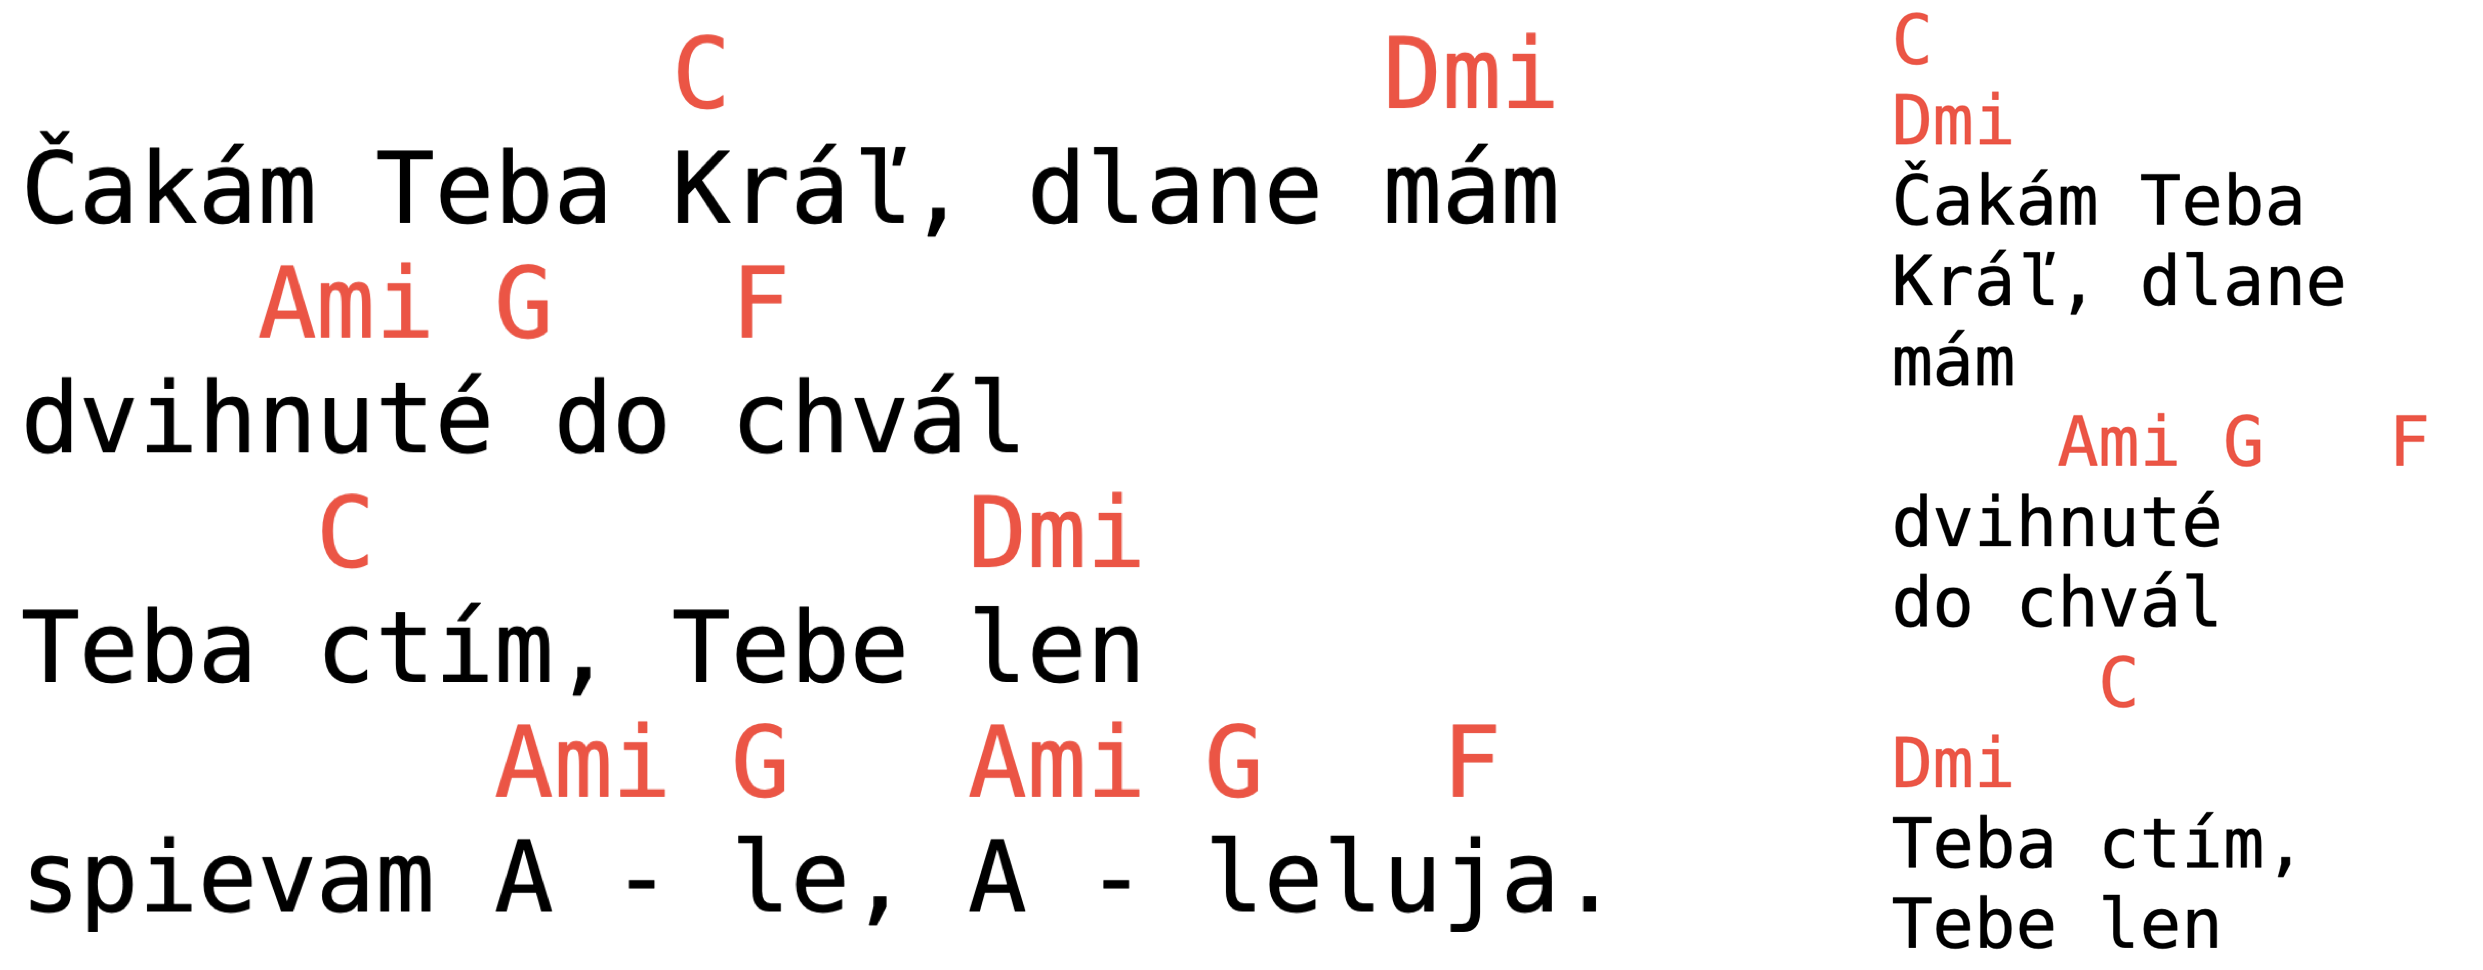
\includegraphics[width=\textwidth]{images/5-implementace/5-4-spatne-zalomeni.png}
    \caption[Ukázka nesprávného zalamování textu v detailu písně]{Ukázka nesprávného zalamování textu v detailu písně -- vlevo je původní text, vpravo nesprávně zalomený text -- akordy jsou v nesprávné poloze}
\end{figure}

Při průzkumu stávajících řešení zalamování textu jsem zjistil, že pro technologii SwiftUI aktuálně narozdíl od jiných technologií jako je CSS neexistuje nativní řešení ani jednoduše použitelná knihovna, která by umožnila text správně zalomit. Rozhodl jsem se proto implementovat vlastní algoritmus, který text rozdělí na základě maximálního možného počtu znaků, které se vejdou na obrazovku na šířku a jelikož neexistuje nativní řešení ani knihovna pro zjištění tohoto maximálního počtu znaků, implementoval jsem také jeho výpočet.

\begin{figure}[H]
    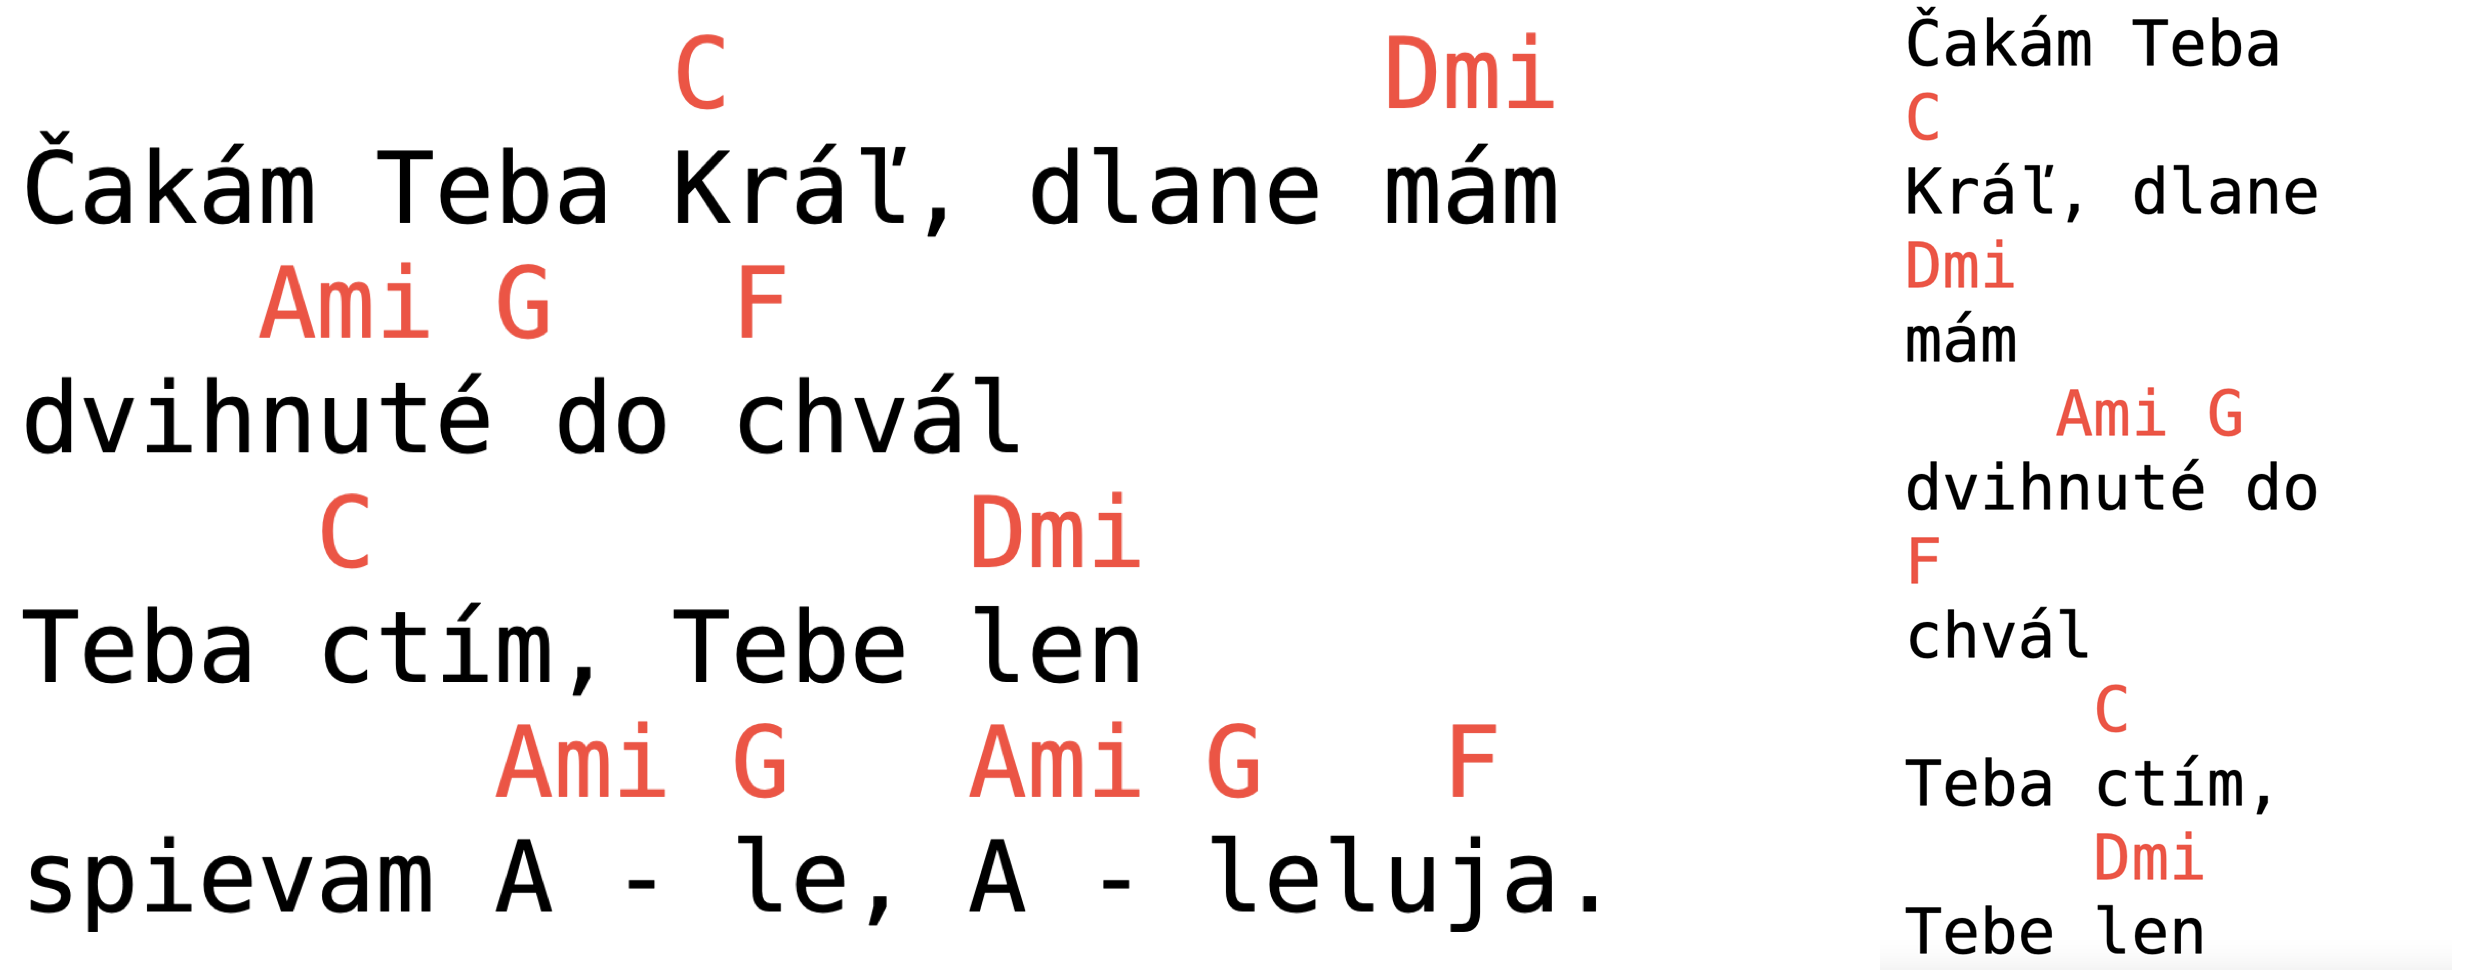
\includegraphics[width=\textwidth]{images/5-implementace/5-5-spravne-zalomeni.png}
    \caption[Ukázka správného zalamování textu v detailu písně]{Ukázka správného zalamování textu v detailu písně -- vlevo je původní text, vpravo zalomený text -- je zachována poloha všech akordů}
\end{figure}

Dělení textu tak, aby bylo na řádce maximálně N znaků pak probíhá algoritmicky nalezením poslední pozice v prvních N znacích, na které je jak v akordech, tak v textu mezera. Pokud taková pozice neexistuje, text je rozdělen po N znacích bez ohledu na mezery.

\begin{listing}
\begin{minted}[breaklines,breaksymbolleft=]{swift}
// SongWidthReaderView.swift
struct SongWidthReaderView<Content>: View where Content: View {
    @ObservedObject var songViewModel: SongViewModel
    let content: (Int) -> Content
    
    var body: some View {
        ZStack {
            ScrollView {
                VStack {
                    if let maxChars = songViewModel.maxLineChars {
                        HStack {
                            content(maxChars)
                            Spacer()
                        }
                    }
                    
                    Text("X")
                        .hidden()
                        .font(.custom(
                            "Bitstream Vera Sans Mono",
                            size: songViewModel.textSize
                        ).monospaced())
                        .readWidth(songViewModel.textWidth)
                }
            }
        }
        .readWidth(songViewModel.viewWidth)
    }
}

// SongViewModel.swift
@Published var maxLineChars: Int? = nil

@Published var textWidth: Double? = nil {
    didSet { calculateMaxLineChars() }
}

@Published var viewWidth: Double? = nil {
    didSet { calculateMaxLineChars() }
}

private func calculateMaxLineChars() {
    guard let textWidth = textWidth, let viewWidth = viewWidth else { return }
    maxLineChars = Int(viewWidth / textWidth)
}
\end{minted}
\caption[Ukázka pomocné třídy pro zalamování textu v aplikaci]{Třída \texttt{SongWidthReaderView} počítá maximální počet znaků, které se vejdou na obrazovku jako šířku celé obrazovky (metoda \texttt{readWidth} na komponentě \texttt{ZStack}) dělenou šířkou jednoho znaku (metoda \texttt{readWidth} na komponentě \texttt{Text}, která je skrytá metodou \texttt{hidden}). Jakmile je přečtena šířka obrazovky i znaku, je nastaven maximální počet znaků a předán komponentě \texttt{content}, která správně rozdělí text a akordy písně a zobrazí je uživateli}
\end{listing}

\section{Transpozice}

Jednou z častých úprav akordů, kterou členové hudebního doprovodu provádí, je takzvaná \textit{transpozice akordů}. Jedná se o posun akordů z jedné tóniny do jiné o daný počet půltónů. Tento posun se provádí z různých důvodů, mezi nejčastější z nich patří usnadnění zpěvu nebo hry na nástroj. \cite{transpozice}. Problémem ale je, že každý hudebník nepoužívá stejnou transpozici -- například klavírista hraje v originální tónině, zatímco kytarista použije transpozici -3 a nasadí kapodastr na třetí pražec. V aplikaci jsem se proto rozhodl transpozici umožnit a nazval jsem ji \textit{capo} (z anglického capodastr).

\begin{figure}[H]
    \centering
    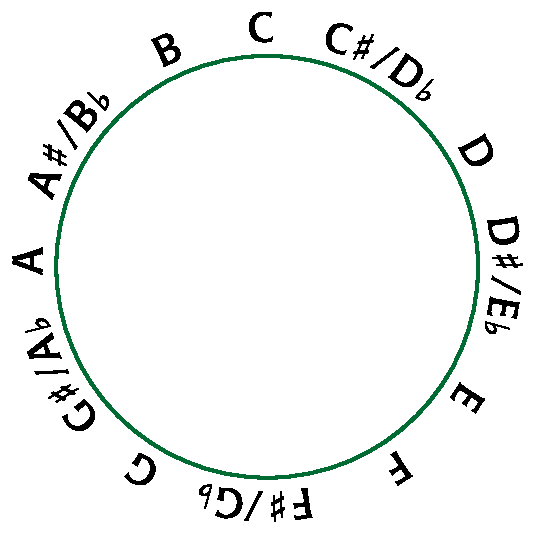
\includegraphics[width=0.6\textwidth]{images/5-implementace/5-6-chromaticky-kruh.pdf}
    \caption[Chromatický kruh znázorňující posloupnost akordů při transpozici]{Chromatický kruh znázorňující posloupnost 12 akordů při transpozici \cite{chromatic-circle}}
\end{figure}

Algoritmická transpozice akordů probíhá vytvořením pole všech 12 tónin. Pro každý akord v~textu je nalezena jeho tónina, index této tóniny v poli tónin a k tomuto indexu je přičten nebo odečten počet půltónů. Na výsledném indexu se pak nachází transponovaný akord.

\begin{listing}[H]
\begin{minted}[breaklines,breaksymbolleft=]{swift}
let transposed = original.map { chord -> (String, String) in
    for key in SongKey.allCases {
        let transposed = key.transpose(steps: capo, keys: keys)
        if chord.replacingOccurrences(of: "(", with: "").starts(with: key.localized) {
            return (chord, chord.replacingOccurrences(of: key.localized, with: transposed.localized))
        }
    }
    return (chord, chord)
}
\end{minted}
\caption{Ukázka algoritmu pro transpozici akordů}
\end{listing}

Při takovéto transpozici jsem musel řešit dva problémy. Prvním problémem je různé značení jednotlivých tónin -- například tónina C\musSharp{} dur je pro účely aplikace ekvivalentní s tóninou D\musFlat{} dur. V aplikaci jsem tedy do nastavení přidal možnost volby, zda se mají akordy transponovat podle původní tóniny písně, nebo se mají použít vždy křížky/béčka.

\begin{listing}[H]
\begin{minted}[breaklines,breaksymbolleft=]{swift}
var skip = 0
let result = transposed.compactMap { pair -> String? in
    let originalStr = pair.0, transposedStr = pair.1

    // Odstranění přebytečných mezer
    if skip > 0 && transposedStr.isEmpty {
        skip -= 1
        return nil
    }
    
    // OK, transpozice nemění počet znaků
    if originalStr.count == transposedStr.count {
        return transposedStr
    }
    
    // Počet znaků je nyní menší = přidáme mezeru
    if transposedStr.count < originalStr.count {
        return transposedStr + " "
    }
    
    // Počet znaků je větší, zvětšíme rozdíl
    skip += 1
    return transposedStr
}
\end{minted}
\caption{Ukázka algoritmu, který po transpozici opraví polohu akordů vůči textu}
\end{listing}

Druhý problém je způsoben rozdílnou délkou akordů během transpozice -- například akord C má jeden znak a C\musSharp{} má 2 znaky, což způsobuje, že se při transpozici mění poloha akordů vůči textu. Tento problém jsem vyřešil tak, že si při transpozici akordů pamatuji také původní akord a po transpozici všech akordů projdu postupně všechny akordy na řádku a pamatuji si rozdíl mezi počtem znaků transponovaných akordů a původních akordů. Kdykoliv se pak mezi akordy objeví více než jedna mezera, smažu přebytečné mezery s cílem zachování původní polohy akordů.

\section{Lokalizace}

Jedním z nefunkčních požadavků na aplikaci je podpora češtiny a polštiny. SwiftUI lokalizaci nativně podporuje -- pokud je do nativní komponenty předán textový řetězec, pokusí se ho nejprve najít v lokalizační tabulce \texttt{Localizable.strings} jazyka, který uživatel zvolil pro aplikaci, případně jazyka systému. Pokud tento řetězec v dané tabulce existuje, je přeložen, jinak je jako text použit klíč samotný. SwiftUI komponenty ale nativně nepřekládají texty, které jsou do nich vloženy v proměnných. Takové texty musí být přeloženy manuálně voláním makra \texttt{NSLocalizedString} \cite{swift-localizedstring}.

%---------------------------------------------------------------
\chapter{Testování}
\label{testovani}
%---------------------------------------------------------------

\begin{chapterabstract}
    V této kapitole otestuji naprogramovaný server, REST API a mobilní aplikaci pomocí automatizovaných a uživatelských testů. Následně opravím chyby, které zjistím v průběhu automatizovaných testů a zapracuji zpětnou vazbu z uživatelských testů.
\end{chapterabstract}

Po naprogramování první verze aplikace před jejím samotným vypuštěním na trh je vhodné aplikaci řádně otestovat. Existují dva základní typy testů, které lze použít k testování -- automatizované testy a uživatelské testy. Server, REST API i mobilní aplikaci jsem průběžně testoval pomocí automatizovaných i uživatelských testů.

\section{Automatizované testy}

Automatizované testy jsou takové, které programátor jednou napíše a spouští se automaticky, například při každém odeslání kódu do verzovacího systému. Jelikož jsou automatizované testy prováděny počítačem, jejich výsledkem je pouze úspěch/neúspěch, v případě neúspěchu pak většinou výpis očekávaný/skutečný výsledek. Velkou výhodou těchto testů je jejich automatizace, po každé změně kódu tedy zkontrolují, jestli programátor nerozbil nějakou funkcionalitu kódu. Nevýhodou těchto testů je nutnost jejich napsání a pak také jejich správnost -- testy jsou psány programátorem a pokud jsou napsány nesprávně, můžou nahlásit neúspěch i v případě, že je program v pořádku.

\subsection{Jednotkové testy}

Jednotkové testy jsou testy psané přímo v aplikaci, jejichž cílem je ověřit fungování jednotlivých tříd a jejich metod. V praxi tak ke každé testované třídě \texttt{Class} s metodami \texttt{fun1()}, \texttt{fun2()} existuje třída \texttt{ClassTest} s metodami \texttt{testFun1()}, \texttt{testFun2()}. Testované třídy mají často závislosti na jiných třídách, tyto třídy ale v průběhu jednotkových testů testovat nechceme. Místo těchto závislostí tedy testované třídě předáme takzvané \textit{mocky} -- speciální třídy, kterým pro daný test vždy definujeme jejich chování.

\subsubsection{Server}

Pro účely testování serveru jsem použil testovací framework Kotest \cite{kotest}. Ve tomto frameworku každá třída \texttt{ClassTest} dědí ze třídy \texttt{StringSpec}, které předává jako parametr jednotlivé testy. V kombinaci s frameworkem Kotest pak pro vytváření mocků používám framework Mockk \cite{mockk}.

\begin{listing}[H]
\begin{minted}[breaklines,breaksymbolleft=]{kotlin}
class SongBookServiceTest: StringSpec ({
    val mockSongBookRepository = mockk<SongBookRepository>()
    val service = SongBookService(mockSongBookRepository)

    "Believer_findAll" {
        val e = shouldThrow<ResponseStatusException> { service.findAll(null) }
        e.status shouldBe HttpStatus.UNAUTHORIZED
    }
    
    "User_findAll" {
        every { mockSongBookRepository.findByBands(listOf(band1, band2)) } returns listOf(songBook1, songBook2)

        service.findAll(userDto) shouldBe listOf(songBookDto2, songBookDto1)
        verify { mockSongBookRepository.findByBands(listOf(band1, band2)) }
    }
}
\end{minted}
\caption[Ukázka kódu pro otestování Service pro zpěvníky na serveru]{Ukázka kódu pro otestování metody \texttt{findAll} pro nalezení všech zpěvníků ve třídě \texttt{SongBookService}. Na začátku vytvořím pomocí \texttt{mockk<SongBookRepository>()} potřebné Repository, následně mu nastavím návratové hodnoty přes \texttt{every}, ověřím návratovou hodnotu testované funkce pomocí \texttt{shouldBe} a na závěr zkontroluji, zda se požadovaná metoda na mocku skutečně zavolala \texttt{verify}}
\end{listing}

\begin{figure}[H]
    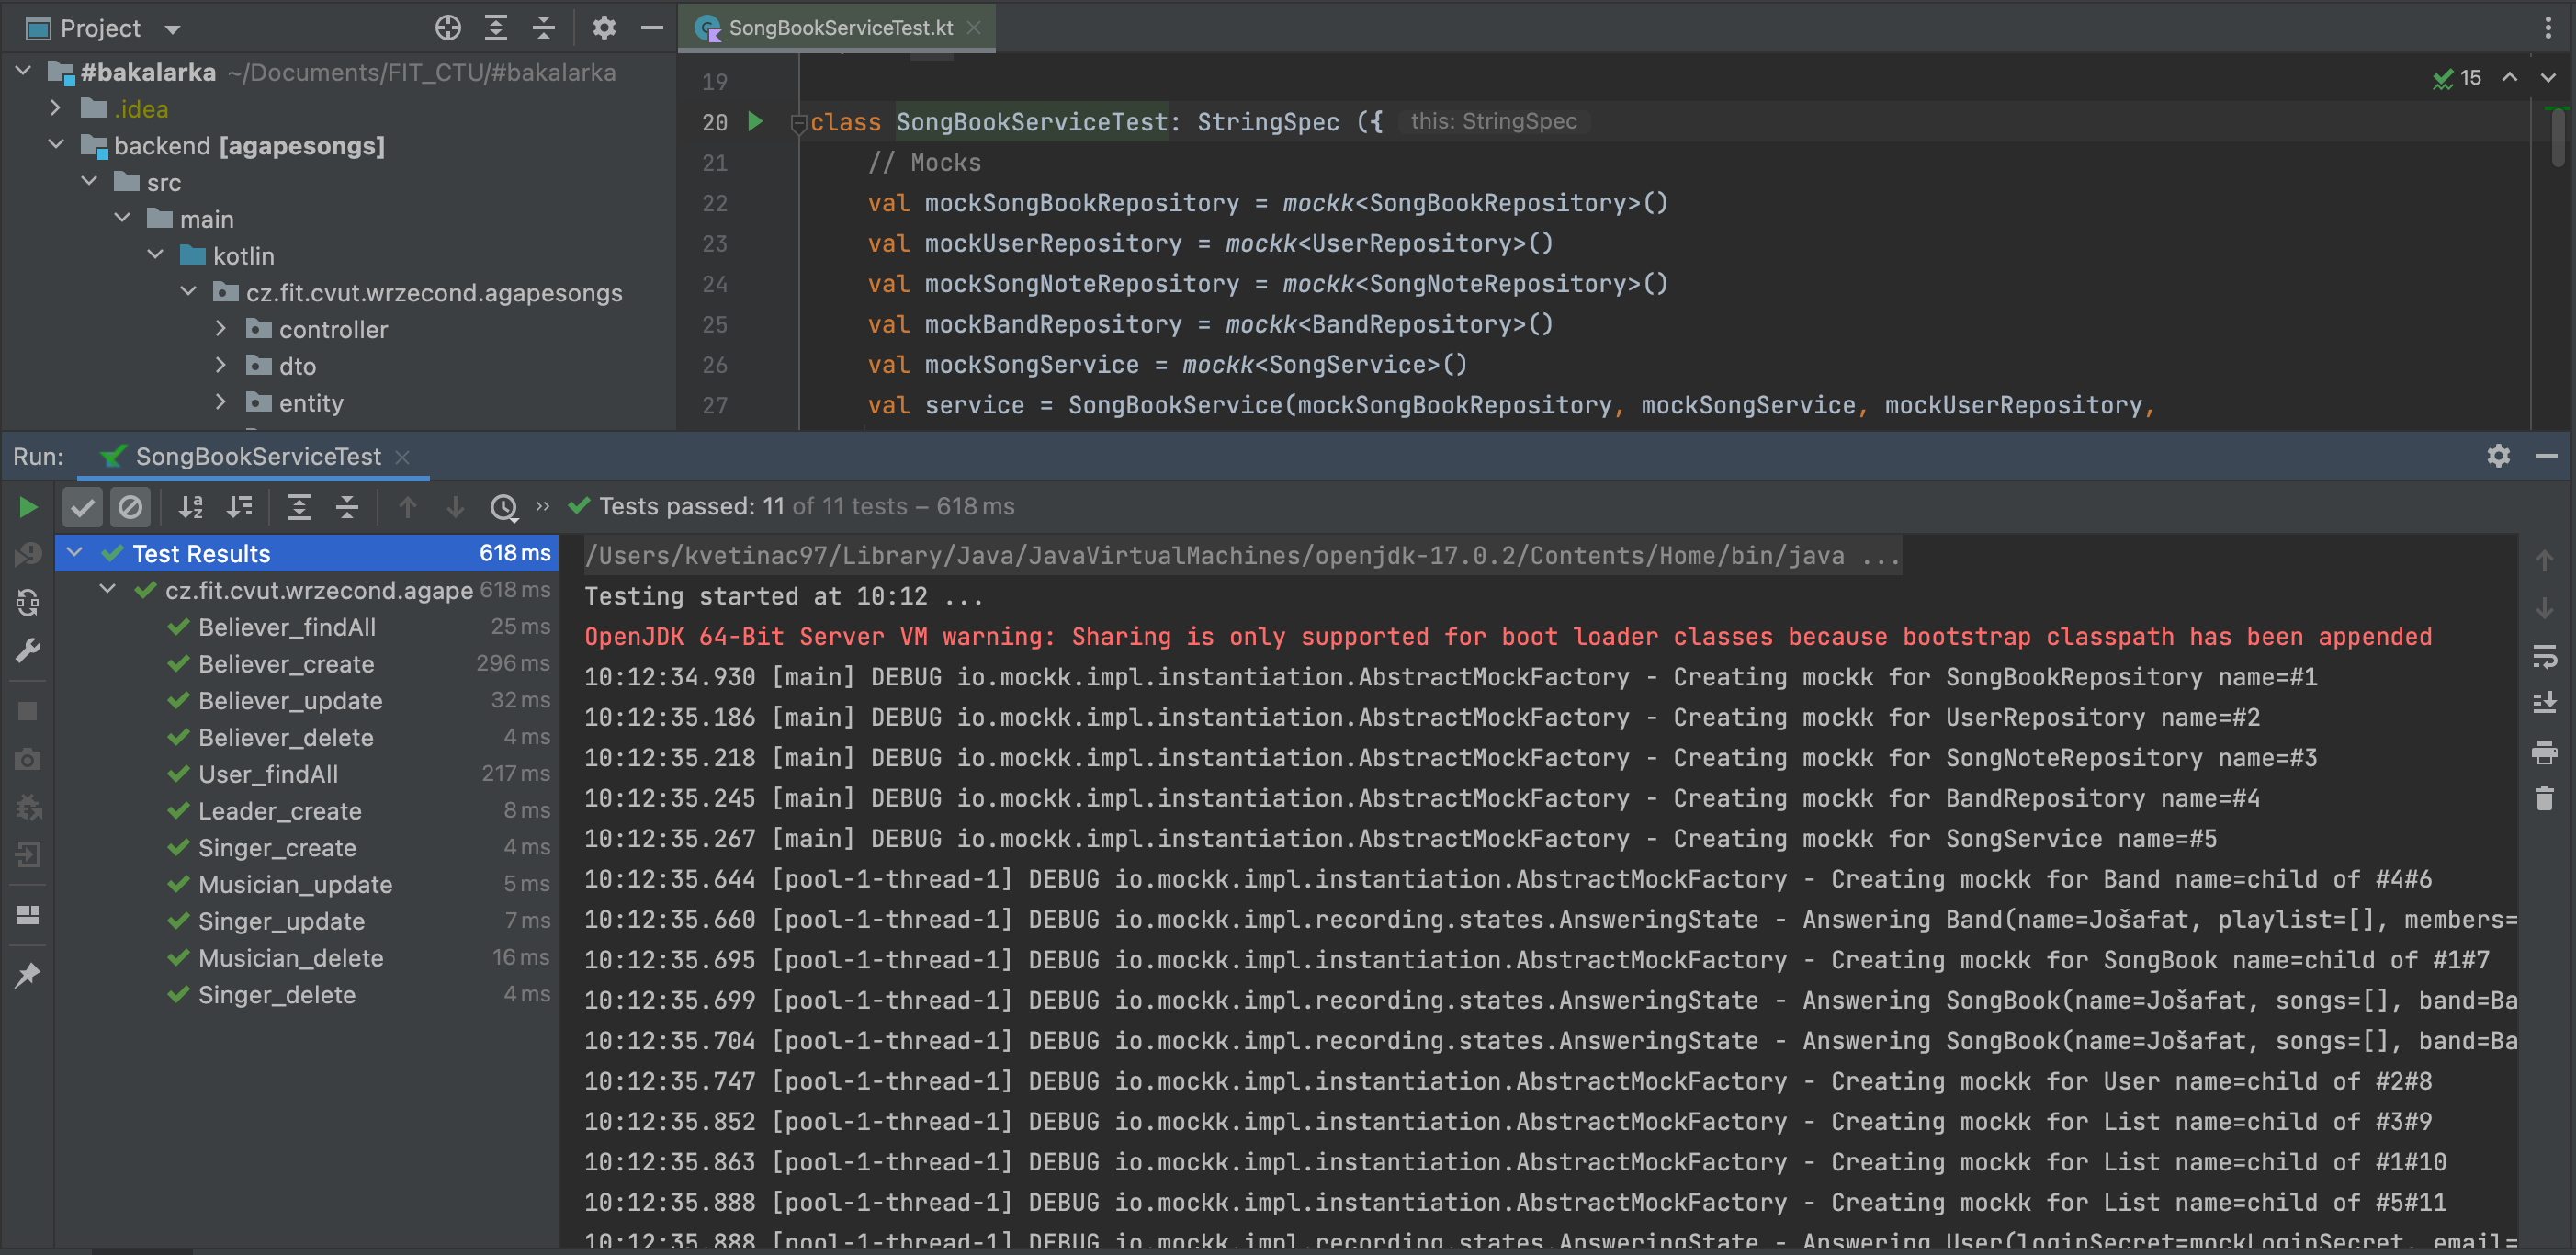
\includegraphics[width=\textwidth]{images/6-testovani/6-1-unit-test-server.png}
    \caption{Ukázka úspěšně provedených jednotkových testů serveru}
\end{figure}

\subsubsection{Aplikace}

Pro testování mobilní aplikace jsem využil nativní framework XCTest \cite{xctest}. V tomto frameworku každá třída dědí ze třídy \texttt{XCTestCase} a jednotlivé testy jsou implementovány jako její metody. Před spuštěním každého testu je zavolána metoda \texttt{setUp()}, po jeho dokončení pak metoda \texttt{tearDown()}. Pro vytváření mocků nepoužívám žádný framework -- vytvářím je ručně pomocí protocol-oriented programování. Všechny testy v aplikaci pak dědí ze třídy \texttt{AgapeSongsTestCase}, do které jsem předpřipravil dependency injection mocků a třídy \texttt{AppState}.

\begin{listing}[H]
\begin{minted}[breaklines,breaksymbolleft=]{swift}
func testLoadSongBooksEmpty() async {
    songBookService.songBookListResponse = .success([SongBookDTO]())
    await viewModel.loadSongBooks()
    
    XCTAssertTrue(songBookService.songBookListCalled)
    XCTAssertEqual(viewModel.songBooks, [SongBook]())
    XCTAssertEqual(viewModel.state, .success)
}
\end{minted}
\caption[Ukázka metody pro otestování načtení seznamu zpěvníků v aplikaci]{Ukázka metody pro otestování načtení seznamu zpěvníků. Při testování je nejprve mocku nastavena odpověď, následně se asynchronně zavolá testovaná metoda a nakonec se zkontroluje, zda byla metoda zavolána a vrátila požadovanou návratovou hodnotu}
\end{listing}

\begin{figure}[H]
    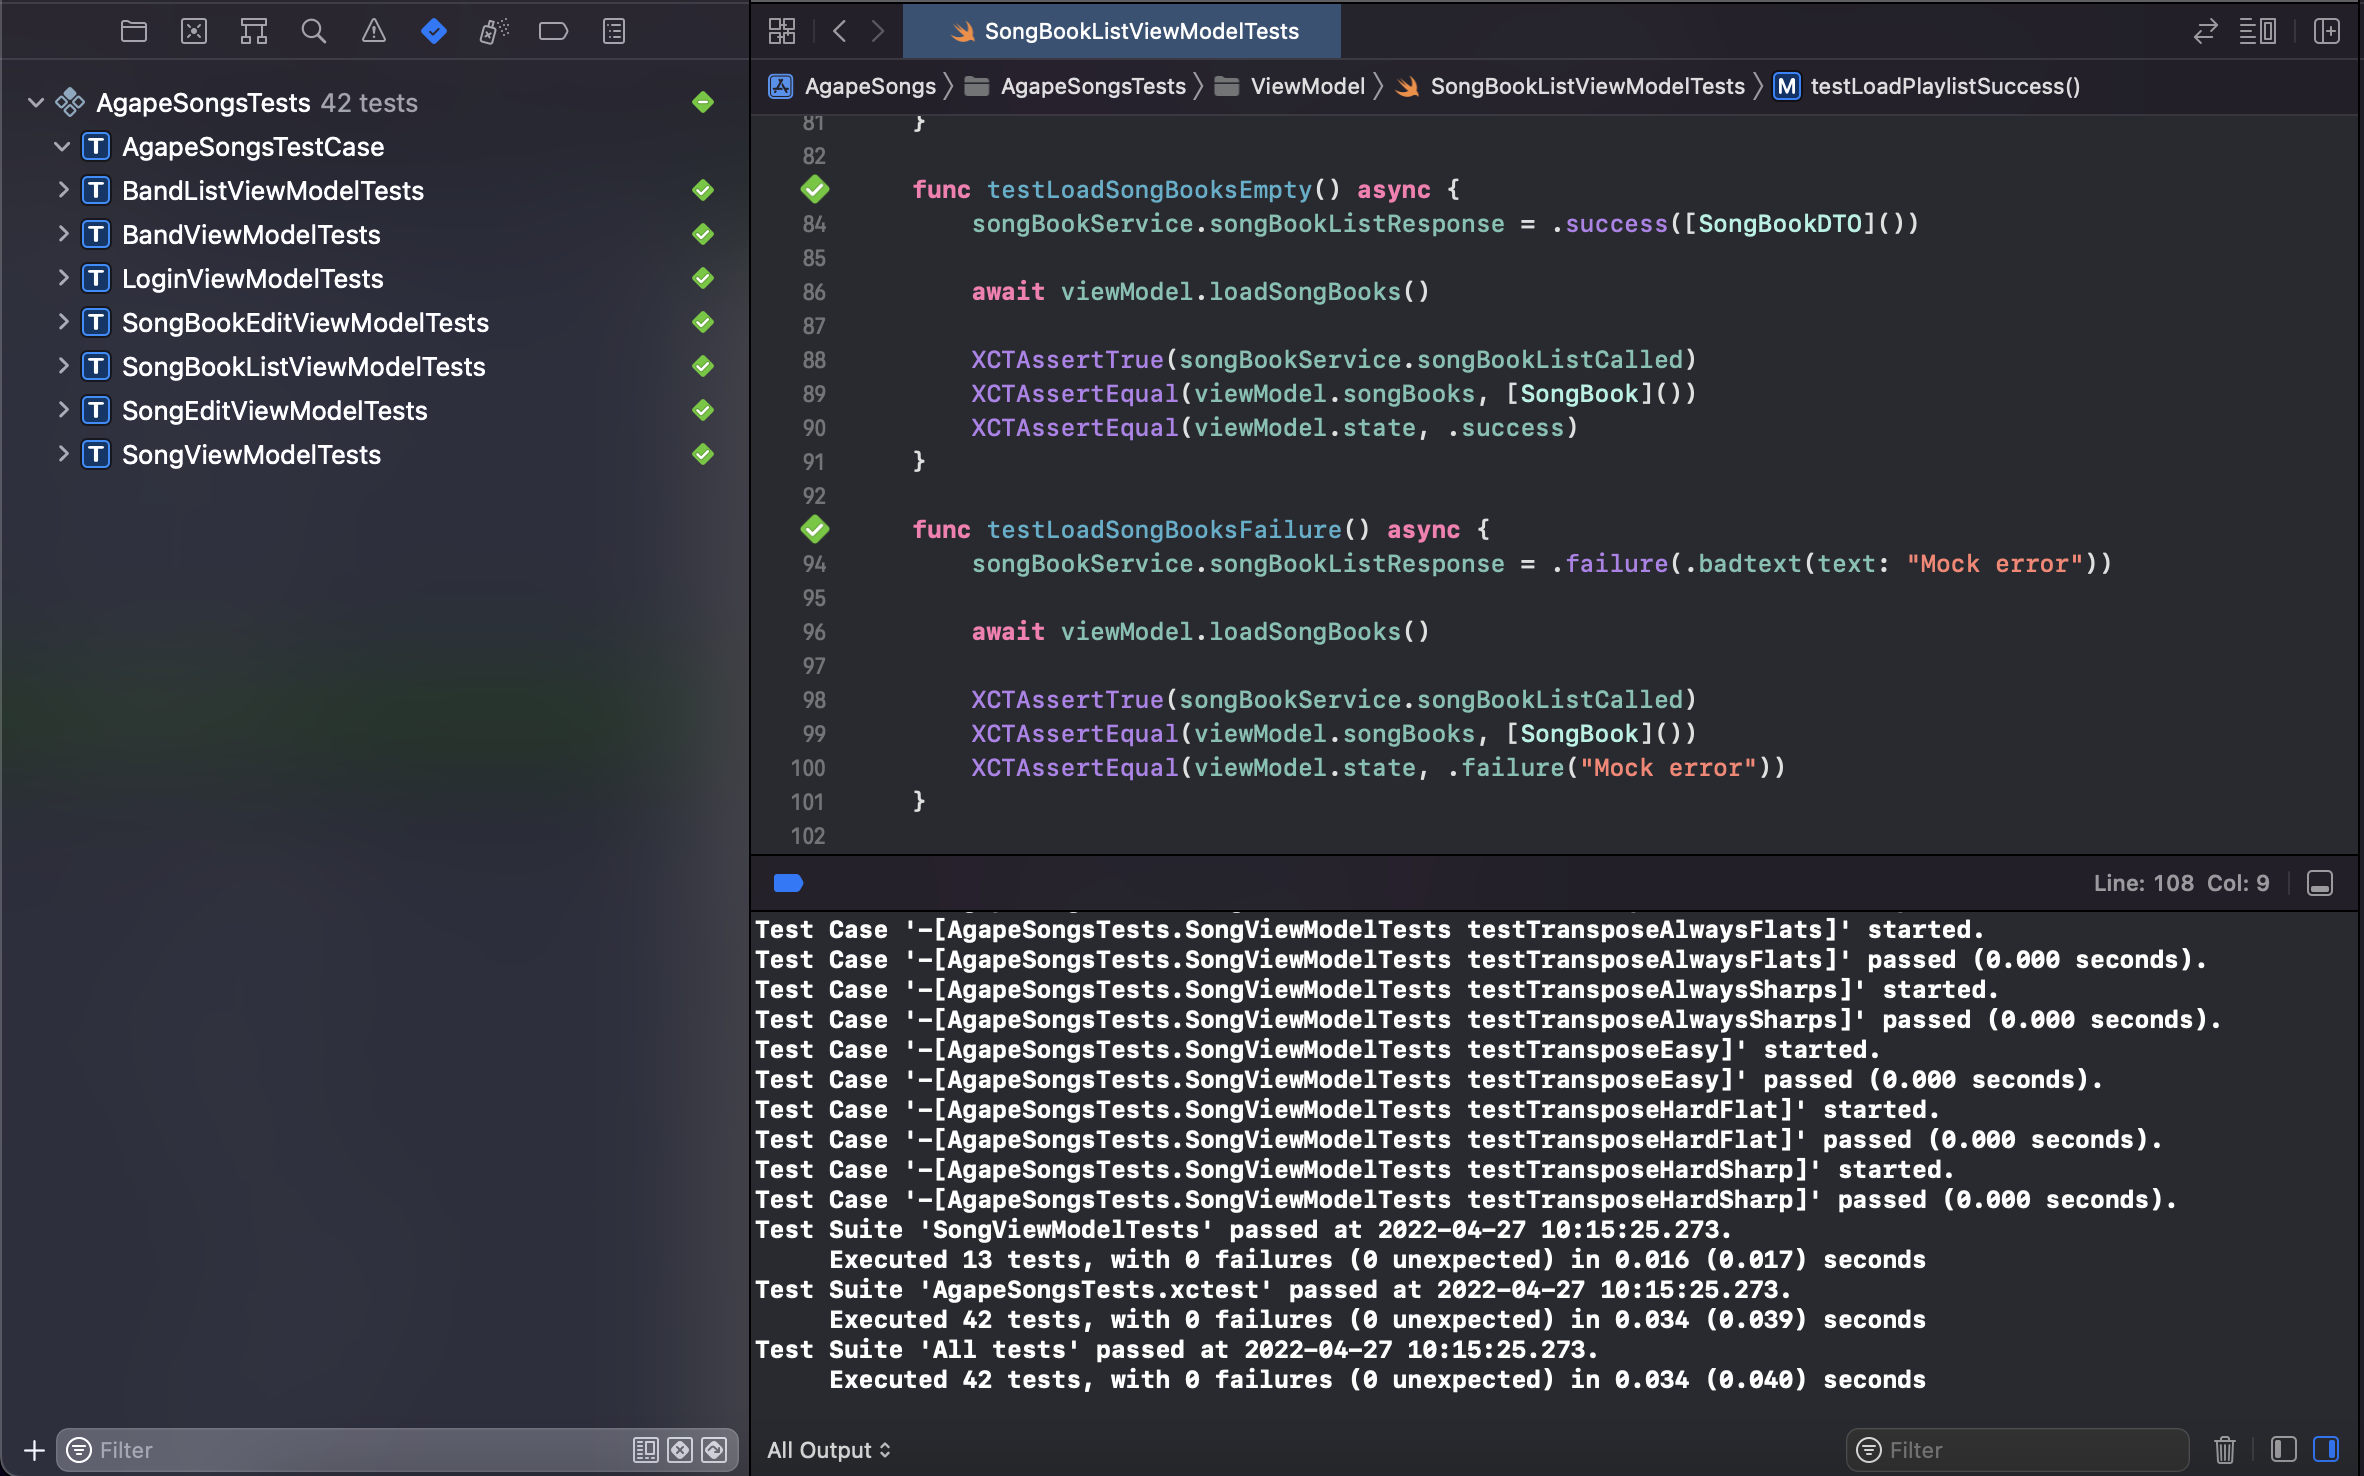
\includegraphics[width=\textwidth]{images/6-testovani/6-2-unit-test-aplikace.png}
    \caption{Ukázka úspěšně provedených jednotkových testů aplikace}
\end{figure}

\subsection{Integrační testy}

Automatizovaně testuji také vytvořené REST API, a to s pomocí programu Postman \cite{postman}. Ten umožňuje definovat jednotlivé sady požadavků a po provedení každého požadavku zavolat vlastní testy napsané v programovacím jazyce JavaScript.

\begin{listing}[H]
\begin{minted}[breaklines,breaksymbolleft=]{javascript}
pm.test("Response contains Agapebend first", function () {
    pm.expect(pm.response.json()[0].name).to.eql("Agapebend")
});
\end{minted}
\caption[Ukázka integračních testů v programu Postman]{Ukázka testu pro endpoint /songbook (zpěvníky), který zkontroluje, že odpověď na~požadavek je JSON pole, které obsahuje jeden zpěvník, jehož jméno je Agapebend}
\end{listing}

\begin{figure}[H]
    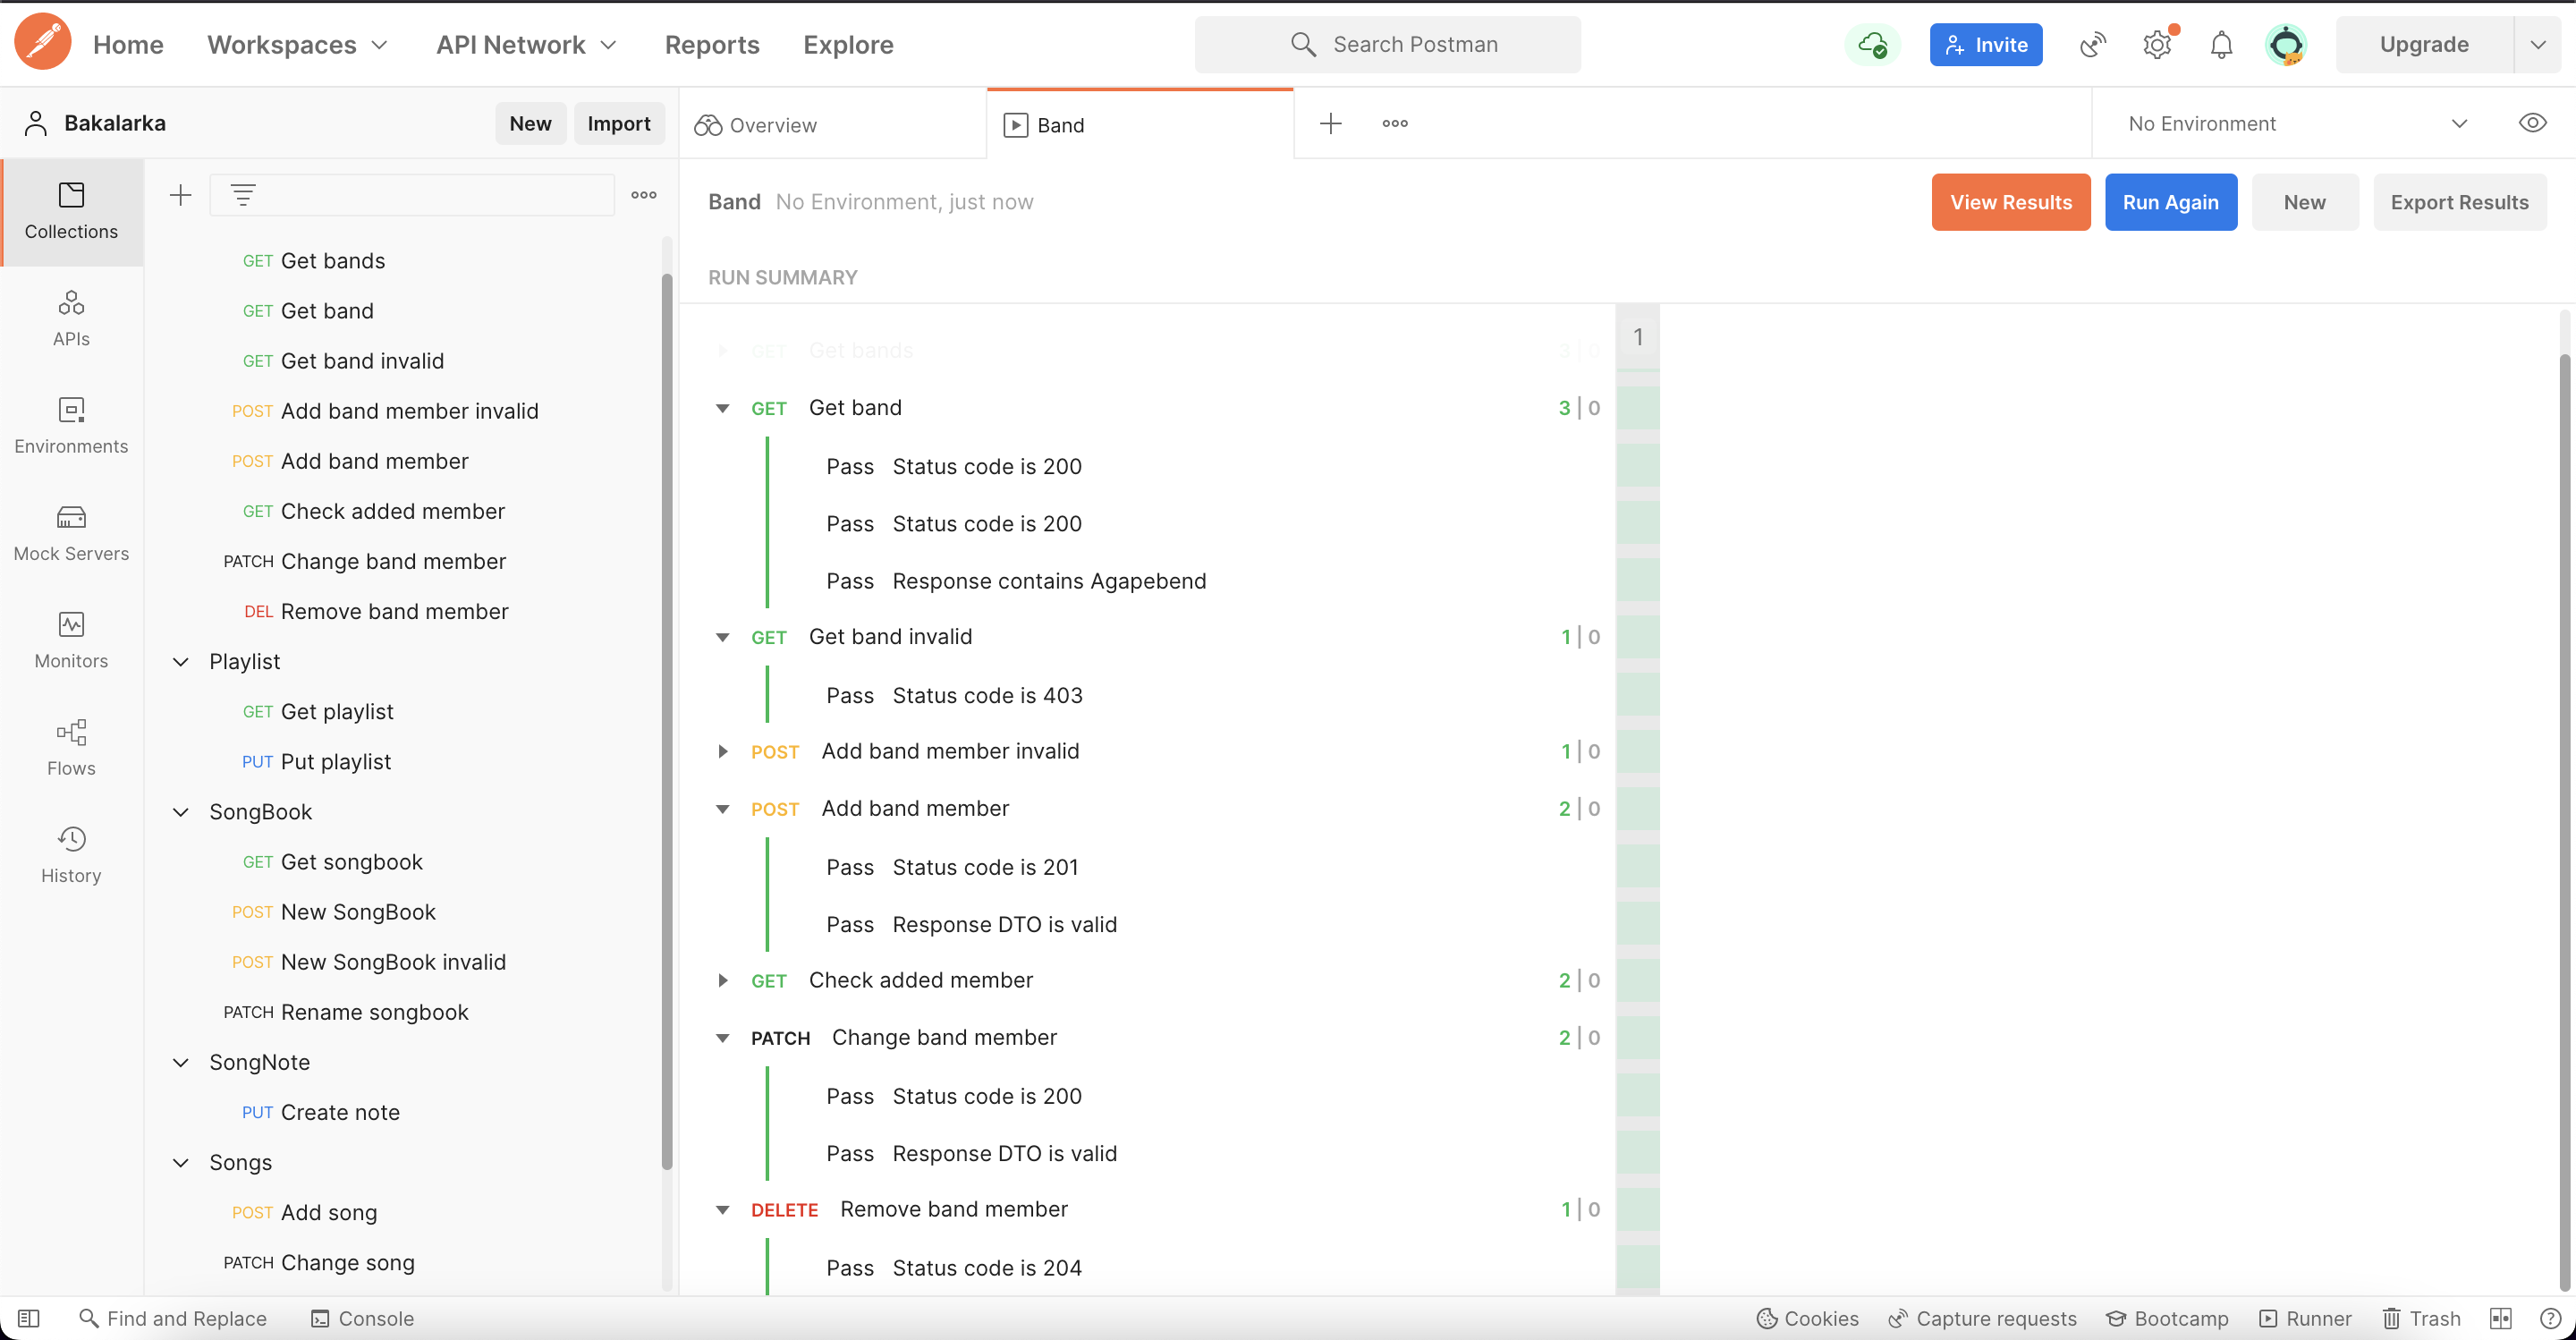
\includegraphics[width=\textwidth]{images/6-testovani/6-3-integracni-test-postman.png}
    \caption{Ukázka úspěšně provedených integračních testů pro endpoint /band}
\end{figure}

\subsection{Přínos}

Díky jednotkovým testům jsem byl schopen v serveru nebo v aplikaci chybu odhalit ještě dříve, než jsem je předal uživatelům k testování. Jednalo se například o chybu na serveru, kdy u písně, která již měla nastavené číslo v rámci zpěvníku nešlo toto číslo odstranit nebo chybu, kdy se při změně písně na začátek textu vždy přidal nový řádek. V aplikaci jsem pomocí jednotkových testů odhalil chyby v logice pro zalamování a chybu, kdy jsem zapomněl přidat možnost tóniny A dur. S pomocí integračních testů API v programu Postman jsem odhalil chybu, kdy API poskytovalo seznam zpěvníků ve špatném pořadí.

\section{Uživatelské testy}

Uživatelské testy provádí přímo budoucí uživatelé systému. V průběhu uživatelských testů lze pozorovat způsob, jakým uživatelé systém používají a často odhalí chyby, na které programátoři v průběhu automatizovaných testů nepřišli. Dalším velkým přínosem uživatelských testů je pak také zpětná vazba na aktuální verzi aplikace.

\subsection{TestFlight}

Pro to, aby mohli uživatelé aplikaci testovat, je třeba, aby si aplikaci nainstalovali. Na Apple zařízení lze aplikaci oficiálně nainstalovat pouze ze dvou zdrojů -- oficiálního obchodu App Store \cite{app-store} a testovací platformy TestFlight \cite{testflight}. Zveřejnění v oficiálním obchodě ale není vhodnou metodou pro distribuci aplikace za účelem testování, protože takto zveřejněná aplikace je viditelná pro všechny uživatele iOS a macOS zařízení, což prozatím není žádoucí.

Testovací platforma TestFlight umožňuje přehlednou a jednoduchou správu a distribuci testovacích verzí aplikace. Nové verze se do ní nahrávají přímo z programovacího prostředí Xcode. Nahrané verze lze pak spravovat v prostředí App Store Connect \cite{app-store-connect}, odkud je lze distribuovat mezi dvě skupiny uživatelů -- interní a externí. Výhodou interního testování je možnost okamžité distribuce, nevýhodou je ale nutnost uživatele přidat přímo jako členy organizace FIT ČVUT, což z technických důvodů v mém případě není možné.

\begin{figure}[H]
    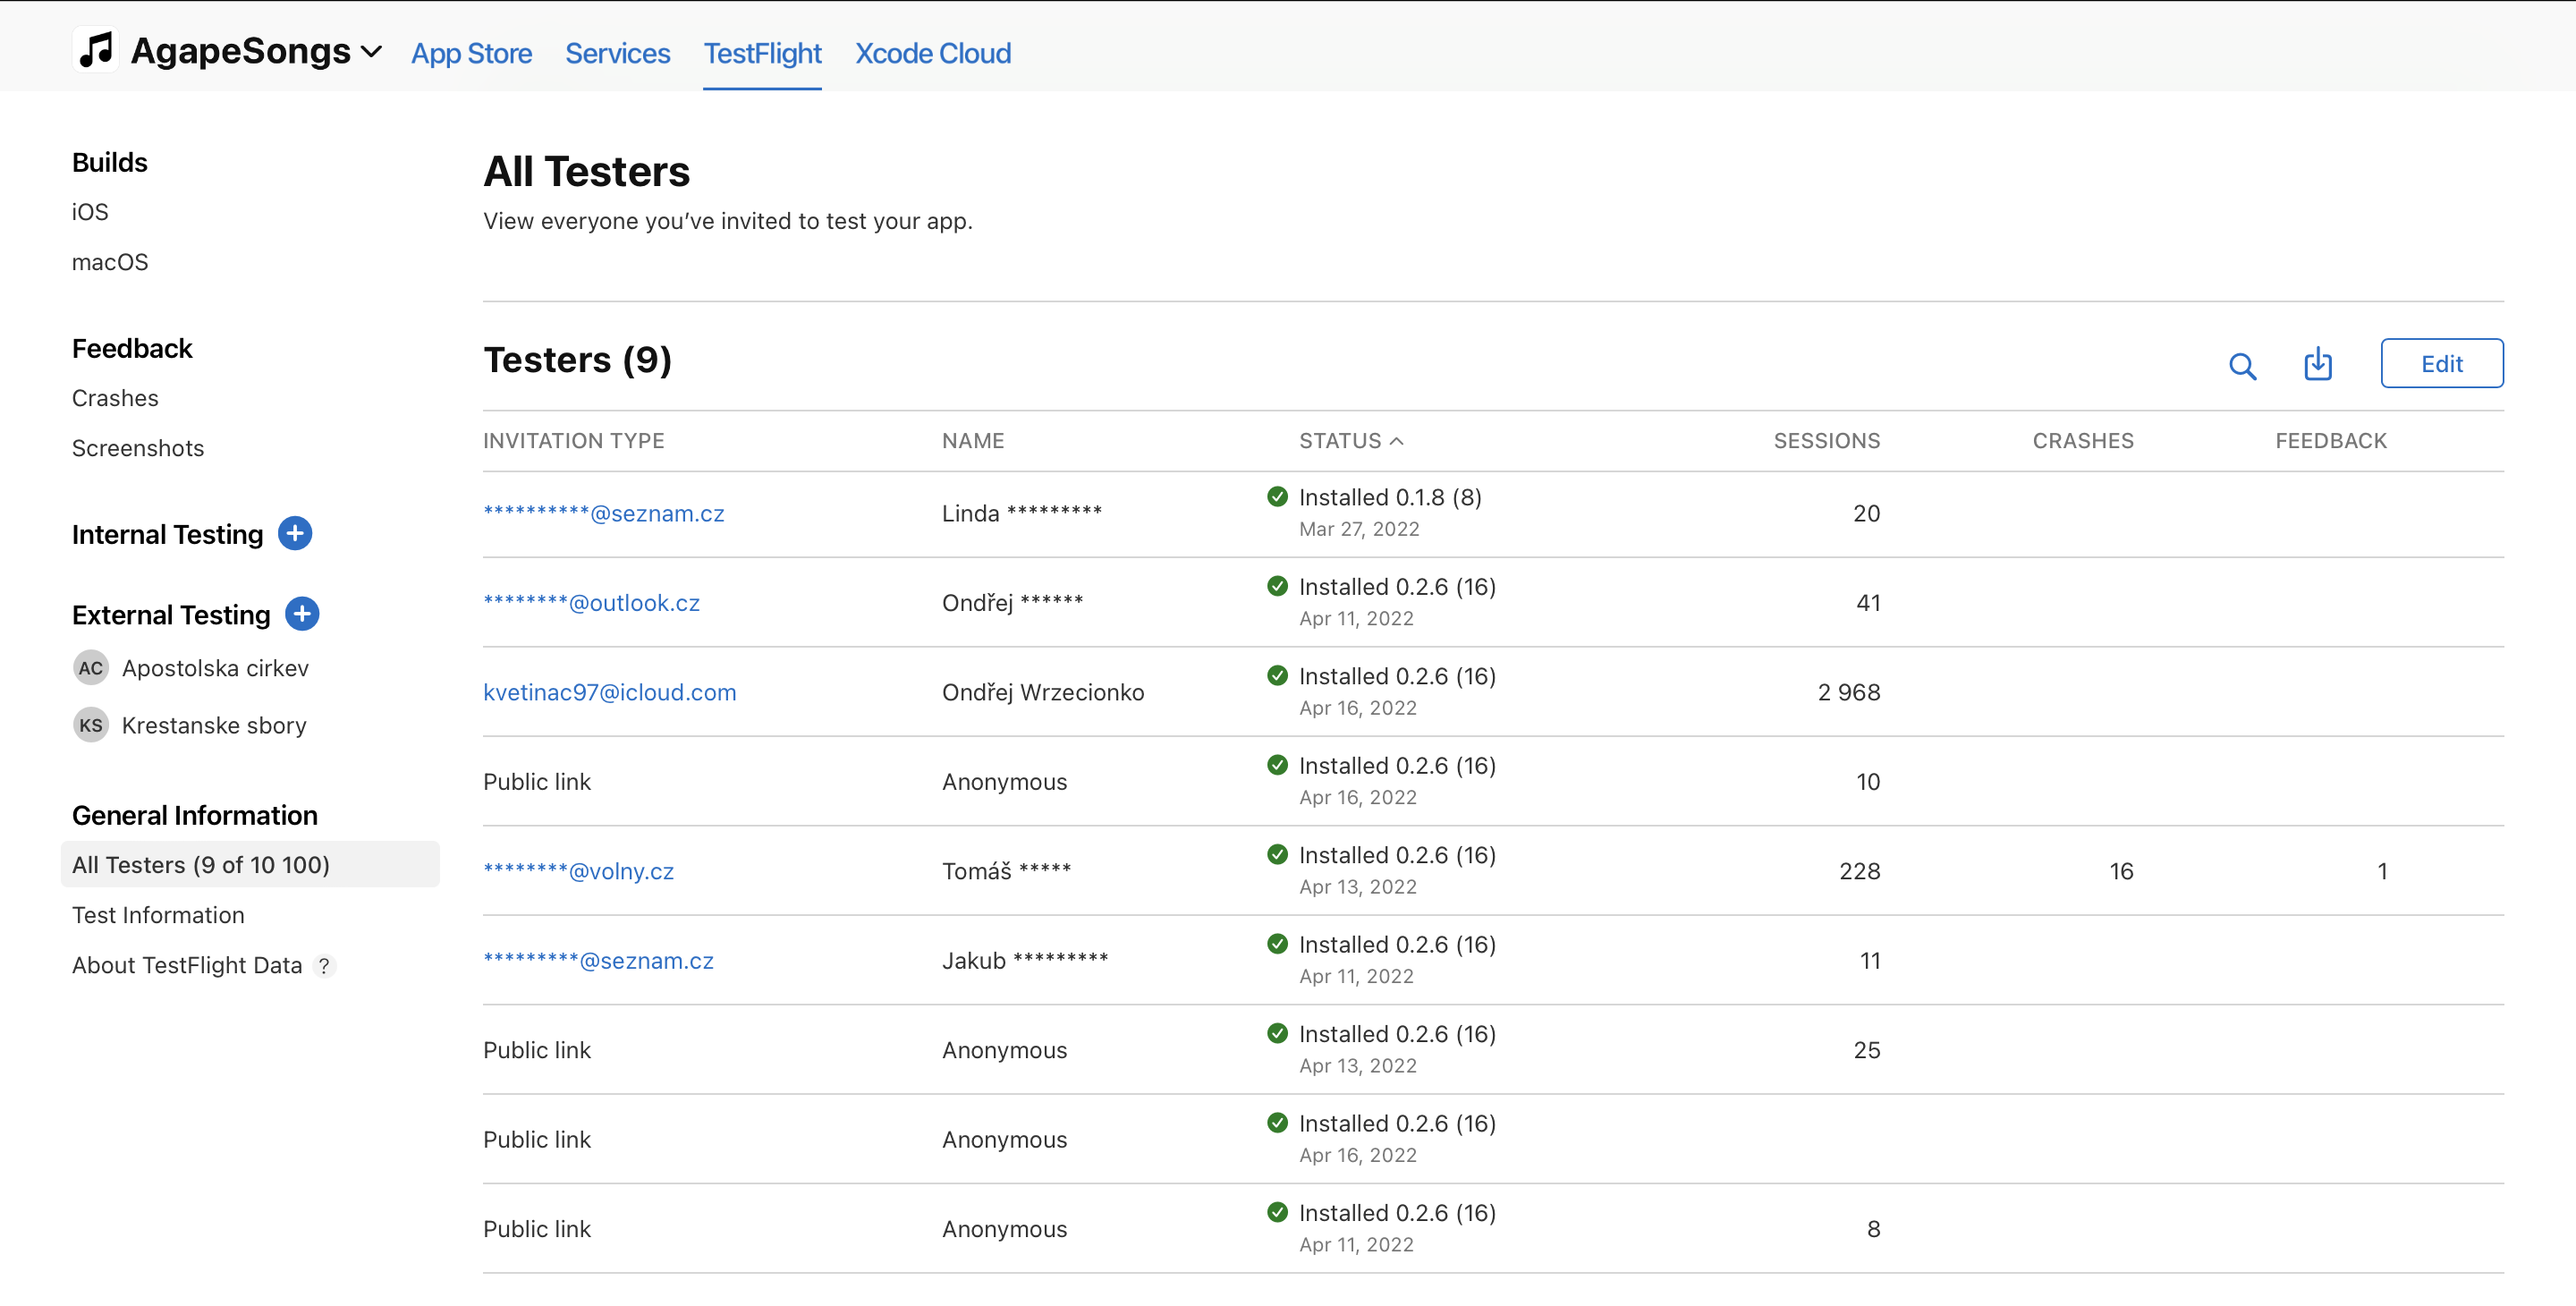
\includegraphics[width=\textwidth]{images/6-testovani/6-4-testflight-uzivatele.png}
    \caption{Ukázka správy testujících uživatelů v testovací platformě TestFlight}
\end{figure}

K externímu testování lze pozvat libovolného uživatele s Apple zařízením, nevýhodou je ale potřeba schválení každé nové verze ve zrychleném procesu App Review, který v praxi trvá přibližně 1 až 2 pracovní dny. Pro testování aplikace jsem si tedy vybral externí testování v rámci platformy TestFlight.

\begin{figure}[H]
    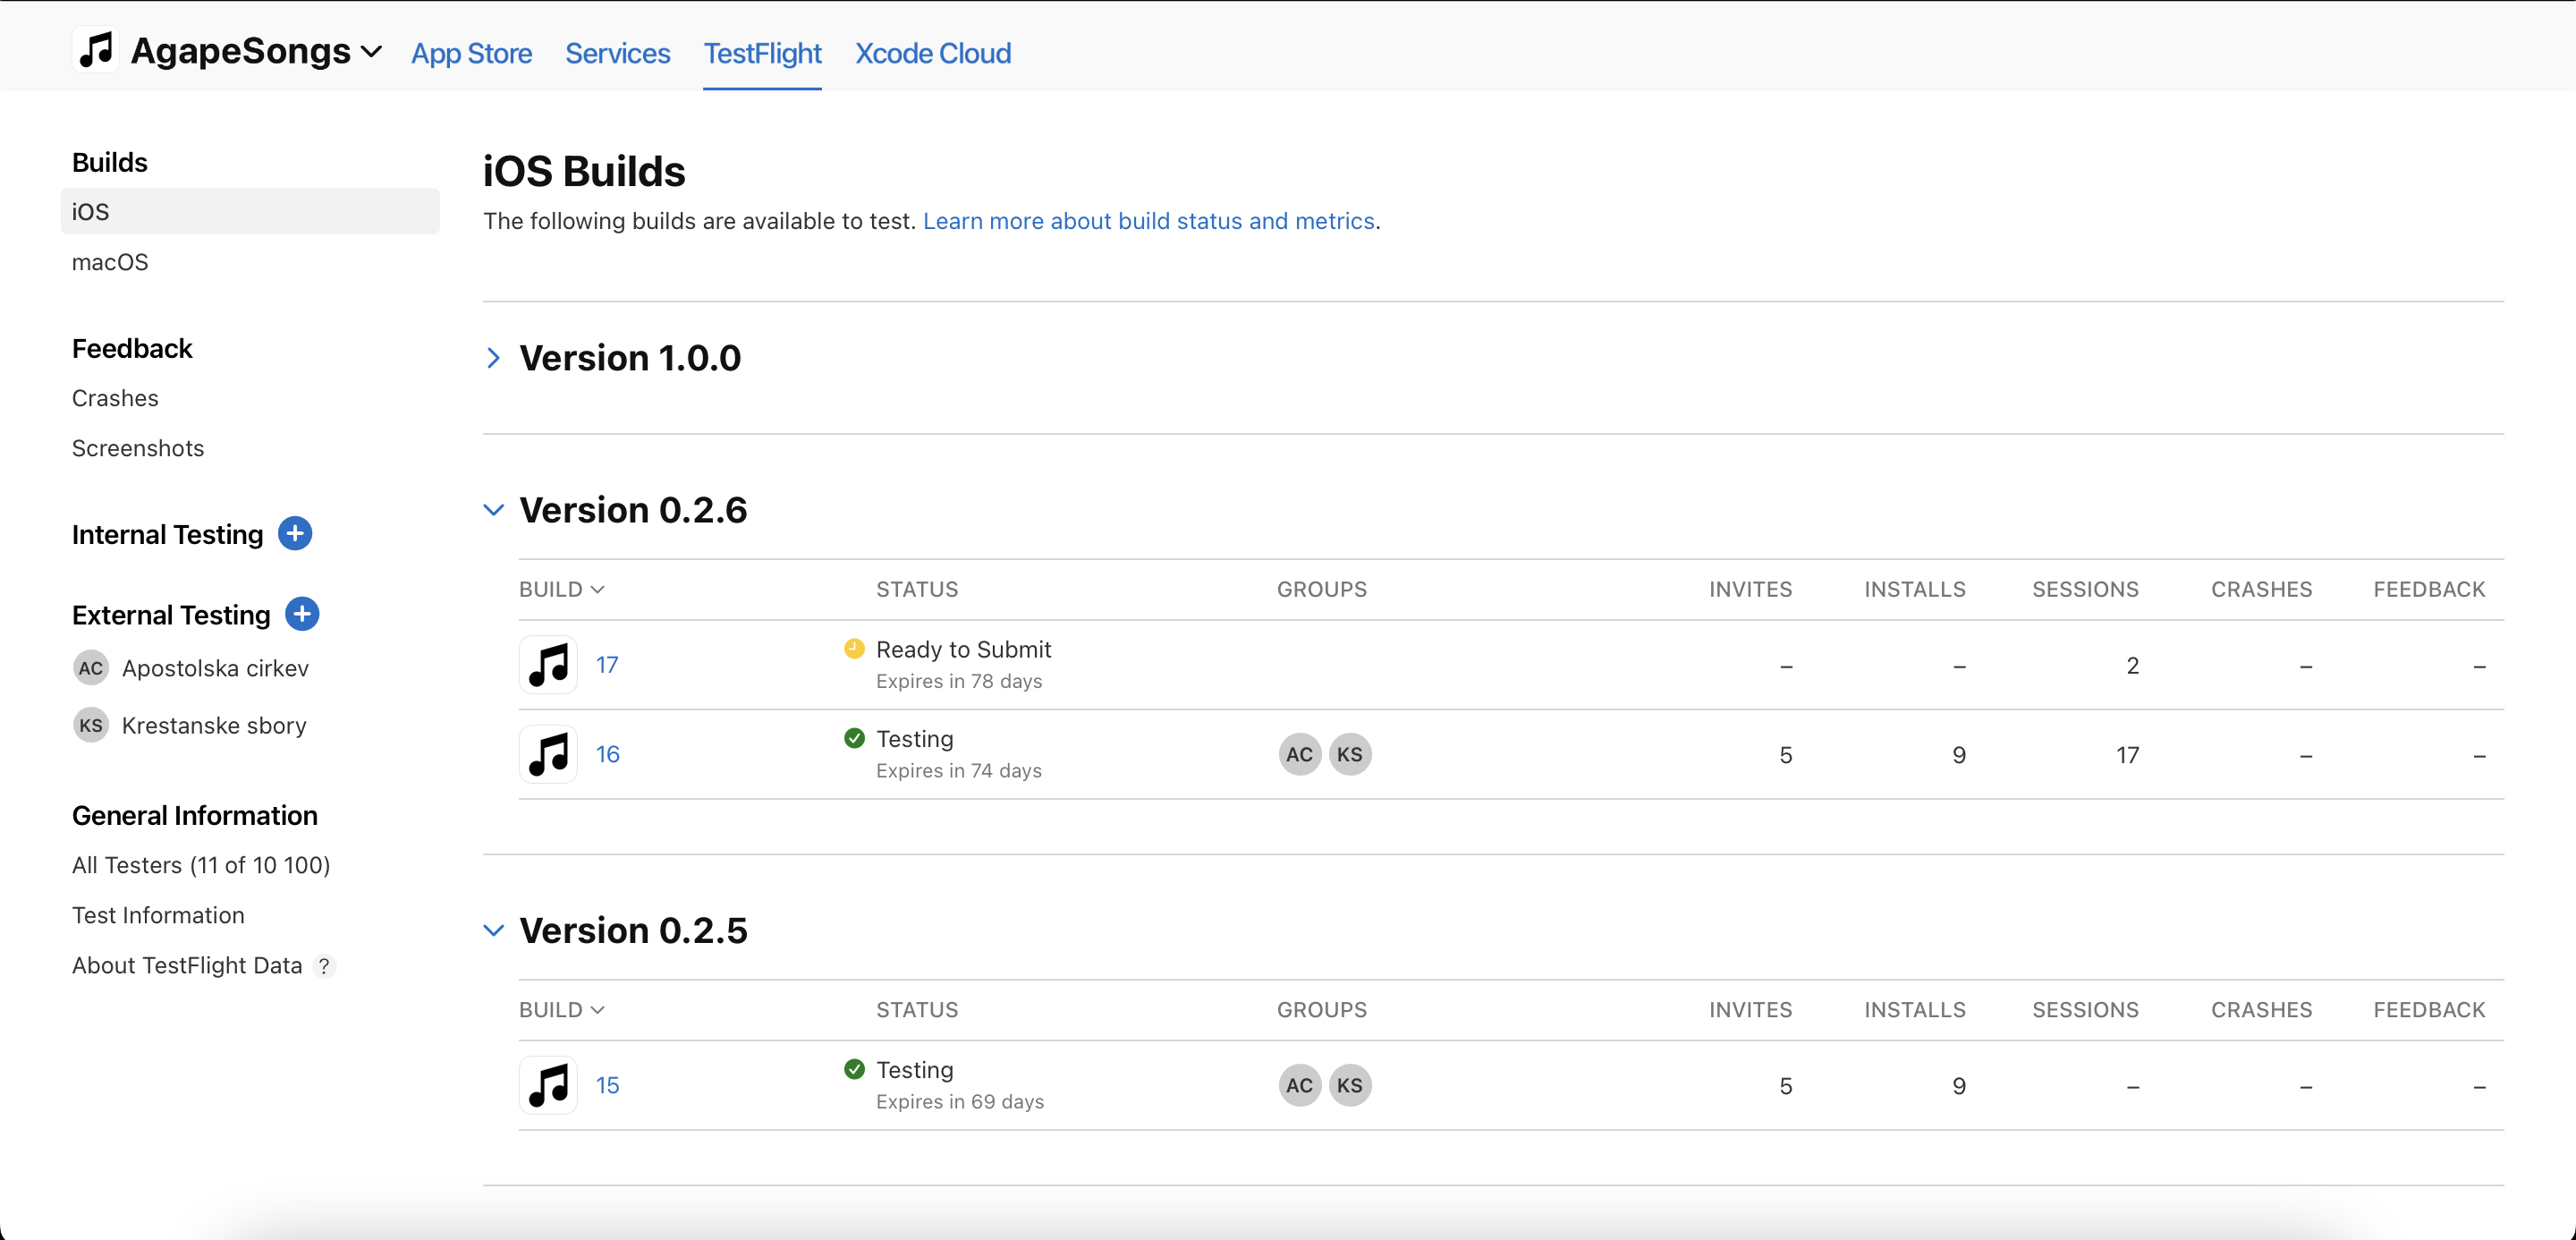
\includegraphics[width=\textwidth]{images/6-testovani/6-5-testflight-verze.png}
    \caption{Ukázka správy verzí aplikace v testovací platformě TestFlight}
\end{figure}

\subsection{AC Agapé}

Nejdéle jsem aplikaci testoval ve spolupráci s jednou z kapel v AC Agapé. Jak jsem psal v~analýze, v~AC Agapé jsou dvě kapely, které se střídají. Věděl jsem tedy, že tato kapela bude zkoušet 26. 3. 2022, 9. 4. 2022 a 23. 4. 2022, snažil jsem se tedy naplánovat tvorbu aplikace tak, abych byl schopen na první ze zmíněných sobot dodat použitelnou verzi aplikace.

\subsubsection{První zkouška}

Ve středu 23. 3. 2022 jsem do TestFlightu odeslal první verzi aplikace, ve čtvrtek 24. 3. 2022 byla schválena a odeslal jsem ji do kapely k testování. Vedoucí kapely mi ale vzápětí odpověděl, že členům kapely aplikace nejde nainstalovat. Po pár minutách zkoumání jsme zjistili, že jsem aplikaci omylem nastavil minimální verzi podporovaného operačního systému jako iOS 15.4, respektive macOS 12.1, zatímco členové kapely mají na zařízeních starší verze. Okamžitě jsem tedy v aplikaci snížil minimální verzi na iOS 15.0 a macOS 12.0 a odeslal jí znova ke schválení. Apple jí ale schválil až v půlnoci ze soboty na neděli a první zkoušku jsem tedy promeškal. Ponaučil jsem se ale a věděl jsem tak, že další verzi musím členům kapely odeslat s minimálně týdenním předstihem.

\subsubsection{Druhá zkouška}

Verzi aplikace pro druhou zkoušku (v sobotu 9. 4. 2022) jsem nahrál do TestFlightu pro jistotu už 31. 3. 2022, tedy s více než týdenním předstihem. 1. 4. 2022 mi byla verze zamítnuta, jelikož obsahovala chráněný autorský obsah -- písně ve zpěvnících. Musel jsem tedy upravit server tak, aby nově registrovaným uživatelům zobrazil pouze ukázkový zpěvník s ukázkovou písní a skutečné písně zůstaly viditelné pouze pro stávající uživatele. Po této úpravě jsem aplikaci znovu odeslal ke~schválení a 3. 4. 2022 byla aplikace schválena. V průběhu týdne jsem pak ještě doimplementoval funkci transpozice akordů.

Na sobotní zkoušce kapely jsem pak byl přítomen jako pozorovatel a po zkoušce jsem s členy kapely diskutoval o tom, jak se jim aplikace používala. Hodně členů kapely si stěžovalo na malou velikost písma názvu písní v seznamu. Vedoucímu chybělo v názvu číslo písně ve zpěvníku, které sděloval členům kapely s papírovým zpěvníkem. Zásadnější chybou bylo pak nesprávné přizpůsobení aplikace světlému módu. Aplikace jsem totiž vyvíjel v tmavém módu s použitím bílé barvy textu, která na bílém pozadí nebyla vidět. Někteří členové kapely tak museli dočasně přepnout aplikaci do tmavého módu. Při používání transpozice si pak někteří členové stěžovali na formát akordů -- některým vadil formát s křížky, některým s béčky.

Na základě této zkoušky jsem k názvu písně v seznamu přidal její číslo a aplikaci jsem otestoval také ve světlém módu, přičemž jsem našel více míst, kde se zobrazoval bílý text na~bílém pozadí. Stížnosti ohledně velikosti písma a formátu akordů jsem vyřešil přidáním nové obrazovky Nastavení aplikace, ve které si může uživatel nastavit velikost textu v seznamech a preferovaný formát zobrazení akordů.

\begin{figure}
    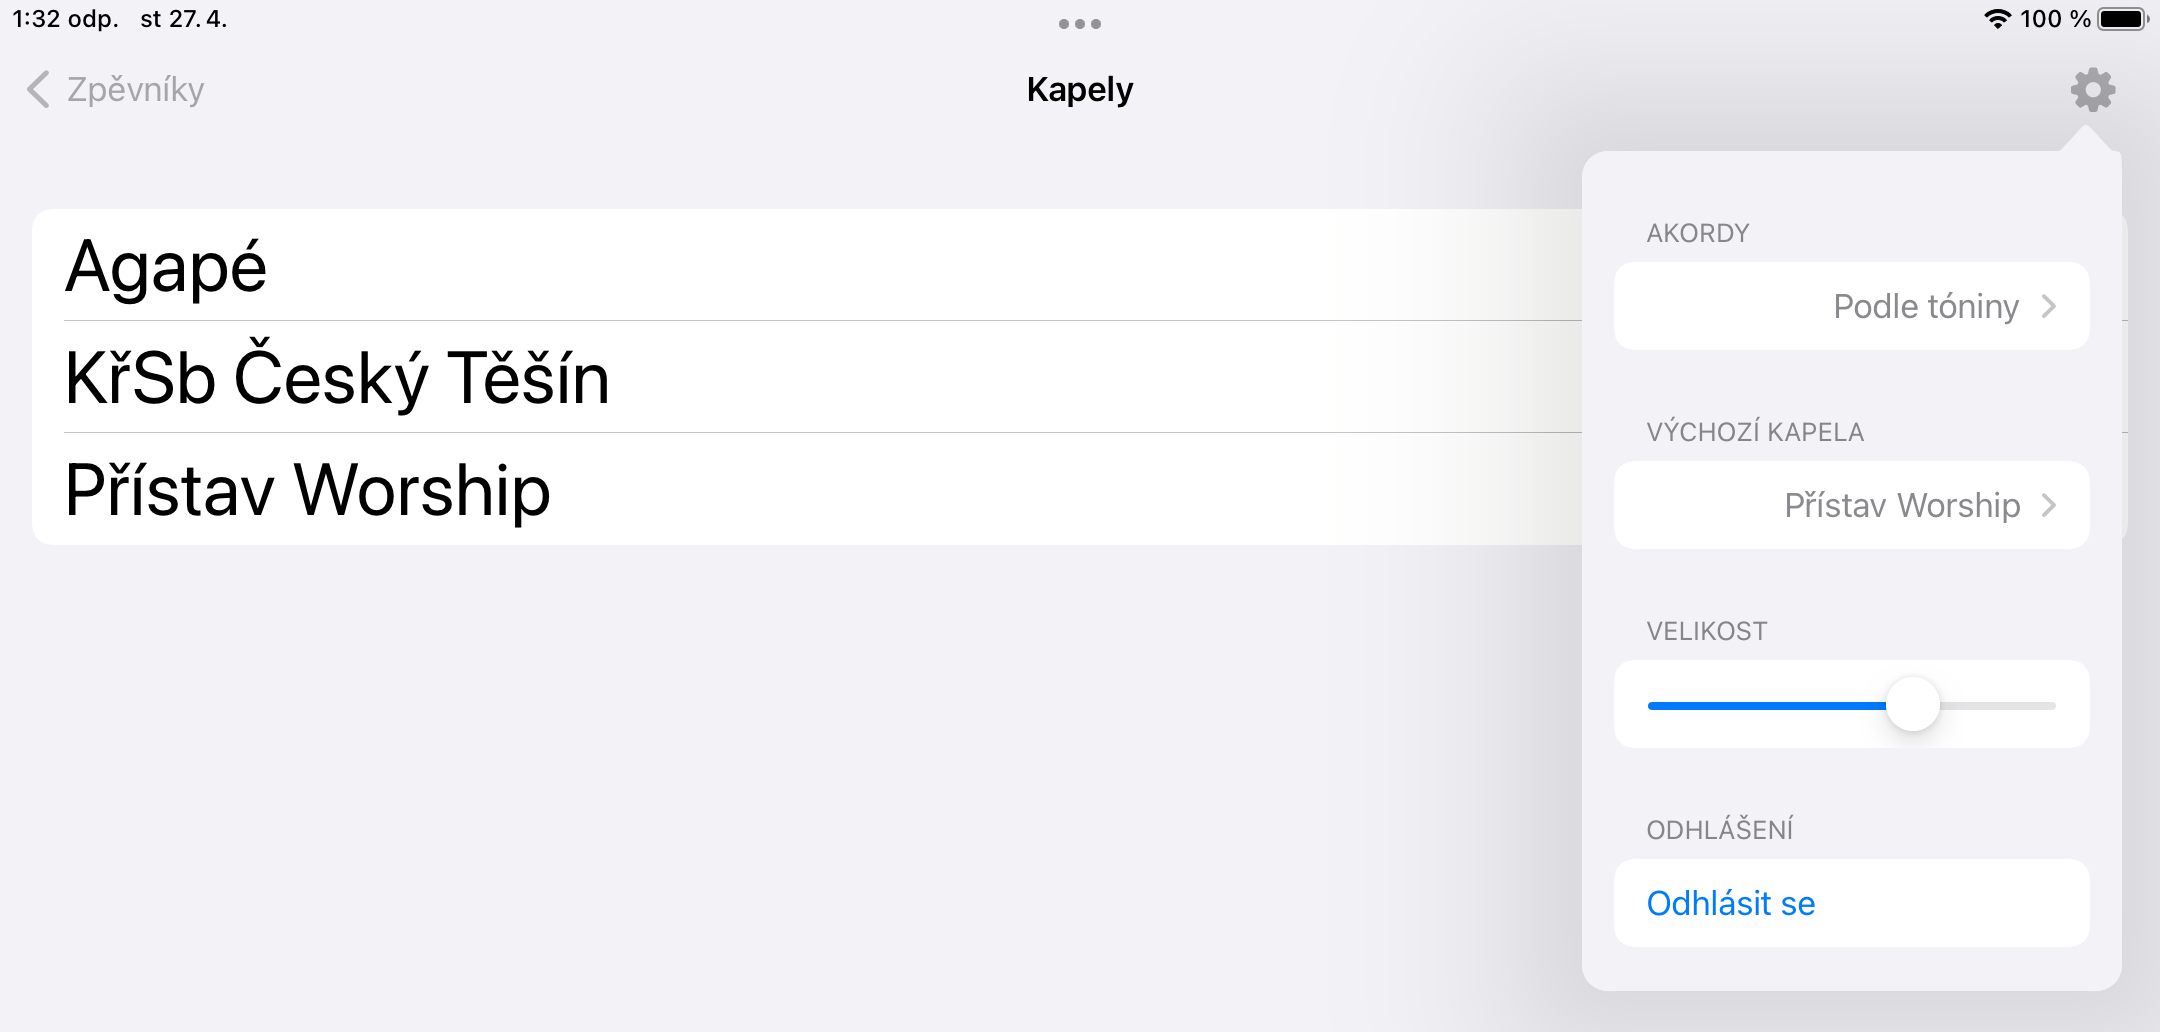
\includegraphics[width=\textwidth]{images/6-testovani/6-6-nastaveni-ipad.png}
    \caption[Ukázka obrazovky Nastavení aplikace na iOS]{Ukázka obrazovky pro nastavení velikosti písma, preferovaného formátu akordů a výchozí kapely pro nahrávání playlistu}
\end{figure}

\subsubsection{Třetí zkouška}

Třetí zkouška se konala v sobotu 23. 4. 2022. Po této zkoušce jsem dostal od členů kapely na~aplikaci již pouze pozitivní zpětnou vazbu spolu s návrhy na další vylepšení aplikace. Tyto návrhy podrobněji popíšu v kapitole \nameref{zaver}.

\subsection{Přístav Worship}

Další kapelou, ve které jsem testoval aplikaci, byla kapela Přístav Worship, která je součástí KřSb Český Těšín. Narozdíl od ostatních kapel je tato kapela složena převážně z mladých hudebníků, kteří všichni vlastní mobilní telefon s operačním systémem iOS. V rámci zkoušky Přístav Worship, která se konala v sobotu 16. 4. 2022, jsem tak měl možnost vyzkoušet také synchronizaci playlistů mezi více zařízeními v průběhu zkoušky.

Při zkoušce kapela našla dvě chyby -- první chybou byla nefunkční úprava písní, které jsou v~playlistu (po upravení písně v playlistu se text písně změnil až po jejím odebrání a znovupřidání do playlistu), což bylo v průběhu zkoušky zdržující a nepříjemné. Druhou, závažnější chybou pak byla situace, kdy se po nahrání a stažení v playlistu seřadily písně podle jejich unikátního identifikátoru a ne podle původního pořadí, což způsobilo mezi členy kapely zmatek.

Na základě této zkoušky jsem tedy zprovoznil úpravu písní v playlistu a také jsem opravil funkci pro nahrání a stahování playlistu na serveru tak, aby již neprováděla řazení playlistu podle unikátního identifikátoru.

\subsection{KřSb Pyšely}

Poslední kapelou, ve které jsem testoval aplikaci, byla kapela křesťanského sboru v Pyšelích, jejíž zkoušky jsem se účastnil o víkendu 23. - 24. dubna 2022. Zdejší kapela se skládá z tří hudebníků -- kytaristy a zpěvačky, kteří použili aplikaci na iPadu a klávesisty, který používal aplikaci na Macu. Kytarista a zpěvačka byli z aplikace nadšení a pouze předali návrhy dalších možných rozšíření aplikace. Klávesista při používání aplikaci našel chyby, které byly specifické pro používání aplikace na operačním systému macOS.

První chybou byla obtížnost používání aplikace spolu se softwarem MainStage, který klávesis\-té běžně používají pro hraní na klávesy. V průběhu hraní písně klávesista v této aplikaci, která se zobrazuje na celou obrazovku a nelze změnit její velikost, potřebuje přepínat rejstříky, zatímco se dívá na akordy v aplikaci. Aplikace by tedy v operačním systému macOS měla mít možnost zobrazení jako plovoucí okno.

\begin{figure}
    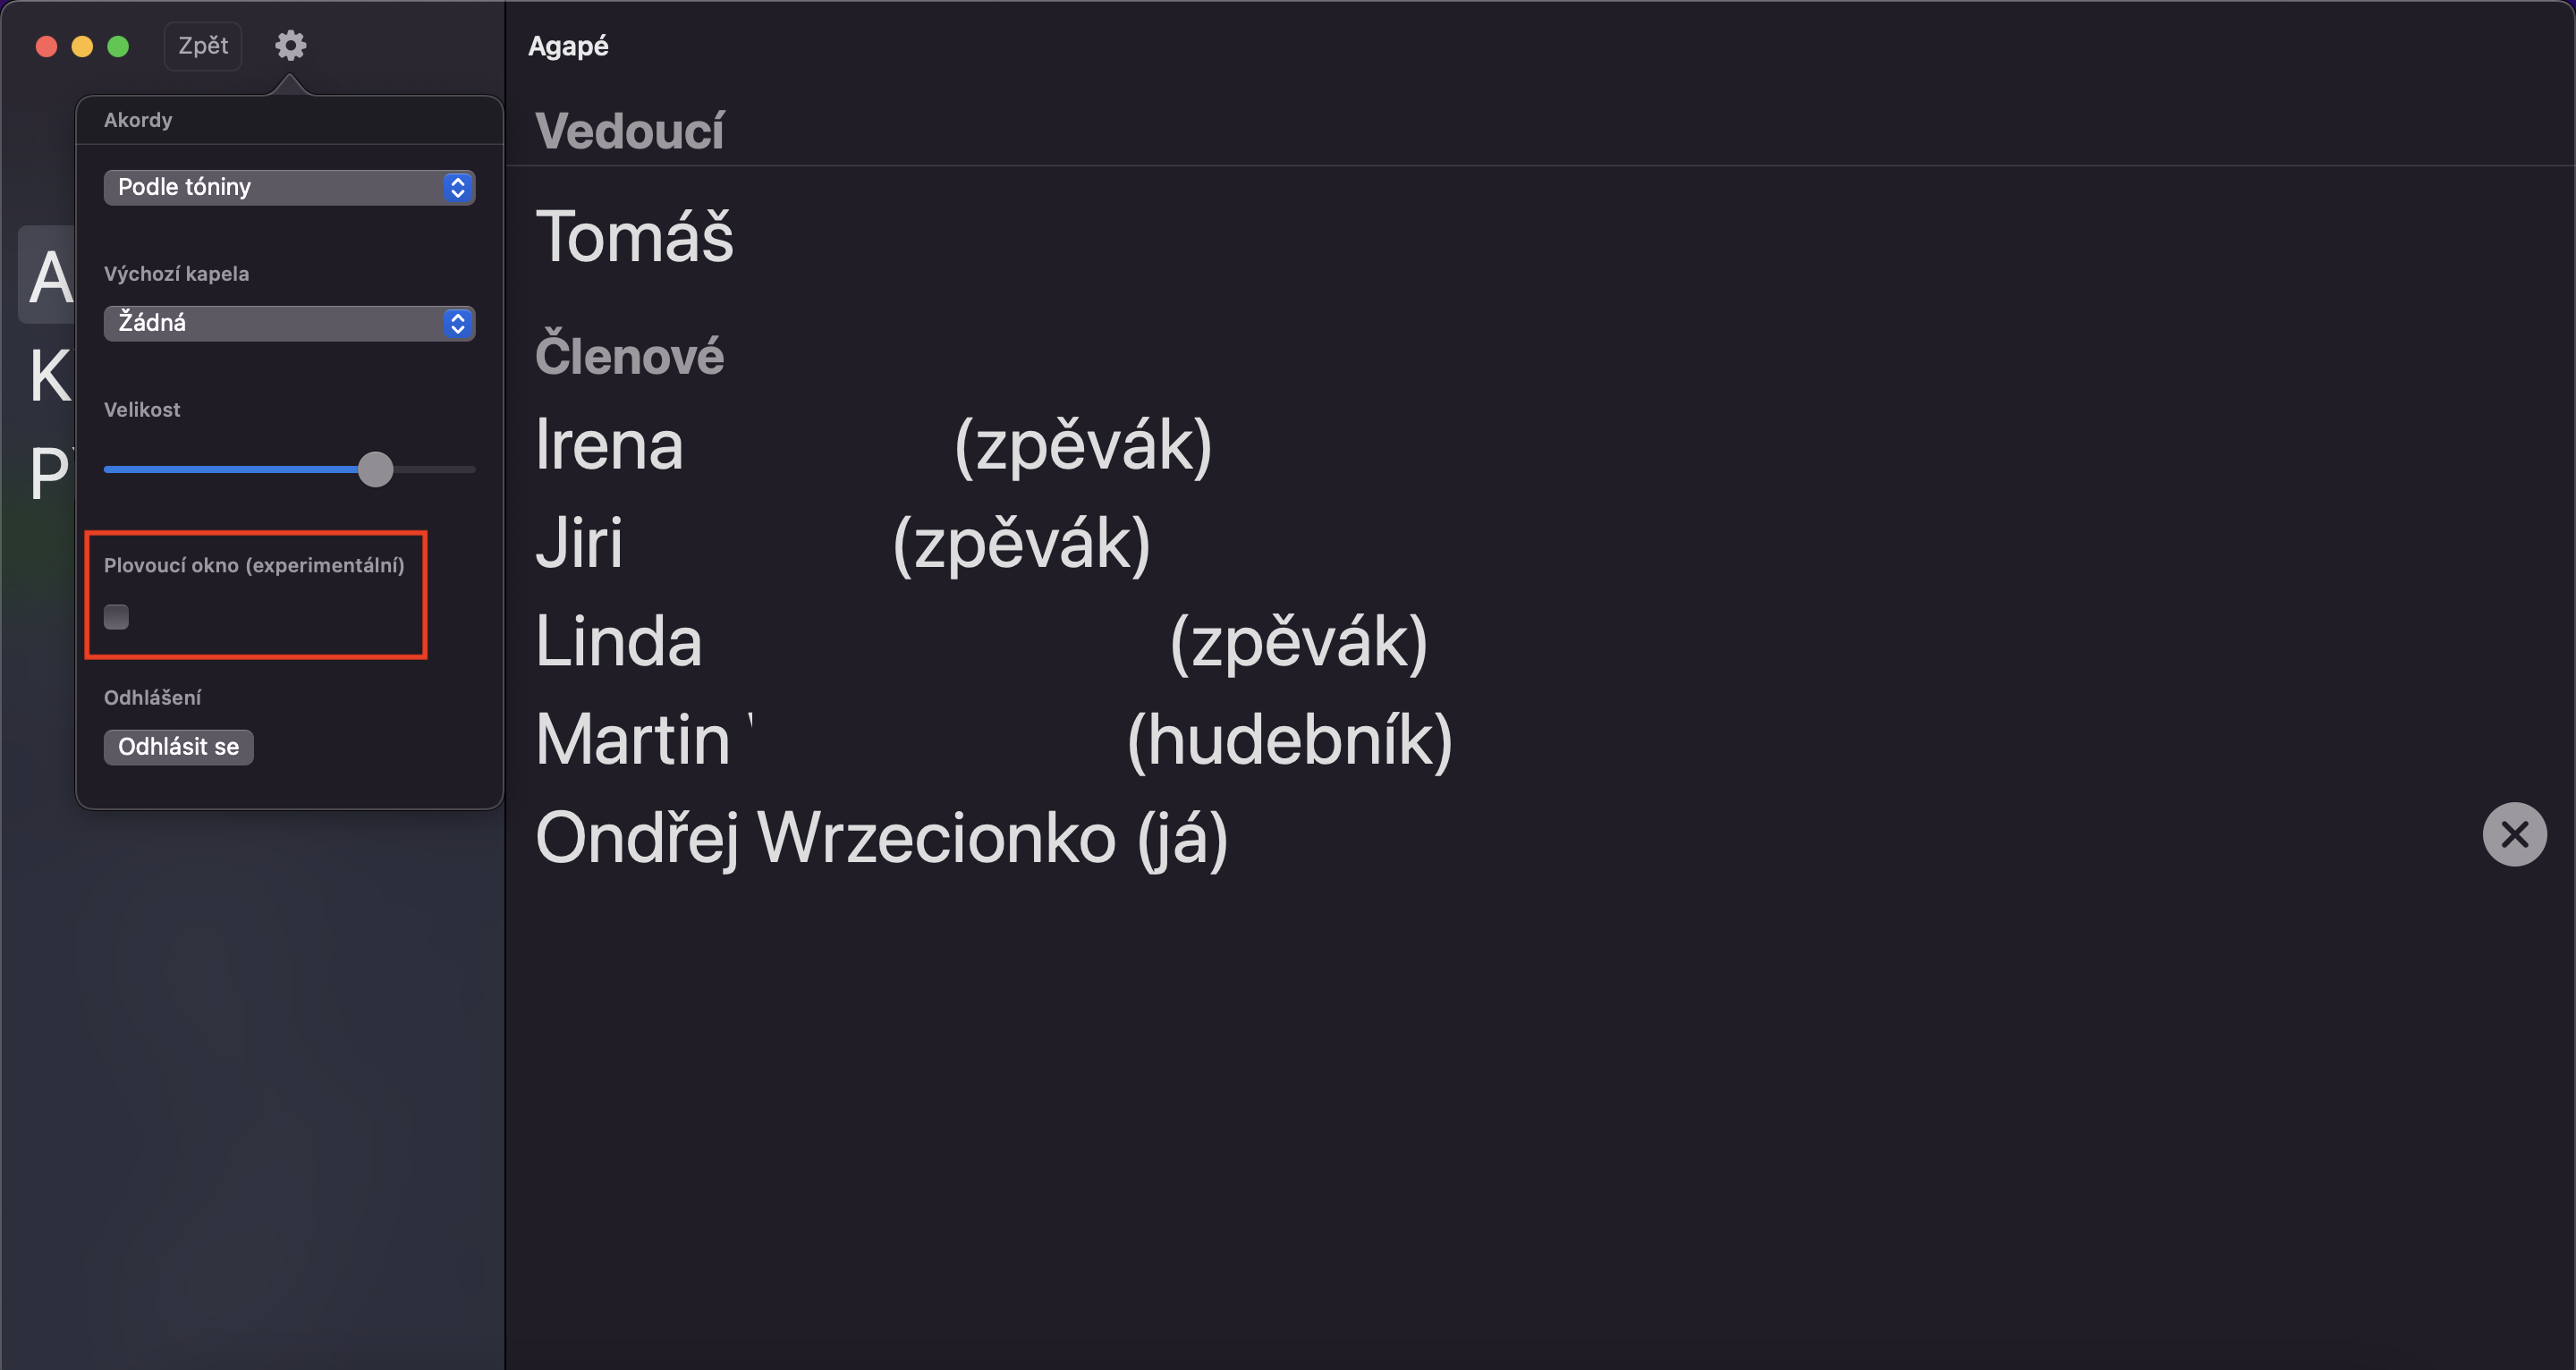
\includegraphics[width=\textwidth]{images/6-testovani/6-7-nastaveni-mac.png}
    \caption[Ukázka obrazovky Nastavení aplikace na macOS]{Nastavení režimu plovoucího okna v aplikaci na operačním systému macOS}
\end{figure}

Další chybou byla absence možnosti znovu načíst seznam písní přímo z aplikace. Po přidání nové písně tak ostatní členové kapely museli aplikaci ukončit a znovu spustit. Tyto chyby jsem vyřešil přidáním tlačítka pro zapnutí režimu plovoucího okna a tlačítka k znovu načtení seznamu písní.

\begin{figure}
    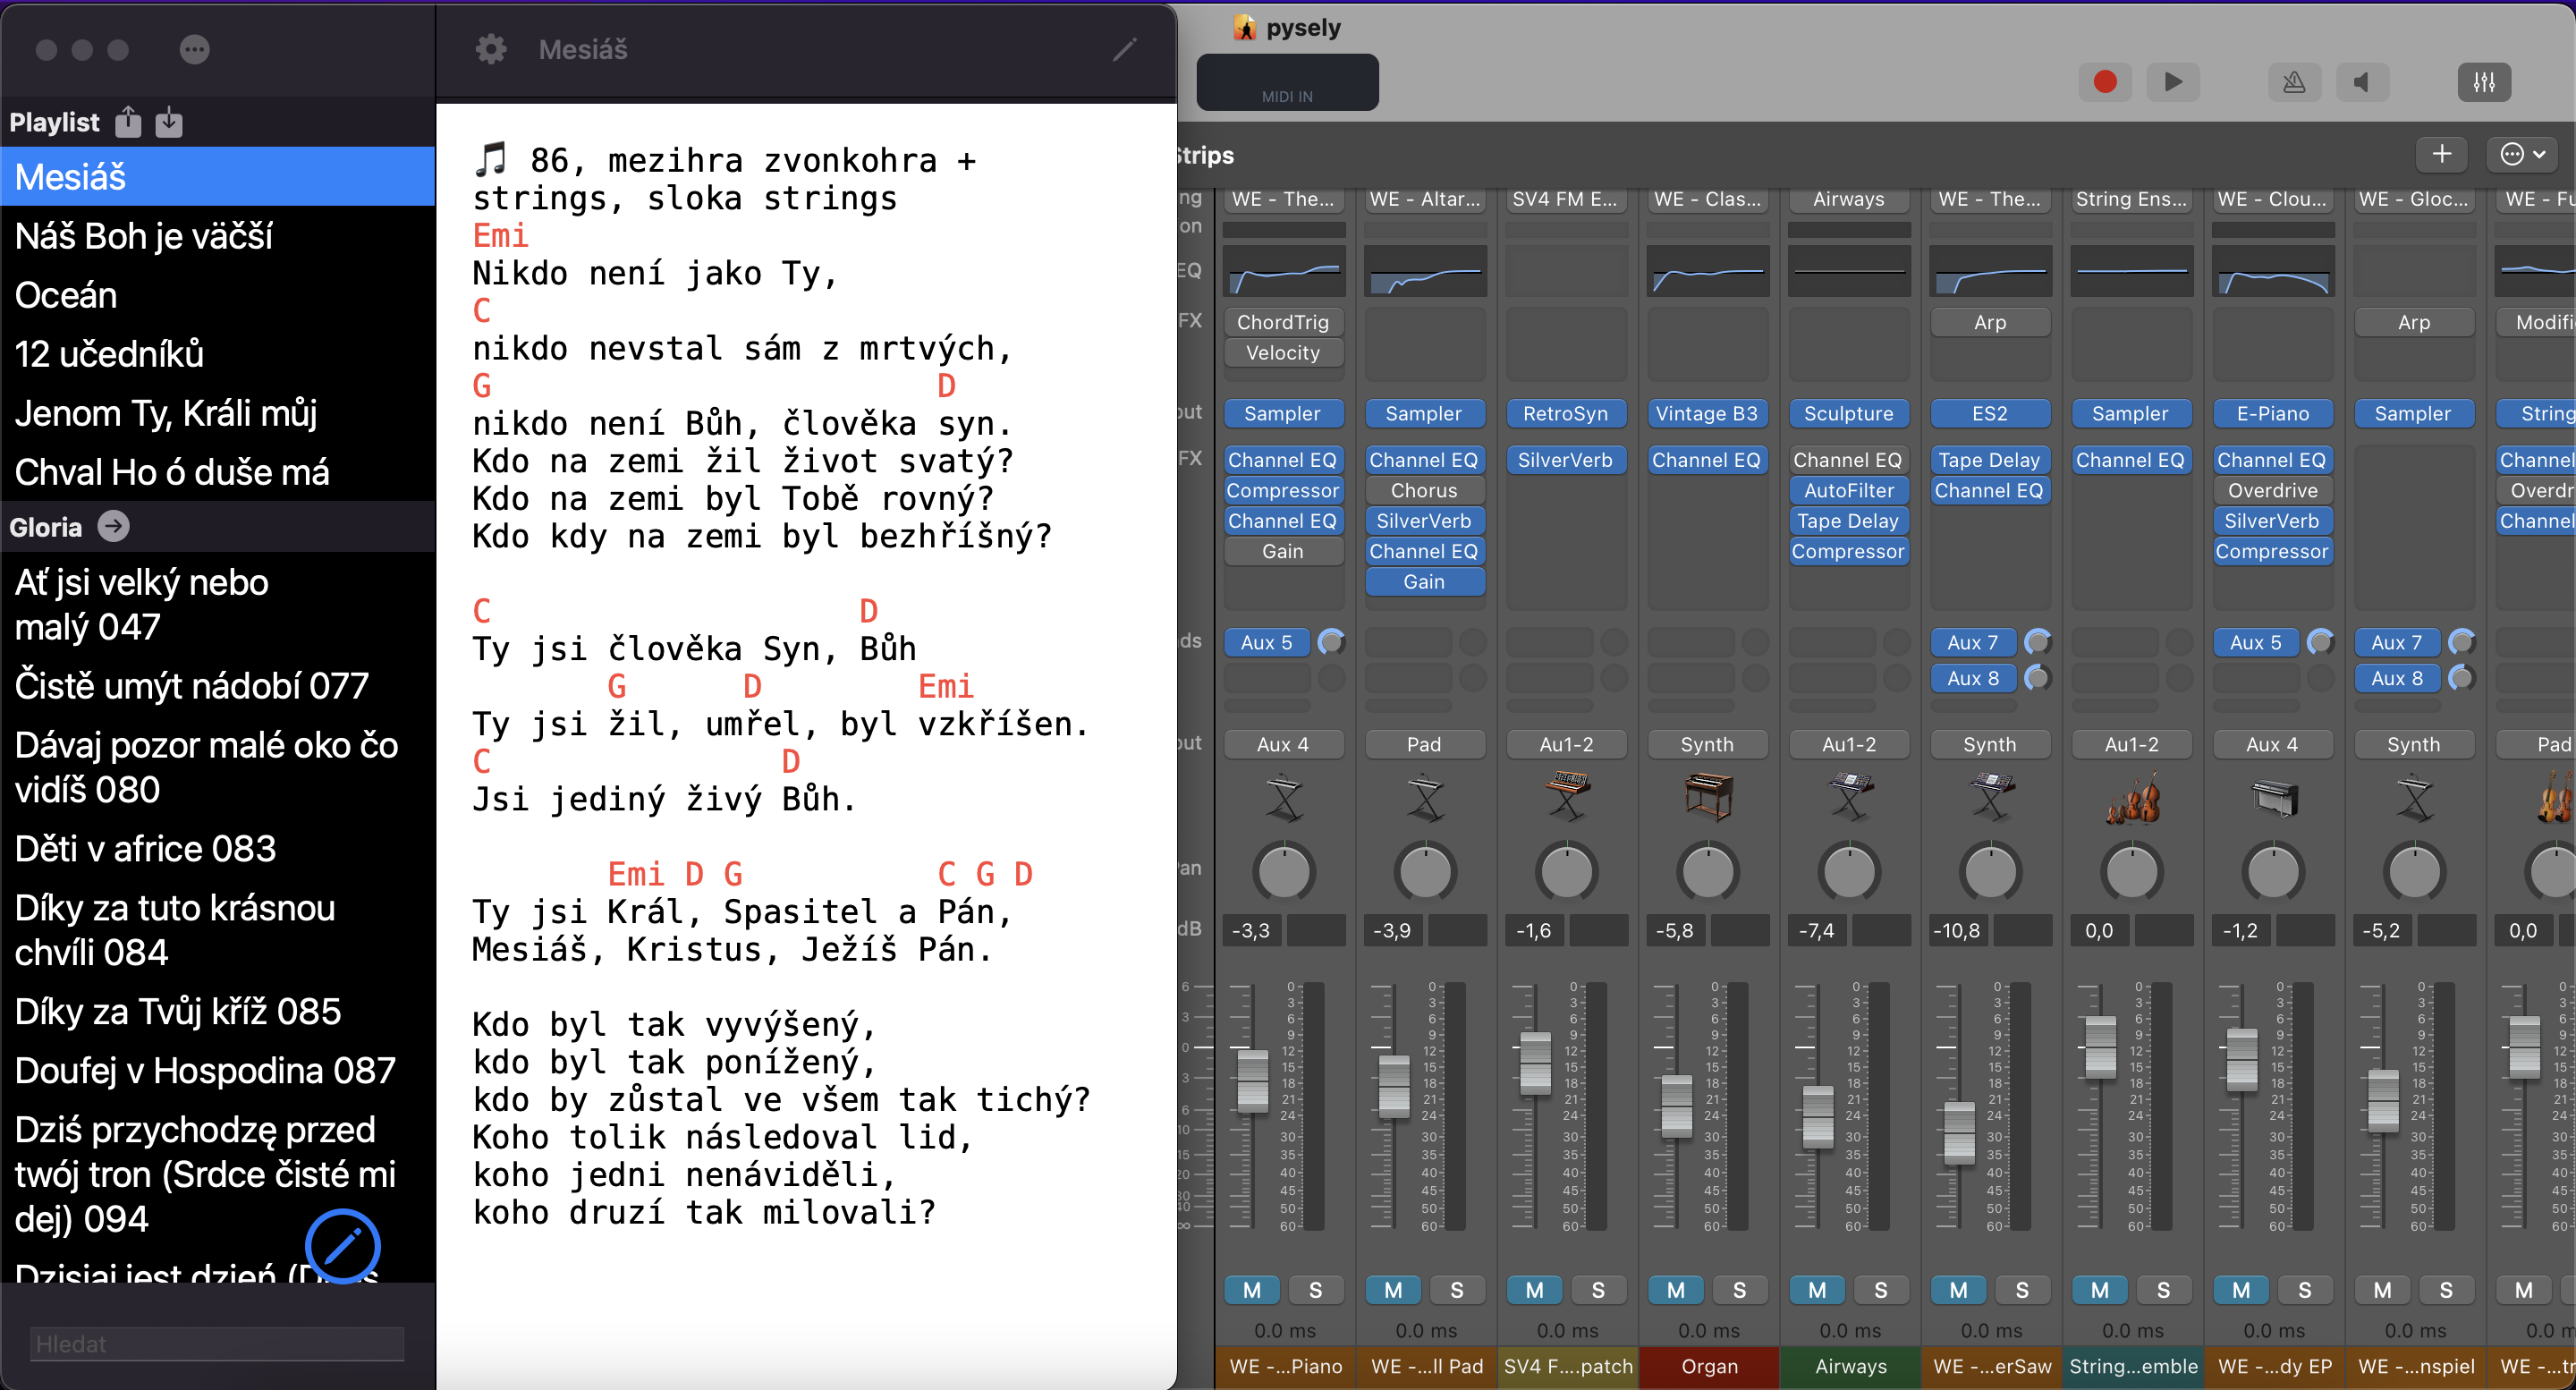
\includegraphics[width=\textwidth]{images/6-testovani/6-8-plovouci-okno.png}
    \caption{Zobrazení aplikace na macOS v režimu plovoucího okna}
\end{figure}

\subsection{Přínos}

V průběhu uživatelských testů jsem dostal mnoho zpětné vazby, díky které jsem mohl odhalit mnoho chyb v aplikaci, kterými byla absence čísla písně ve zpěvníku v názvu písně, nesprávné zobrazení některých komponent ve světlém módu, špatné nahrávání písní do playlistu nebo chybějící možnost znovu načtení seznamu písní. Dostal jsem také konkrétní návrhy na další funkcionality, které by členové hudebního doprovodu využili a které konkrétně popíšu v kapitole \nameref{zaver}.

%---------------------------------------------------------------
\chapter{Nasazení}
%---------------------------------------------------------------

\begin{chapterabstract}
    V této kapitole popíšu proces nasazení serveru na virtuální stroj a nasazení aplikace do obchodu pro iOS/macOS aplikace App Store.
\end{chapterabstract}

\section{Server}

Pro to, aby mohla aplikace s REST API komunikovat, musí být REST API veřejně přístupné, proto jsem se rozhodl jej nasadit na virtuální stroj. U společnosti Hicoria \cite{hicoria} pronajímám virtuální stroj s operačním systémem Debian, 1 GB RAM a 20 GB SSD disku za cenu přibližně 650 Kč ročně. Na tomto stroji již hostuji své webové stránky a dohodl jsem se s náboženskými shromážděními, že tento stroj poskytnu i pro účely nasazení serveru poskytujícího podpůrné REST API.

\begin{figure}[H]
    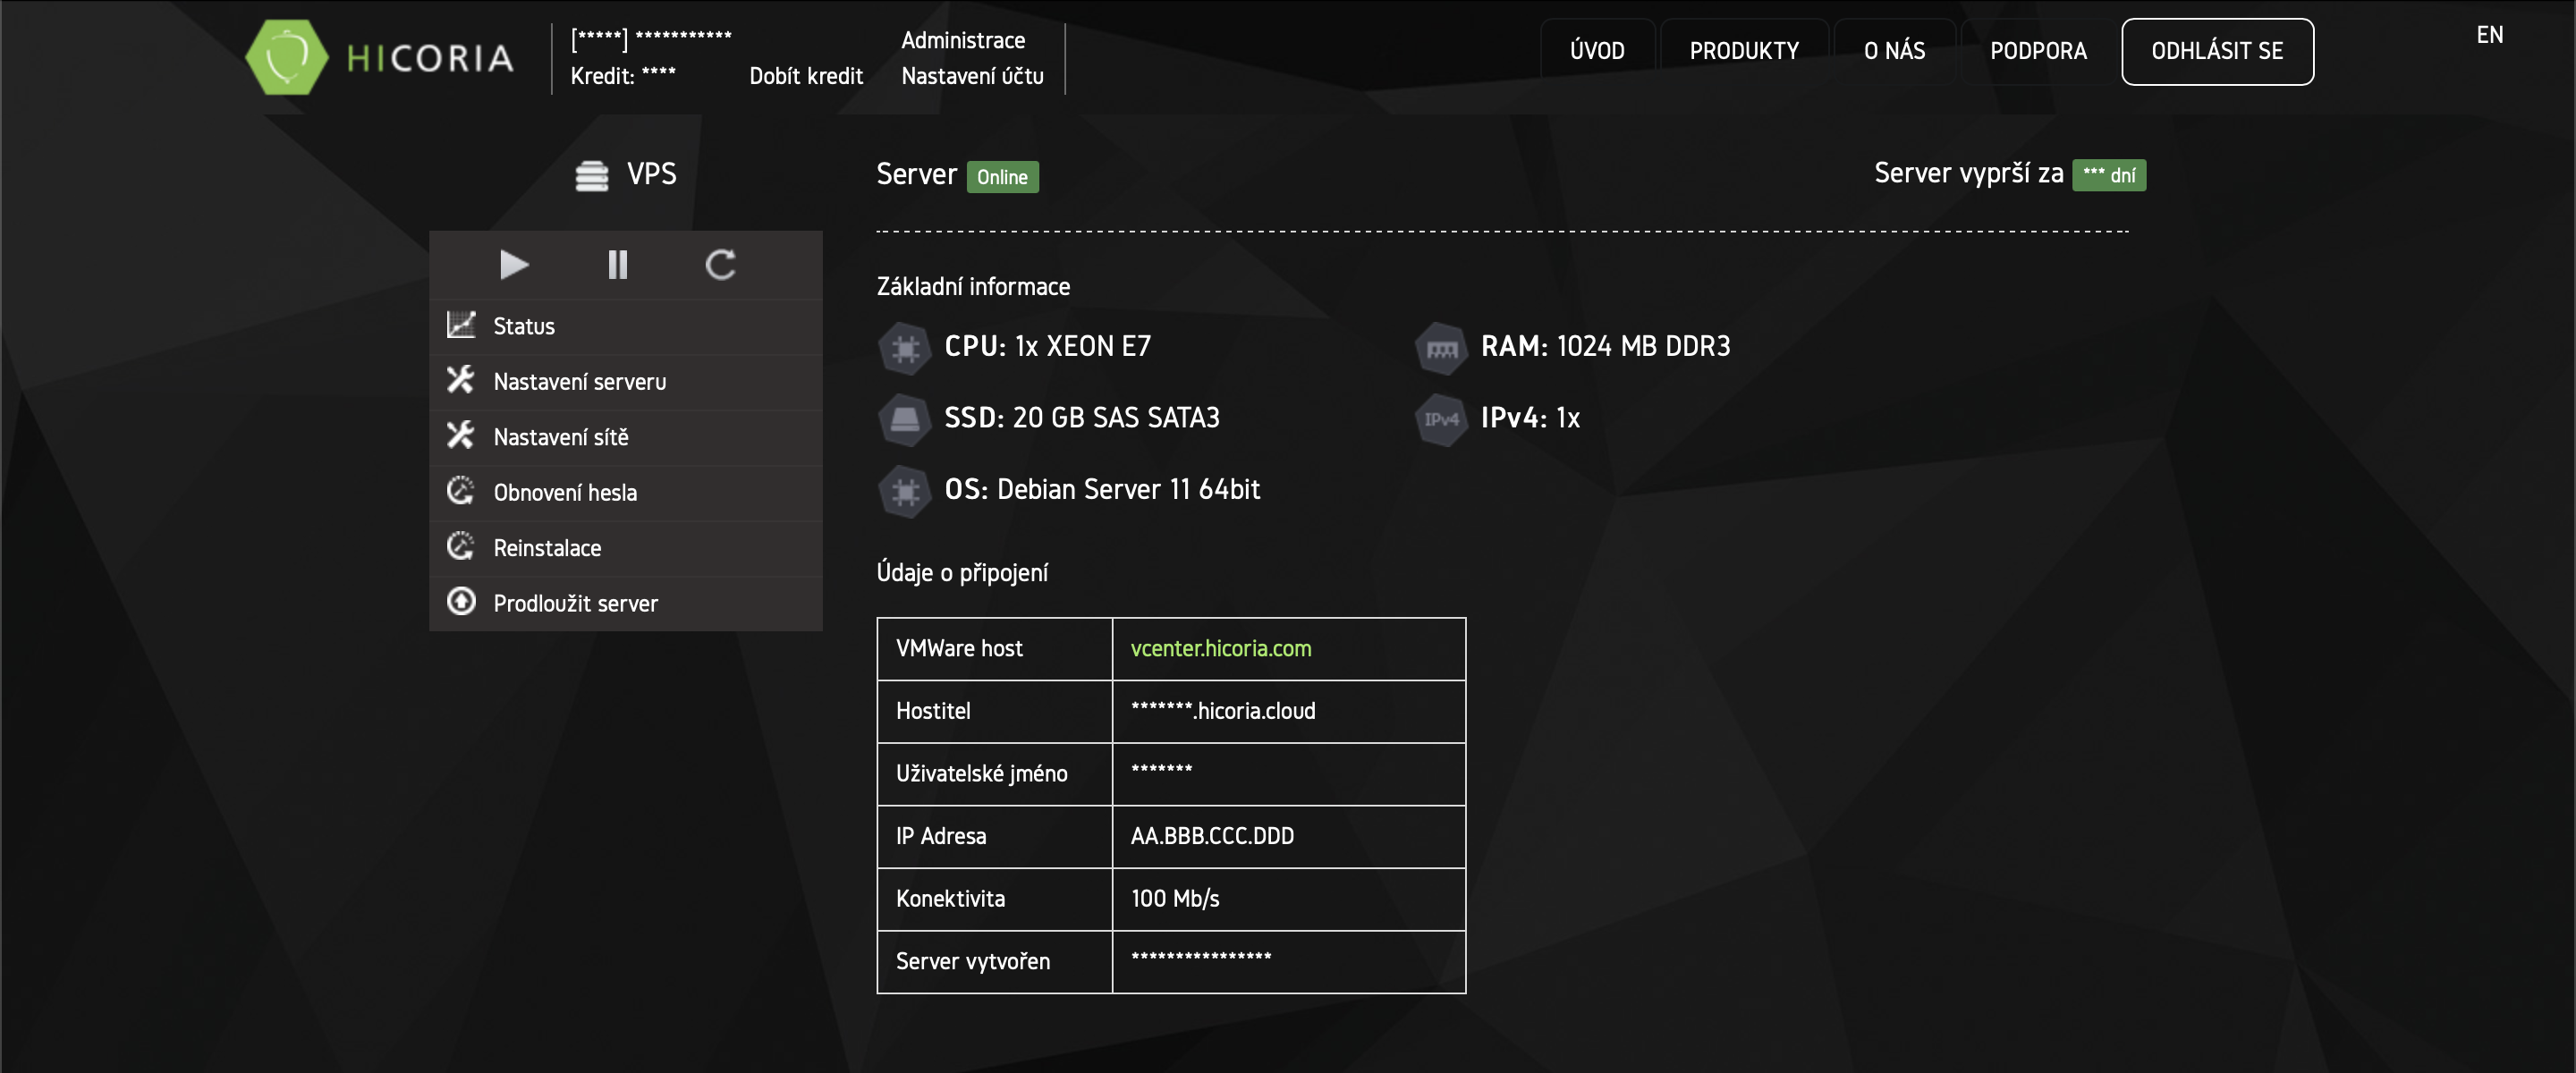
\includegraphics[width=\textwidth]{images/7-nasazeni/7-1-ukazka-hicoria.png}
    \caption{Ukázka administrace virtuálního stroje u společnosti Hicoria}
\end{figure}

Samotné nastavení webového serveru není složité -- stačí nainstalovat Javu, což je s pomocí nástrojů pro Debian jeden příkaz \texttt{sudo apt install default-jdk}. Pro nastavení frameworku Spring Web je následně nutné do konfiguračního souboru \texttt{application.properties} nastavit port, adresu, na které server poběží a také cestu k certifikátu, který bude použit pro HTTPS. Na virtuálním stroji, na který server nasazuji již běží Apache webový server s nastaveným DNS záznamem a HTTPS certifikátem pro doménu \url{https://kvetinac97.cz}, který jsem využil pro účely nasazení API.

\begin{figure}[H]
    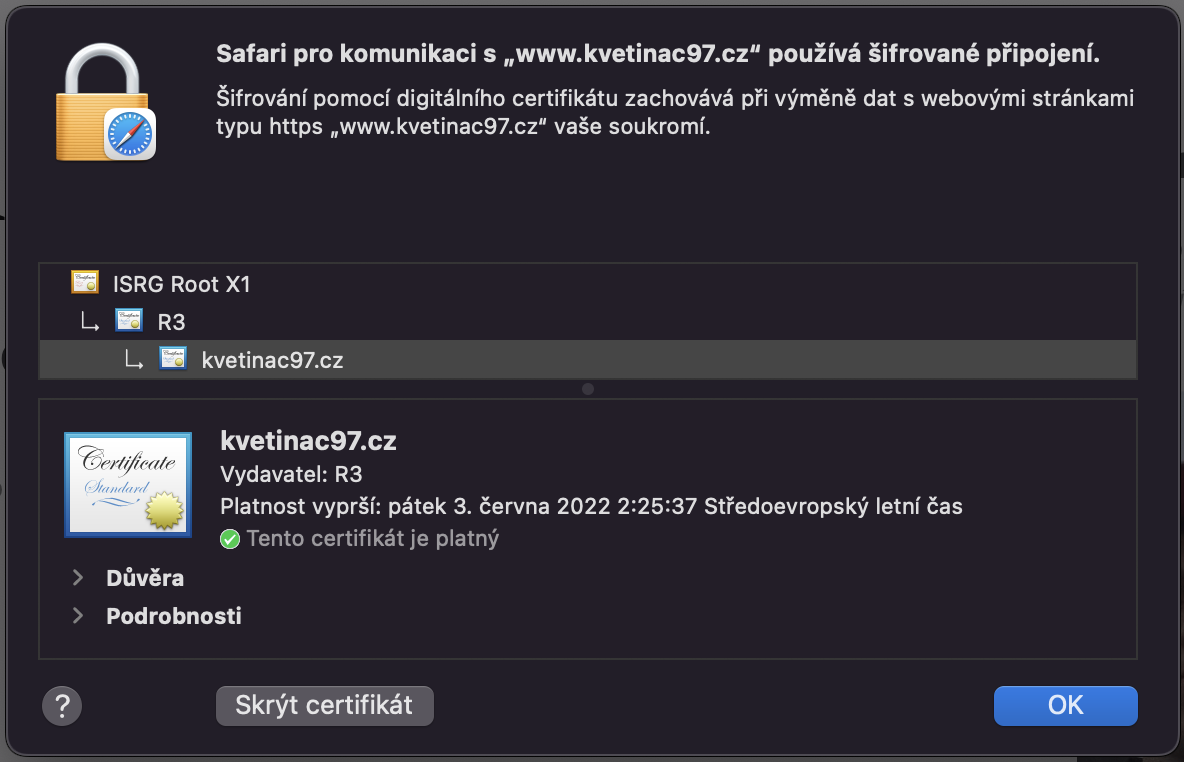
\includegraphics[width=\textwidth]{images/7-nasazeni/7-2-https-server.png}
    \caption[HTTPS certifikát serveru]{HTTPS certifikát serveru na adrese \url{https://kvetinac97.cz}}
\end{figure}

\begin{listing}[H]
\begin{minted}[breaklines,breaksymbolleft=]{properties}
server.port: 8443
security.require-ssl=true
server.ssl.key-store:/etc/letsencrypt/live/kvetinac97.cz/keystore.p12
server.ssl.key-store-password: *****
server.ssl.keyStoreType: PKCS12
server.ssl.keyAlias: *******
\end{minted}
\caption{Konfigurační soubor pro server -- nastavení DNS}
\end{listing}

Aby šlo server spustit, musím zkompilovat kód serveru do spustitelného .jar souboru. Server používá balíčkovací systém Maven \cite{maven}, který obsahuje definici knihoven a závislostí včetně podpůrných knihoven pro Kotlin v konfiguračním souboru \texttt{pom.xml}. Maven obsahuje spustitelný cíl \texttt{mvn package}, který vygeneruje ze zdrojového kódu požadovaný spusitelný soubor ve~formátu jar. Při spuštění serveru je pak důležité server spustit jako systémový proces, aby se po odhlášení uživatele z virtuálního stroje nevypnul, čehož lze jednoduše docílit pomocí POSIX utility \texttt{nohup}. Server je tedy spuštěn příkazem \texttt{nohup java -jar agapesongs.jar \&} a běží na adrese \url{https://kvetinac97.cz:8443}.

\section{App Store}

Jak už jsem psal v kapitole \nameref{testovani}, pro zveřejnění aplikace pro operační systémy iOS a macOS je potřeba tuto aplikaci nahrát do oficiálního obchodu s aplikacemi App Store \cite{app-store}. Stejně jako v případě platformy TestFlight je nejprve potřeba nahrát z programovacího prostředí Xcode verzi aplikace, která musí pro zveřejnění projít schvalovacím procesem App Review. Narozdíl od~TestFlight kontroly je ale tento proces mnohem důkladnější a může se tedy stát, že verze, která projde TestFlight kontrolou, neprojde App Store kontrolou. Po nahrání verze je třeba vyplnit záznam aplikace na platformě App Store Connect \cite{app-store-connect}. Záznam aplikace obsahuje snímky obrazovky, popis a další metadata aplikace. Při kontrole App Review se pak kromě kontroly aplikace samotné kontroluje také záznam v obchodě a jeho soulad s nahranou aplikací.

\begin{figure}
    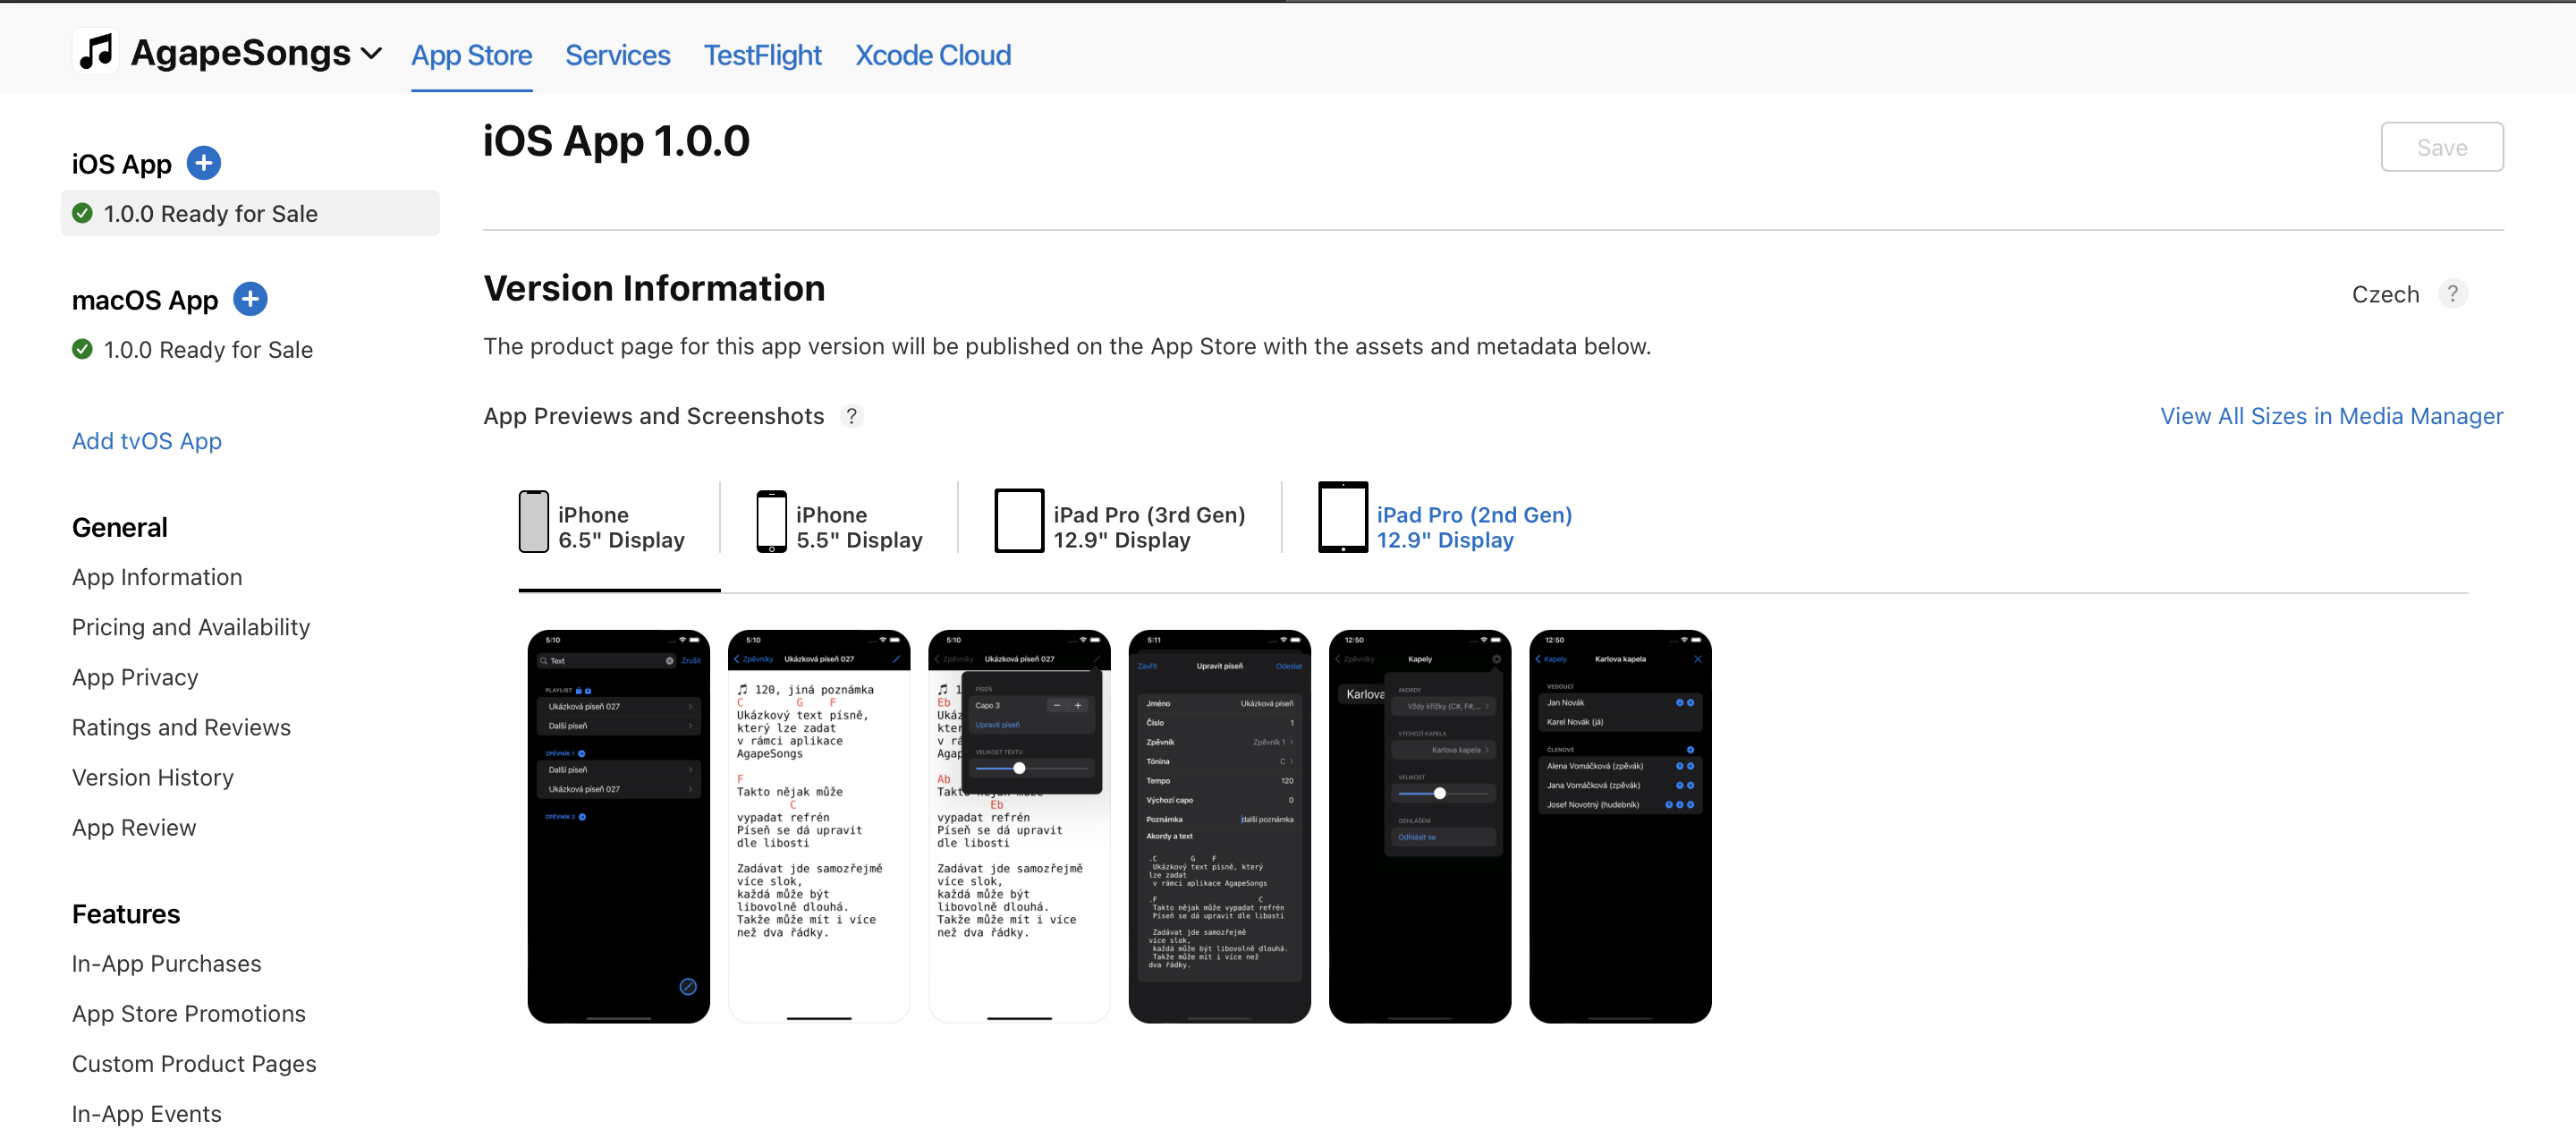
\includegraphics[width=\textwidth]{images/7-nasazeni/7-3-appstore.png}
    \caption{Úvodní obrazovka aplikace v App Store Connect}
\end{figure}

Z vlastních zkušeností z nahrávání aplikací do App Store jsem se pro jistotu rozhodl zkusit nahrát první verzi aplikace už ve čtvrtek 14. 4. 2022. V pátek 15. 4. 2022 mi byla zamítnuta jak iOS, tak macOS verze aplikace. U iOS verze bylo problémem příliš velké tlačítko pro přihlášení přes Apple, což jsem vyřešil změnou jeho velikosti. U macOS bylo problémem označení, že je aplikace serverem (budou se k ní připojovat zařízení ze sítě), i když neumožňuje přijímat příchozí připojení. Toto označení jsem tedy odstranil.

\begin{figure}[H]
    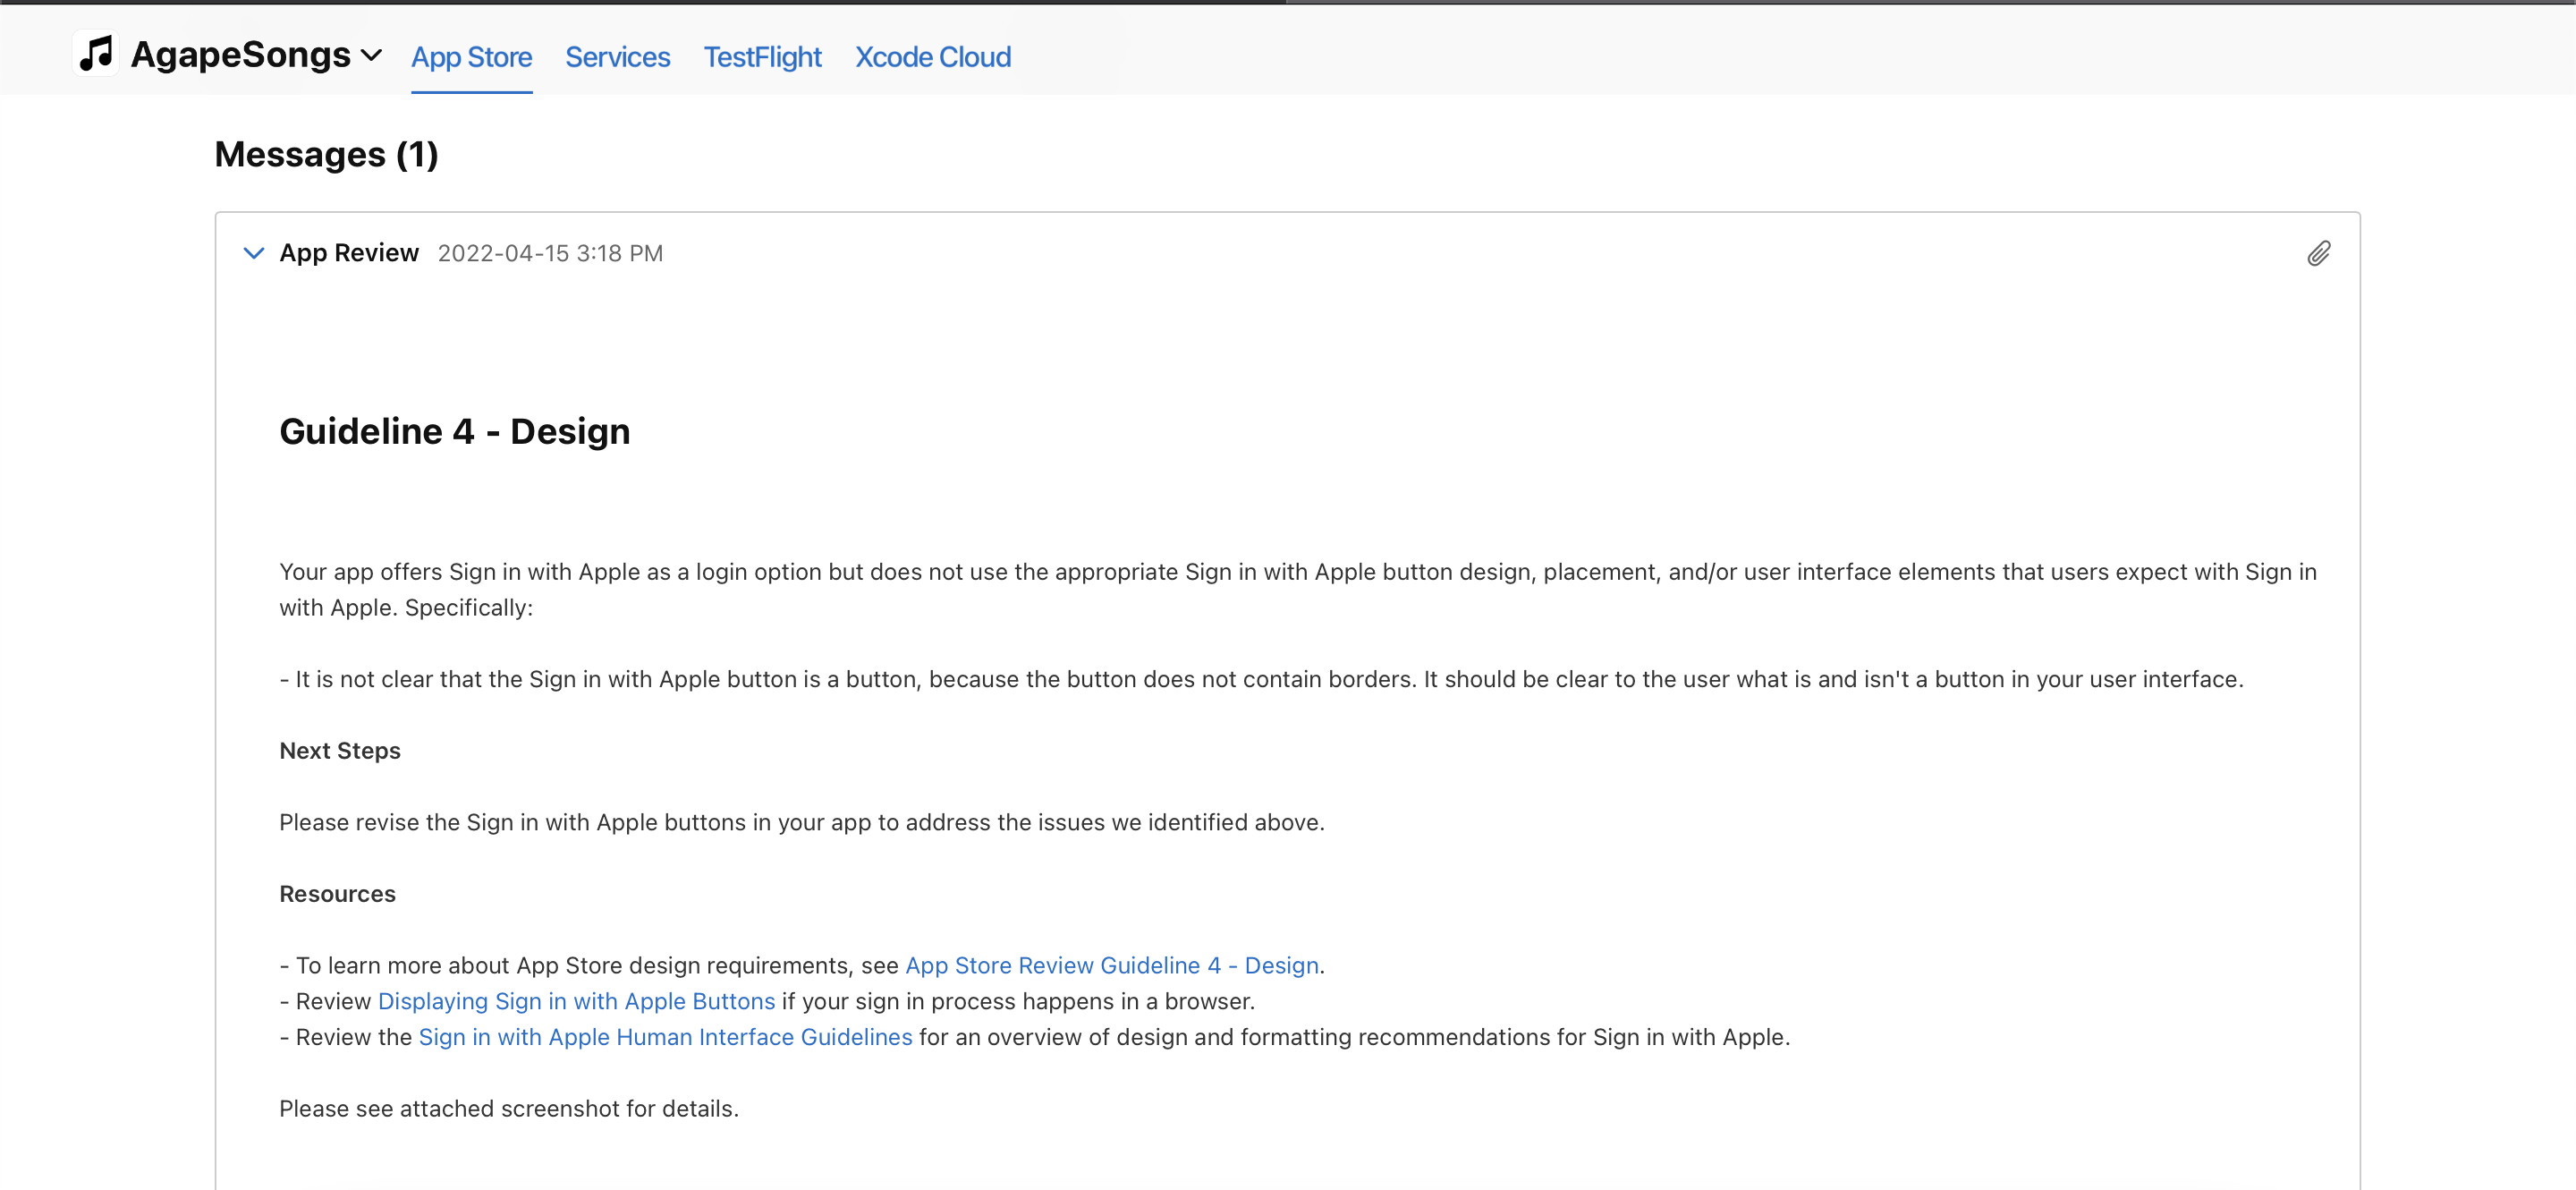
\includegraphics[width=\textwidth]{images/7-nasazeni/7-4-appstore-zamitnuti.png}
    \caption{Informace o zamítnutí aplikace při kontrole App Review}
\end{figure}

Po zmíněných úpravách již aplikace pro obě dvě platformy kontrolou prošly a mohl jsem je vydat veřejně. Jak iOS, tak macOS aplikace jsou tedy veřejně dostupné ke stažení v obchodu pro aplikace App Store.

\begin{figure}[H]
    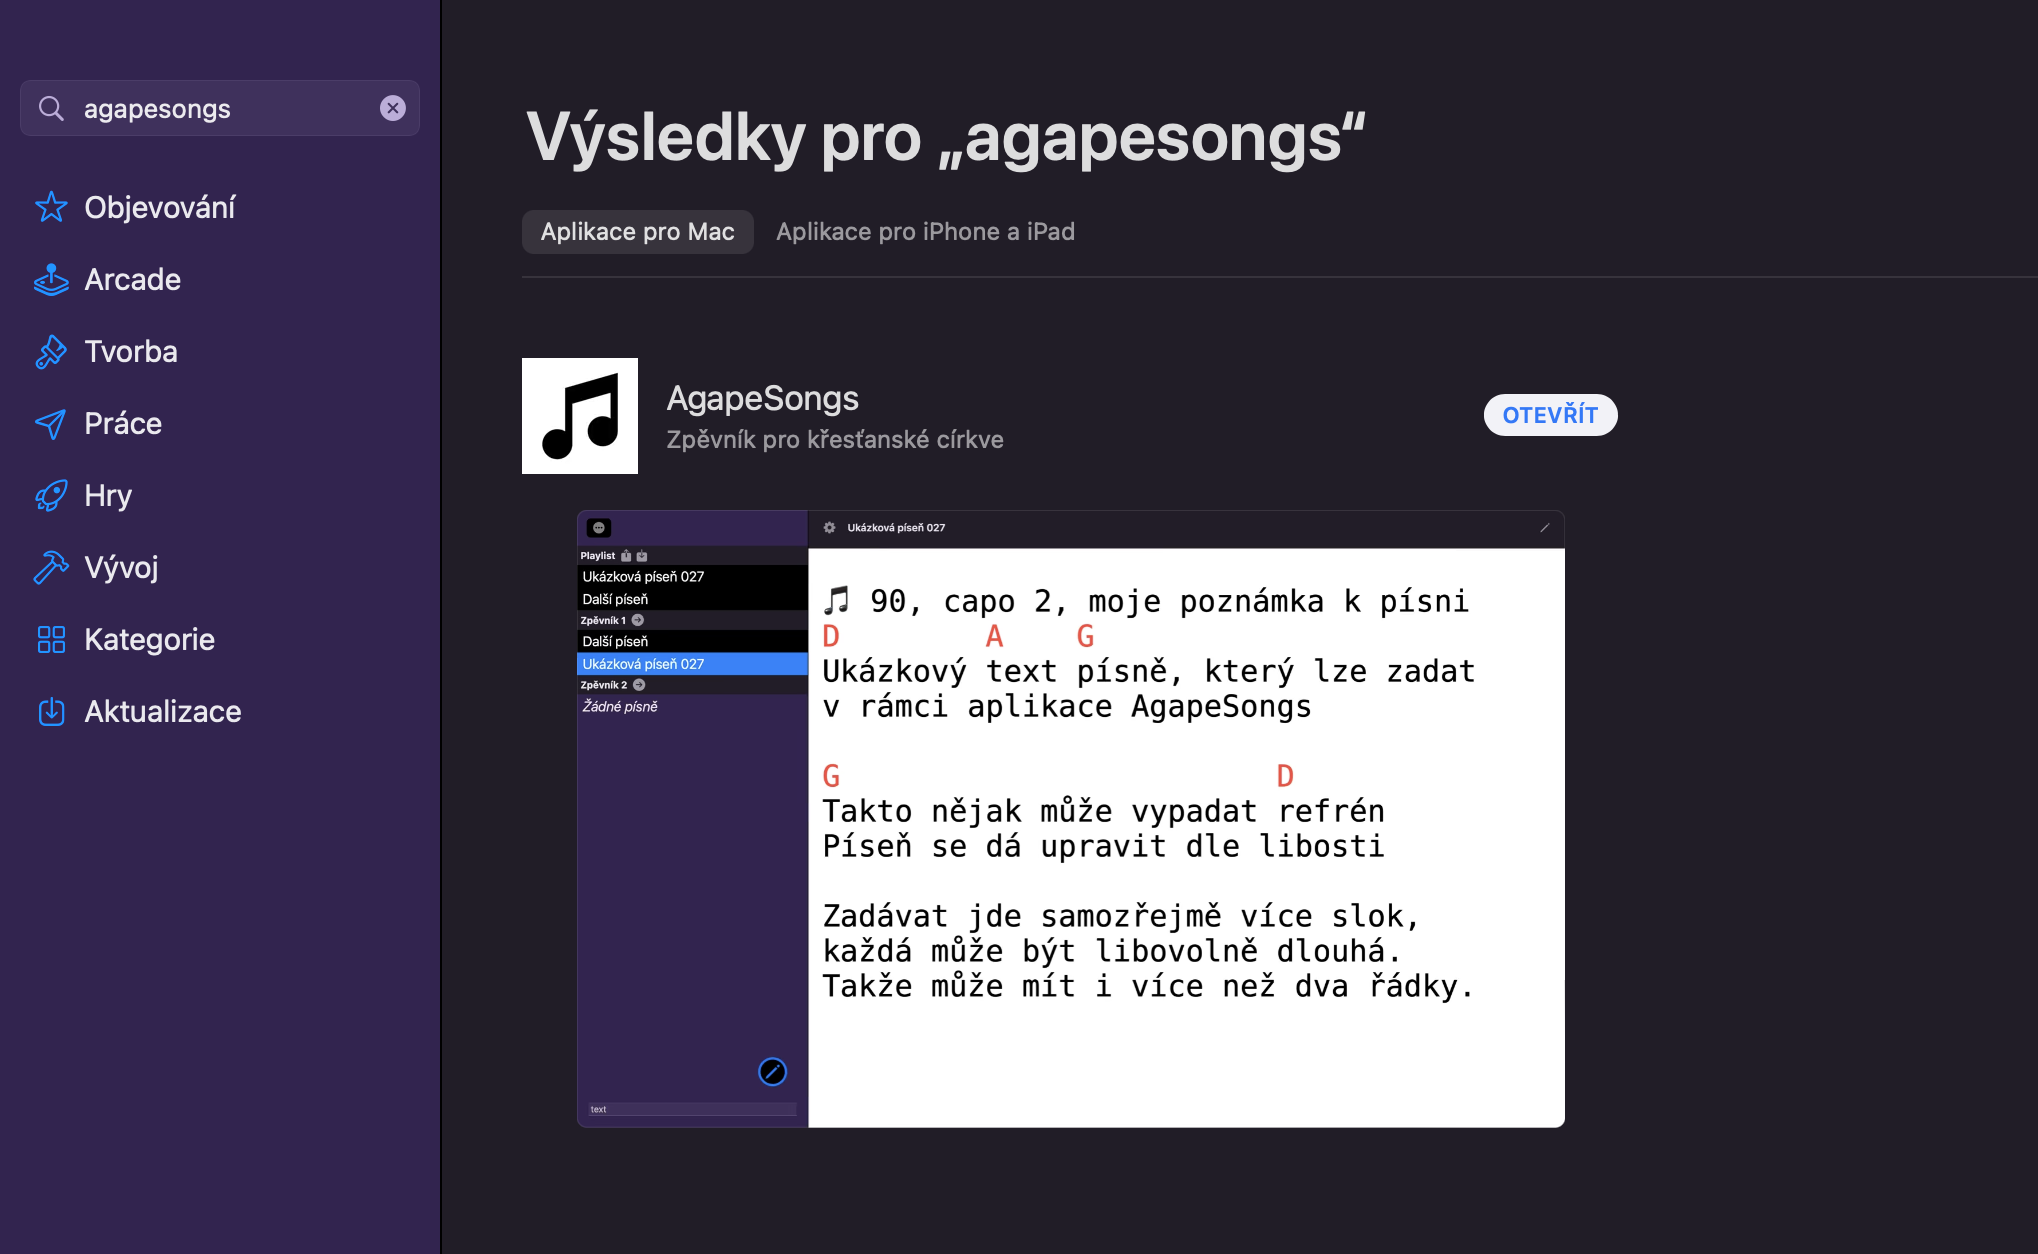
\includegraphics[width=\textwidth]{images/7-nasazeni/7-5-appstore-mac.png}
    \caption{Ukázka aplikace v obchodu pro macOS aplikace App Store}
\end{figure}

\begin{figure}[H]
    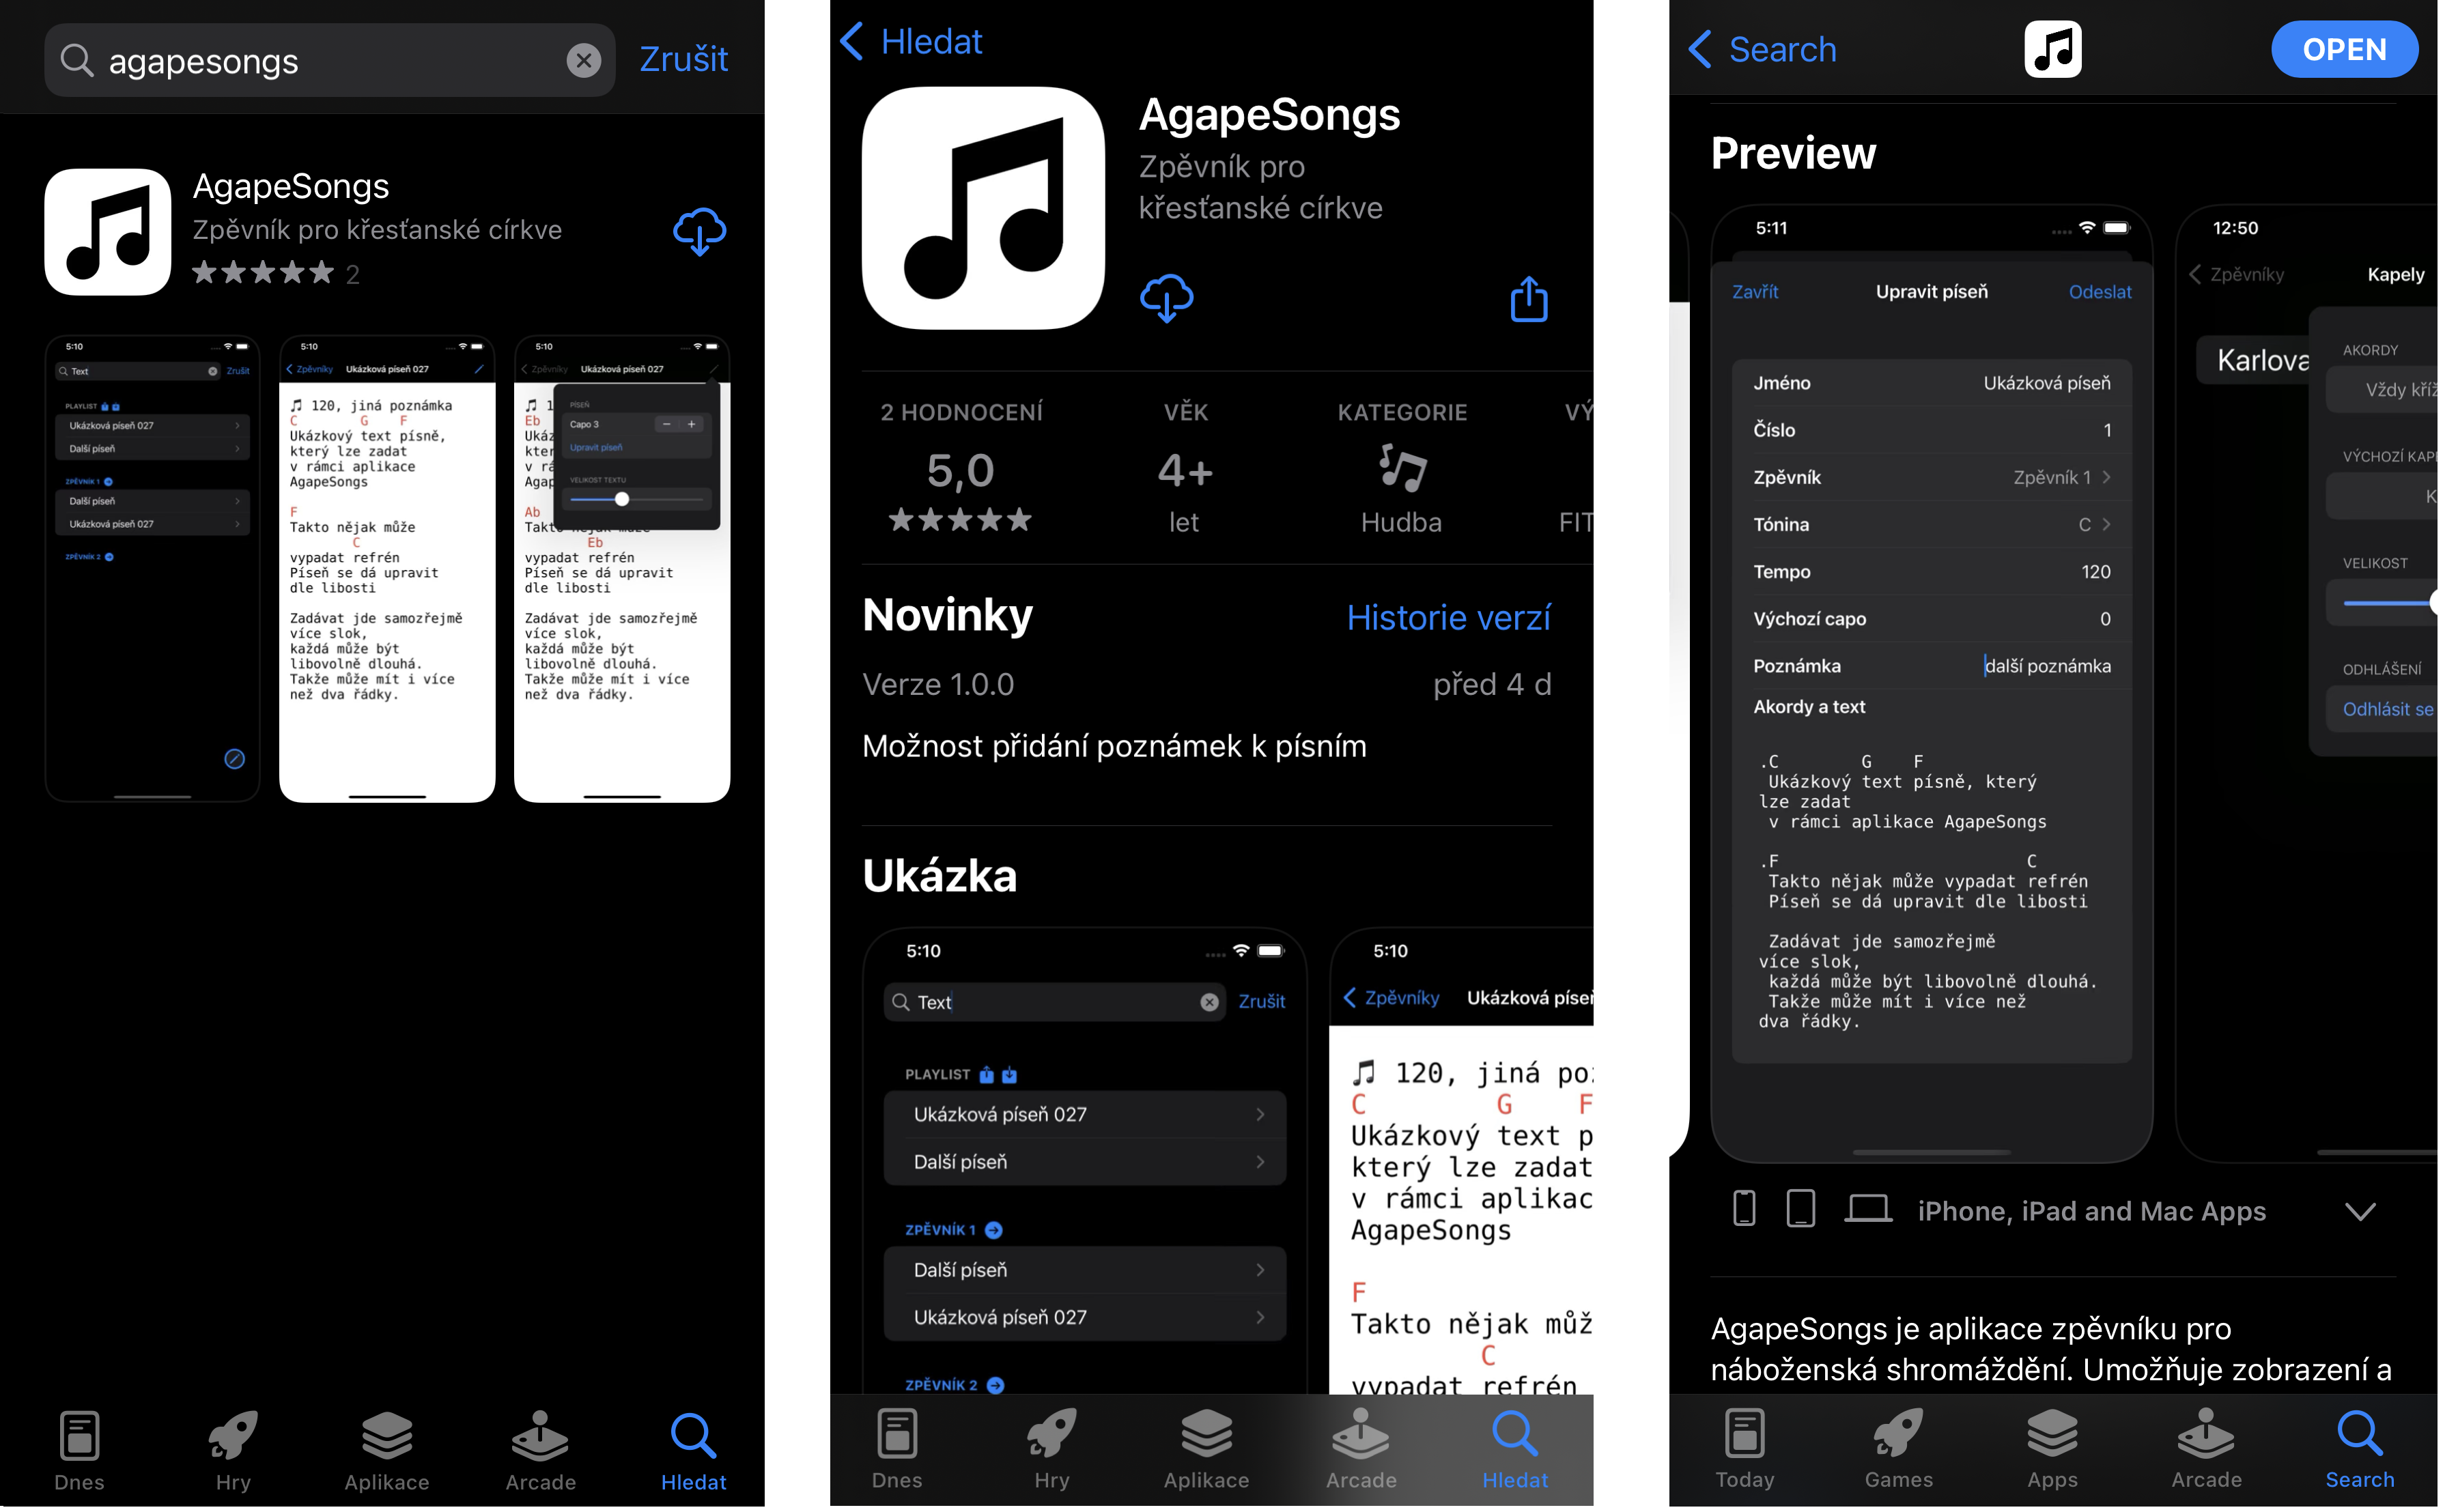
\includegraphics[width=\textwidth]{images/7-nasazeni/7-6-appstore-ios.png}
    \caption{Ukázka aplikace v obchodu pro iOS aplikace App Store}
\end{figure}

%---------------------------------------------------------------
\chapter*{Závěr}
\addcontentsline{toc}{chapter}{Závěr}
\markboth{Závěr}{Závěr}
\label{zaver}
%---------------------------------------------------------------

Ve své práci jsem se zabýval tvorbou mobilní aplikace zpěvníku pro náboženská shromáždění. Provedl jsem analýzu stávajících řešení přípravy a koordinace zpěvu věřících a hudebního doprovodu, z čehož jsem zjistil, že stávající řešení promítače pro koordinaci zpěvu věřících a hudebního doprovodu náboženským shromážděním vyhovuje, zatímco stávající řešení papírového zpěvníku pro přípravu písní není dostačující. Na základě zjištěných informací jsem aplikaci navrhl jako serverovou část v programovacím jazyce Kotlin s použitím technologie Spring Web a klientskou část v podobě iOS a macOS aplikace v programovacím jazyce Swift.

V průběhu implementace jsem narazil na více problémů, mezi které patřilo zalamování zobrazovaného textu, transpozice akordů a multiplatformnost aplikace. iOS a macOS aplikace a podpůrný server jsem přesto naprogramoval a otestoval s pomocí jednotkových testů, REST API jsem otestoval pomocí integračních testů v programu Postman a aplikaci jako celek jsem nakonec otestoval uživatelsky.

Výslednou aplikaci jsem nasadil do obchodu pro iOS a macOS aplikace App Store, ze kterého ji za první měsíc nainstalovala a začala používat náboženská shromáždění v Českém Těšíně i Pyšelích, která do ní dosud nahrála přes 1000 písní v 10 zpěvnících a jsou s aplikací, stejně jako já, spokojeni. Domluvili jsme se proto s těmito shromážděními na pokračující údržbě aplikace a také na propagaci v časopise pro Křesťanské sbory a na webových stránkách Křesťanských sborů.

\section*{Budoucí rozšíření}

V průběhu analýzy, vývoje a testování aplikace jsem od členů kapely dostal mnoho návrhů, které jsem z časových důvodů nemohl všechny do aplikace zahrnout. Mezi ty nejdůležitější patří:

\textbf{Možnost úprav bez připojení k internetu}: V průběhu analýzy jsem zjistil, že je ve~všech náboženských shromážděních dostupné připojení k internetu. Náboženská shromáždění ale během roku pořádají různé akce a tábory, které se často konají v přírodě bez připojení k internetu a pokud v průběhu akce člen hudebního doprovodu nalezne v písni nesprávný akord, nemá možnost jej opravit.

Aplikace by tedy mohla podporovat úpravu písní i bez připojení k internetu. V takovém případě by se změna uložila lokálně a byla by na server nahrána až ve chvíli, kdy bude zařízení připojeno k internetu.

\textbf{Synchronizace playlistů v reálném čase}: V aplikaci jsem implementoval synchronizaci playlistů v podobě tlačítek umožňujících nahrání a stažení playlistu do příslušné kapely včetně možnosti automatického nahrávání všech změn v playlistu do zvolené výchozí kapely. Stále zde ale pro hudebníky zůstává nutnost znovu stáhnout playlist poté, co v něm vedoucí kapely provede změnu. Aplikace by tedy mohla nabídnout zvolení výchozí kapely, ze které by se v reálném čase stahoval playlist a hudebníci by si tak nemuseli po každé změně playlist znovu stahovat.

\textbf{Podpora více verzí a překladů jedné písně}: Některé z písní, které shromáždění zpívají, jsou dostupné v různých verzích a překladech -- některá shromáždění píseň zpívají česky, některá polsky, některá slovensky. V aktuálním stavu musí být každá verze písně do aplikace přidána jako nová píseň. Jedním z možných budoucích rozšíření je tedy přidávání více jazykových verzí písně, kdy následně mezi jednotlivými verzemi budou uživatelé přepínat v nastavení písně.

\textbf{Podpora poznámek i v textu písně}: Aktuální verze aplikace podporuje přidávání soukromých poznámek k písni. Tyto poznámky se následně ukážou na začátku textu písně spolu s~informacemi o tempu písně nebo výchozí transpozici. Tento formát poznámek je zcela dostačující například pro zaznamenání rejstříku, který bude hudebník pro danou píseň používat. V této verzi si ale hudebník nemůže zaznamenat poznámku přímo k řádku, na kterém má přepnout rejstřík. Další funkcionalitou, kterou by tak aplikace mohla v budoucnu poskytnout, je zápis poznámek kdekoliv v textu písně a možnost psát poznámky s pomocí stylusu Apple Pencil.

\textbf{Podpora více oken na platformě macOS}: Někteří členové kapely, kteří využívají aplikaci na operačním systému macOS, jsou zvyklí využívat aplikace v režimu více oken, případně využívají možnost použití více panelů v jednom okně. Aplikace by tedy mohla podporovat zobrazení více písní ve více oknech a otevření více písní ve více panelech v jednom okně.

\textbf{Možnost tisku písní přímo z aplikace}: Ve stávající verzi aplikace můžou členové kapely stáhnout ze serveru píseň jako textový soubor, který mohou následně poslat dalším uživatelům nebo vytisknout. Aplikace by ale mohla nabídnout tisk formou nativního dialogu přímo z iPhonu, iPadu nebo MacBooku.

\textbf{Webová stránka a iOS aplikace pro zobrazení aktuálně přehrávané písně věřícím}: V průběhu analýzy jsem vyhodnotil stávající řešení koordinace zpěvu a hudebního doprovodu jako dostačující a tvorbu vlastního řešení jsem zavrhnul, jelikož by plně nenahradilo používané řešení promítače. Někteří věřící a především promítač by ale uvítali webovou stránku nebo iOS aplikaci, která by zobrazovala text aktuálně přehrávané písně.

\textbf{Pomocná Android a Windows aplikace pro synchronizaci s aplikací OpenSong}: Při analýze jsem došel k závěru, že budu aplikaci koncipovat pro operační systémy iOS a \mbox{macOS} mimojiné také proto, že na platformách Windows a Android již existuje řešení OpenSong, které náboženským shromážděním s menšími výhradami vyhovuje. V budoucnu bych mohl vytvořit podpůrnou aplikaci, která by prováděla synchronizaci písní mezi řešením OpenSong a API rozhraním mé aplikace.


% include appendix
\appendix\appendixinit
\chapter{Návrh REST API}

Součástí bakalářské práce je také návrh REST API pro komunikaci mobilní aplikace s podpůrným serverem. API jsem navrhl pomocí editoru Swagger \cite{swagger} a je dostupné na přiloženém CD v~souboru s názvem \texttt{rest.yaml}.

Po vložení přiloženého YAML souboru na webové stránce \url{https://editor.swagger.io} v~záložce File -- Import file je vygenerována interaktivní dokumentace včetně popisu jednotlivých endpointů, potřebných parametrů, způsobu autorizace a návratových kódů.

\vspace*{1in}

\begin{figure}[H]
    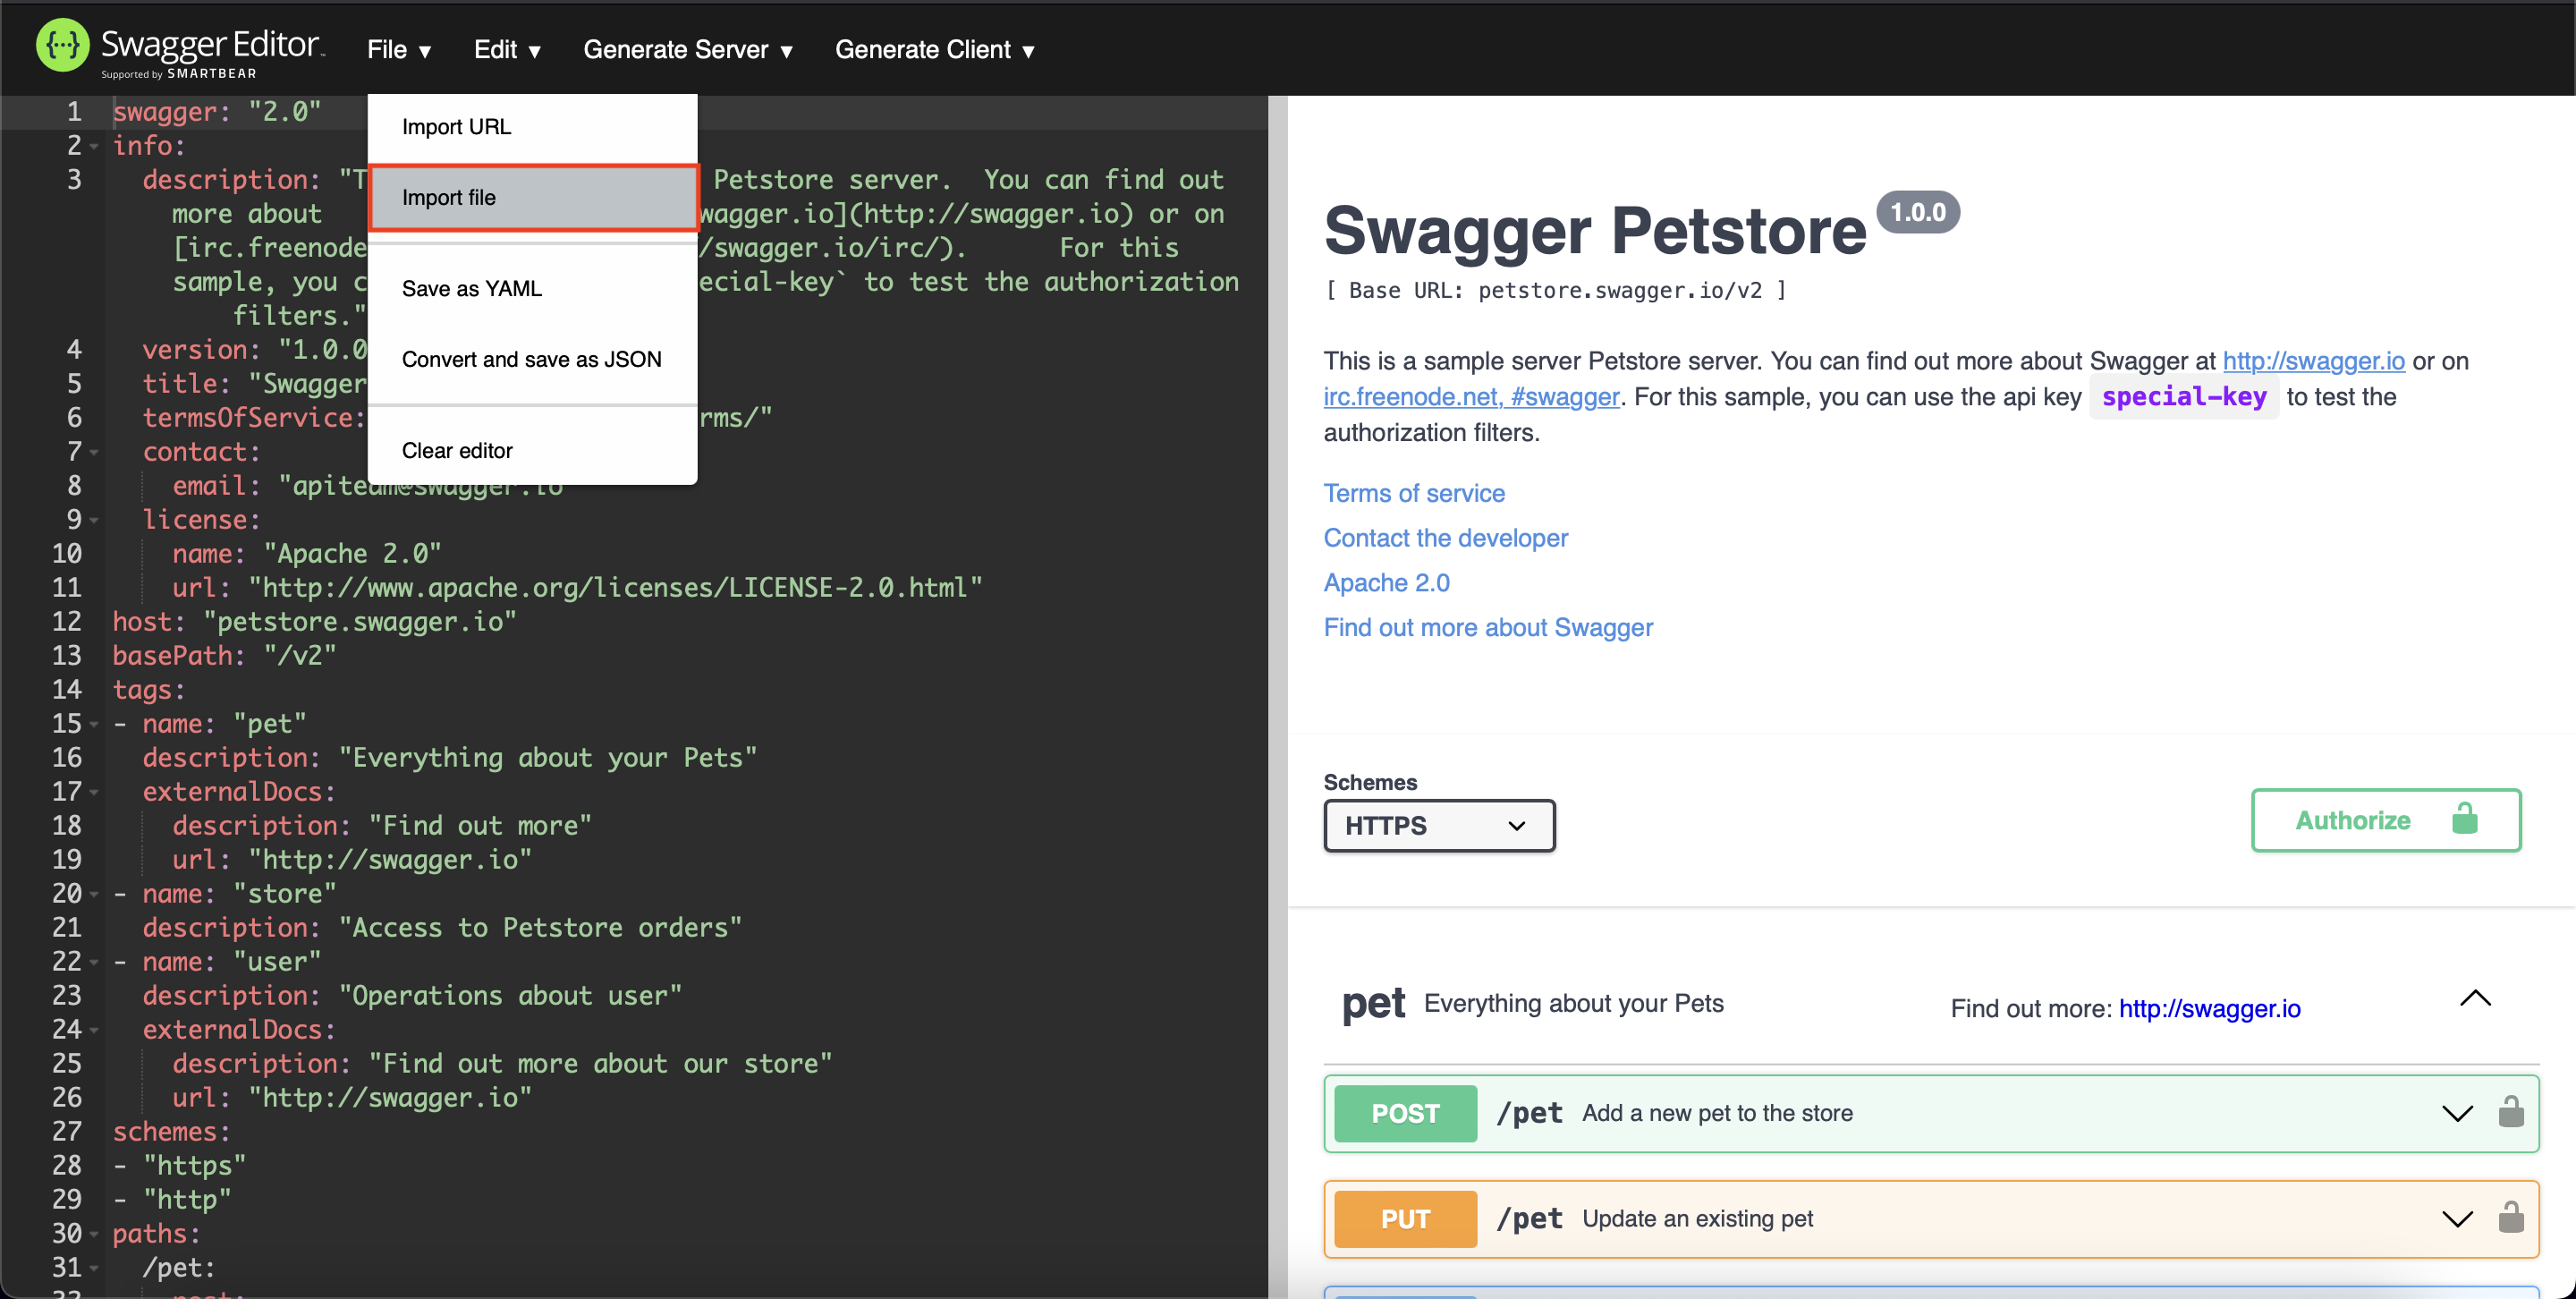
\includegraphics[width=\textwidth]{images/A-navrh-api/A-1-swagger-import.png}
    \caption{Vložení souboru do editoru Swagger}
\end{figure}

\begin{figure}
    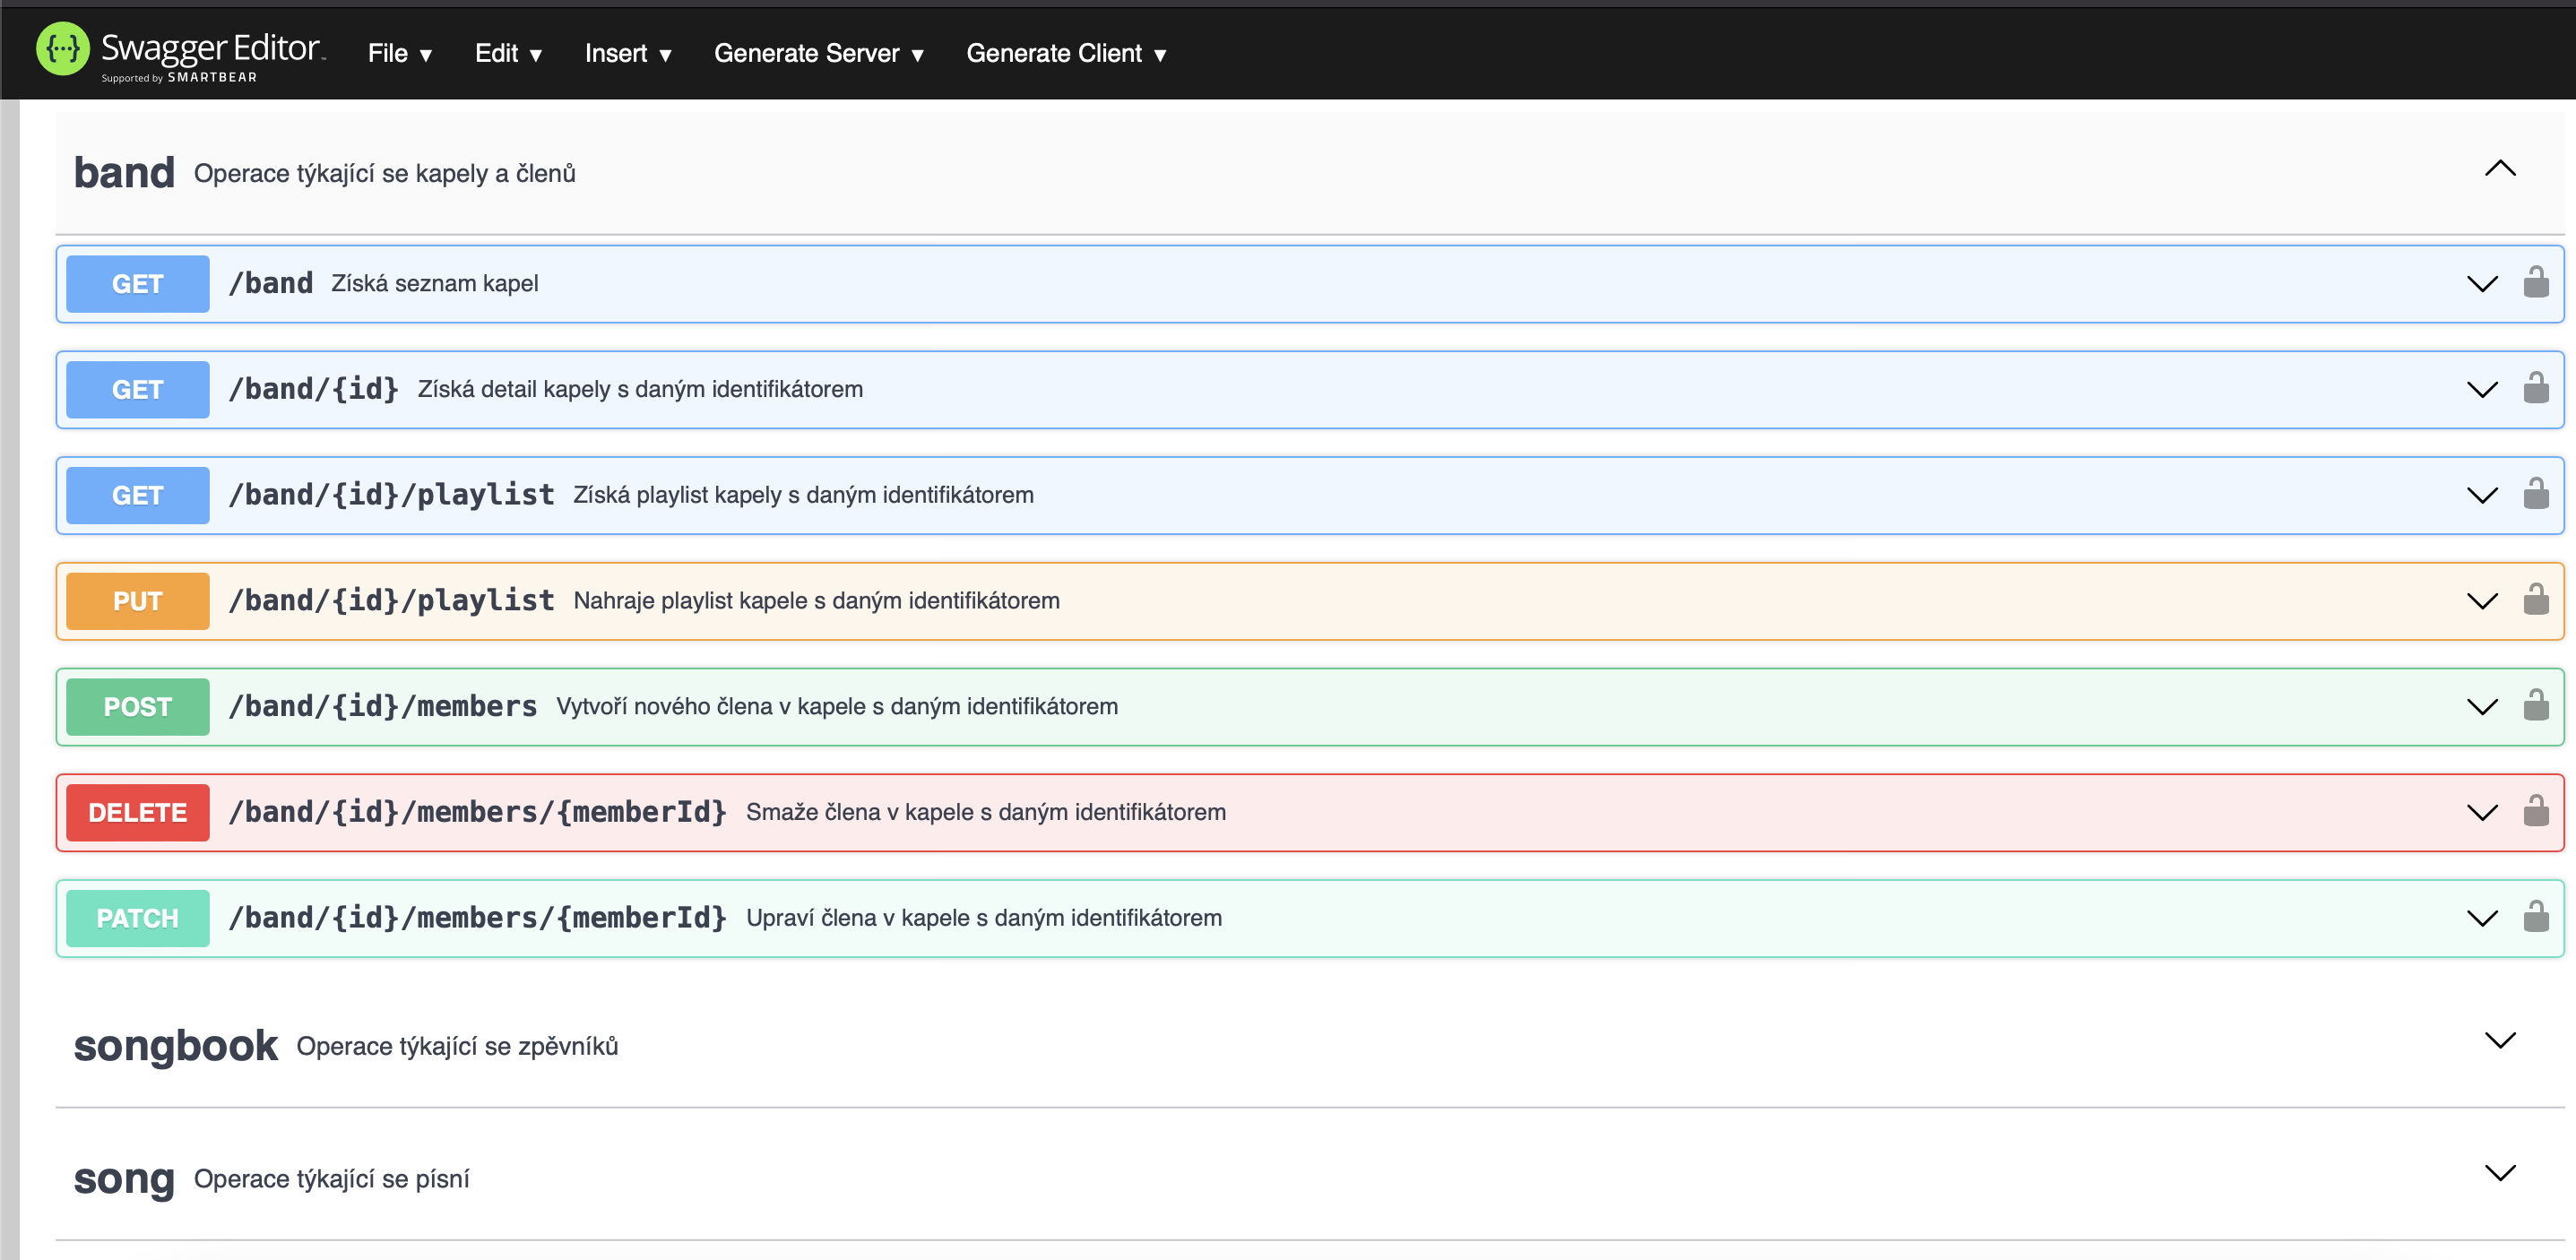
\includegraphics[width=\textwidth]{images/A-navrh-api/A-2-swagger-dokumentace.png}
    \caption{Ukázka vygenerované interaktivní dokumentace v editoru Swagger}
\end{figure}

\begin{figure}
    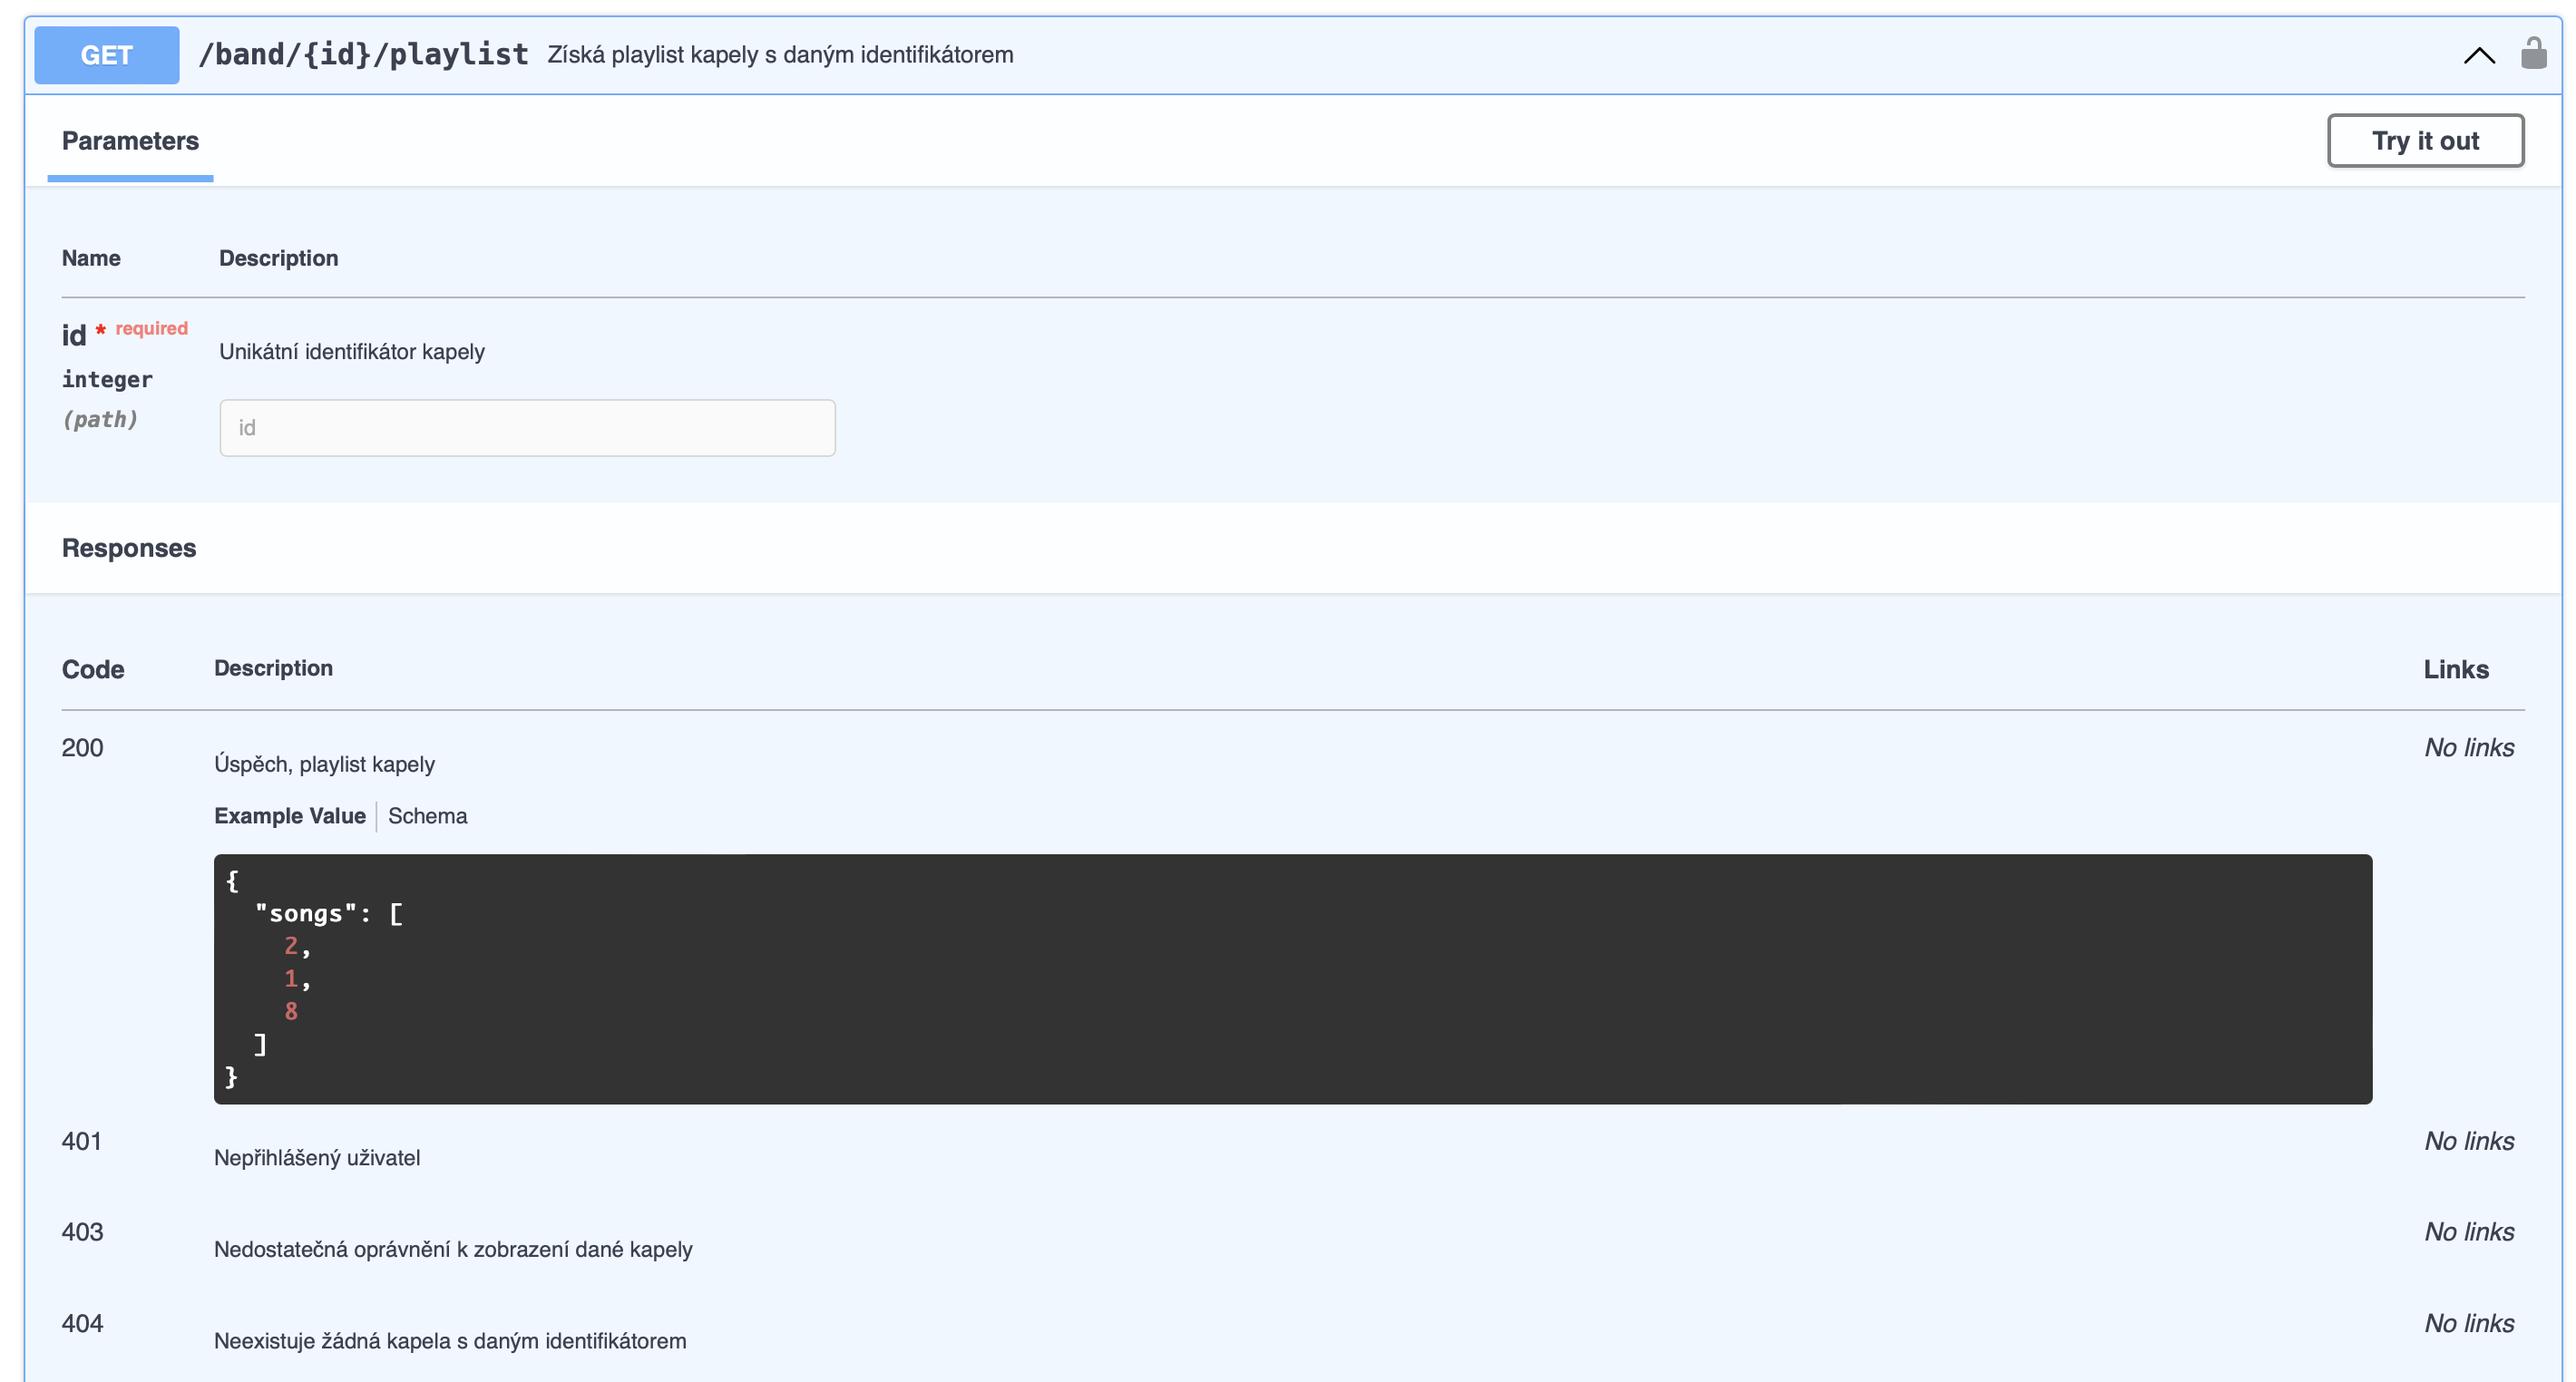
\includegraphics[width=\textwidth]{images/A-navrh-api/A-3-swagger-dokumentace-detail.png}
    \caption{Detail vygenerované dokumentace v editoru Swagger}
\end{figure}

\chapter{Návrh uživatelského rozhraní}

\begin{figure}[H]
    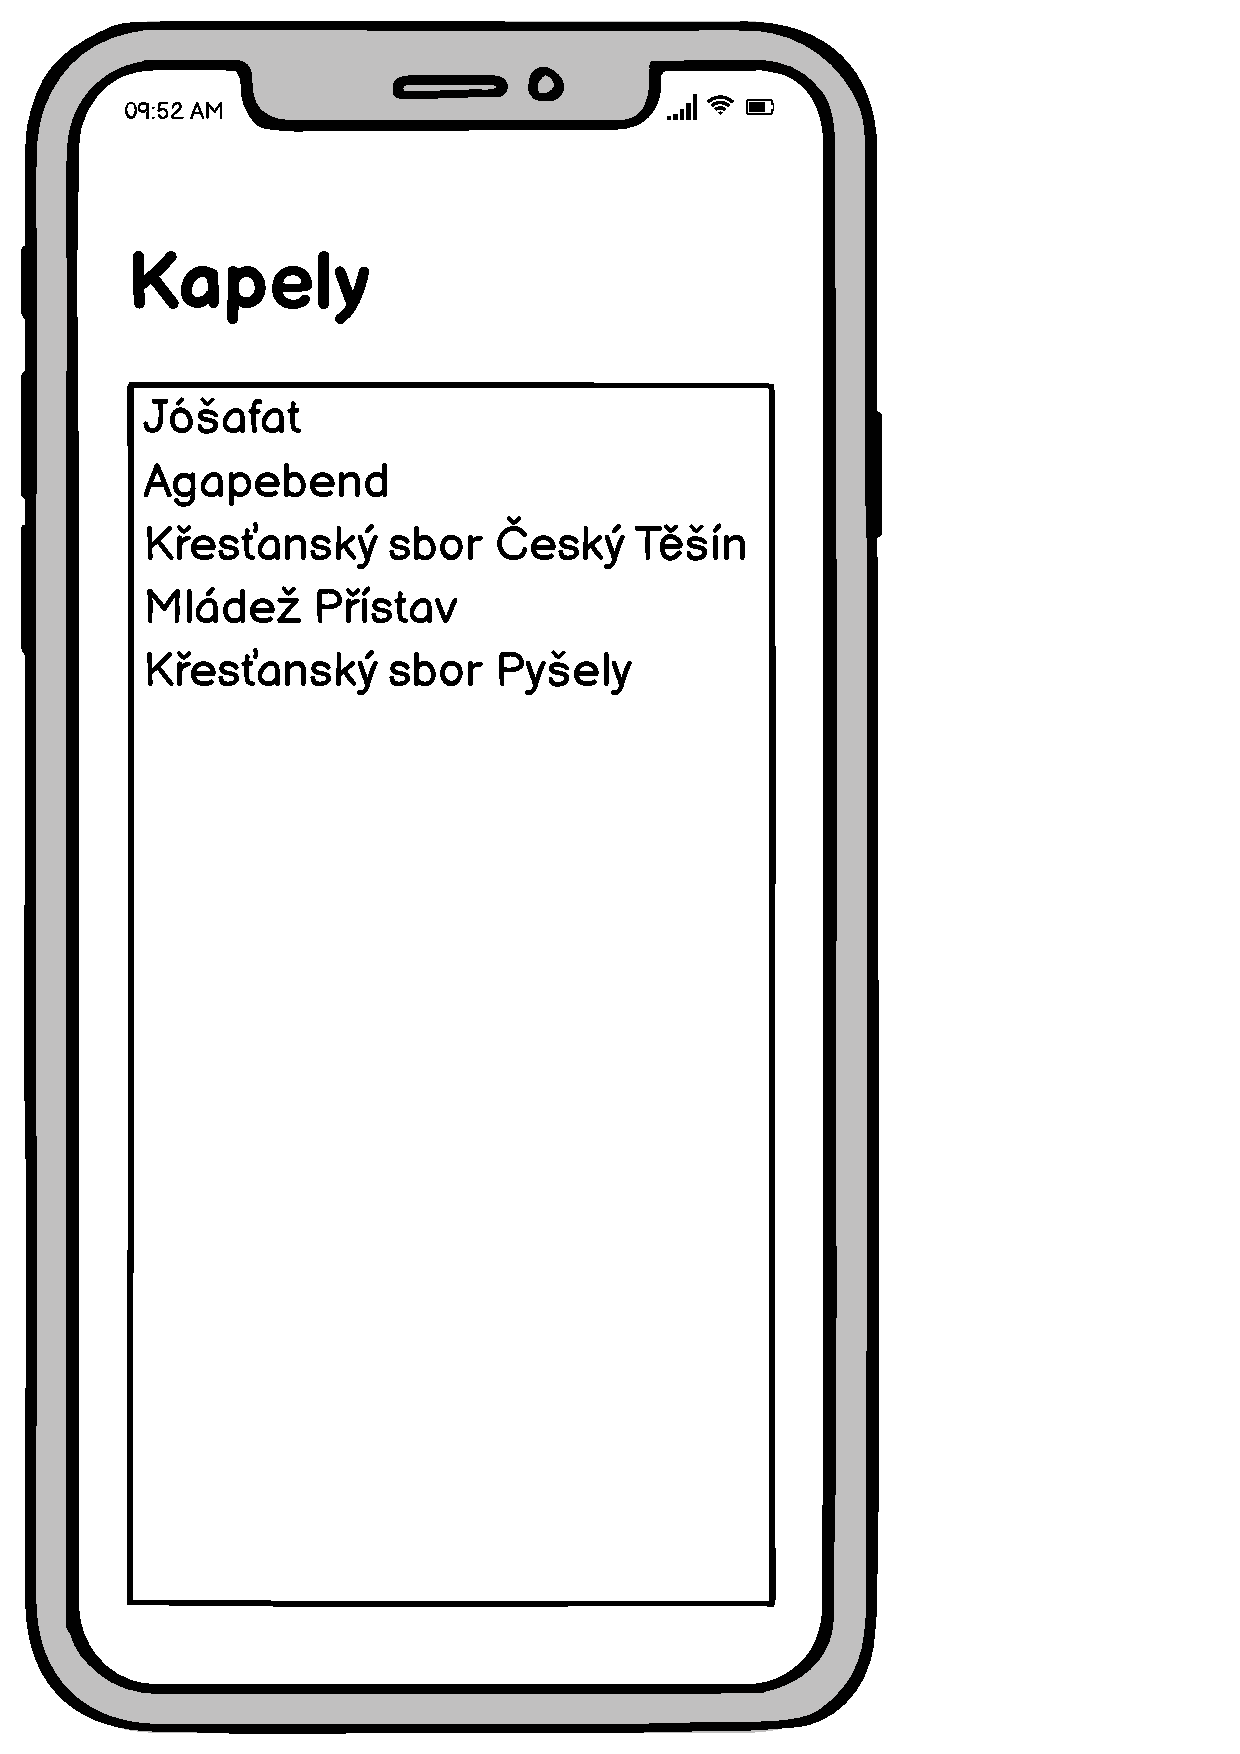
\includegraphics[width=0.45\textwidth]{images/B-navrh-ui/B-1-vyber-kapely.pdf}
    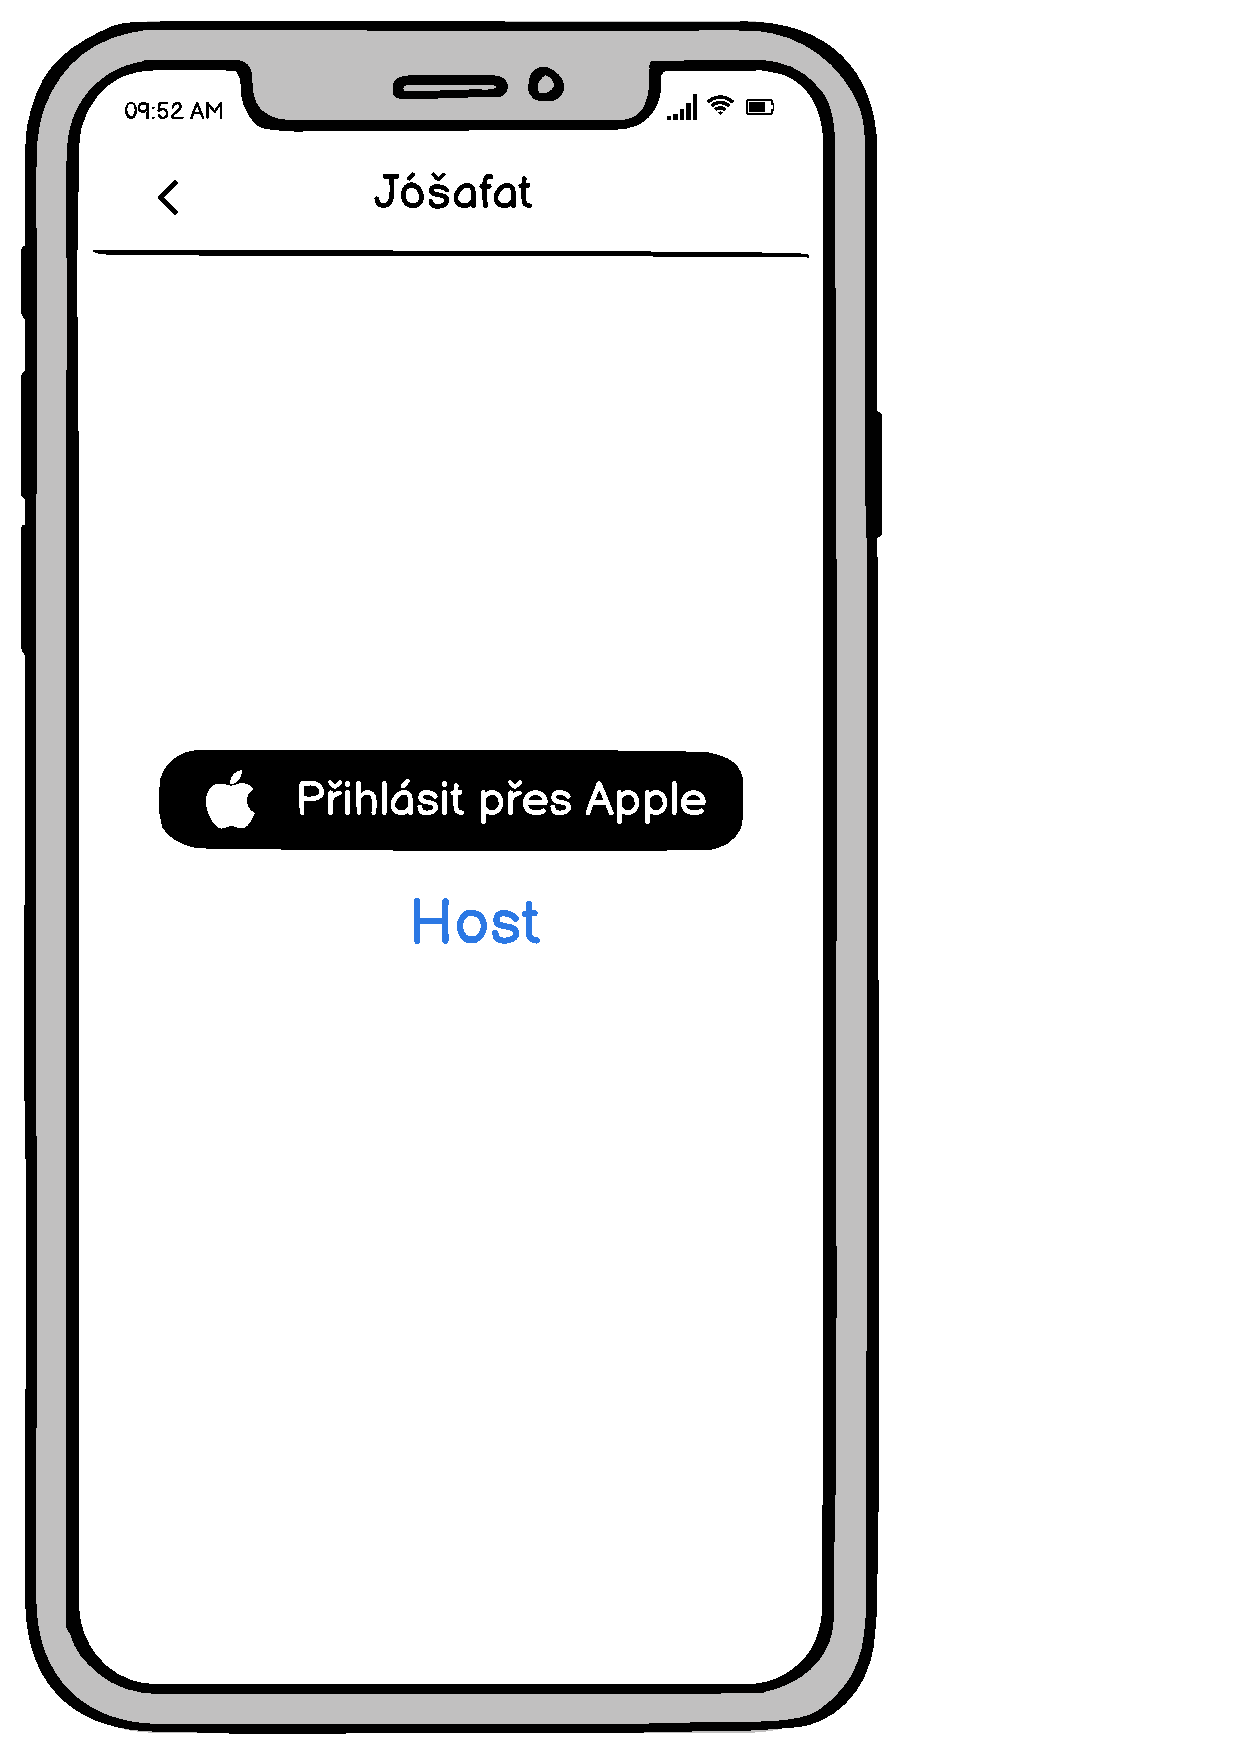
\includegraphics[width=0.45\textwidth]{images/B-navrh-ui/B-1-prihlaseni.pdf}
    \caption{Výběr kapely a Přihlášení}
\end{figure}

% Stránka 2

\begin{figure}
    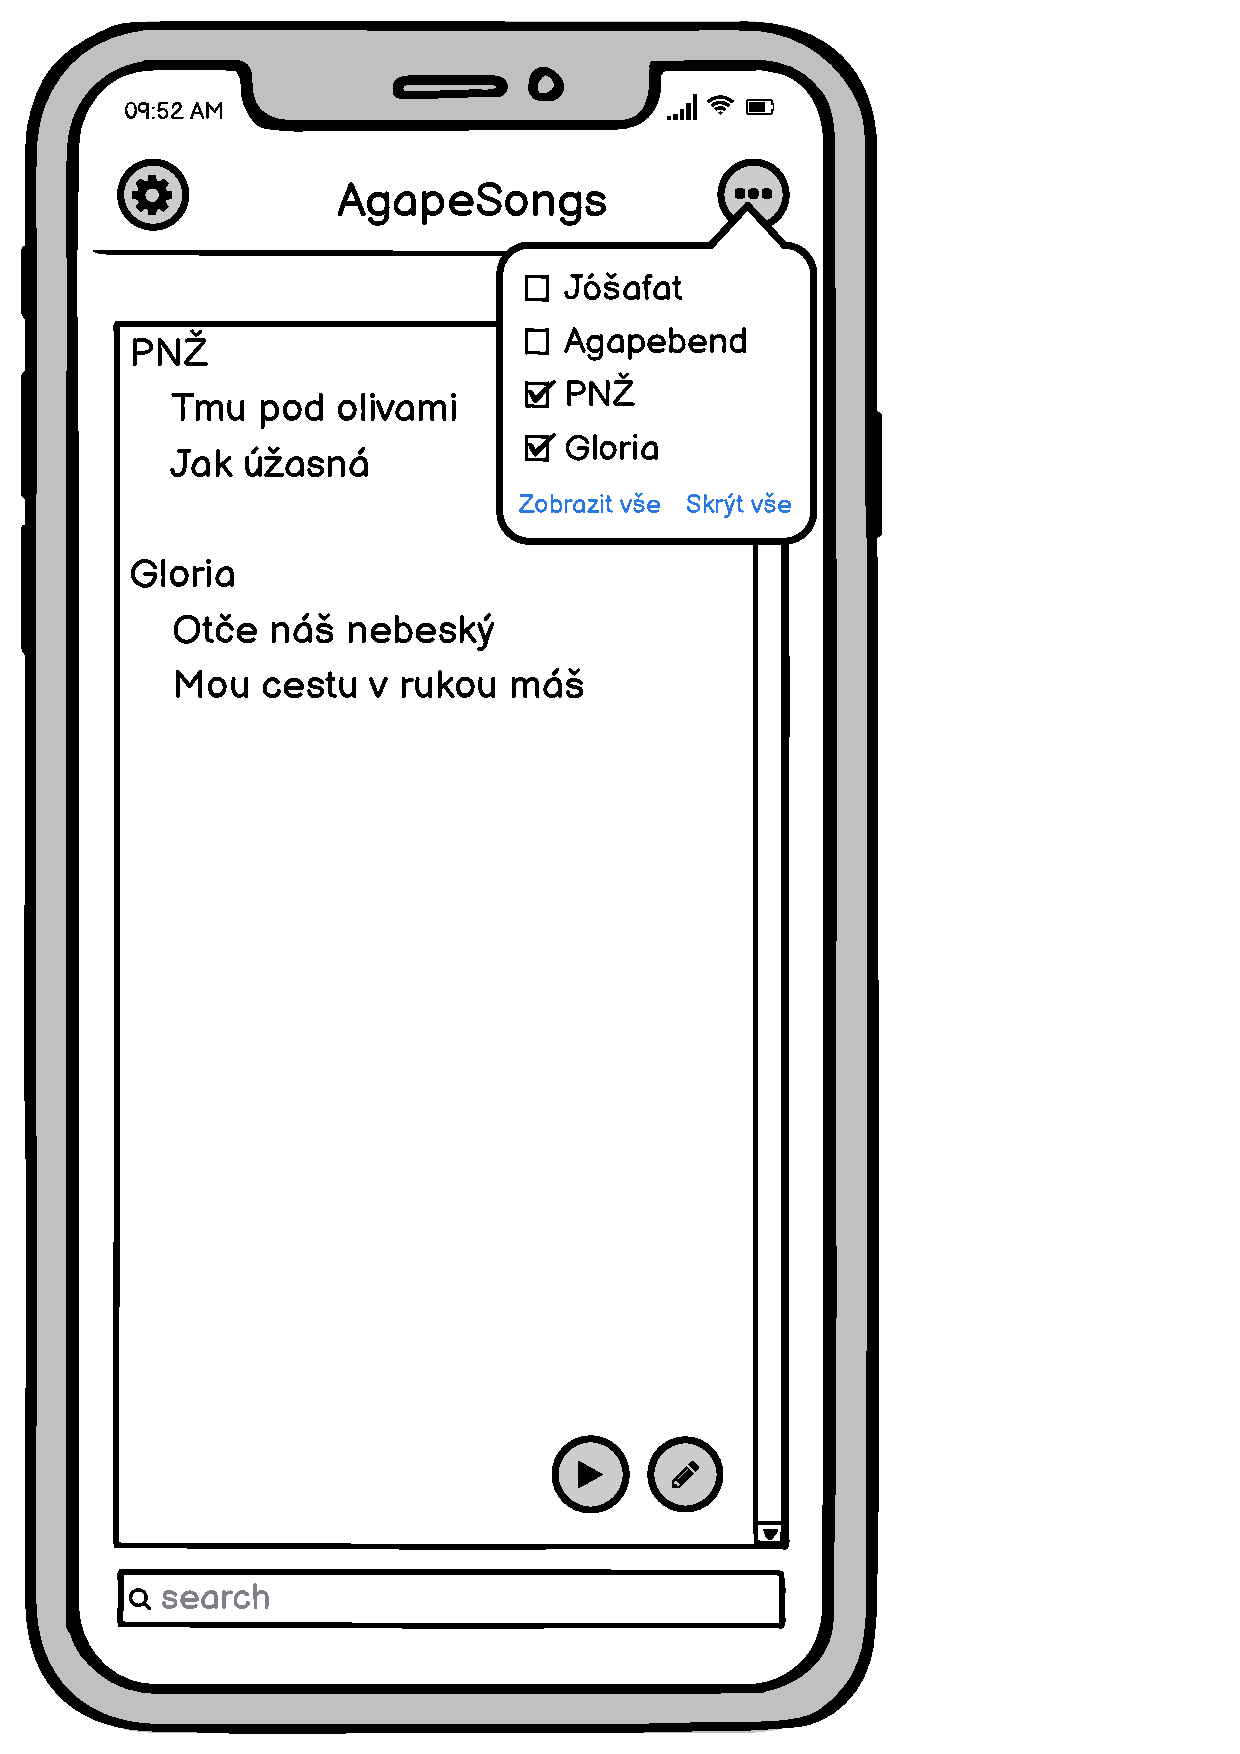
\includegraphics[width=0.49\textwidth]{images/B-navrh-ui/B-2-seznam-pisni.pdf}
    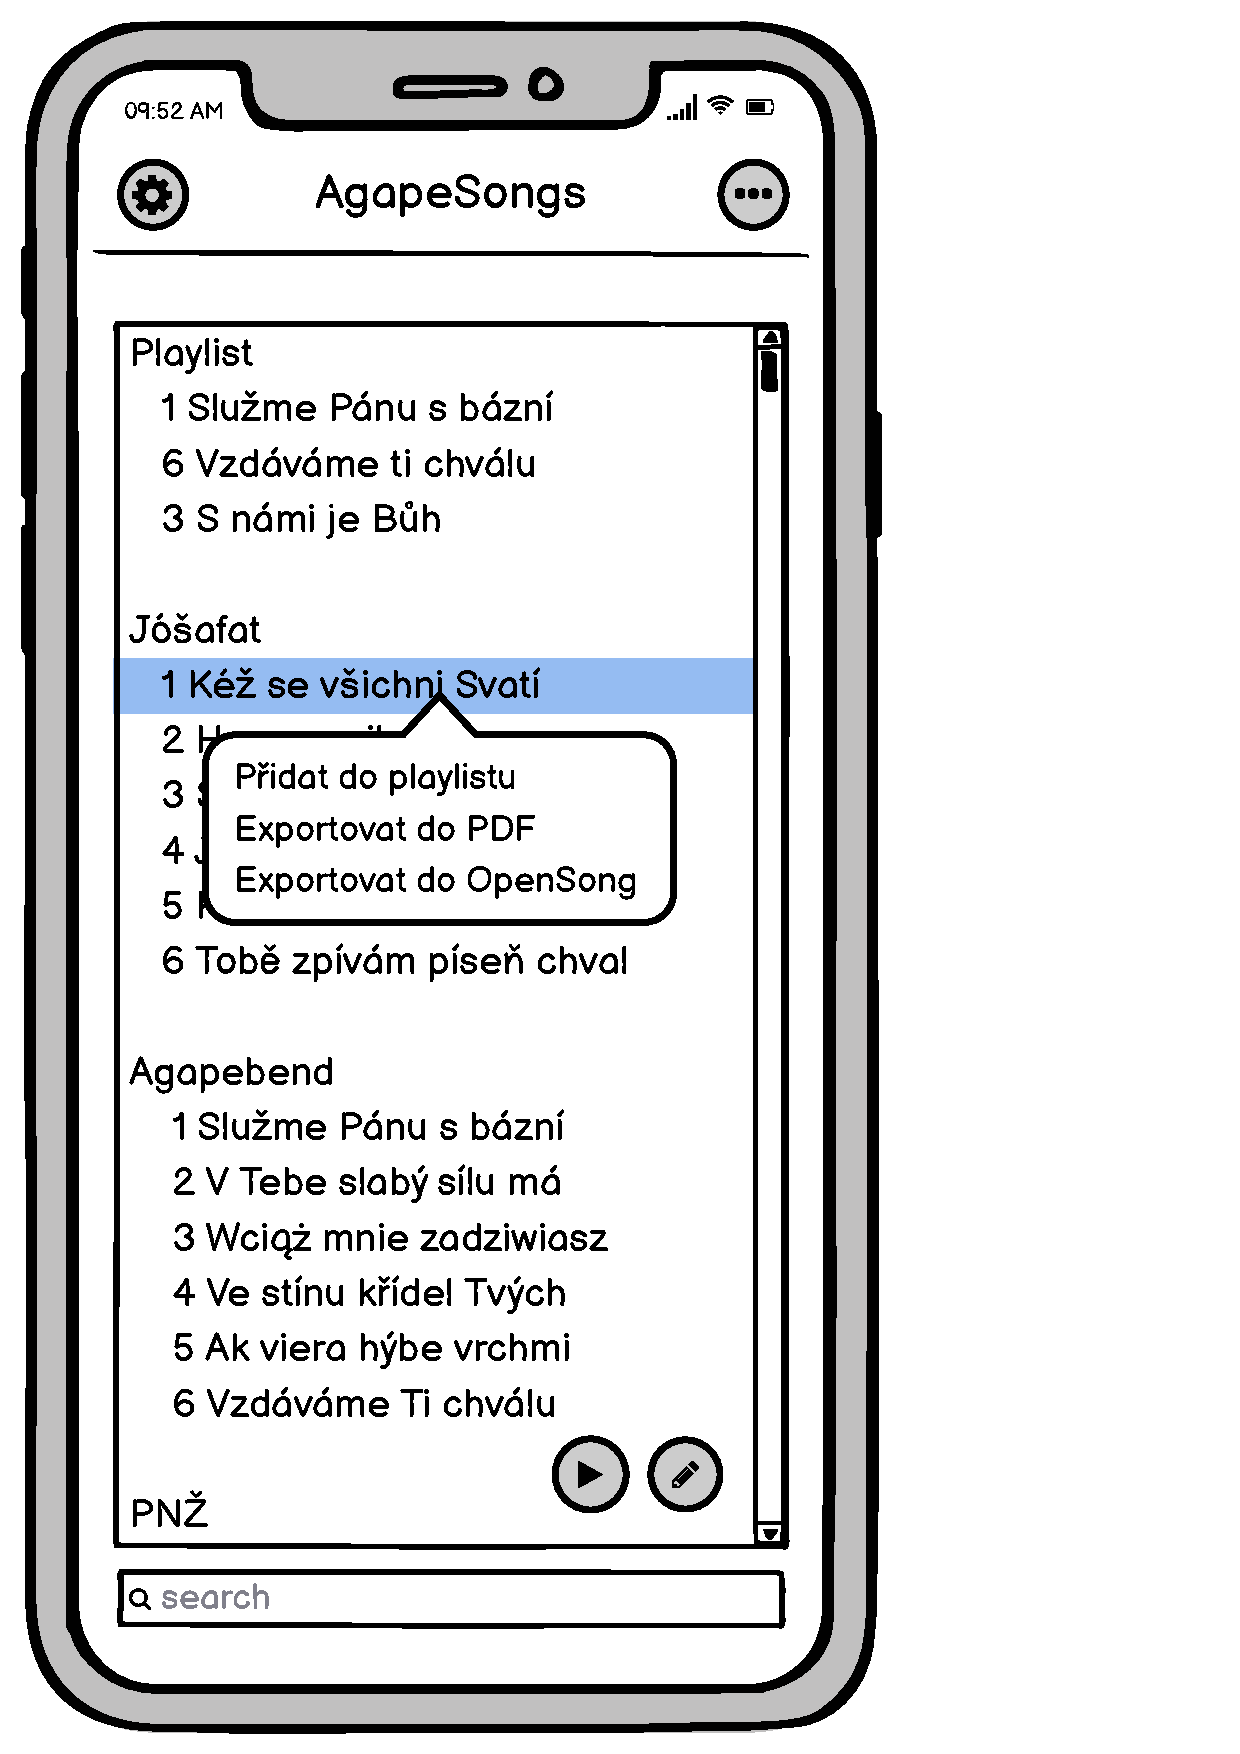
\includegraphics[width=0.49\textwidth]{images/B-navrh-ui/B-2-seznam-pisni-kontextove-menu.pdf}
    \caption{Seznam písní a kontextové menu pro přidání písně do playlistu a export písně}
\end{figure}

% Stránka 3

\begin{figure}
    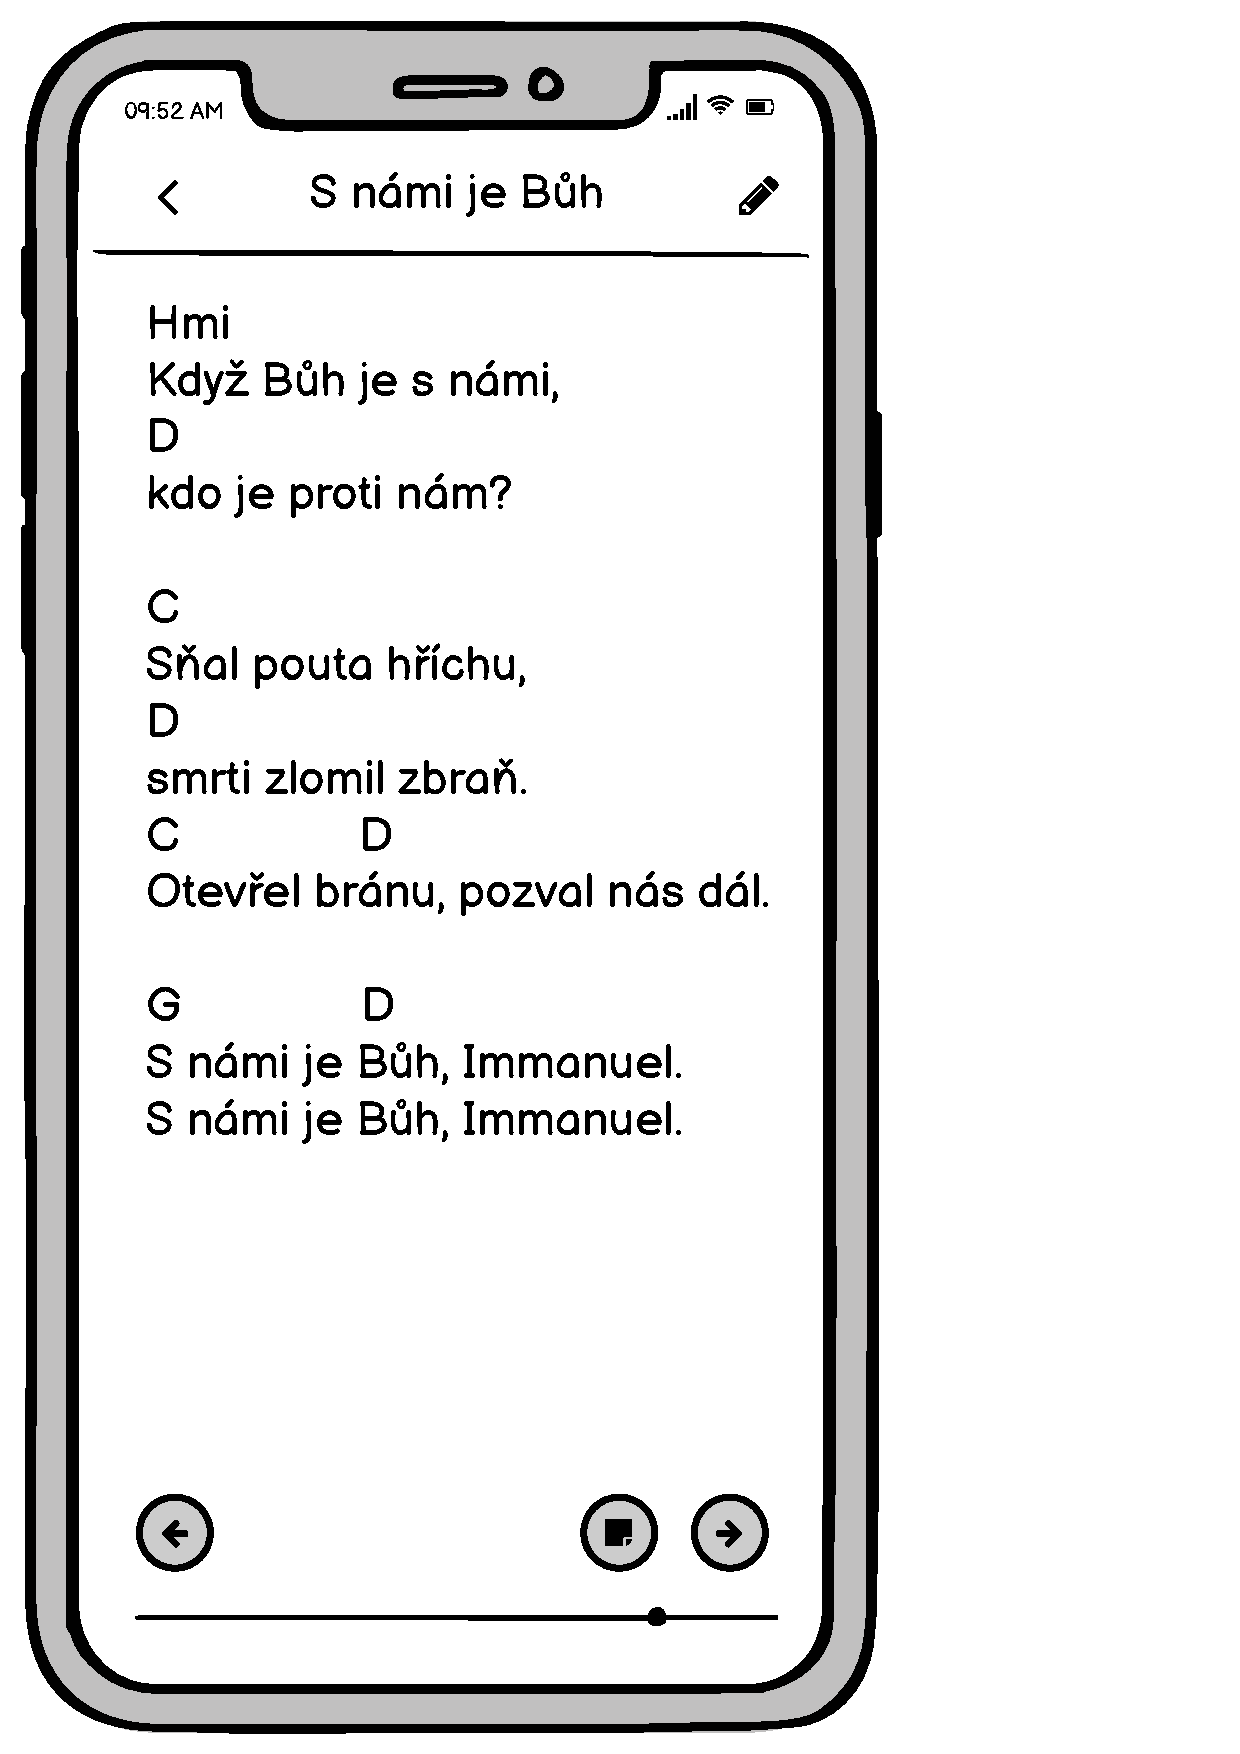
\includegraphics[width=0.49\textwidth]{images/B-navrh-ui/B-3-detail-pisne.pdf}
    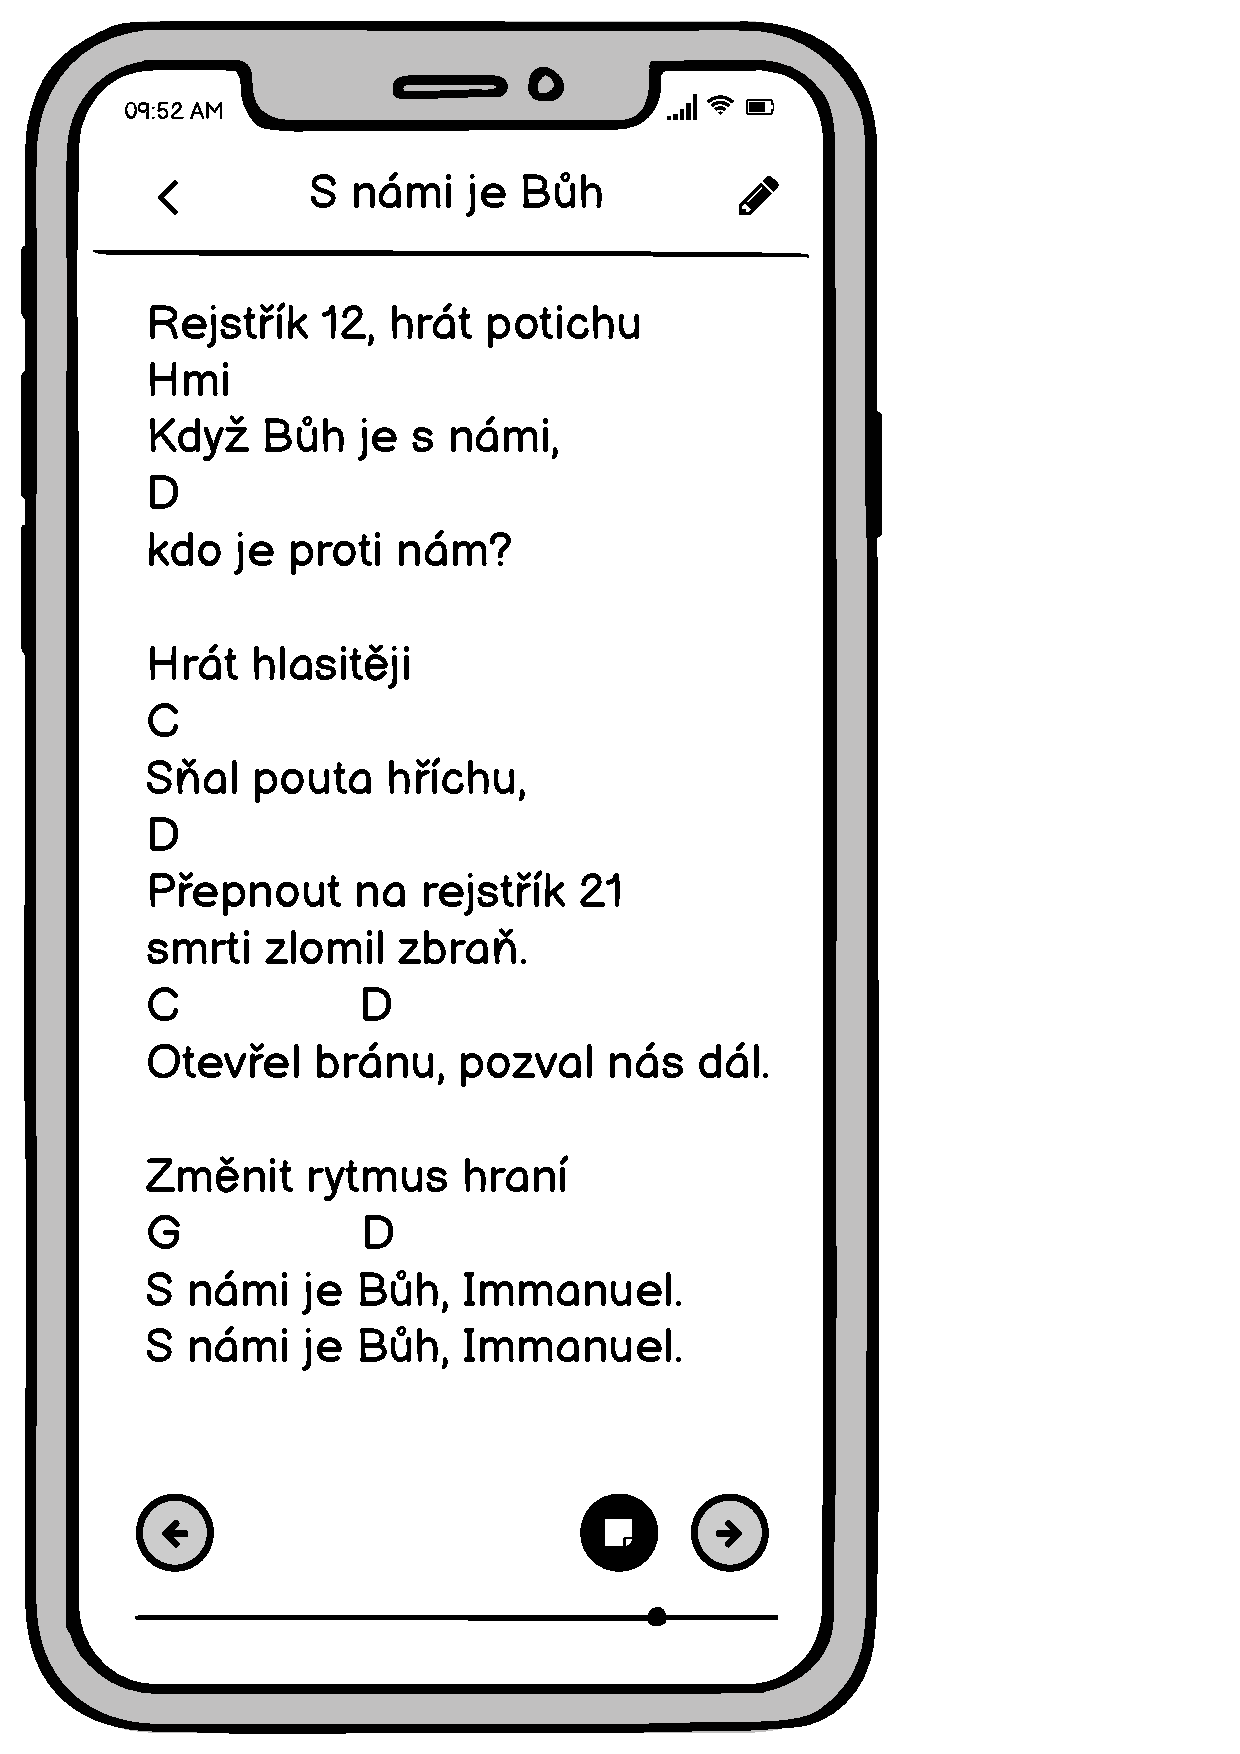
\includegraphics[width=0.49\textwidth]{images/B-navrh-ui/B-3-detail-pisne-poznamky.pdf}
    \caption{Detail písně bez a se zapnutými poznámkami}
\end{figure}

% Stránka 4

\begin{figure}
    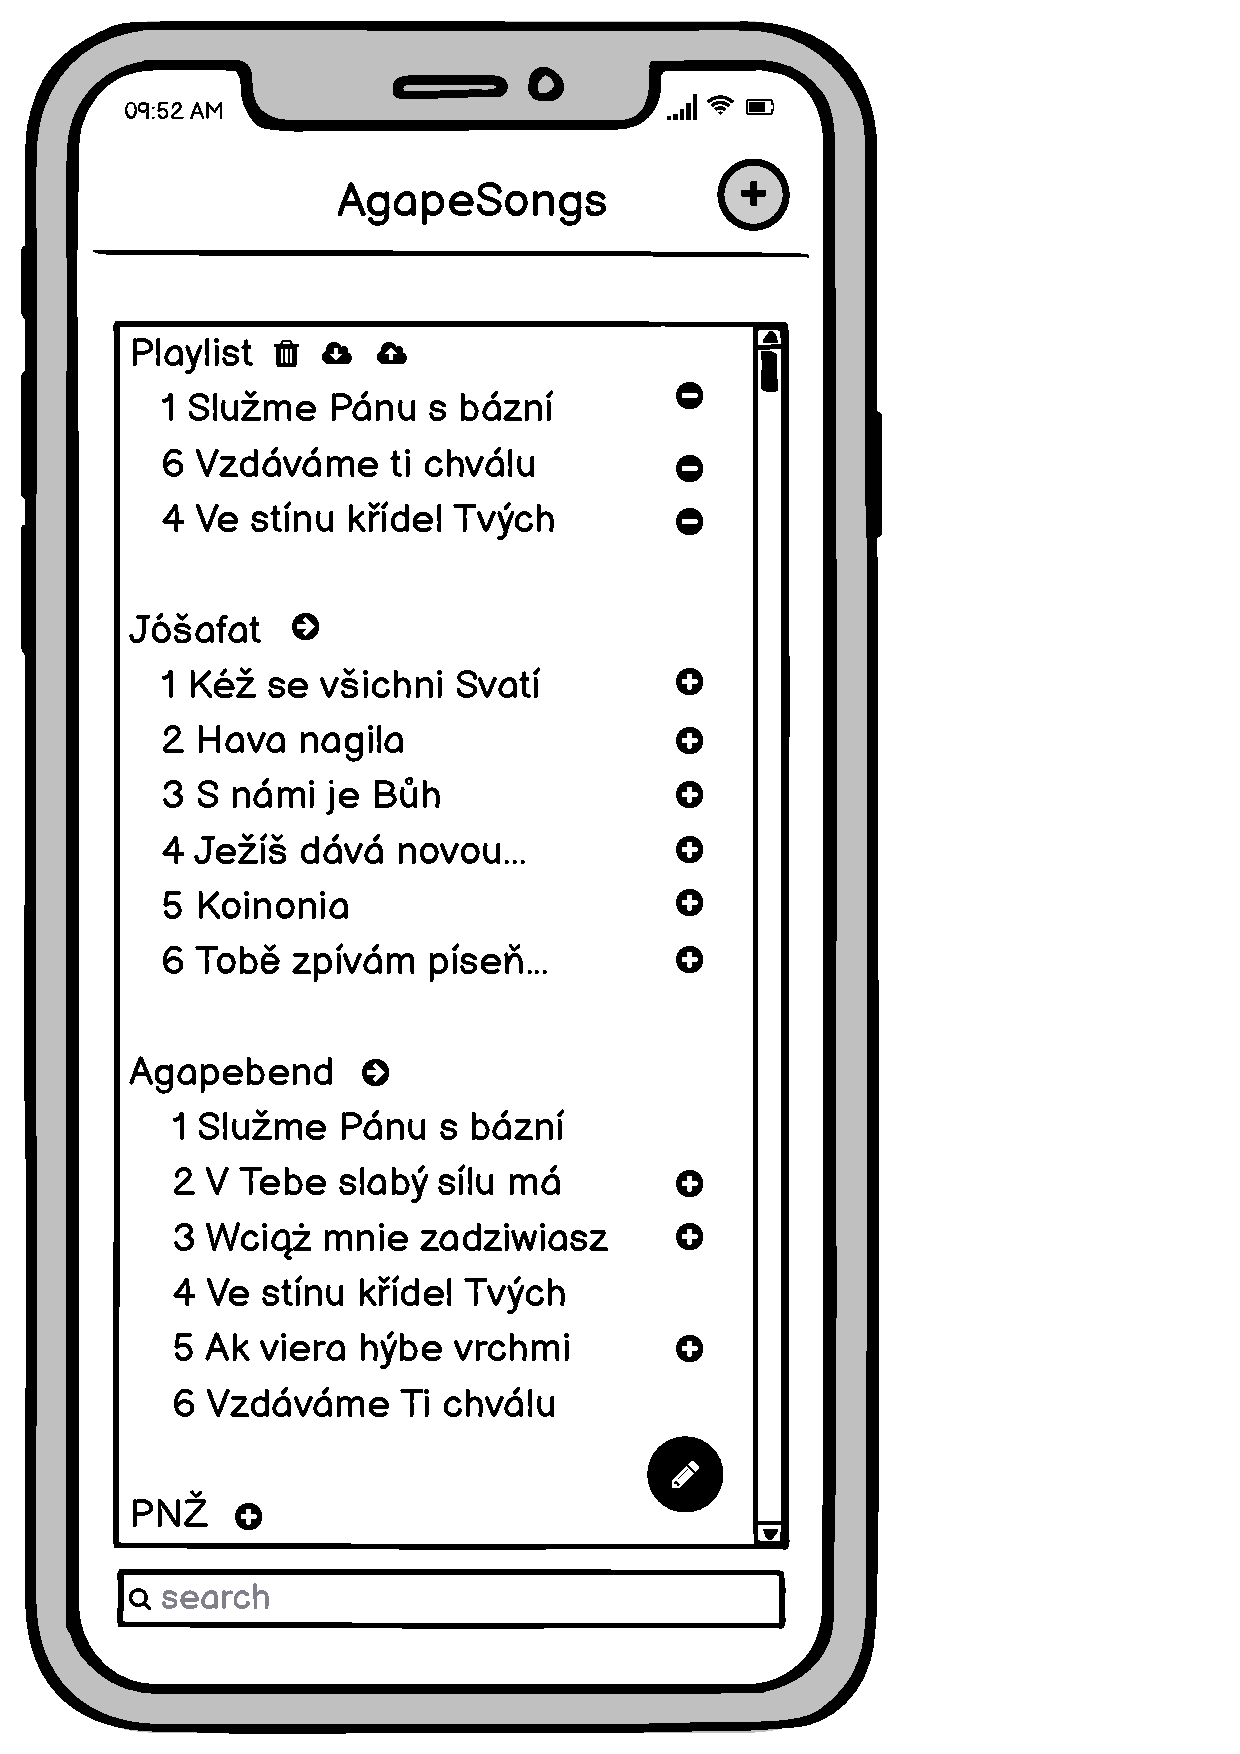
\includegraphics[width=0.49\textwidth]{images/B-navrh-ui/B-4-sprava-playlistu-zpevniku.pdf}
    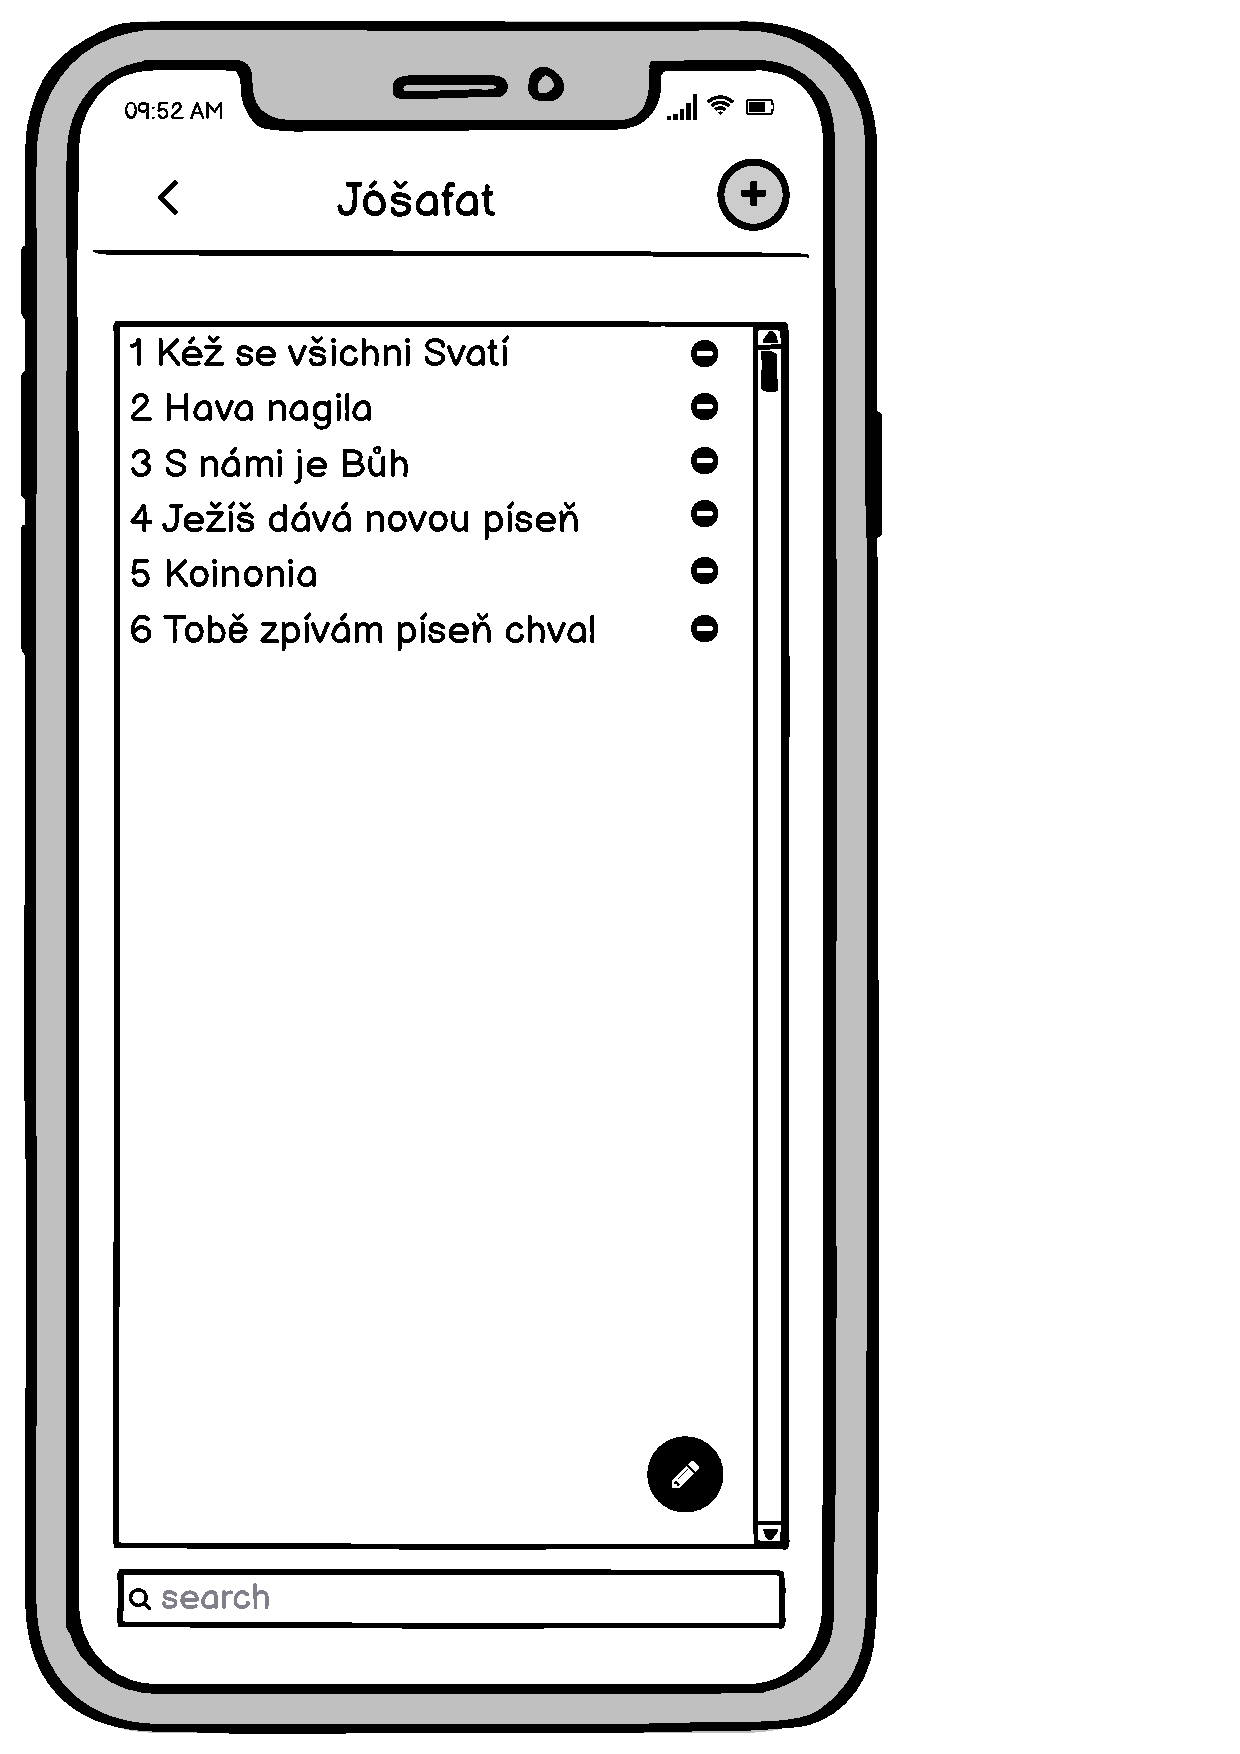
\includegraphics[width=0.49\textwidth]{images/B-navrh-ui/B-4-sprava-pisni.pdf}
    \caption{Správa playlistů, zpěvníků a Správa písní ve zpěvníku}
\end{figure}

% Stránka 5

\begin{figure}
    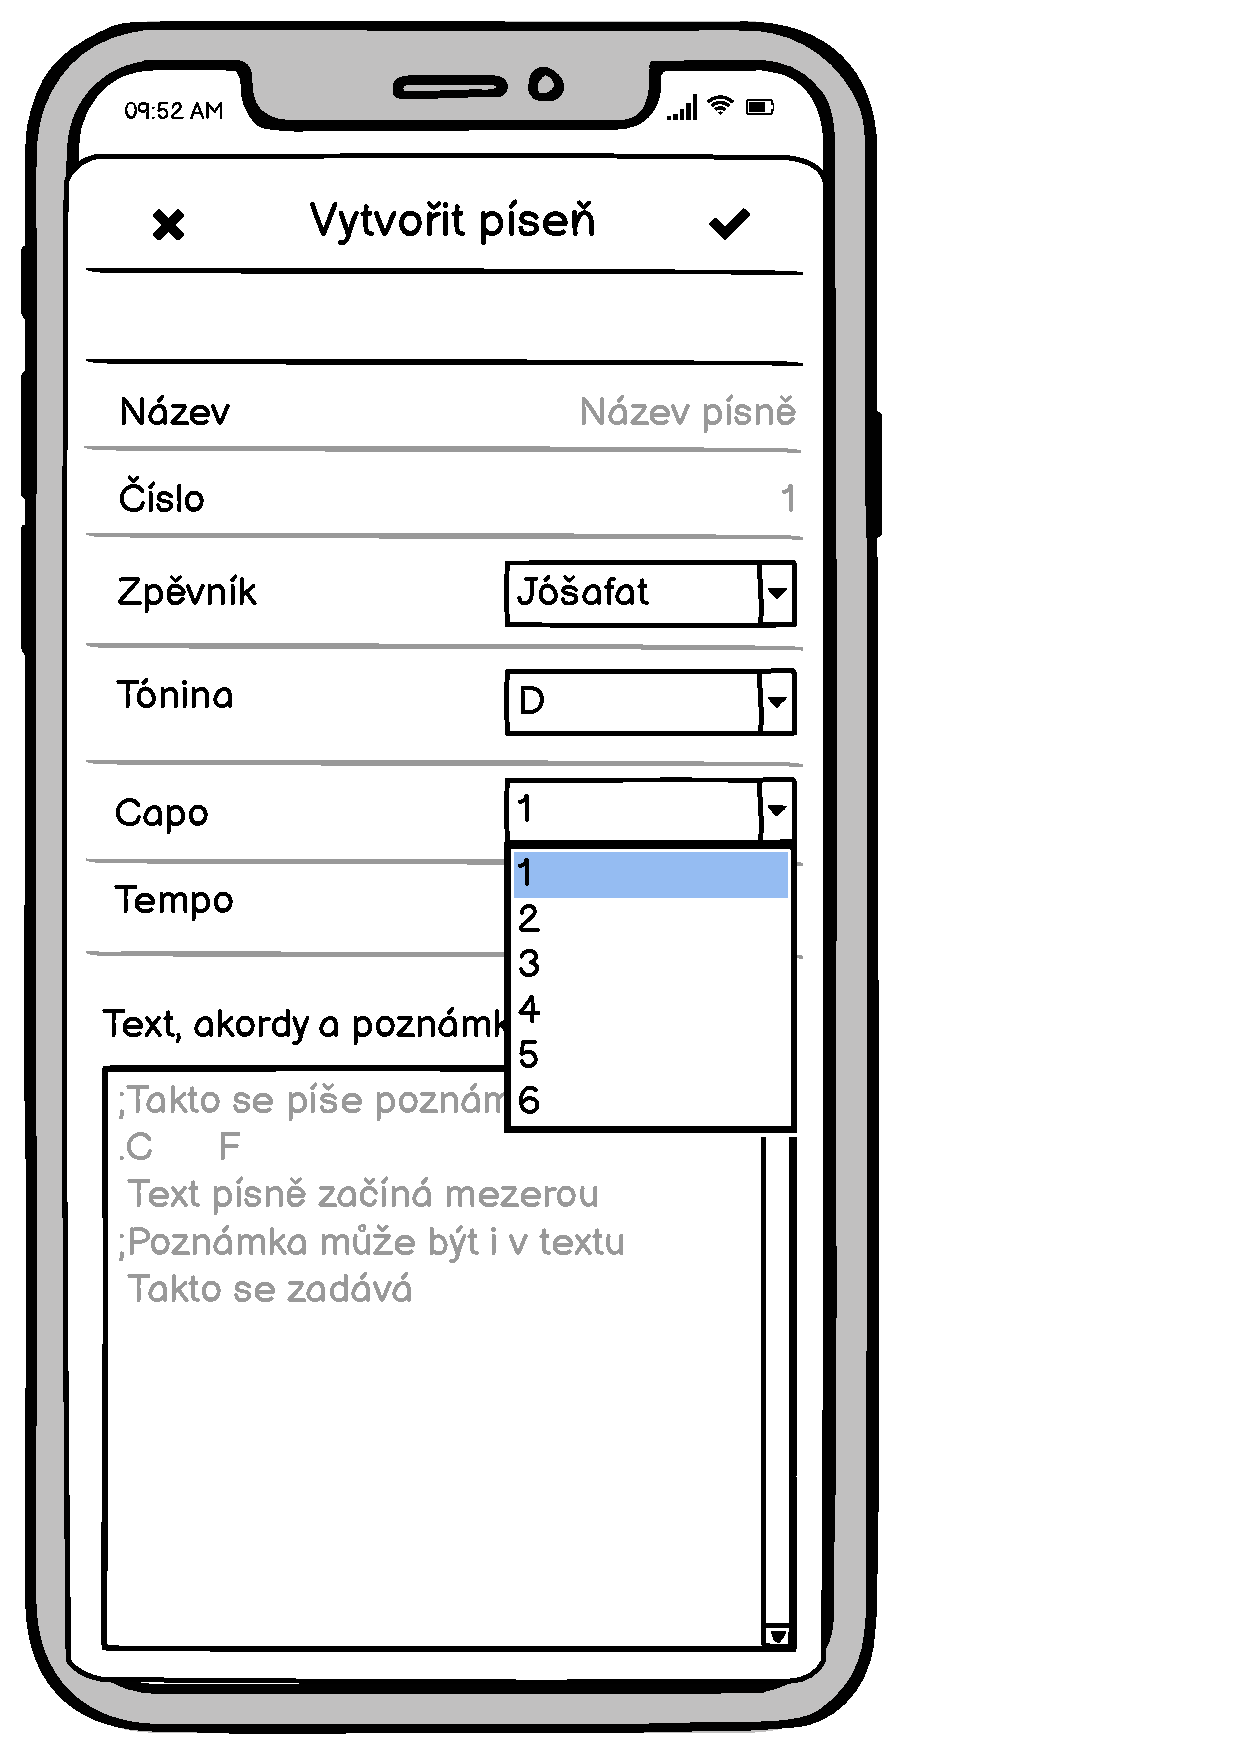
\includegraphics[width=0.49\textwidth]{images/B-navrh-ui/B-5-nova-pisen.pdf}
    \includegraphics[width=0.49\textwidth]{images/B-navrh-ui/B-5-smazat-pisen.pdf}
    \caption{Vytvoření/úprava písně a Smazání písně}
\end{figure}

% Stránka 6

\begin{figure}
    \includegraphics[width=0.49\textwidth]{images/B-navrh-ui/B-6-sprava-kapely.pdf}
    \includegraphics[width=0.49\textwidth]{images/B-navrh-ui/B-6-zmena-role.pdf}
    \caption{Správa kapely a dialog pro změnu role člena kapely}
\end{figure}

\chapter{Uživatelské rozhraní}

\begin{figure}[H]
    \includegraphics[width=0.9\textwidth]{images/C-ui/C-1-prihlaseni-seznam-zpevniku.png}
    \caption{Přihlášení a Seznam písní -- filtr zpěvníků}
\end{figure}

% Stránka 2

\begin{figure}
    \includegraphics[width=\textwidth]{images/C-ui/C-2-detail-pisne.png}
    \caption{Detail písně a Nastavení písně}
\end{figure}

% Stránka 3

\begin{figure}
    \includegraphics[width=\textwidth]{images/C-ui/C-3-sprava-zpevniku-pisni.png}
    \caption{Správa playlistů, zpěvníků a Správa písní ve zpěvníku}
\end{figure}

% Stránka 4

\begin{figure}
    \includegraphics[width=\textwidth]{images/C-ui/C-4-nova-pisen-smazani-pisne.png}
    \caption{Vytvoření/úprava písně a Smazání písně}
\end{figure}

% Stránka 5

\begin{figure}
    \includegraphics[width=\textwidth]{images/C-ui/C-5-nastaveni-aplikace-sprava-kapely.png}
    \caption{Nastavení aplikace a Správa kapely}
\end{figure}

\backmatter

% include bibliography
\printbibliography

% include medium
\chapter{Obsah přiloženého média}
	\dirtree{%
		.1 readme.txt\DTcomment{stručný popis obsahu média}.
		.1 design.
		.2 diagram.eapx\DTcomment{Enterprise Architect projekt s diagramy}.
		.2 rest.yaml\DTcomment{návrh REST API ve formátu YAML}.
		.2 ui.bpmr\DTcomment{Balsamiq projekt s návrhem uživatelského rozhraní}.
		.1 src.
		.2 backend\DTcomment{zdrojové kódy serveru}.
		.2 frontend\DTcomment{zdrojové kódy mobilní aplikace}.
		.2 thesis\DTcomment{zdrojová forma práce ve formátu \LaTeX{}}.
		.1 text\DTcomment{text práce}.
		.2 thesis.pdf\DTcomment{text práce ve formátu PDF}.
	}


\end{document}
